% Copyright (c) 2008-2009 solvethis
% Copyright (c) 2010-2016,2018-2019,2022 Casper Ti. Vector
% Copyright (c) 2021 Kurapica
% Copyright (c) 2022 iofu728
% Overleaf version.

%*********************************************************************
% iofu728-pkuthss: 北京大学研究生学位论文模板
% 2022/07/16 v1.1.0
%
% 重要提示:
%   1. 当前overleaf版符合2022研究生学位论文要求,可通过图书馆审核
%   2. 当前版本基于pkuthss v1.9.2
%   3. 请使用UTF-8编码,XeLaTeX方式编译
%   4. 请仔细阅读用户文档
%   5. 修改、使用、发布本文档类请务必遵循LaTeX Project Public License和知识共享4.0
%   6. 如有疑问github/iofu728/pkuthss上提问或联系作者@iofu728
%*********************************************************************

\documentclass[fontset=fandol,ugly,language=chinese]{pkuthss}
  % 学位论文模式  ugly    (默认打开,请保留)
  % 盲审模式     blind   (默认关闭)
  % 语言        language (默认chinese | english)
  % 字体库       fontset
  %   auto | windows | windows@overleaf | mac | fandol | ubuntu | none
  % windows*, mac为商业字体,如需使用请遵循相应版权协议(默认下overleaf中不可用)
  % fandol与windows效果相近,但字符库偏少,推荐使用(默认);
  % ubuntu字体效果偏差较大; 设为none时需自行配置字体集;

\usepackage[backend=biber,style=gb7714-2015,gbnamefmt=lowercase,doi=false,gbtype=false,url=false,gbnamefmt=familyahead]{biblatex}  
% 参考文献遵循GB/T 7714-2015标准,使用biblatex-gb7714-2015 宏包。
  % 此处使用顺序编码制,如使用著者-出版年制则更改为b7714-2015ay。

% 示例文档用包和设定,该段均可移除.
\usepackage{enumitem,fancyvrb}
\usepackage{booktabs,multirow,longtable,makecell} % 表格相关
\RecustomVerbatimEnvironment{Verbatim}{Verbatim}{frame = single, tabsize = 4, fontsize=\footnotesize}
\renewcommand{\v}[1]{\boldsymbol{#1}}
\newcommand\pkg[1]{\textsf{#1}}

% make sure figures are inside there own sections
\usepackage[section]{placeins}

\providecommand{\CHECK}[1]{{\protect\color{orange}\it{#1}}}

% 插入代码
\usepackage{listings}


% 参考文献边距字体
\setlength{\bibitemsep}{3bp}
\renewcommand*{\bibfont}{\zihao{5}\linespread{1.27}\selectfont}

\pkuthssinfo{
    cthesisname = {博士学位论文},
    thesiscover = {博士研究生学位论文},
    ethesisname = {Doctoral Dissertation},
    ctitle = {新一代深海中微子望远镜的设计优化},
    etitle = {Optimizing a Next Generation Deep Sea Neutrino Telescope},
    cauthor = {胡帆}, eauthor = {Fan Hu},
    studentid = {1801110211},
    % 具体时间以教务为准,初稿3月,送审4月,答辩5月,最终6月。
    date = {\zhdigits{2023}\ \ 年\ \ \zhnumber{4}\ \ 月}, % June, 2022
    school = {物理学院},
    cmajor = {天体物理}, emajor = {Astrophysics},
    direction = {粒子天体物理},
    mentorlines = {2}, % 导师个数
    % 副教授 A.P. 讲师 Lec.
    cmentor = {黎卓 \ \ 副教授\\ 徐东莲\ \ 李政道学者}, ementor = {Prof.\ Zhuo, Li and Prof.\ Xu, Donglian},
    ckeywords = {中微子天文学;中微子望远镜;粒子模拟;探测器模拟;深海实验},
    ekeywords = {neutrino astronomy, Neutrino telescope, particle simulation, detector simulation, deep-sea experiment},
    % 盲审模式参数, 需在documentclass增加blind
    blindid = {XXXXXXXXX}, discipline = {XXXX}
}
\addbibresource{a_ref.bib}


\begin{document}
    \frontmatter
    \pagestyle{empty}
    \maketitle
    \cleardoublepage
    % 需替换门户版权声明pdf
    % Copyright (c) 2008-2009 solvethis
% Copyright (c) 2010-2017,2021 Casper Ti. Vector
% Copyright (c) 2021 iofu728
% All rights reserved.
%
% Redistribution and use in source and binary forms, with or without
% modification, are permitted provided that the following conditions are
% met:
%
% * Redistributions of source code must retain the above copyright notice,
%   this list of conditions and the following disclaimer.
% * Redistributions in binary form must reproduce the above copyright
%   notice, this list of conditions and the following disclaimer in the
%   documentation and/or other materials provided with the distribution.
% * Neither the name of Peking University nor the names of its contributors
%   may be used to endorse or promote products derived from this software
%   without specific prior written permission.
%
% THIS SOFTWARE IS PROVIDED BY THE COPYRIGHT HOLDERS AND CONTRIBUTORS "AS
% IS" AND ANY EXPRESS OR IMPLIED WARRANTIES, INCLUDING, BUT NOT LIMITED TO,
% THE IMPLIED WARRANTIES OF MERCHANTABILITY AND FITNESS FOR A PARTICULAR
% PURPOSE ARE DISCLAIMED. IN NO EVENT SHALL THE COPYRIGHT HOLDER OR
% CONTRIBUTORS BE LIABLE FOR ANY DIRECT, INDIRECT, INCIDENTAL, SPECIAL,
% EXEMPLARY, OR CONSEQUENTIAL DAMAGES (INCLUDING, BUT NOT LIMITED TO,
% PROCUREMENT OF SUBSTITUTE GOODS OR SERVICES; LOSS OF USE, DATA, OR
% PROFITS; OR BUSINESS INTERRUPTION) HOWEVER CAUSED AND ON ANY THEORY OF
% LIABILITY, WHETHER IN CONTRACT, STRICT LIABILITY, OR TORT (INCLUDING
% NEGLIGENCE OR OTHERWISE) ARISING IN ANY WAY OUT OF THE USE OF THIS
% SOFTWARE, EVEN IF ADVISED OF THE POSSIBILITY OF SUCH DAMAGE.

% 此处不用 \specialchap,因为学校要求目录不包括其自己及其之前的内容。
\chapter*{版权声明}
% 综合学校的书面要求及 Word 模版来看,版权声明页不用加页眉、页脚。
\thispagestyle{empty}

任何收存和保管本论文各种版本的单位和个人,
未经本论文作者同意,不得将本论文转借他人,
亦不得随意复制、抄录、拍照或以任何方式传播。
否则一旦引起有碍作者著作权之问题,将可能承担法律责任。

% 替换门户下载pdf
\begin{textblock}{1}(-0.8,-0.08)
    \colorbox{white}{
        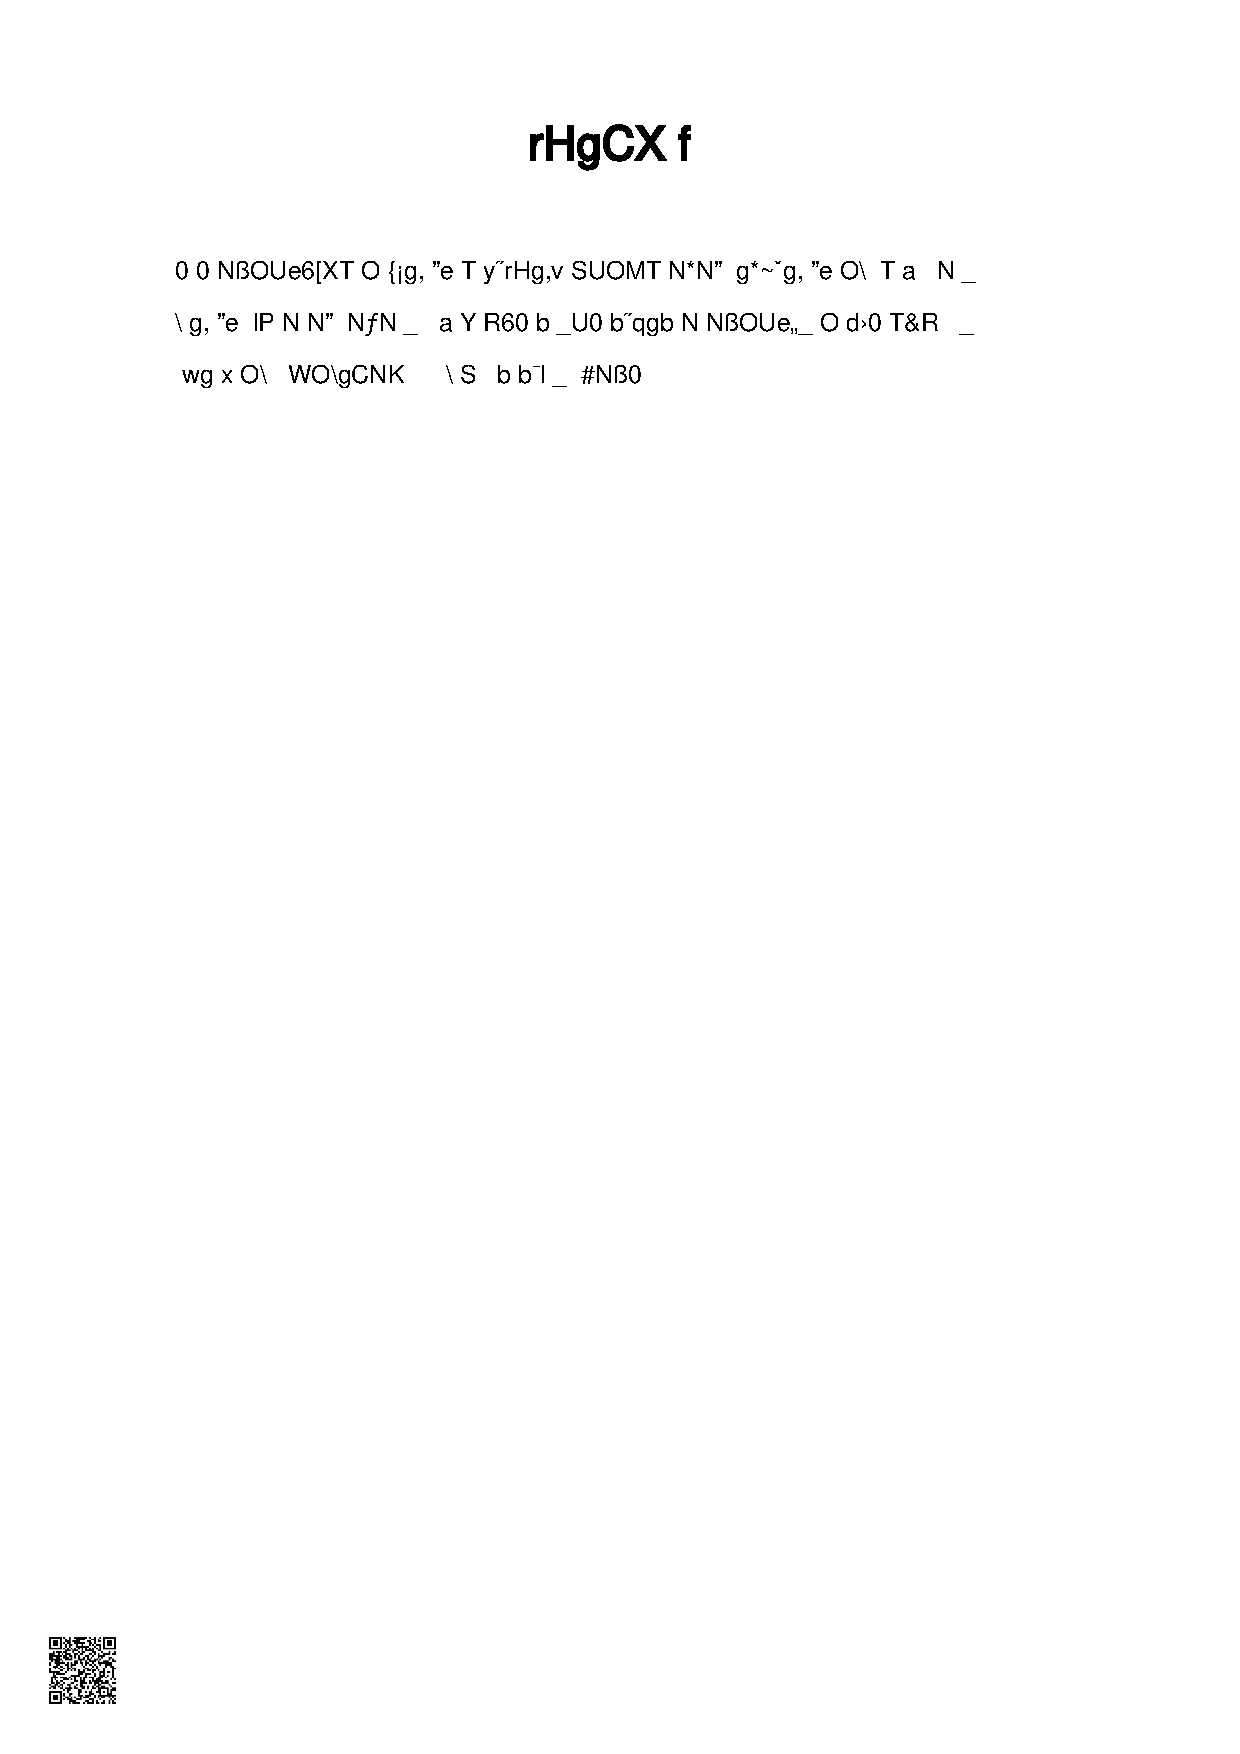
\includegraphics[height = 1.2448\textheight]{img/bqsm_180xxxxxxx.pdf}
    }
\end{textblock}

% vim:ts=4:sw=4
    
    \cleardoublepage
    \pagestyle{plain}
    \setcounter{page}{0}
    \pagenumbering{Roman}
    \begin{cabstract}

% 距离人们观测到高能宇宙射线已经过了近百年的时间,时至今日这些宇宙射线的起源依然无法被准确地回答。中微子是一种不带电且相互作用微弱的基本粒子,它可以通过强子过程伴随宇宙线同时产生。通过寻找中微子的方式能够一锤定音地确定宇宙线的起源。
高能中微子是人们观测宇宙的重要信使,通过寻找高能中微子的天体物理源,我们可以更深入地理解天体物理加速机制,解答宇宙射线起源的百年难题。
建成于2010年12月的IceCube是世界上第一台立方公里级别的中微子望远镜,它首次观测到了来自宇宙中弥散的中微子流强。在随后的运行中,IceCube以3.5$\sigma$和4.2$\sigma$的置信度分别找到了可能的中微子源TXS-0506+056和NGC 1068。
IceCube的观测结果表明下一代中微子望远镜需要拥有更庞大的体积和更好的角度分辨率才能从弥散的中微子流强中确切地找到产生它的天体物理源。

海铃计划旨在中国南海建设一个新一代的中微子望远镜——海铃中微子望远镜(TRIDENT)。
本文的研究工作围绕海铃中微子望远镜的预研展开,主要分为四个部分:(1)中微子望远镜的模拟框架开发;(2)海铃的性能分析;(3)优化海铃的设计;(4)海铃探路者实验。

我们参与研发最新的CORSIKA8模拟程序,并以之为框架搭建了一套新的中微子事件产生器,在其中我们实现了中微子反应事件的重要性采样,以及调用现有的成熟物理模块进行深度非弹性散射,轻子传播能损和陶子衰变等物理过程的模拟。
得到反应的产物粒子后,我们会在阵列范围内对粒子进行高精度的模拟。为解决过程中的计算资源消耗问题,我们选择只用Geant4来追踪复杂的强子成分,而转用参数化的方式取代了电磁簇射模拟,以此获得了约$10^3$倍的性能提升。
这些能够产生切伦科夫光的带电粒子径迹随后会被输入到一个我们自己开发的GPU加速的光线追踪模拟程序中。程序会利用GPU的并行计算功能,可以达到每秒处理$4\times 10^8$个光子的处理速度,相比于传统模拟提升约有$10^3$倍。
在光子到达混合数字光学模块(hDOM)表面后,我们使用Geant4来模拟光子传播到光敏元件——光电倍增管(PMT)和硅光电倍增器(SiPM)的行为。在此程序中,hDOM内部的几何细节都被清晰得构建出来。
此外,我们还设计了模拟PMT将到达其表面的光子放大成电信号波形的程序。

我们使用自己构建的模拟程序进行了大批量的中微子事件模拟,用于分析海铃中微子望远镜的性能。
我们对缪子中微子($\nu_\mu$)产生的径迹型事件进行了角度重建分析,基于hDOM测量到的光子到达时间,我们使用最大似然估计的方法来重建径迹的方向。我们的重建结果表明海铃对$1\,\mathrm{TeV}$的$\nu_\mu$的角度分辨率可以达到$1^\circ$以内,而对$100\,\mathrm{TeV}$的$\nu_\mu$可以达到约$0.1^\circ$。
我们对海铃中$\nu_\mu$的有效面积进行了分析,通过对事件完备的采样和筛选,我们得到海铃在$10\,\mathrm{TeV}$处有$\sim 10^2\,\mathrm{m^2}$的有效面积,并在$1\,\mathrm{PeV}$处达到$2 \times 10^3\,\mathrm{m^2}$。
利用角分辨和有效面积,我们可以分析海铃对中微子点源的灵敏度,我们发现海铃能够在一年内就以$5\sigma$的置信度发现NGC 1068。
而且海铃靠近赤道的纬度位置使它的灵敏观测带随着地球的自转扫描整个天空,实现对银心等区域的高灵敏度观测,补全IceCube对南天的观测空缺。

利用上述搭建起来的模拟和分析流程,我们可以对中微子望远镜中的设计进行优化。
我们探讨了相比于传统只含有PMT的mDOM,加入了SiPM之后的hDOM在径迹型事件的方向重建上的优势。我们发现SiPM的快速时间响应性能和高量子效率能够带来约$40\%$的角度重建精度的提升。
我们还对一种新的探测器几何构型——彭罗斯构型进行了研究。该构型参考自彭罗斯镶嵌,其中夹杂着密集和稀疏的区域,用以拓宽对簇射型事件的响应能区。此外,阵列的非周期性排布也能有效降低径迹型事件漏过探测器。
最后,我们研究望远镜的性能随着阵列中hDOM之间的水平和垂直方向上的间距的变化。
我们尝试了多种不同的间距缩放因子,发现将水平间距和垂直间距放大到1.2倍有利于探测能谱指数为-2的源;而当前的几何配置对于探测能谱指数为-3的中微子源已经是相对优秀的了。

除了上述模拟和分析的研究外,我们还进行了海铃探路者实验。该实验于2021年9月在海铃选址——南海西沙群岛附近海域成功开展,将自主研发设计的PMT测量系统和相机测量系统布放到$3400\,\mathrm{m}$深实现了原位的海水的光学性质。
我所在的小组几乎从零开始完成了对PMT系统的整体设计,PMT性能测试,系统响应标定,水下实验采数,以及后续数据分析的全套流程。我们还开发了与之配套的模拟程序,用以定量地分析吸收和散射的效应,辅助实验设计和数据分析。

探路者实验中测量得到的海底海洋地质数据以及海水光学性质验证了预选海域为理想的中微子望远镜台址。
当下,“海铃计划一期”项目已经启动,与之对应的预研工作正在进行中,我们预期在2026年建成具有10根串列单元的阵列,成为世界首个近赤道的中微子望远镜。

\end{cabstract}

\begin{eabstract}

High-energy neutrinos are important messengers to observe the universe. By searching for the astrophysical sources of high-energy neutrinos, we can understand of acceleration mechanisms in the extreme astrophysical sources and solve the century-old mystery of the origin of cosmic rays.
IceCube, built in December 2010, is the world's first kilometer-scale neutrino telescope. It first observed a diffuse neutrino flux of from the universe. In subsequent operations, IceCube found potential neutrino sources TXS-0506+056 and NGC 1068 with confidence levels of 3.5$\sigma$ and 4.2$\sigma$, respectively.
The observation results from IceCube suggest that the next generation of neutrino telescopes need a larger volume and better angular resolution to identify the astrophysical sources that produce the diffuse neutrino flux.

The Hai Ling Project aims to construct a next-generation neutrino telescope, TRIDENT, in the South China Sea. This paper focuses on the pre-research of TRIDENT and is divided into four main parts: (1) the development of the simulation framework for the neutrino telescope, (2) performance analysis of TRIDENT, (3) optimization of the design of TRIDENT, and (4) the TRIDENT Pathfinder experiment.

We participated in the development of the latest simulation program - CORSIKA8 and used it as a framework to build a new neutrino event generator. We implemented important sampling of neutrino events in this generator and it can call mature physics modules such as Pythia8, PROPOSAL, and TAUOLA for simulating deep inelastic scattering, lepton energy loss during propagation, and tau decay, and so on.
After obtaining the interaction products, we perform high-precision simulations for particles that arrive at the array. To address the issue of computational resource consumption, we choose to use Geant4 only to track complex hadronic interaction and replaced electromagnetic shower simulations with a parameterization method, which brings about a $10^3$ performance improvement.
The charged particle trajectories that can produce Cherenkov light are then input into a GPU-accelerated ray-tracing simulation program that we developed. This program utilizes the parallel computing capabilities of GPUs and can process $4 \times 10^8$ photons per second, which is about a $10^3$ improvement compared to traditional simulations.
After the photons reach the surface of the hybrid digital optical module (hDOM), we use Geant4 to simulate their behavior as they propagate to the photosensitive components such as photomultiplier tubes (PMTs) and silicon photomultipliers (SiPMs). In this program, the details of the internal geometry structure of the hDOM are crafted accurately.
Additionally, we have designed a program to simulate the amplification of photons reaching the surface of a PMT into electrical signal waveforms.

We simulated a large number of neutrino events using the simulation framework developed above to analyze the performance of the TRIDENT neutrino telescope. We performed angle reconstruction on track-type events produced by muon neutrinos ($\nu_\mu$). Based on the photon arrival time measured by hDOM, a maximum likelihood estimation method is used to reconstruct the direction of the track. Our reconstruction results showed that TRIDENT can achieve an angular resolution of less than $1^\circ$ for $\nu_\mu$ with an energy of $1,\mathrm{TeV}$, and $\sim 0.1^\circ$ for $100,\mathrm{TeV}$ $\nu_\mu$.
We analyzed the effective area of TRIDENT for $\nu_\mu$. We simulated a complete event samples and select the well-reconstructed events. We found that TRIDENT has an effective area of $\sim 10^2,\mathrm{m^2}$ at $10,\mathrm{TeV}$ and reaches $2\times 10^3,\mathrm{m^2}$ at $1,\mathrm{PeV}$, which is more than ten times that of IceCube.
Using the angular resolution and effective area, we analyzed the sensitivity of TRIDENT to neutrino point sources. By analyzing the correlation of events in direction space, we found that TRIDENT can discover NGC 1068 with a confidence level of $5\sigma$ within just one year. 
TRIDENT also has the detection capability beyond IceCube-Gen2 for neutrino sources in all directions of the sky.
TRIDENT will observe the potential neutrino sources at Southern sky, such as the Galactic Center, with unprecedented sensitivity.


Using the simulation and analysis framework we built, we studied the optimization of the design of the neutrino telescope.
We explored the advantage of using SiPMs in hDOM compared to the traditional mDOM with only PMTs for direction reconstruction of track-like events. In the study, we found that the fast timing ability and high quantum efficiency of SiPMs brings a 40\% improvement in angular resolution compared to mDOM.
We also studied a new detector geometry layout that follows Penrose tiling. This layout includes dense and sparse regions to expand the response energy range for shower-like events. Moreover, the non-periodic structure of the array can effectively reduce the corridor events that slip through the array.
Finally, we investigated how the performance of the telescope changes with the horizontal and vertical spacing between hDOMs in the array. We tried several different scaling factors and found that increasing the horizontal and vertical spacing by 1.2 times was beneficial for detecting sources with a spectral index of -2, while the current geometry is already optimized for sources with a spectral index of -3.

In addition to the aforementioned simulation and analysis studies, we also conducted a TRIDENT exploratory experiment. The experiment was successfully conducted in September 2021 in the vicinity of the Xisha Islands in the South China Sea, where our independently developed PMT measurement system and camera measurement system were deployed at a depth of 3400 meters to obtain in-situ optical properties of seawater.
Our research group completed the entire process of PMT system design, performance testing, system response calibration, underwater experimental data collection, and subsequent data analysis almost from scratch. We also developed a simulation program to quantitatively analyze the effects of absorption and scattering, which assisted in experimental design and data analysis.

The geological data of the seabed and the optical properties of seawater obtained from the exploratory experiment confirmed the pre-selected site as an ideal location for a neutrino telescope.
Currently, the TRIDENT Phase I project with 10 strings has been launched, and corresponding preliminary research is underway. We expect to build the world's first near-equatorial neutrino telescope in 2026.

\end{eabstract}

% vim:ts=4:sw=4

    \tableofcontents
    % 如有需要使用表格索引、插图索引
    % \listoftables
    % \listoffigures
    % 如有需要使用主要符号对照表
    % \begin{denotation}

\item[$x,y,m,n,t$] 标量,通常为变量
\item[$K,L,D,M,N,T$] 标量,通常为超参数
\item[$x\in \mathbb{R}^{D}$] D维列向量
\item[$(x_1,\cdots,x_D)$] D维行向量
\item[$(x_1,\cdots,x_D)^T$ or $(x_1;\cdots;x_D)^T$]  D维行向量
\item[$\v A\in \mathbb{R}^{K\times D}$]  大小为$K\times D$的矩阵
\item[$x\in \mathbb{R}^{KD}$]  ($KD$)维的向量
\item[$\mathbb{M}_i$ or $\mathbb{M}_i(\v x)$]  第$i$列为$\v 1$(或者$\v x$),其余为$\v 0$的矩阵
\item[$diag(\v x)$]  对角矩阵,其对角元素为$\v x$
\item[$\v I_N$ or $I$]  ($N\times N$)的单位阵
\item[$diag(\v A)$]  列向量,其元素为$\v A$的对角元素
\item[$\v A \in \mathbb{R}^{D_1\times D_2\times \cdots \times D_K}$]  大小为$D_1\times D_2\times \cdots \times D_K$的张量
\item[$\{x^{(n)}\}^{N}_{n=1}$]  集合
\item[$\{(x^{(n)},y^{(n)})\}^{N}_{n=1}$]  数据集
\item[$\mathcal{N}(\v x;\mu,\sum)$]  变量$x$服从均值为$\mu$,方差为$\sum$的高斯分布

\end{denotation}
    
    \mainmatter
    \chapter{引论}
\label{chap:introduction}

\section{中微子}

中微子是标准模型中的一种基本粒子\cite{Griffiths:2008}。它拥有$1/2$的自旋特征,是一种费米子。中微子不带电,而且质量非常小,约在eV量级。
自然界中存在三种味道的中微子——电子中微子$\nu_e$,缪子中微子$\nu_\mu$和陶中微子$\nu_\tau$,他们分别对应于三种不同代的轻子——电子$e$,缪子$\mu$和陶子$\tau$。
在四种基本的相互作用中,中微子只参与引力相互作用和弱相互作用。

中微子的概念最早由泡利于1930年提出,当时泡利试图引入这种不带电的新粒子来解释贝塔衰变实验中能量不守恒的问题。
随后费米正式提出了一套关于电弱相互作用的理论模型,即费米四顶点模型,其中便包含了泡利提出的不带电的新粒子。
如果这个新粒子的质量非常小,那么贝塔衰变中观测到的电子能谱便能够被非常完美地解释。
因此费米称这个新粒子为中微子(neutrino,在意大利语中意味着中性的微小粒子)。

自弱相互作用模型和中微子被提出以来,中微子便成为了粒子物理领域的一大研究热点。
1941年,我国核物理学家王淦昌首次提出了用贝塔捕获的方式来探测中微子\cite{Wang:1942}。
1956年, Clyde Cowan和Frederick Reines等人通过反贝塔衰变的方式首次真正探测到了中微子的存在\cite{Cowan:1956}。他们也因此在约40年后被授予1995年的诺贝尔物理学奖。

\begin{figure}[htb]
    \centering
    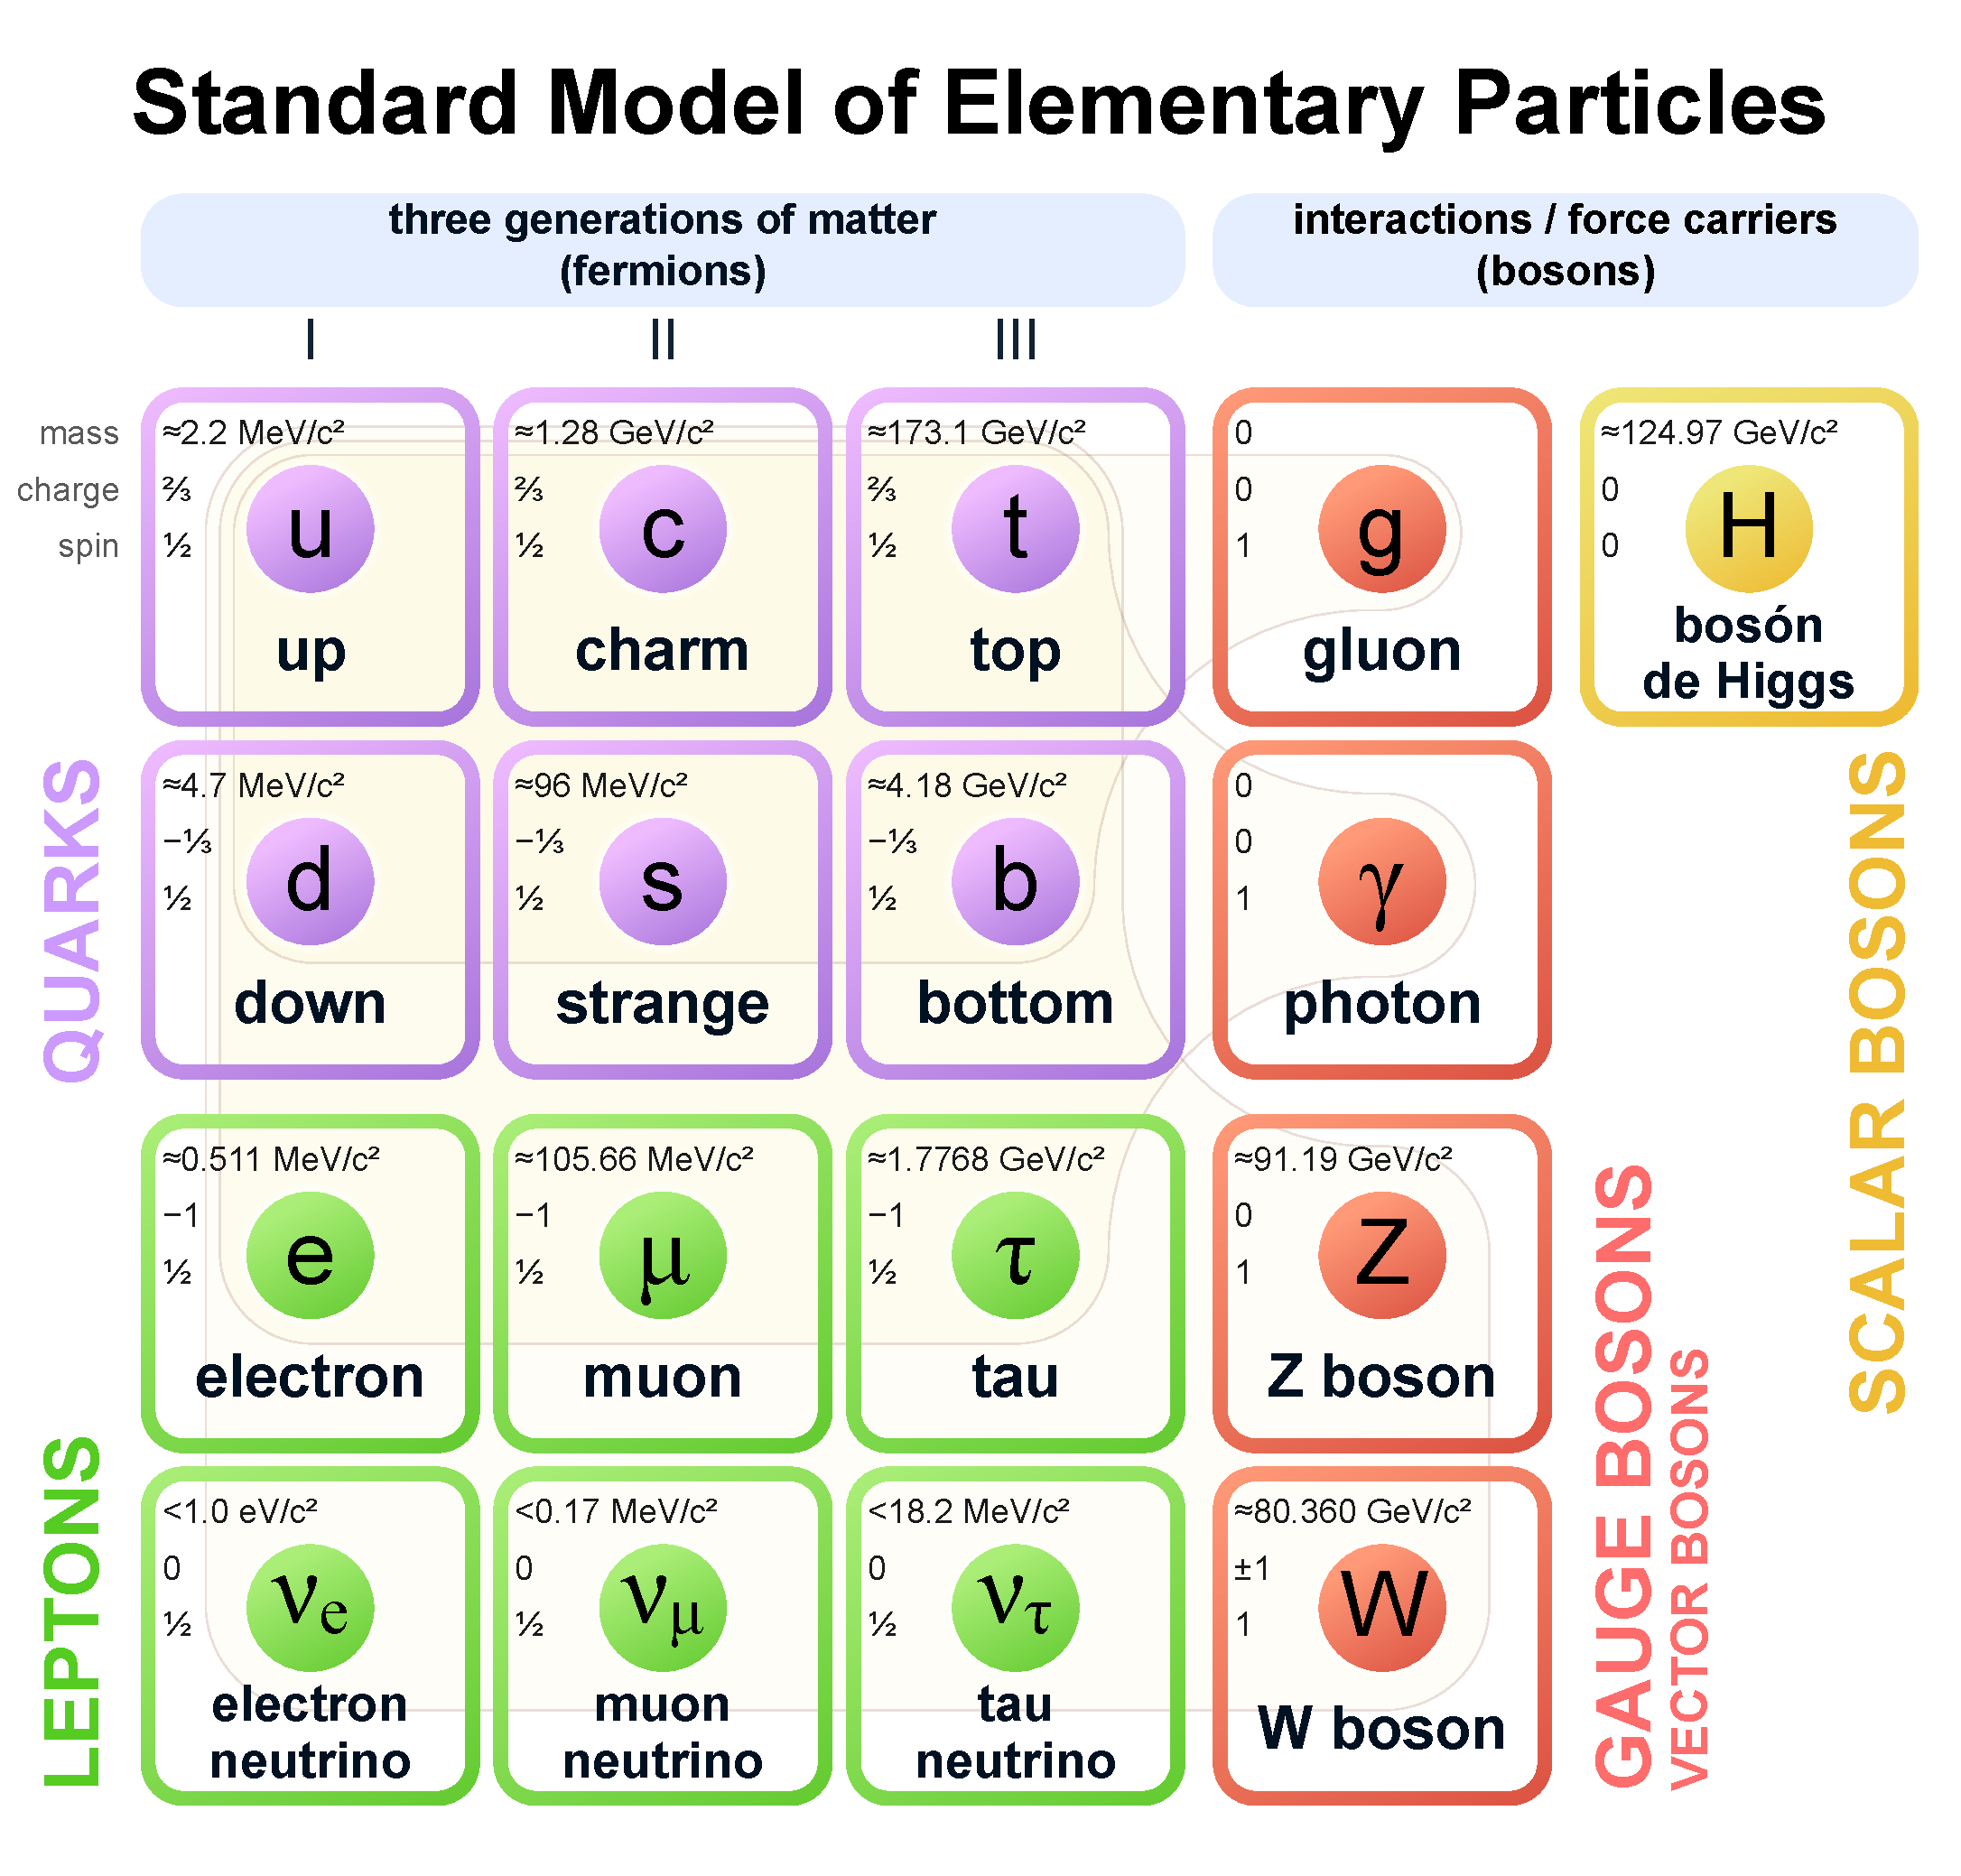
\includegraphics[width=0.8\linewidth]{img/standard_model.pdf}
    \caption{粒子物理标准模型中粒子以及假设的引力子。图片来自于维基百科}
    \label{fig:standard_model}
\end{figure}

\subsection{中微子振荡}

自19世纪50年代以来,Raymond Davis便已经在进行有关太阳中微子的探测\cite{Davis:1955}。在经过了数十年的实验后,他终于测到了太阳中微子,并因此获得了2002年的诺贝尔物理学奖。但与此同时,他在实验中也发现了太阳中微子的流量要低于理论预期值\cite{Cleveland:1998},这个问题被称为“太阳中微子缺失问题”。

中微子振荡模型可以用于解释“太阳中微子缺失问题”\cite{Bahcall:2001}。标准模型并没有限制中微子必须是无质量粒子,假如中微子存在质量的话,那么它的质量本征态($|\nu_k\rangle$,其中$k=1,2,3$),可以构成与味道本征态($ |\nu_\alpha\rangle$,其中$\alpha = e, \mu, \tau$)相互独立的一组量子态基矢,我们观测到的味道本征态的中微子可以是由不同的质量本征态的中微子相互组合后产生的:
\begin{equation}
    \left|v_{\alpha}\right\rangle = \sum_{k=1}^{3} U_{\alpha k}^{*}\left|v_{k}\right\rangle , 
    \label{eq: neutrino oscillation}
\end{equation}
其中$U$是一个幺正矩阵,被称作轻子混合矩阵,或者Pontecorvo-Maki-Nakagawa-Sakata (PMNS)矩阵\cite{Pontecorvo:1957, Maki:1962, Pontecorvo:1967}。它通常被分解成如下的形式:
\begin{equation}
    U=\left(\begin{array}{ccc}{1} & {0} & {0} \\ {0} & {c_{23}} & {s_{23}} \\ {0} & {-s_{23}} & {c_{23}}\end{array}\right)\left(\begin{array}{ccc}{c_{13}} & {0} & {s_{13} e^{-i \delta_{\mathrm{CP}}}} \\ {0} & {1} & {0} \\ {-s_{13} e^{i \delta_{\mathrm{CP}}}} & {0} & {c_{13}}\end{array}\right)\left(\begin{array}{ccc}{c_{12}} & {s_{12}} & {0} \\ {-s_{12}} & {c_{12}} & {0} \\ {0} & {0} & {1}\end{array}\right) P_\nu , 
    \label{eq: PMNS matrix}
\end{equation}
其中$c_{ij}$和$s_{ij}$分别表示中微子振荡角$\theta_{ij}$的余弦值和正弦值,$\delta$表示狄拉克CP对称性破坏相位角,而$P_\nu = \mathrm{Diag} \{e^{i\rho},  e^{i\sigma}, 1 \}$表示马约拉纳相位角并与中微子振荡现象无关。

中微子振荡现象最终在超极神冈(Super-Kamiokande)和Sudbury中微子观测站中得到了验证\cite{Super-K:1998, Sudbury:2001}。
中微子振荡被认为是人们发现的首个超出标准模型的物理现象。2015年的诺贝尔物理学奖授予Takaaki Kajita和Arthur B. McDonald,以此来表彰他们在中微子振荡中做出的贡献。


\subsection{无中微子双贝塔衰变}

马约拉纳粒子是一种反粒子便为自身的费米子。这种粒子的概念由Ettore Majorana于1937提出。
由于马约拉纳粒子必须不带有电荷,因而中微子便成为了标准模型框架下唯一可能的马约拉纳粒子。
假如中微子真的是马约拉纳粒子,那么它将破坏轻子守恒定律,而这通常是超出标准模型的新物理的特征。
然而中微子微小的质量使得我们难以确认它到底是狄拉克粒子还是马约拉纳粒子。

目前实验上确认中微子是否是马约拉纳粒子的唯一途径便是观测无中微子双贝塔衰变($0\nu\beta\beta$):
\begin{equation}
    N(A, Z) \rightarrow N(A, Z+2) +2 e^{-} ,
    \label{eq: double beta decay}
\end{equation}
其中$N(A, Z)$表示质子数和中子数都为偶数的原子核,且它的质量必须大于与之拥有同样中子数但大两个质子数的原子核$N(A, Z+2)$。满足该特征的原子核有$^{48}Ca$,$^{76}Ge$和$^{136}Xe$等。
目前已经有许多项正在进行和规划中的实验来探寻$0\nu\beta\beta$信号,例如:PandaX\cite{PandaX-II:2019},KamLAND-Zen\cite{KamLAND-Zen:2016},EXO-200\cite{EXO-200:2012}等等。$0\nu\beta\beta$实验被认为是寻找新物理的重要方向。


\section{高能中微子天文学}

由于具有不带电且相互作用微弱的性质,中微子可以穿越复杂的宇宙环境而到达地球,是一种观测宇宙的重要信使。用中微子来观测宇宙中的物理现象,这便是中微子天文学。
通过中微子信使,人们可以观测到天体中光子无法穿透的高密度区域。中微子天文学在粒子物理,天体物理以及宇宙学中都有重要的作用。
例如,太阳中微子的观测对于理解太阳内部的核反应过程和建立标准太阳模型有至关重要的作用\cite{Bahcall_solar_model:2005}。
在1987年,人们在银河系的卫星星系——大麦哲伦星云中发生的超新星爆发SN 1987a中探测到了中微子\cite{Hirata_sn:1987, Bionta_sn:1987}。这为超新星爆发模型提供了有力的支持,该模型认为超新星中的大部分能量都以中微子的形式释放了出去。
本文的主要研究对象为高能中微子(亚TeV-EeV能级),故在下文中我们主要讨论天体物理起源的高能中微子,并且在不做特殊说明的情况下,我们在后文中将高能中微子天文学简称为中微子天文学。

\subsection{高能宇宙线与中微子}

\subsubsection{高能宇宙线简介}

宇宙线是来自宇宙中的高能带电粒子,它的成分主要是质子和少量的氦核以及其他重核\cite{Gaisser:2016}。
宇宙线的能量可以跨越数个量级,从$\sim 10 \,\mathrm{GeV}$一直延续到$\sim 100 \,\mathrm{EeV}$,其高能段远远超过了人类目前制造的加速器所能加速能量的极限。
宇宙线的能谱如图\ref{fig:CR_spectrum}所示,呈现幂律谱的形式:在低能处数量较多,例如在$\sim 1 \,\mathrm{TeV}$处每平方米每秒就会有一个宇宙线粒子通过,而高能处事例数极少,例如在$\sim 100 \,\mathrm{PeV}$处大约每平方米每年才会有一个宇宙线粒子通过。
自上世纪30年代宇宙线被人类发现以来,人们通过宇宙线发现了大量新的粒子,例如$\pi$介子,缪子,K介子等。
尽管人们对宇宙射线的研究在近百年的时间内从未停止过,超高能宇宙线粒子的起源至今没有明确的答案。
这是由于宇宙线携带电荷,它在星际传播的过程中受到磁场的影响而改变其传播方向,因此人们在地球上难以从观测到的宇宙线追溯回它来源的天体。
相比之下,中微子不带电且相互作用微弱,探测与高能宇宙线同时产生的高能中微子将有助于解答高能宇宙线起源的百年难题。

\begin{figure}[htb]
    \centering
    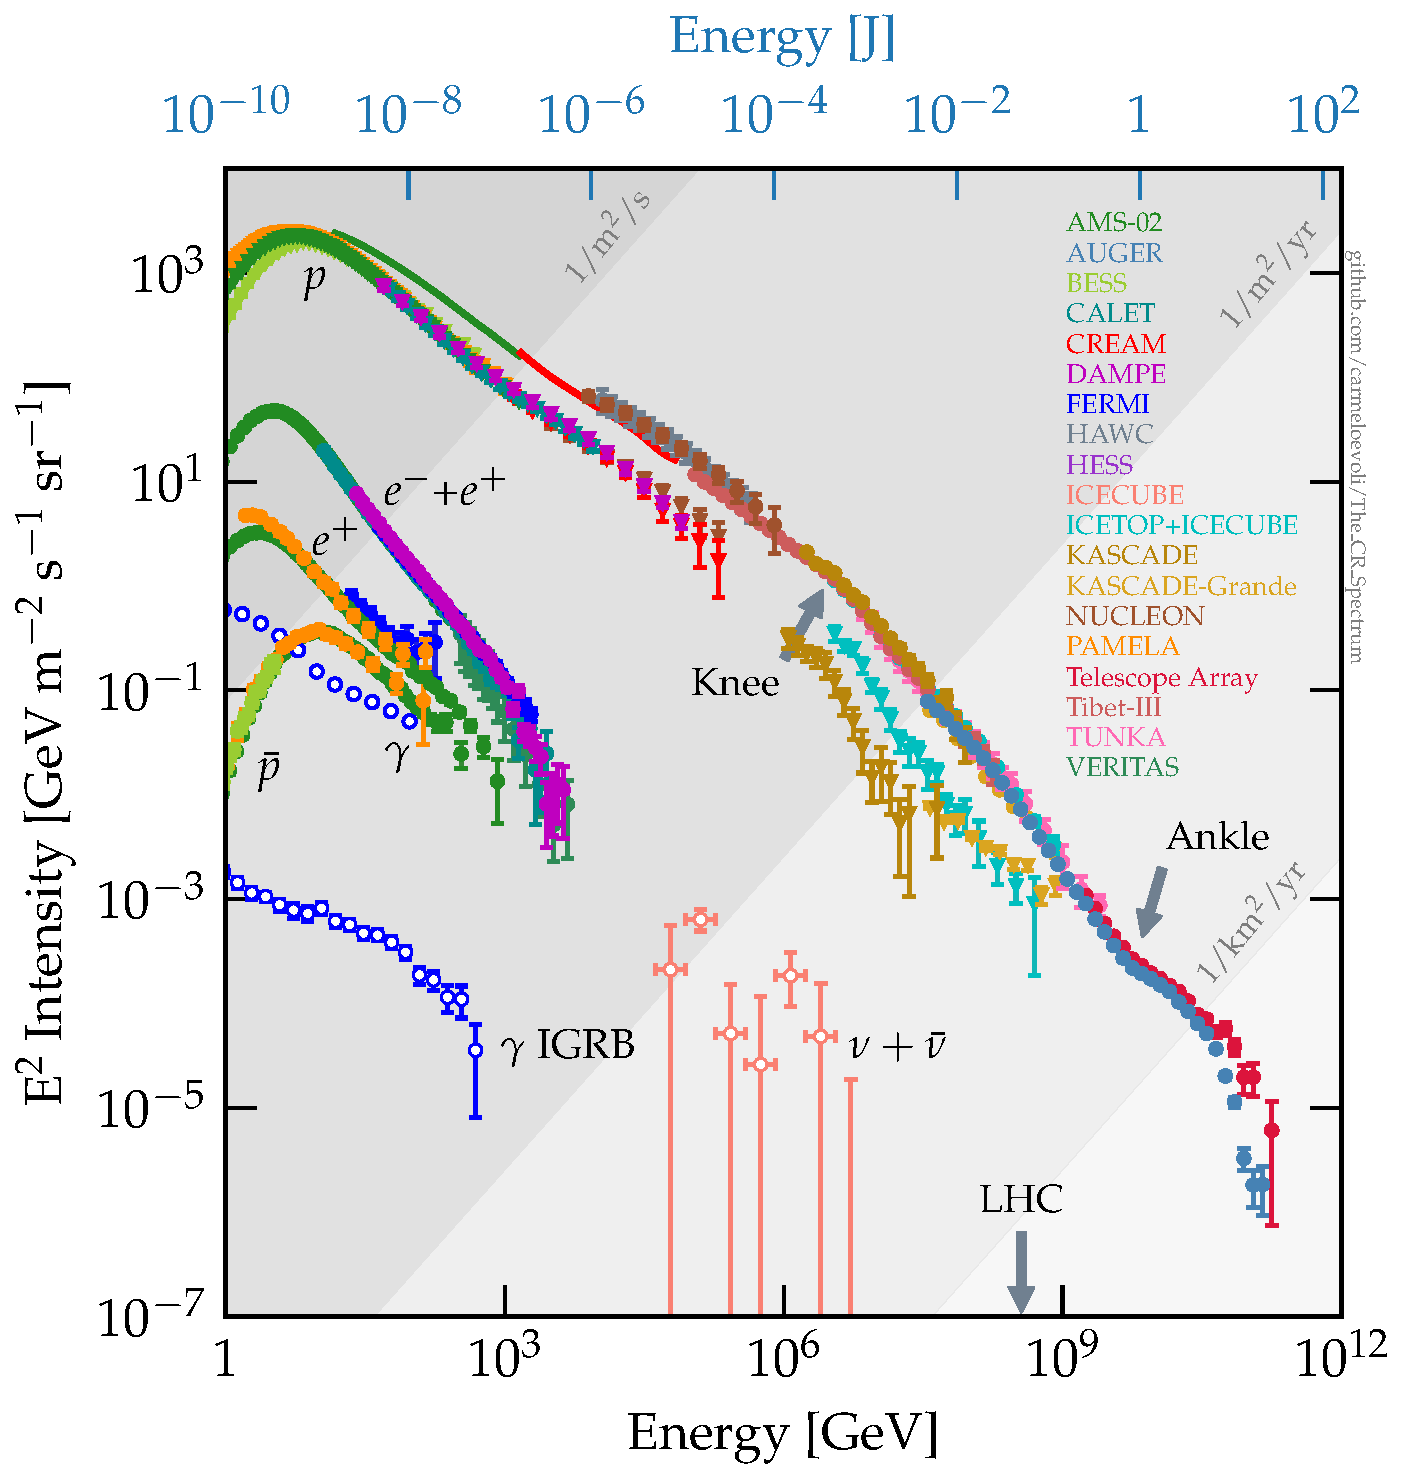
\includegraphics[width=0.8\linewidth]{img/cosmic_ray_spectrum.pdf}
    \caption{各个成分的宇宙线的流量随着能量的变化关系。图片来自\cite{CR_spectrum:2022}}
    \label{fig:CR_spectrum}
\end{figure}

\subsubsection{宇宙线加速机制}

宇宙线能谱的幂律形式可以用费米加速机制来解释。费米曾经提出了一种加速机制,即利用一团运动的磁云来多次使得粒子在其中来回地被磁场弯曲弹射\cite{Fermi_acceleration:1949},其物理图像如图\ref{fig:CR_acceration}中左图所示。
宇宙线粒子在每一次与磁云的碰撞过程(即受到磁云的磁场的作用而改变运动方向)中,粒子都会获得正比于自身初始能量的能量。因此,在经过多次碰撞后,粒子将获得极高的能量。
并且,粒子在每次碰撞过程中都有一定几率摆脱磁云的束缚而离开加速区,进而被地球的观测者所观测到。在这两种效应的结合下,最终观测者看到的粒子能谱会呈现出观测到的幂律谱的形式。

费米加速机制可以很好地解释观测到的幂律能谱,它在后续的几年中被不断地改进,并且应用到大量其他的天体物理环境中,其中最著名的便是扩散激波加速机制\cite{Bell_shock_1:1978, Bell_shock_2:1978},其图像如图\ref{fig:CR_acceration}中右图所示。
在扩散激波加速机制中,粒子每次碰撞所获得的能量正比于激波速度$v/c$的一次方,而非原始费米加速机制下的二次方,因而具有更高的加速效率。根据加速过程中获得能量与激波速度的幂律关系,扩散激波加速机制也被称为一阶费米加速机制,而通过磁云碰撞的加速机制则被称为二阶费米加速机制。

\begin{figure}[htb]
    \centering
    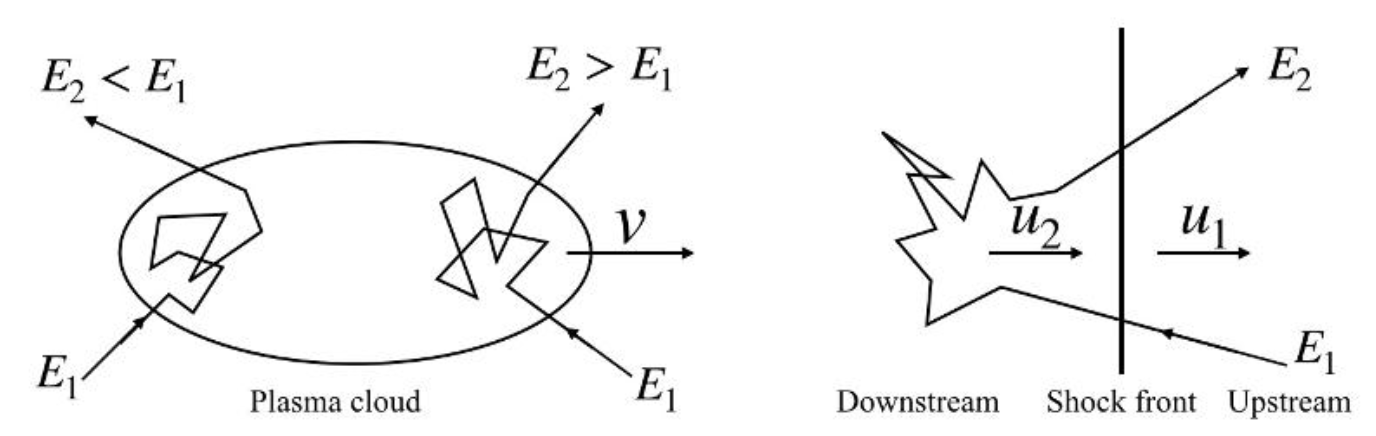
\includegraphics[width=0.8\linewidth]{img/Fermi_acceleration.png}
    \caption{宇宙线加速的模型。左图:费米二阶加速机制。宇宙线粒子与等离子体磁云碰撞而获得能量;右图:费米一阶加速机制,等离子体来回穿过激波上下游而获得能量。图片来自\cite{Gaisser:2016}}
    \label{fig:CR_acceration}
\end{figure}

在天体物理环境下,磁场的能量密度通常比较高,因此磁场可以使得带电粒子被束缚在加速区域中,从而有可能通过多次发生碰撞的形式得到加速。在这种图像下,带电粒子的能量不应过高,否则其回旋半径将会超过加速区的大小从而离开。磁场束缚下带电粒子加速的能量极限$E_\mathrm{Hillas}$被称为Hillas极限\cite{Hillas_limit:1984}:
\begin{equation}
    E_\mathrm{Hillas} = Z e c B R ,
\end{equation}
其中$Z$为带电粒子电荷数,$e$为元电荷量,$c$为光速,$B$和$R$分别为加速区的磁场大小和半径大小。

目前我们已经观测到$\sim 100\,\mathrm{EeV}$的宇宙线,即便是如此高的能量,依然有许多天体物理源的环境能够满足Hillas条件\ref{fig:Hillas_limit}。
他们中有的是具有极端的磁场环境,例如磁性,脉冲星和白矮星;有的是具有天体物理尺度的体积,例如射电星系和星系团。
对高能天体中微子的探测能够帮助我们定位究竟是何种天体源能够将粒子加速到如此高的能量,从而为理解具体的天体物理现象和宇宙线加速机制提供帮助。

\begin{figure}[htb]
    \centering
    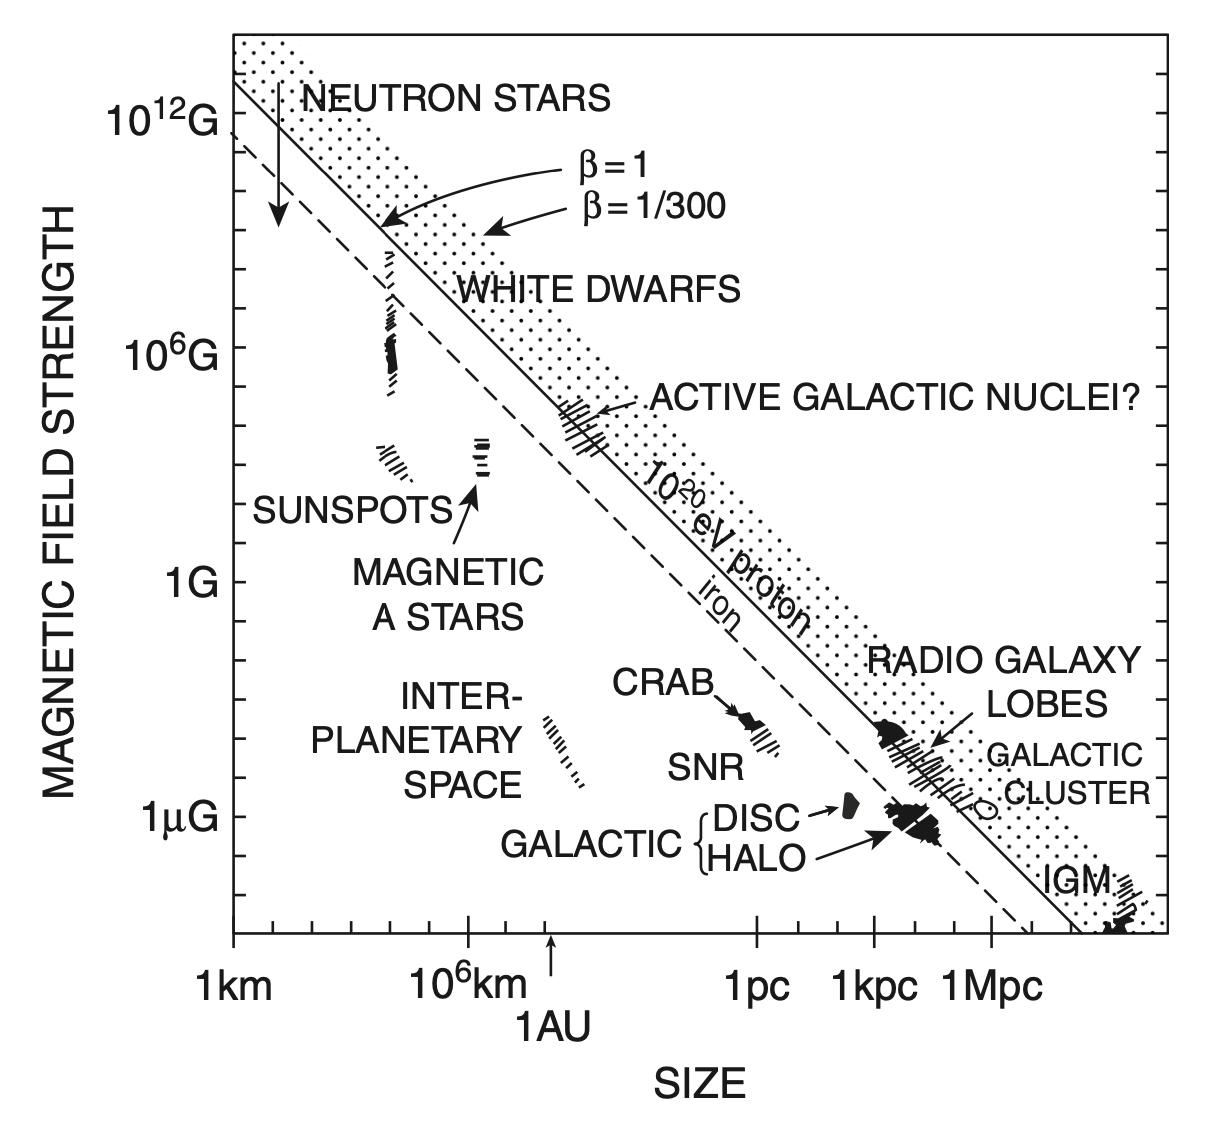
\includegraphics[width=0.8\linewidth]{img/Hillas_limit.png}
    \caption{潜在的宇宙线起源天体以及它们的大小和磁场强度。源的大小与磁场强度的乘积决定了源能加速的宇宙线的上限,即Hillas条件。图片来自\cite{Gaisser:2016}}
    \label{fig:Hillas_limit}
\end{figure}

\subsubsection{高能中微子产生机制}
\label{subsubsec:neutrino_production}

由于中微子不带电荷,故中微子自身难以被加速。在天体物理环境下,高能中微子主要由高能宇宙线粒子与其他粒子碰撞产生。
宇宙线粒子和重子背景或者光子背景碰撞,产生$\pi$介子,$K$介子等次级粒子,这些次级粒子通过衰变产生中微子。

以宇宙线中的质子为例,$pp$过程中质子与质子的非弹性散射表达式如下:
\begin{equation}
    p+p \rightarrow M_{p p}^{+} \pi^{+}+M_{p p}^{-} \pi^{-}+M_{p p}^0 \pi^0 + X ,
    \label{eq:pp_interaction}
\end{equation}
其中$M_{p p}^{+}: M_{p p}^{-}: M_{p p}^0 \approx 1: 1: 1$表示反应中产生的$\pi^{+}$,$\pi^{-}$和$\pi^{0}$粒子的数量,$X$表示其他更高阶的强子产物,例如$K$介子和$\Lambda$介子等。

另外一种反应通道——$p\gamma$过程中质子与光子的共振散射表达式如下:
\begin{equation}
    p+\gamma \rightarrow \Delta^{+} 
    \rightarrow\left\{
    \begin{array}{l}
        n+\pi^{+} \\
        p+\pi^0
    \end{array}
    \right. ,
    \label{eq:pgamma_interaction}
\end{equation}
其中$\Delta^{+}$是质子的共振态,拥有更高的质量和自旋,它会快速地通过强相互作用衰变为强子和$\pi$介子,衰变为中子和质子的几率比为$1/3 : 2/3$。

无论是$pp$过程还是$p\gamma$过程,单个产生的$\pi$介子从初始的高能质子中继承来的能量比例都约为:
\begin{equation}
    x_\pi = \left \langle \frac{E_\pi}{E_p} \right \rangle \simeq 0.2 ,
\end{equation}
其中$E_p$是高能质子的能量,$E_\pi$是反应产生的$\pi$介子的能量。

以上两种反应中产生的$\pi$介子会继续通过电弱相互作用衰变,产生中微子和光子:
\begin{equation}
    \begin{aligned}
        & \pi^{+} \rightarrow \mu^{+}+v_\mu \rightarrow e^{+}+v_e+\bar{v}_\mu+v_\mu \\
        & \pi^{-} \rightarrow \mu^{-}+\bar{v}_\mu \rightarrow e^{-}+\bar{v}_e+v_\mu+\bar{v}_\mu \\
        & \pi^0 \rightarrow 2 \gamma ,
        \label{eq:pion_decay}
    \end{aligned}
\end{equation}
在衰变过程中,我们可以近似地认为衰变产生的2个伽马光子各自携带$\pi$介子$1/2$的能量,4个轻子各自携带$\pi$介子$1/4$的能量。
因此最终反应得到的中微子的能量约为初始质子能量的$5\%$,光子的能量约为初始质子能量的$10\%$。

值得注意的是,由于缪子的寿命($2.2\,\mathrm{\mu s}$)要远远大于$\pi$介子的寿命($26\,\mathrm{ns}$),在部分强磁场的天体物理环境下,缪子可能会经历显著的能损过程,导致最终发生衰变时,其能量已经远低于初始能量,故缪子衰变得到的中微子可以忽略不计\cite{muon_damp:2005}。
在这种情况下,天体物理源处的各个中微子味道的比例将会从公式\ref{eq:pion_decay}中所描述的$v_e: v_\mu: v_\tau \approx 1: 2: 0$转变为$v_e: v_\mu: v_\tau \approx 0: 1: 0$。

目前对弥散的宇宙线流量,中微子流量,和伽马光子流量的观测如图\ref{fig:diffuse_neutrino_CR_gamma}所示,三种不同的信使之间存在着能量区间和流量大小的差异。
我们可以看到弥散伽马射线在高能处存在截断,这是由于极高能($\gtrsim 1\,\mathrm{TeV}$)的光子可以与星系间的背景光子场发生作用而产生正负电子对,因此宇宙对极高能的光子是不透明的。
宇宙线只画了GeV到EeV的能级,这是因为更低能量的宇宙线粒子在星际间磁场的作用下,其运动行为接近随机游走,已经彻底丧失了方向性。而更高能处宇宙线粒子的流量截断是由GZK效应,即宇宙线与宇宙微波背景辐射相作用导致的\cite{GZK_G:1966, GZK_ZK:1966}。

\begin{figure}[htb]
    \centering
    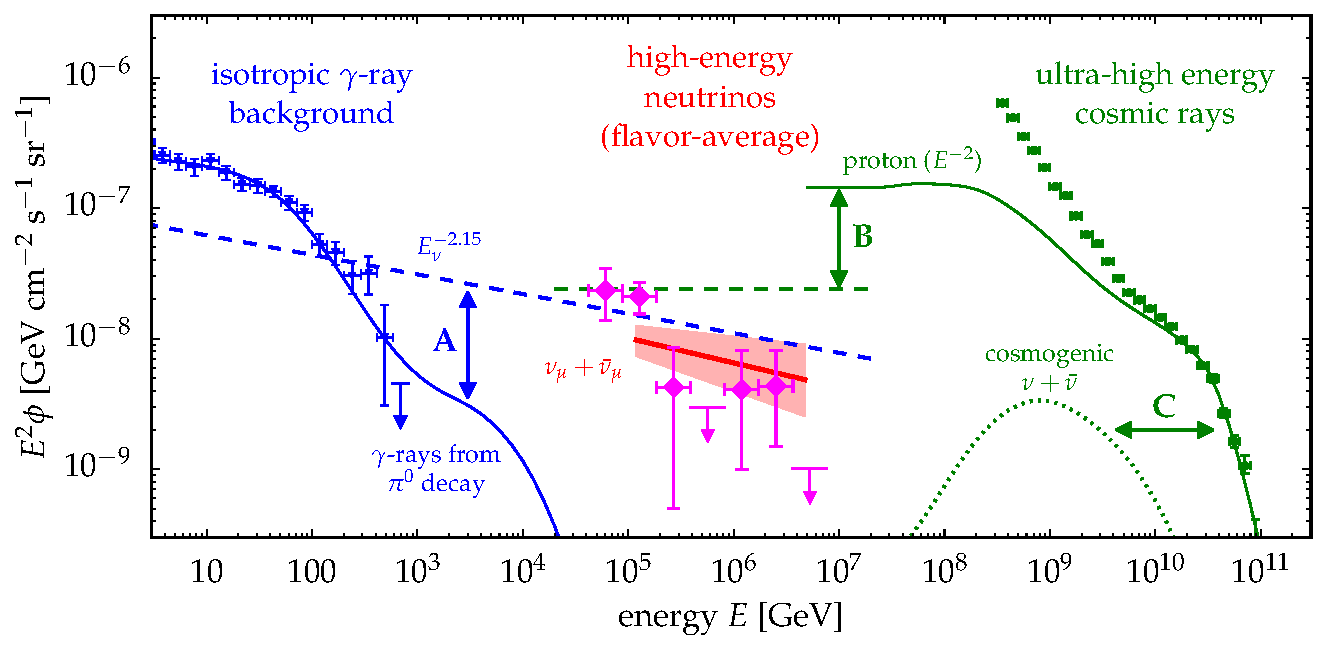
\includegraphics[width=0.8\linewidth]{img/diffuse_neutrino_CR_gamma.pdf}
    \caption{IceCube观测到的弥散中微子能谱(红色线表示缪子径迹事件的分析结果\cite{IceCube_diffse_muon:2017},粉色数据点表示高能起始事件的分析结果\cite{IceCube_6yr_cascade_spectrum:2017}),Fermi-LAT观测到的弥散的银河外伽马射线能谱(蓝色数据点)\cite{Fermi_diffuse_gamma:2014},以及Auger观测到的极高能宇宙线能谱(绿色数据点)\cite{Auger_diffuse:2015}。图片来自\cite{Astro2020_neutrino}}
    \label{fig:diffuse_neutrino_CR_gamma}
\end{figure}


\subsection{天体中微子源}

宇宙中有许多剧烈活动的天体,它们中有的已经被观察到了强烈的伽马射线辐射,表明他们具备加速宇宙线粒子的能力。
这些天体在加速宇宙线的过程中,如果能够将质子加速到超过PeV能级,并且在加速区域附件的背景场中存在足够多的气体或者光子成分,那么便有可能产生高能的中微子辐射。
在下面内容中,我们列举一些有潜力的高能中微子的天体源,如果想要了解更详细的研究,读者可以参考最近的综述\cite{Kurahashi_review_nu_mm:2022}。这些天体源有的是灾变型事件,具有比较短的活动时间,因而被称为暂现源,有的可以在上千年的时间中稳定地产生中微子,因而被称为持续源。

\subsubsection{暂现源}

伽马射线暴(Gamma Ray Burst,GRB)是自宇宙大爆炸之后最剧烈的天体活动之一,它能够在$\sim 1\,\mathrm{s}$的时间尺度上释放出$10^{51}-10^{53}\,\mathrm{erg}$能量的光子\cite{zhang:2018}。宇宙中的GRB事件所释放出来的能量足以产生我们所观测到的极高能宇宙线流量,是非常有潜力的极高能宇宙线的起源天体\cite{Waxman:1995}。此外,MAGIC和LHAASO分别在GRB 190114C和GRB 221009A中观测到了高达TeV能级的伽马光子\cite{MAGIC_GRB190114C:2019},证实了其高效的加速粒子能力。因此,GRB一直以来都被认为是非常有潜力的中微子源\cite{Waxman:1997ti}。

潮汐瓦解事件(Tidal Disruption Event,TDE)是恒星被超大质量黑洞吞噬时产生的事件。观测和数值模拟表明,TDE中可能包含有吸积盘,半相对论性的物质流出(outflow),以及可能包含一个喷流(jet)\cite{Dai_TDE:2018}。物质流出和喷流的结构可以将强子加速到高能,而吸积盘则可以提供背景光子场,因此TDE具备产生高能中微子的潜力\cite{Wu_TDE:2021, Zheng_TDE:2022, Winter_TDE:2022}。

\subsubsection{持续源}

脉冲星风星云(Pulsar Wind Nebulae,PWN)是由中子星向外发射的相对论性的星风与周围的介质相互作用产生的结构\cite{Mitchell_PWN:2022}。
PWN可以产生从射电到伽马射线的广谱辐射,最近LHAASO的观测表明脉冲星风星云可以产生PeV能量的伽马光子辐射\cite{LHAASO_Crab:2021},预示着PWN有能力将带电粒子加速到大于PeV的能量。

星爆星系(starburst galaxy)是指存在着高密度的气体,恒星形成活跃的星系。星爆星系中大质量恒星晚期的灾变事件发生频繁,具有充足的宇宙线供应。而且恒星会产生较强的磁场环境,将宇宙线束缚在其中,导致$\lesssim 1\,\mathrm{PeV}$的宇宙线与气体碰撞的时标要短于逃离时标,因此具备产生高能的弥散中微子流的潜力\cite{Loeb_starburst_galaxy:2006}。

活动星系核(Active Galactic Nuclei,AGN)是一个正在吸积物质的星系中心超大质量黑洞,在黑洞的附近存在着很强的紫外射线和X射线的辐射场。黑洞吸积盘中的物质在落入黑洞时,可能会和光子场发生作用,从而通过$p\gamma$过程产生中微子辐射\cite{Meszaros_AGN:2004, Murase_AGN:2015, Murase_AGN:2022, Murase_hidden_AGN:2022}。


\subsection{IceCube观测结果}

IceCube是目前世界上正在运行中的最大的中微子望远镜,它取得了丰富的观测结果。IceCube于2013年首次发现了来自宇宙中的高能中微子存在的证据\cite{IceCube_astro_neutrino_flux:2013}。2014年,IceCube又以$5.4\sigma$的置信度确认了它的存在\cite{IceCube_astro_neutrino_flux_3yr:2014},至此,IceCube宣布了高能天体物理中微子天文学的研究正式开始。

\subsubsection{弥散中微子能谱}

IceCube每年大约能观测到$\mathcal{O}(10)$个能量大于$100\,\mathrm{TeV}$的中微子事件。相比于大气缪子和大气中微子背景,这些高能的事件极有可能来自地球以外的宇宙空间中。
这些中微子事件在时间和空间上呈现出全天各向同性的分布,并没有明显地和已知的天体物理源成协。
通过对中微子事件进行筛选分析,IceCube测量出了弥散天体物理中微子能谱\cite{IceCube_6yr_cascade_spectrum:2020, IceCube_HESE:2020, IceCube_MESE:2014, IceCube_diffse_muon:2021, IceCube_starting_track:2021b}。不同分析的测量结果如图\ref{fig:IceCube_diffuse_spectrum}所示,图中的横坐标$\gamma_\mathrm{astro}$和纵坐标$\phi^{\nu_i+\bar{\nu}_i}_\mathrm{astro}$分别表示某一种味道的中微子能谱的谱指数和在$100\,\mathrm{TeV}$下的流量大小,即中微子能谱被表示为幂律谱的形式:
\begin{equation}
    \phi^{\nu_i+\bar{\nu}_i}_\mathrm{astro}(E_\nu) = \phi^{\nu_i+\bar{\nu}_i}_\mathrm{astro, 100\,TeV} \times \left( \frac{E_\nu}{100\,\mathrm{TeV}} \right)^{-\gamma_\mathrm{astro}} \times 10^{-18} \, \mathrm{s^{-1} cm^{-2} GeV^{-1} sr^{-1}}
    \label{eq:diffse_nu_flux}
\end{equation}

我们可以看到在图\ref{fig:IceCube_diffuse_spectrum}中,不同的筛选条件得到的样本的能谱略有差异,由能量阈值最低的来自北天的径迹型事件\cite{IceCube_diffse_muon:2021}测量得到的能谱比较硬,能量阈值中等的簇射型事件\cite{IceCube_MESE:2014, IceCube_6yr_cascade_spectrum:2020}测出的能谱比较软,而高能簇射型事件\cite{IceCube_HESE:2020}得到的能谱最软,其值接近-3。
这可能预示着中微子的能谱从低能到高能可能存在着由硬逐渐变软的过程,而并非一个单一的幂律谱。

\begin{figure}[htbp]
    \centering
    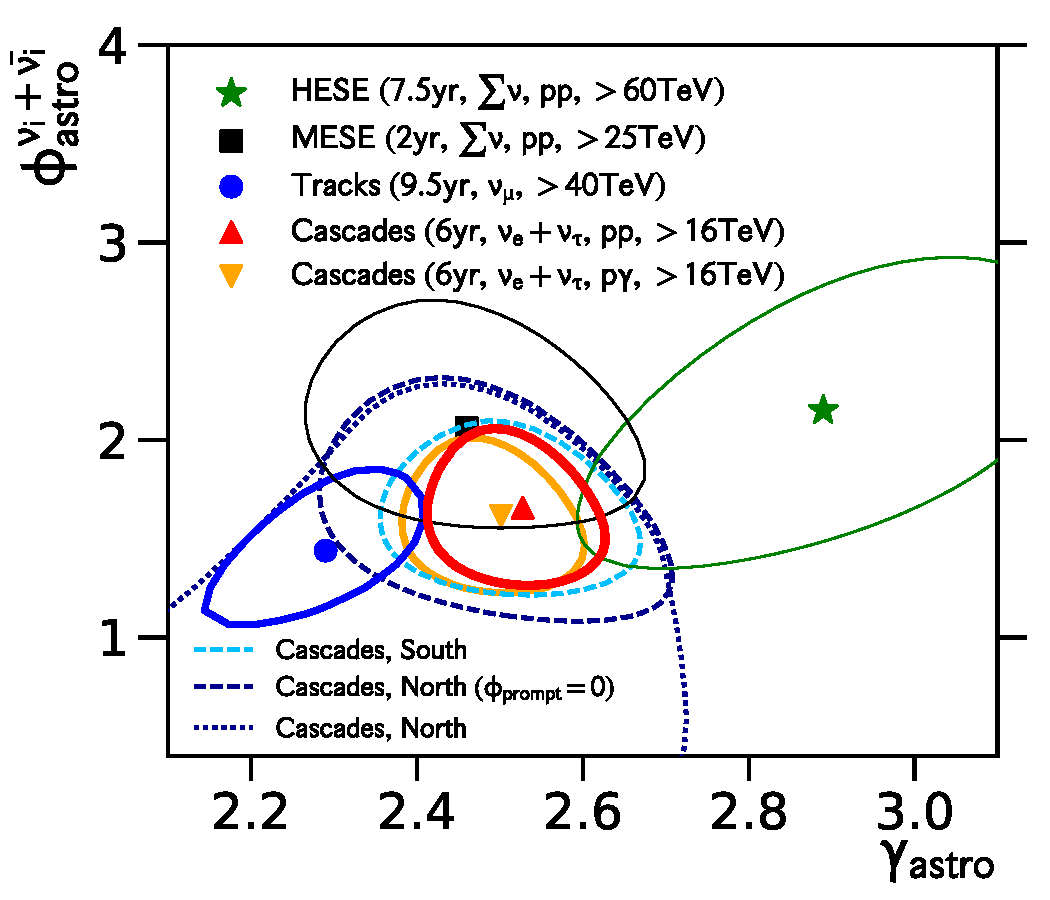
\includegraphics[width=0.6\linewidth]{img/IceCube_diffuse_spectrum.pdf}
    \caption{IceCube筛选不同的数据集测量得到的弥散中微子能谱。图片来自\cite{IceCube_6yr_cascade_spectrum:2020}}
    \label{fig:IceCube_diffuse_spectrum}
\end{figure}

IceCube通过对弥散中微子流量的数据分析表明中微子源呈现出单个源流量弱而数量多的弥散特征,因此整体上源的搜寻比较困难。IceCube对源的密度和亮度的限制如图\ref{fig:neutrino_sources}所示。
这种数量弥散而亮度微弱的源要求下一代的中微子望远镜必须具备更好的角分辨率和有效面积,才能从弥散的流量中寻找到确切的中微子源\cite{Fang_resolve_flux:2016}。

\begin{figure}[htbp]
    \centering
    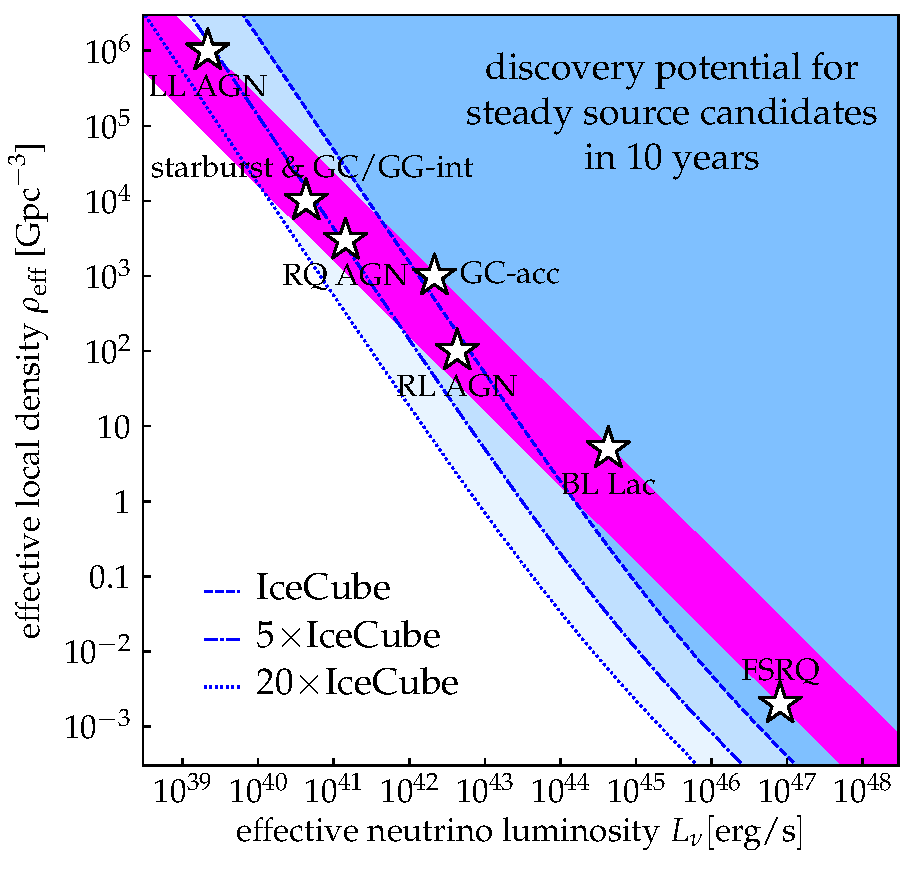
\includegraphics[width=0.45\linewidth]{img/sources_steady.pdf}
    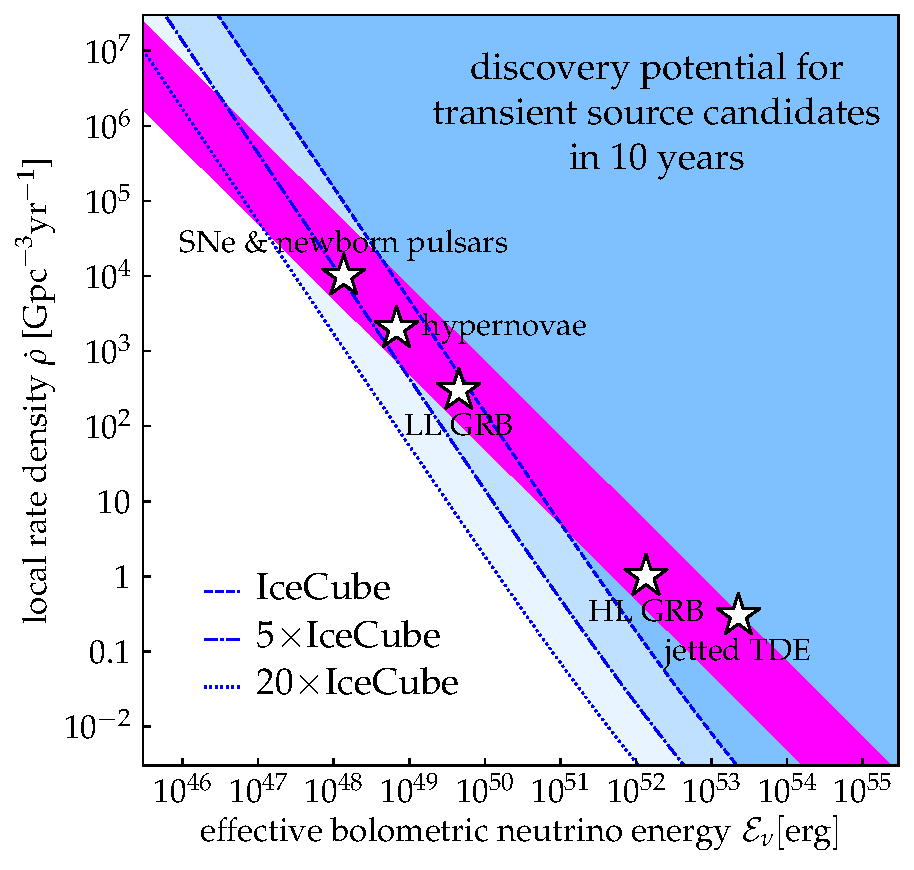
\includegraphics[width=0.45\linewidth]{img/sources_transient.pdf}
    \caption{IceCube观测对天体物理中微子源的限制。左侧:观测到的弥散中微子流量(洋红色带状区域)和天体物理源持续源的密度以及光度的关系。洋红色带状的宽度表示源的红移演化的不确定性。蓝色阴影区域表示IceCube以10年观测数据的探测能力(discover potential)。一些可能的天体物理源用白色星星标记了出来。右侧:IceCube探测能力与暂现源的事例率以及爆发能量之间的关系。图片来自\cite{Astro2020_neutrino}}
    \label{fig:neutrino_sources}
\end{figure}

\subsubsection{高能天体中微子源的搜寻}

IceCube根据不同的数据样本进行过大量地对中微子源的搜索尝试。例如IceCube使用来自全天的径迹型事件来搜索中微子的点源\cite{IceCube_10yr_point_source:2019},其数据分析得到的热点图如图\ref{fig:IceCube_10yr_source_hotspot}所示。
除了径迹型事件以外,IceCube还使用簇射型事件来搜索中微子点源\cite{IceCube_7yr_cascade_source:2019},这些事件在南天拥有更好的灵敏度。

\begin{figure}[htbp]
    \centering
    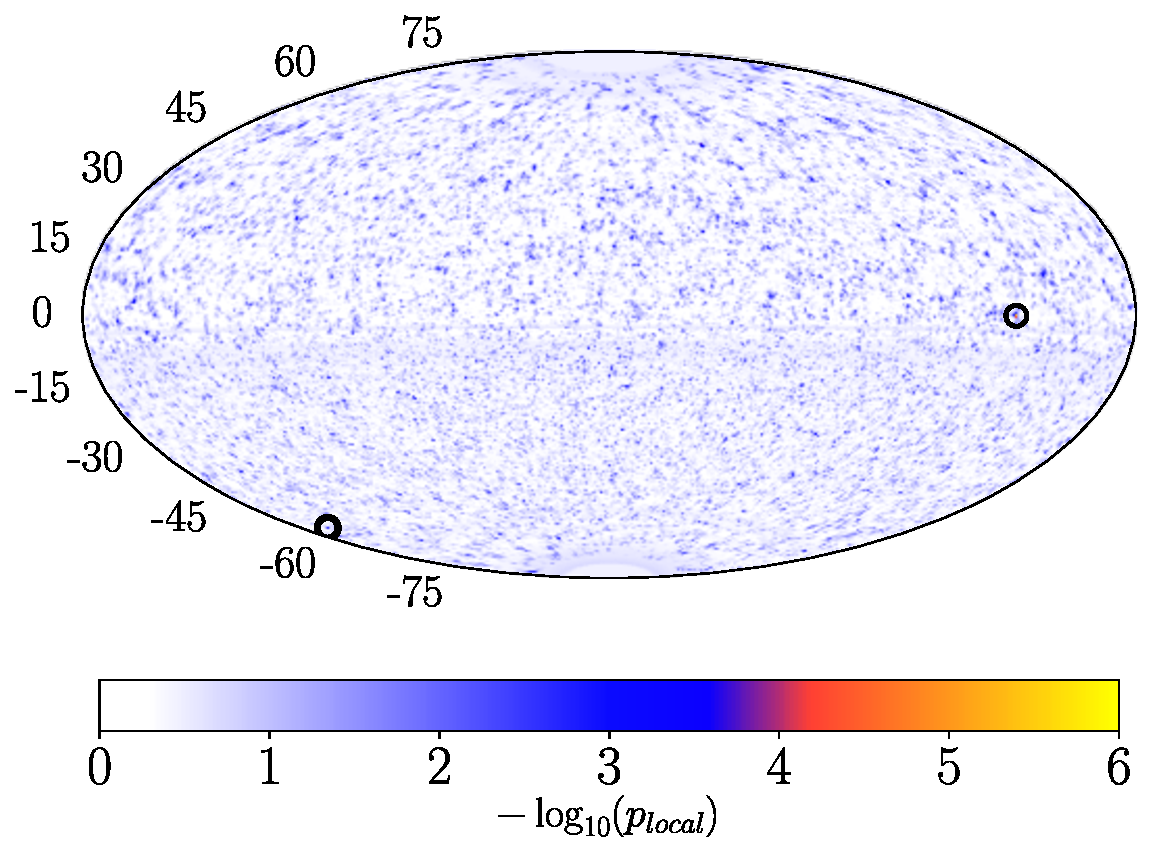
\includegraphics[width=0.6\linewidth]{img/IceCube_10yr_source_hotspot.pdf}
    \caption{IceCube对10年径迹型事件分析得到的中微子源的热点图。上下两个黑圈分别表示北天和南天最显著的源,分别是NGC 1068和PKS 2233-148。图片来自\cite{IceCube_10yr_point_source:2019}}
    \label{fig:IceCube_10yr_source_hotspot}
\end{figure}

通过对全天搜索得到的中微子源热点进行进一步的分析,IceCube发现了NGC 1068可能是一个中微子源\cite{IceCube_NGC1068:2022}。NGC 1068是一个距离地球仅为$14\,\mathrm{Mpc}$的Seyfert II型星系,它的中心有一颗被尘埃掩盖的超大质量黑洞\cite{Rosas_NGC_1068:2021}并且还是一个星爆星系。IceCube通过对径迹型事件进行分析,以$4.2\sigma$的置信度确认了NGC 1068是一个中微子源,其最佳拟合的中微子流量能谱如下:
\begin{equation}
\begin{aligned}
    \phi^{\nu_\mu+\bar{\nu}_\mu}(E_\nu) &= 
    \phi^{\nu_\mu+\bar{\nu}_\mu}_\mathrm{1\,TeV} 
    \times \left( \frac{E_\nu}{1\,\mathrm{TeV}} \right)^{-\gamma} 
    \times 10^{-11} \, \mathrm{s^{-1} cm^{-2} TeV^{-1}}, \\
    \phi^{\nu_\mu+\bar{\nu}_\mu}_\mathrm{1\,TeV} &= 
    5.0 \pm 1.5_\mathrm{stat} \pm 0.6_\mathrm{sys}, ~~
    \gamma = 3.2 \pm 0.2
    \label{eq:spectrum_NGC1068}
\end{aligned}
\end{equation}

对于实时暂现源的研究,IceCube设计了一套实时的多信使预警系统\cite{IceCube_alert:2016, IceCube_alert:2019},可以快速发布它观测到的高质量的中微子信号。
对于其他设备的观测结果,例如伽马射线和引力波等,IceCube中也存在一套跟随观测系统\cite{IceCube_follow_up:2020}用于快速发布可能的关联中微子信号或者给出中微子流量的上限。

2017年,IceCube观测到了一个约$270\,\mathrm{TeV}$的高能径迹型中微子事件(IceCube-170922A),该中微子事件与一个Fermi的耀变体数据库中的一个正在活跃期的耀变体TXS 0506+056在时间和空间上成协\cite{TXS_0506_MM:2018}。
而且通过对该方向上的中微子流量进行历史上的追溯搜索,IceCube发现该耀变体在2015年期间还有一次大规模的中微子流量超出,其置信度达到了$3.5\sigma$\cite{TXS_0506_flare:2018}。
这是人们首次成功地通过高能中微子事件来进行多信使观测,它打开了高能中微子多信使研究的大门。

除了对全天弥散的中微子流量进行点源搜寻以及通过实时多信使事件来搜寻暂现源,IceCube还对各种不同类别的中微子源进行了系统性的分类搜寻,其搜寻的分析和结果如下:

\begin{enumerate}
    \item \textbf{伽马射线暴}。IceCube对Fermi库中的GRB进行了时空上的成协分析,表明来自Fermi库中的GRB所产生的中微子辐射最多只能占弥散中微子流的$\sim 1\%$\cite{IceCube_GRB_prompt:2014, IceCube_GRB:2022}。尽管如此,来自低光度GRB和喷流被束缚的GRB(choked jet GRB)\cite{Choked_GRB:2015}对中微子流量的贡献依然无法被限制。

    \item \textbf{活动星系核和耀变体}。Fermi-2LAC的耀变体(blazar)样本与中微子的成协分析表明,这些耀变体最多贡献弥散中微子流的27\%。\cite{IceCube_Fermi_2LAC_blazars:2016}。另一项工作采用了不同的AGN样本,他们通过对软X射线辐射较强的AGN来进行相关性分析,然后也没有得到很高的置信度($2.6\sigma$)\cite{IceCube_AGN_core:2021}。

    \item \textbf{河内中微子源}。对于来自银河系内的中微子辐射,IceCube的分析表明其对弥散中微子流的贡献小于14\%\cite{IceCube_galactic:2017}。IceCube和ANTARES对银盘中微子流的联合分析没有找到明显的超出\cite{ANTARES_IceCube_galactic:2018}。IceCube对PWN和X射线双星的分析中都没有找到成协的源\cite{IceCube_PWN:2020, IceCube_X_binaries:2022}。IceCube中微子与HAWC\cite{IceCube_HAWC:2019}和LHAASO\cite{Huang_IceCube_LHAASO:2021, IceCube_LHAASO:2022}的高能伽马射线源的联合分析也没有找到中微子信号的超出。

    \item \textbf{快速射电暴}。IceCube对快速射电暴(Fast Radio Burst,FRB)样本进行过多次的时间和空间相关联的中微子信号寻找\cite{IceCube_FRB:2017, IceCube_FRB:2019, IceCube_FRB:2022},但都没有找到相关联的信号。

    \item \textbf{双致密星并合}。IceCube对LIGO-Virgo探测到的双致密星并合事件做过一些关联性分析\cite{GW170817_MM, IceCube_ANTARES_Auger_GW170817, IceCube_BBH:2020},分析中并没有找到中微子信号超出。

    \item \textbf{潮汐瓦解事件}。目前光学望远镜已经发现了3个与IceCube中微子信号在时间和空间上成协的的TDE事件\cite{TDE_MM:2023}:AT2019dsg\cite{AT2019dsg:2020},AT2019fdr\cite{AT2019fdr:2021}和AT2019aalc,而IceCube合作组尚未发表有关TDE和中微子信号的分析文章。

\end{enumerate}


\subsubsection{味道分辨}

来自天体物理源的高能中微子的味道测量对于研究中微子源内发生的物理过程以及寻找新物理有重要的意义\cite{Arguelles_flavor:2015, snowmass_flavor:2022}。根据标准模型的预言,在源处发射的味道为$\alpha$的中微子在经过超长基线振荡后转变为$\beta$味道的中微子的几率为\cite{Farzan_coherence_oscillation:2008}:
\begin{equation}
    \left\langle P_{\nu_\alpha \rightarrow v_\beta}\right\rangle=\sum_i\left|U_{\alpha i}\right|^2\left|U_{\beta i}\right|^2, 
    \label{eq:flavor_transform}
\end{equation}
其中$U$为公式\ref{eq: neutrino oscillation}中介绍的PMNS矩阵。

在假设中微子源处的味道比例为$\nu_e: \nu_\mu: \nu_\tau=1 / 3: 2 / 3: 0$,那么在地球中观测到的中微子的味道比例就应该是$\nu_e: \nu_\mu: \nu_\tau = 0.30 : 0.36 : 0.34$,与$1/3 : 1/3 : 1/3$相接近。
而在假设一些超出标准模型的效应,例如惰性中微子\cite{IceCube_sterile:2016, Arguelles_flavor_sterile:2019},洛伦兹对称性破缺\cite{IceCube_flavor_Lorentz:2017}等的情况下,地球上观测到的中微子味道的比例可能会与$1/3 : 1/3 : 1/3$发生强烈的偏离。

长期以来,IceCube都在从观测到的高能中微子数据中中微子味道比例\cite{IceCube_flux_flavor:2015, IceCube_inelestic_flavor:2018, IceCube_tau:2020}。
图\ref{fig:IceCube_flavor_ratio_measurement}展示了IceCube最新的测量结果。

\begin{figure}[htbp]
    \centering
    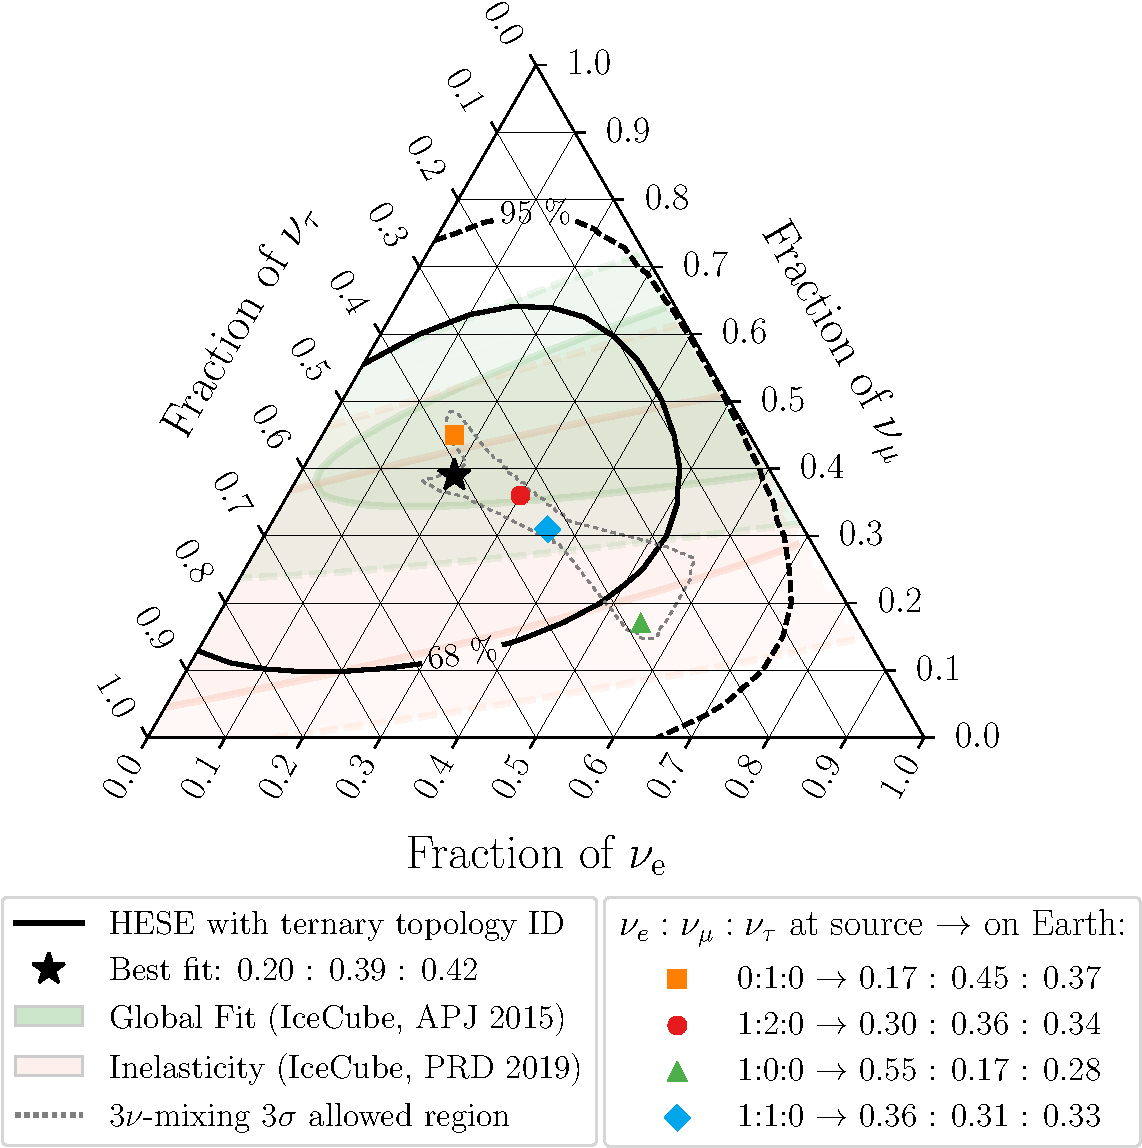
\includegraphics[width=0.9\linewidth]{img/IceCube_flavor_ratio_measurement.pdf}
    \caption{IceCube对中微子味道的测量结果以及理论预测值。途中的黑线\cite{IceCube_tau:2020},绿色阴影区域\cite{IceCube_flux_flavor:2015},粉色区域\cite{IceCube_inelestic_flavor:2018}分别表示IceCube三次用不同的方法实现的中微子味道的测量结果。实心的正方形,圆形,三角形,棱形分别表示几种典型的源处中微子味道比例所对应的地球上理论预期的比例。图片来自\cite{IceCube_tau:2020}}
    \label{fig:IceCube_flavor_ratio_measurement}
\end{figure}

    \chapter{大型切伦科夫中微子望远镜}
\label{ch:neutrino_telescope}

来自宇宙中的中微子的流量比较微弱,Waxman和Bahcall假设产生高能宇宙线的源对于$\pi$介子产生过程并非是不透明的,即并没有隐藏的超高能宇宙线源。由此他们根据观测到的超高能宇宙线的流量,利用章节\ref{subsubsec:neutrino_production}中所讨论的宇宙线产生中微子的方式,推导得到了著名的Waxman-Bahcall上限\cite{Waxman_Bahcall_bound:1999, Waxman_Bahcall_bound:2001}:
\begin{equation}
    E_\nu^2 \Phi_\nu < E_\nu^2 \Phi_\nu^{\mathrm{WB}} = 5 \times 10^{-8} \mathrm{GeV} \mathrm{cm}^{-2} \mathrm{~s}^{-1} \mathrm{sr}^{-1} ,
    \label{eq:Waxman_Bahcall_bound}
\end{equation}
其中$E_\nu$表示高能中微子的流量,$\Phi_\nu$表示中微子的流量,$\Phi_\nu^{\mathrm{WB}}$表示满足假设的情况下最大的中微子流量。
考虑到中微子与物质的作用几率非常的小,因此他们推断只有当靶物质的质量达到$10^{12}\,\mathrm{kg}$,$\mathrm{km}^3$量级,即体积达到$\mathrm{km}^3$量级之后,才有可能在年的时间制度内探测到宇宙中的高能中微子信号。

通过建造大体积的切伦科夫光中微子望远镜来探测高能天体中微子的想法早在1950年代便已经被提出了\cite{Telescope_history:2019}。
1960 年,M. Markov 发表了他的突破性想法 \cite{Markov:1960},即在湖泊或海洋等大型天然水体的深处安装光敏探测器阵列,从而实现对超大体积的介质进行监控。
这种望远镜借助了天然的介质来作为中微子反应的靶物质,是在人类在目前生产力水平下实现体积达到$10^{12}\,\mathrm{kg}$,$\mathrm{km}^3$级别的靶物质质量的有效途径。
而且它利用了粒子产生的切伦科夫光信号,这是因为介质中切伦科夫光信号的衰减距离($30-100\,\mathrm{m}$)要远远长于除缪子以外的大多数带电粒子($1,\mathrm{cm}-1\,\mathrm{m}$),从而可以扩大单个探测器的有效探测体积。
因此,望远镜中的光敏探测阵列可以布置得比较稀疏($~\mathcal{O}(100)\,\mathrm{m}$),从而实现以比较低廉的成本来监控如此庞大体积的反应介质。

值得一提的是,除了利用切伦科夫光来探测中微子以外,还有多种其他探测高能中微子的方式。例如我们可以利用射电信号来探测中微子,即借助于带电粒子簇射演化过程中的Askaryan效应\cite{askaryan_excess:1962}。
目前有不少项目在通过这种原理进行中微子探测,例如在中国建设的GRAND\cite{GRAND:2018},在格陵兰岛的冰层中探测的RNO-G\cite{RNO-G:2020},IceCube-Gen2中的射电阵列\cite{IceCube-Gen2_white_paper:2020}等等。
此外还可以利用声学信号的方式探测中微子\cite{Askarian_acoustic:1979},目前在Antares和KM3NeT的阵列中有所测试\cite{Lahmann_history_acoustic:2019, ANTARES_acoustic:2010, KM3NeT_acoustic:2022}。
相比于切伦科夫光,射电和声学信号都可以在海水中传播更远的范围,因此以这两种信号为媒介设计的中微子望远镜可以用更加稀疏的探测器阵列来覆盖相同的靶物质体积, 从而能够将可探测的能区延伸到事例率更少的超高能(EeV)能区。
但它们的缺点是信号噪声比较高,对中微子事件的重建精度相对较差。
本文主要讨论切伦科夫中微子望远镜,因此如不做特殊说明,在本文中的中微子望远镜均代指切伦科夫中微子望远镜


\section{探测机制}

\subsection{深度非弹性散射}

高能中微子在穿过介质的过程中,可以通过弱相互作用和介质中的原子核发生深度非弹性散射(deep-inelastic scattering,DIS)\cite{Sarkar_DIS:2011, Bertone_DIS:2019}过程并产生多种次级粒子,如图\ref{fig:DIS_types}中所示,这是将高能中微子转换为易被观测的电磁粒子的主要反应通道:
\begin{equation}
    \begin{aligned}
        & \nu_l + N \rightarrow \nu_l + X \\
        & \nu_l + N \rightarrow l + X ,
    \end{aligned}
\end{equation}
其中$\nu_l$表示高能中微子,$N$表示靶原子核,$l$表示产生的轻子,$X$表示原子核碎裂后经过强子化过程产生的强子簇射。

DIS过程的反应截面与原子核的部分子分布函数(parton distribution function, PDF)有关。PDF是在描述原子核内部找到某一能量的部分子(夸克或者胶子)的概率,是计算强相互作用所必须的\cite{Soper_PDF:1997, NNPDF_PDF:2017}。

下面,我们以带电流反应为例,介绍中微子与原子核之间的DIS作用,它的反应截面可以用以下的结构函数来表示:
\begin{equation}
\begin{aligned}
    \frac{\mathrm{d}^2 \sigma_{\nu(\bar{\nu}) N}^{\mathrm{CC}}\left(x, Q^2, E_\nu\right)}{\mathrm{d} x \mathrm{~d} Q^2}= & \frac{G_F^2 M_W^4}{4 \pi x\left(Q^2+M_W^2\right)^2} \\
    & \times\left(Y_{+} F_{2, \mathrm{CC}}^{\nu(\bar{\nu}) N}\left(x, Q^2\right) \mp Y_{-} x F_{3, \mathrm{CC}}^{\nu(\bar{\nu}) N}\left(x, Q^2\right)-y^2 F_{L, \mathrm{CC}}^{\nu(\bar{\nu}) N}\left(x, Q^2\right)\right) ,
\end{aligned}
\end{equation}
其中$xF_3$项前面的正号对应中微子,负号对应反中微子。$Y_\pm = 1 \pm (1-y)^2$,$y$是Bjorken参数,也称为非弹性系数,是DIS过程中Bjorken尺度效应的参数之一:
\begin{equation}
\begin{aligned}
    Q^2 & =-q^2, \quad y=\frac{q \cdot p}{k \cdot p}=1-\frac{E^{\prime}}{E_\nu}, \quad x=\frac{Q^2}{2 q \cdot p}=\frac{Q^2}{2 m_N y E_\nu} \\
    W^2 & =(p+q)^2=m_N^2+Q^2\left(\frac{1}{x}-1\right), \quad s=(k+p)^2=m_N^2+2 E_\nu m_N,
\end{aligned}
\end{equation}
其中$k$,$q$和$p$分别是在打靶实验室系下的中微子,规范玻色子和原子核的四动量。$E^{\prime}$和$E_\nu$分别表示出射的轻子和入射的中微子的能量。

\begin{figure}[htb]
    \centering
    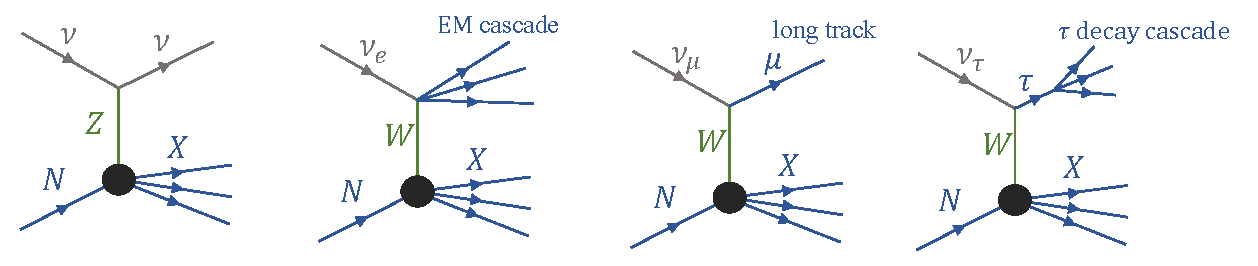
\includegraphics[width=0.95\linewidth]{img/DIS_types.pdf}
    \caption{中微子与原子核发生DIS过程的示意图}
    \label{fig:DIS_types}
\end{figure}

中微子与质子的DIS过程的总反应截面如图\ref{fig:DIS_cross_section}所示。对于中微子望远镜的研究而言,DIS的散射截面决定了其能够探测到的事件率,而反过来中微子可以通过不同入射角的中微子穿透地球的概率来估计中微子的散射截面\cite{IceCube_cross_section:2020}。对于中微子望远镜的研究来说,以下DIS散射截面的特点是比较重要的:
\begin{enumerate}
    \item 在能量比较高处($E_\nu \gtrsim 1 \,\mathrm{TeV}$),中微子和反中微子的散射截面几乎相同,而带电流的散射截面大约是中性流的两倍。
    \item 在极高能处($E_\nu \gtrsim 1 \,\mathrm{PeV}$),散射截面有如下关系$\sigma_{\nu(\bar{\nu})N} \propto E_\nu^{0.36}$。
    \item $\mathrm{Bjorken}-y$参数的平均值会随着中微子能量的增加而逐渐减小,如图\ref{fig:Bjorken_y}所示。
    \item 平均自由程大约等效于地球直径的中微子的能量大约为$40\,\mathrm{TeV}$。
\end{enumerate}

\begin{figure}[htb]
    \centering
    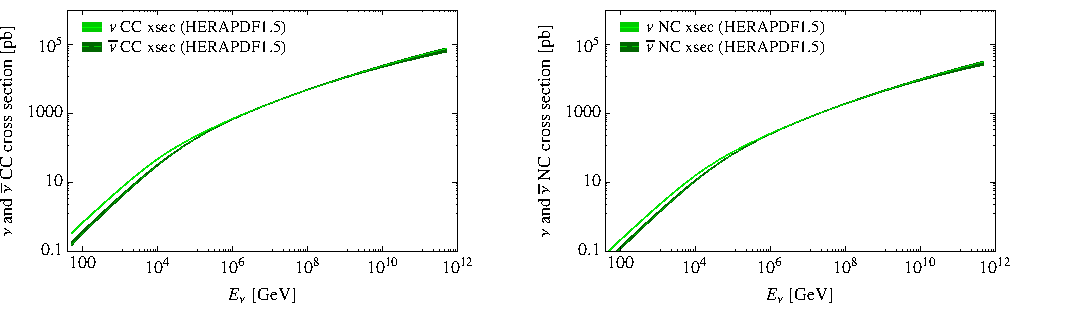
\includegraphics[width=0.95\linewidth]{img/DIS_cross_section.pdf}
    \caption{中微子与同位旋为0的原子核发生DIS过程的散射截面。左图:带电流反应;右图:中性流反应。图片来自\cite{Sarkar_DIS:2011}}
    \label{fig:DIS_cross_section}
\end{figure}

\begin{figure}[htb]
    \centering
    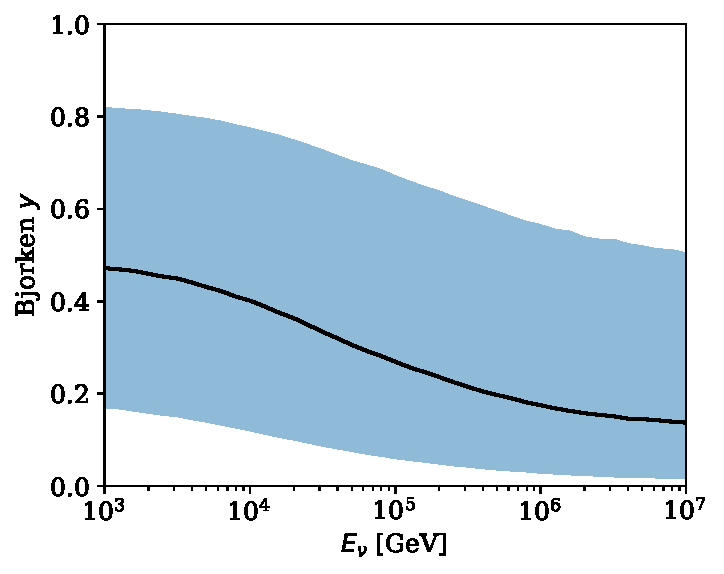
\includegraphics[width=0.7\linewidth]{img/Bjorken_y.pdf}
    \caption{$\mathrm{Bjorken}-y$与中微子能量的关系。黑线表示中位数,蓝色阴影带表示$1\sigma$范围。数据由Pythia-8.3\cite{Pythia8.2:2014, Pythia8.3:2022}模拟得到。}
    \label{fig:Bjorken_y}
\end{figure}

在能量比较低的区域,除了DIS过程外,中微子和物质的反应还包括准弹性散射(quasielastic scattering)和共振散射(resonance  production)。
在前者中,中微子可以从原子核中撞出一部分核子,而在后者中,原子被中微子激发到激发态(如$\Delta$,$N^*$)再快速衰变\cite{CS_Formaggio:2012}。
在低能处,中微子通过带电流的不同反应通道的散射截面如图\ref{fig:DIS_cross_section_le}所示。

\begin{figure}[htb]
    \centering
    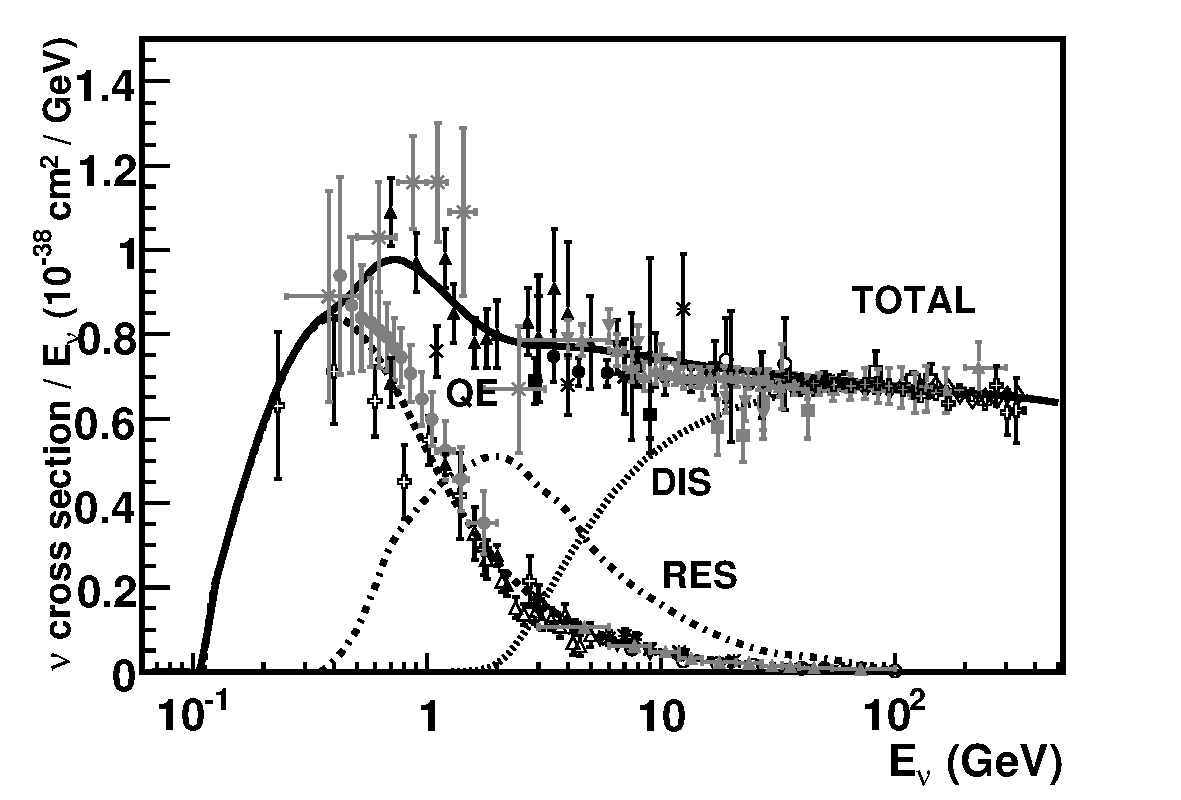
\includegraphics[width=0.45\linewidth]{img/cross_section_le_CC.pdf}
    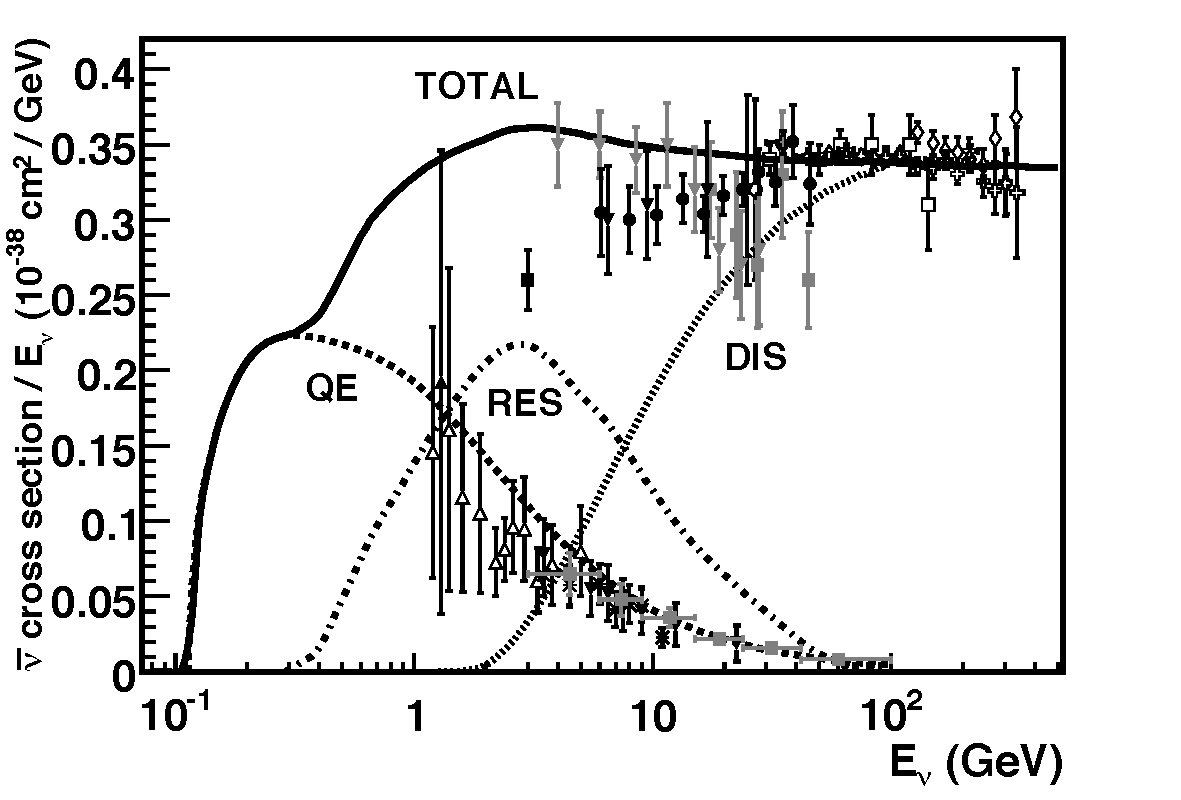
\includegraphics[width=0.45\linewidth]{img/cross_section_le_CCbar.pdf}
    \caption{低能处,中微子与原子核通过带电流的发生各种不同通道的散射截面。左图:正中微子,右图:反中微子。图片来自\cite{CS_Formaggio:2012}}
    \label{fig:DIS_cross_section_le}
\end{figure}




\subsection{切伦科夫辐射}

\begin{figure}[htb]
    \centering
    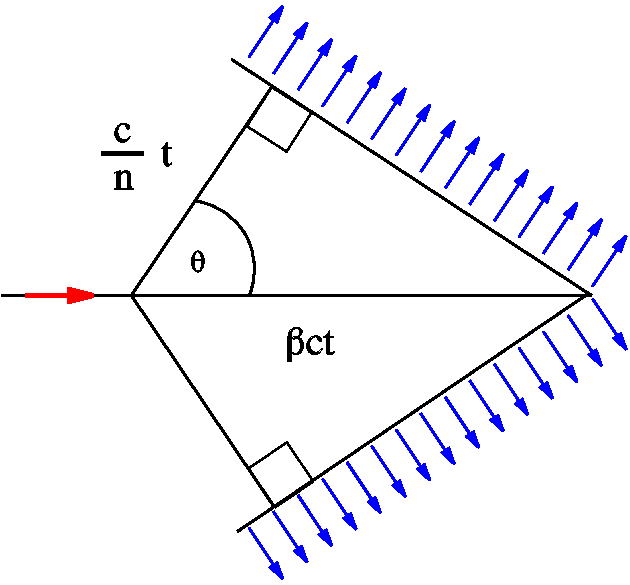
\includegraphics[width=0.4\linewidth]{img/Cherenkov_geometry.pdf}
    \caption{切伦科夫辐射的几何示意图。}
    \label{fig:Cherenkov_geometry}
\end{figure}

当带电粒子在介质中的运动速度超过介质中的光速时,便可以产生切伦科夫辐射,那是一种可以传播到远处的相干电磁辐射。
如图\ref{fig:Cherenkov_geometry}所示,切伦科夫光具有很强的方向性。切伦科夫光子与产生它的带电粒子的运动方向的夹角,即切伦科夫角$\theta_C$,满足如下关系:
\begin{equation}
    \cos \theta_\mathrm{CK}=\frac{1}{\beta n_\mathrm{p}} , 
\end{equation}
其中$\beta = v / c$是带电粒子的运动速度和光速之间的比值,$n_\mathrm{p}$表示介质的折射率。

切伦科夫光的辐射能谱可以用Frank–Tamm公式来表示:
\begin{equation}
    \frac{\mathrm{d}^2 N_\mathrm{ph}}{\mathrm{d}E_\mathrm{ph} \mathrm{d}x} = 
    \frac{2 \pi \alpha}{hc}\left(1 - \frac{1}{\beta^2 n_\mathrm{p}^2(\lambda)} \right) = 
    \frac{2 \pi \alpha}{h c} \sin^2\theta_C \simeq 
    370 \sin^2\theta_C ~\mathrm{\frac{photons}{cm \cdot eV}}
    \label{eq:Frank–Tamm}
\end{equation}
其中$\frac{\mathrm{d}^2 N_\mathrm{ph}}{\mathrm{d}E_\mathrm{ph} \mathrm{d}x}$表示在单位距离$x$中,辐射出单位能量$E_\mathrm{ph}$的光子数目$N_\mathrm{ph}$,$h$是普朗克常数。

将物理常数代入到Frank–Tamm公式并考虑到海水的折射率约为1.35以及可见光的可观测能量带约为$1\,\mathrm{eV}$(对应$350\,\mathrm{nm}$到$600\,\mathrm{nm}$的波长范围),可以得到一条简易的经验公式:一个接近光速运动的带电粒子可以在每厘米的径迹长度上产生约400个切伦科夫光子。再考虑带点粒子簇射的主要能量沉积方式为电子电离能损,而电子电离能损的强度约为$2.2\,\mathrm{MeV/cm}$。由此,我们可以得到经验公式:
\begin{equation}
    \frac{\mathrm{d} N_\mathrm{ph}}{\mathrm{d} E_\mathrm{dep}} = 
    \frac{\mathrm{d} N_\mathrm{ph}}{\mathrm{d}x} / \frac{\mathrm{d} E_\mathrm{dep}}{\mathrm{d}x} \simeq
    200 \frac{\mathrm{photons}}{\mathrm{MeV}}
    \label{eq:emission_efficiency}
\end{equation}
其中$E_\mathrm{dep}$表示高能粒子簇射在介质中沉积的能量。从这个经验关系中,我们可以得知即高能的带电粒子在海水介质中以切伦科夫光的形式辐射的光产额为$\sim 200 \mathrm{MeV}^{-1}$。

\subsection{数字光学模块}

中微子望远镜依赖于在透明介质中布置的数字光学模块(digital optical module, DOM)来探测中微子反应产生的带电次级粒子所引发的切伦科夫光信号。
以IceCube为例,它包含86根挂满DOM的根垂直探测单元(string,以下简称为串列单元),每个串列单元上挂载有60个DOM\cite{IceCube_detector:2016}。
IceCube中的DOM阵列的水平间距约为$125\,\mathrm{m}$,垂直间距为$17\,\mathrm{m}$,该阵列可以监控$1\,\mathrm{km}^3$体积的冰体。

IceCube中的使用的DOM外部是一个外直径13英寸,厚度0.5英寸的抗压玻璃球,用于保护内部的电子学设备。抗压玻璃球可以长期抵抗$250\,\mathrm{bar}$(等效于$2.6\,\mathrm{km}$的水深)的压强。
玻璃球壳要求在可见光和近紫外波段拥有高透射率,这是为了降低对本身就微弱的切伦科夫光信号的损耗。此外玻璃球壳还要求有较低的放射性背景,从而减少额外的噪声。

IceCube的DOM中包含一支日本滨松公司生产的10英寸的光电倍增管(photonmultiplier tube,PMT)\cite{IceCube_PMT:2010}。
PMT的原理如图\ref{fig:PMT_structure}所示,它借助光电效应将入射到PMT的光阴极的光子转换为光电子,并利用高压在PMT的倍增极(也称打拿级)之间产生强大的电厂,从而将电子提高电子的动能,使其在撞击下一个倍增级时能激发出更多的光子。通过多级放大,PMT可以将电子信号放大到$\mathcal{O}(10^6)$倍,这些电子最终会汇聚到阳极,产生宏观上可被观测和数字化的电流。

\begin{figure}[htb]
    \centering
    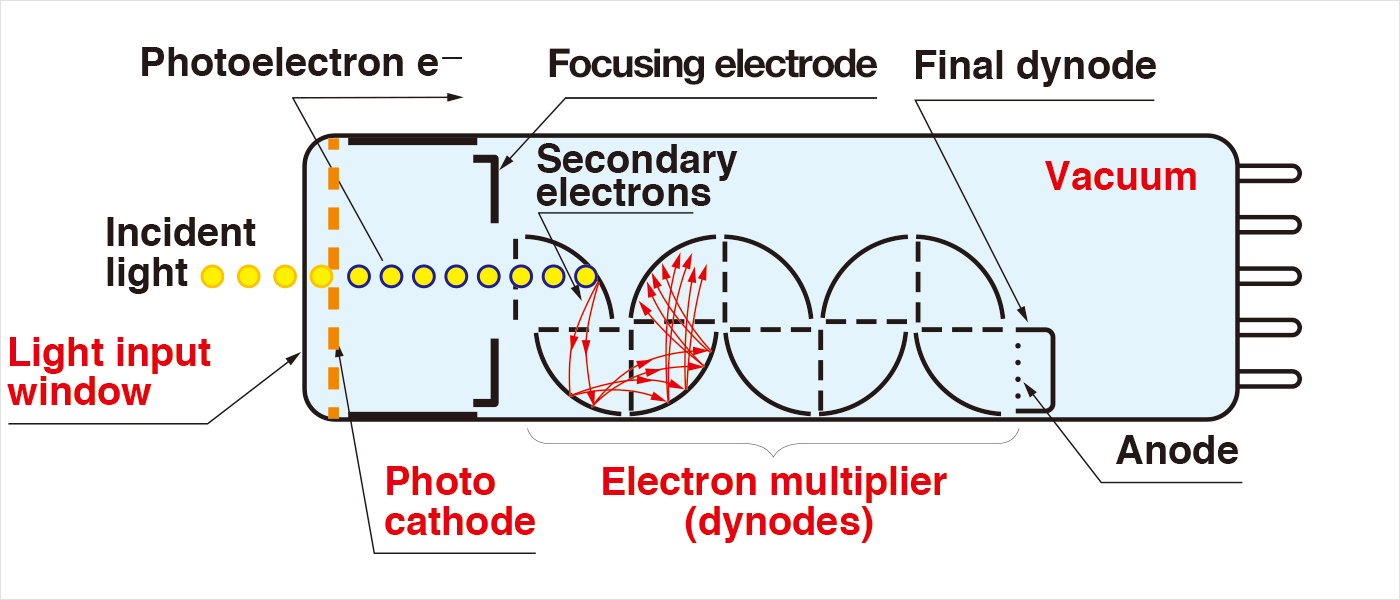
\includegraphics[width=0.85\linewidth]{img/PMT_structure.png}
    \caption{PMT的结构和工作原理示意图。图片来自\cite{PMT_handbook:2016}}
    \label{fig:PMT_structure}
\end{figure}

PMT是非常灵敏的单光子探测设备,是中微子望远镜用来观测中微子信号的眼睛。在我们的应用中,对PMT感兴趣的主要性能参数有:

\begin{enumerate}
    \item 量子效率(quantum efficiency)。表示入射到光阴极的光子能够产生有效的光电子的概率。
    \item 增益(gain)。表示光电子在经过了多个倍增级放大之后,最终在阳极处的电子数量,即电子数量的放大率。
    \item 单光子波形(single photoelectron waveform)。表示单个光子产生的电压波形信号的形状。通常用波形的高度,上升时间和下降时间等量来表征。
    \item 单光子分辨率(single photoelectron resolution)。用于表示PMT分辨单光子信号和零光子背景噪声的能力,通常用光电子电荷量分布图中的单光子峰与零光子峰之间的峰谷比来表征。
    \item 渡越时间弥散(transient time spread)。渡越时间表示由电子在经过多个倍增极后最终到达阳极形成电流所需要的时间。而渡越时间弥散便表示电子在放大和穿行的这段时间的不确定度,它最终会体现在PMT产生的电压波形信号的上升沿时间点的弥散。
\end{enumerate}

为了避免玻璃球-空气-PMT之间由于折射率不同所带来的界面效应而引发的光子损耗,IceCube在玻璃球壳和PMT中间填充了光学胶。光学胶需要在我们的探测光的波段范围内具有高透光性($>90\%$),并且拥有$\gtrsim 1.4$的折射率,接近于玻璃的$\sim 1.5$折射率。
对于IceCube这种装备单个大英寸的PMT的DOM而言,其PMT中电子倍增放大的过程会受到地球磁场的影响,因此还需要在PMT外围包裹一层金属网罩来屏蔽地球磁场的影响\cite{pmt_Earth_magnetic:2011}。

在通过PMT将光信号转换为电信号后,需要前端读数电路将光电子的模拟信号数字化。IceCube的读数电路具有波形读出的能力,即将连续的光电子电压波形采样成离散的数据点,如图\ref{fig:IC_waveform}所示\cite{IceCube_DAQ:2008}。
IceCube拥有两种不同时间精度的波形采样设备:精度较高的是两块ATWD(Analog Transient Waveform Digitizer)芯片,它们拥有$300\,\mathrm{MHz}$的采样频率和$10\,\mathrm{bit}$的采样精度,但只能连续采样128个数据点,即连续采样$428\,\mathrm{ns}$的波形数据;精度较低的是fADC(fast Analog Digital Converter)\footnote{尽管名字中带有fast,但是$40\,\mathrm{MHz}$的采样频率在2020年代已经相对比较慢了。},它拥有$40\,\mathrm{MHz}$的采样频率和$10\,\mathrm{bit}$的采样精度并且可以连续256个数据点,即采样时间可以达到$6.4\,\mathrm{\mu s}$,足以包含绝大多数的中微子事件以及其后脉冲。

IceCube中的ATWD不同于可以连续采样的ADC,是一种SCA(Switched Capacitor Arrays)。它通过先将电压信号储存在电容器阵列中,再利用相对低速的ADC从电容阵列中读取电压值的形式,从而在低功耗的情况下实现高时间精度的采样\cite{DRS4:2010}。
ATWD的应用帮助IceCube在2000年代便达到了$300\,\mathrm{MHz}$的信号采样频率,为分析中微子信号提供了有力的支撑。这些高精度的波形信号还可以被用于寻找陶中微子所对应的双峰波形结构,提高了IceCube对中微子味道的分辨能力\cite{IceCube_tau_Donglian:2015, IceCube_tau_Logan:2019, IceCube_tau:2020}。
SCA技术路线的弊端是需要等待低速ADC读取电压,因而会有比较长的死时间。以IceCube中的ATWD为例,死时间有$29\,\mu\mathrm{s}$,因此IceCube设计了双ATWD芯片的备用机制,用于应对时间上紧密相邻的信号。

在新一代的中微子望远镜中,人们开始尝试在数字光学模块中使用多个小型的PMT来代替单个大型的PMT。
例如KM3NeT中采用了一个mDOM(multi DOM)的探测模块,每一个玻璃球内都包含有31个具有独立采数通道的PMT,通过对要求同时有多个PMT接收到光子信号,可以有效避免PMT自身的暗噪声以及海水的光学噪声背景的影响\cite{KM3NeT_mDOM:2015}。
IceCube-Gen2中也计划使用包含多个PMT的mDOM\cite{IceCube-Gen2_mDOM:2021}。
这些有关新光学模块的技术将会在一个中间项目——IceCube-upgrade\cite{IceCube-upgrade:2019}中进行研究和测试\cite{IceCube_upgrade_mDOM:2021, IceCube_D-Egg:2022}。
我们团队也有进行新型数字光学模块的设计,我们提出了hDOM(hybrid DOM)\cite{hDOM:2021}的设计构想,即在一个模块中即加入PMT又加入SiPM,从而提高模块的时间分辨率和感光面积。hDOM的设计和优势将会在章节\ref{sec:hdom}中具体介绍。

除了对光敏元件进行改造外,新一代的中微子望远镜还会采用更加现代化的电子学设计。
近10年来的数字电路数字电路部分则发生了天翻地覆的变化,我们需要着重考虑采用这些新型的技术,例如小白兔时钟同步\cite{white_rabbit:2013},性能更好的高速ADC\cite{Changda_PandaX_ADC:2021},通过更加强大的FPGA芯片来实现复杂的后端采数和触发的算法等。

\begin{figure}[htb]
    \centering
    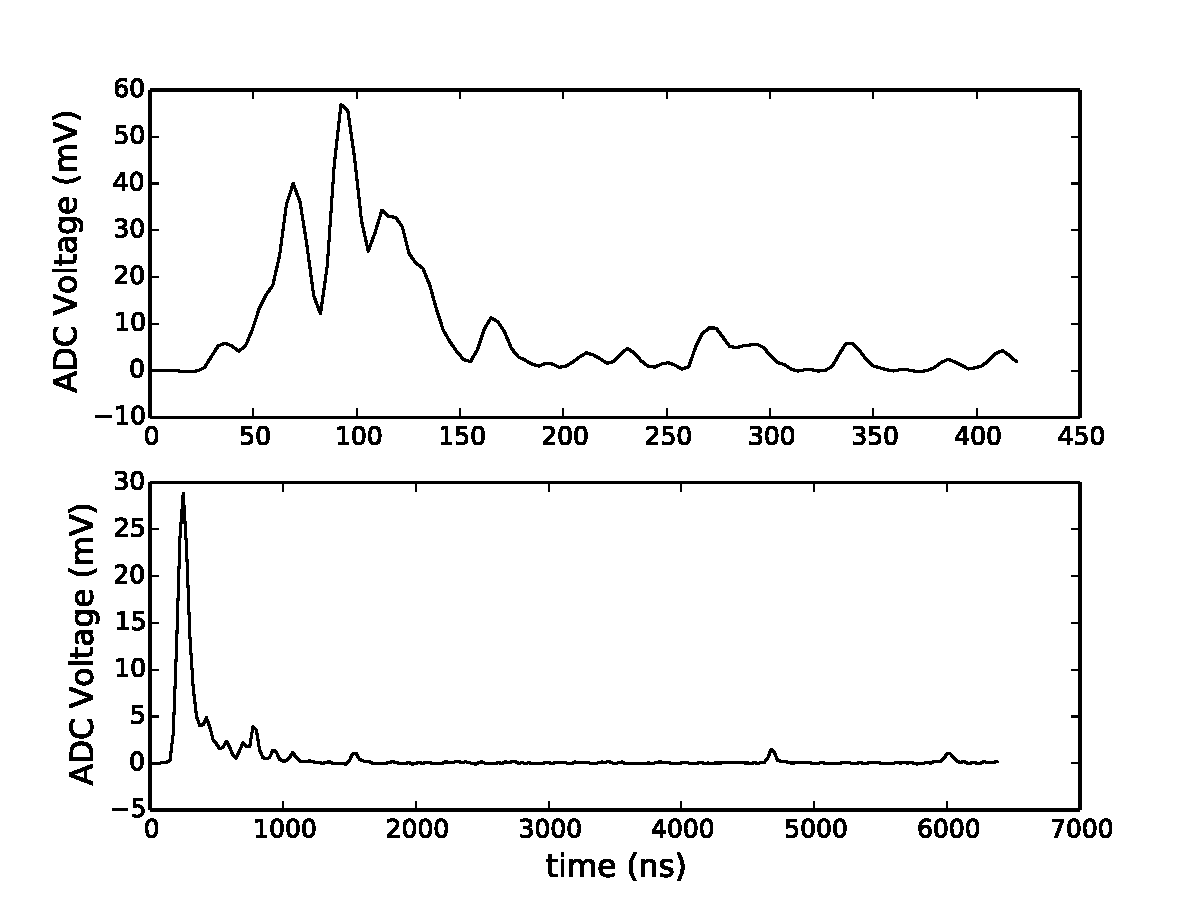
\includegraphics[width=0.8\linewidth]{img/IC_waveform.pdf}
    \caption{IceCube中对PMT产生的光电子电压信号采样得到的波形。图片来自\cite{IceCube_detector:2016}}
    \label{fig:IC_waveform}
\end{figure}

\begin{figure}[htb]
    \centering
    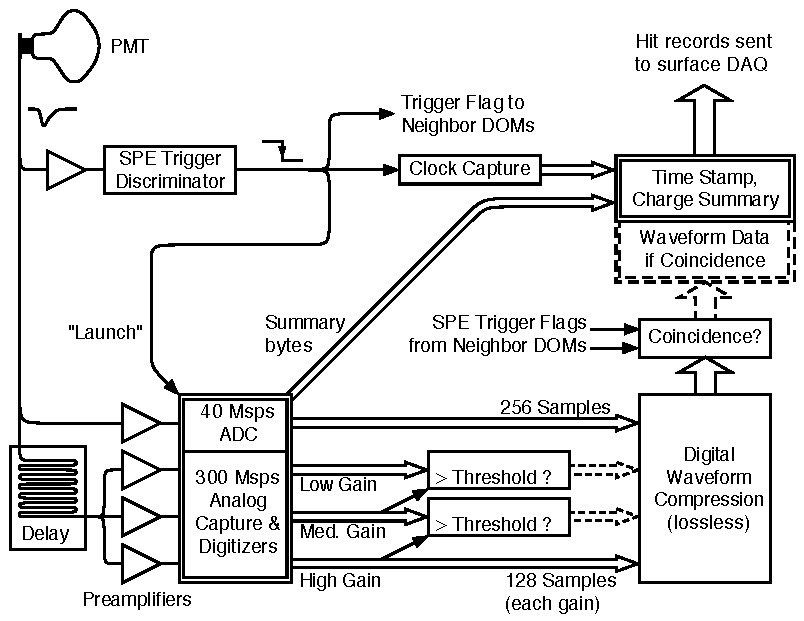
\includegraphics[width=0.8\linewidth]{img/IC_DOM_data_flow.pdf}
    \caption{IceCube中DOM对PMT采集到的信号进行数字化的流程图。图片来自\cite{IceCube_detector:2016}}
    \label{fig:IC_DOM_data_flow}
\end{figure}

\subsection{中微子事件类型}

如图\ref{fig:DIS_types}中所示,不同味道和不同反应通道的中微子发生DIS的产物不同,最终在DOM阵列中观测到的事件形态也有所不同,通常人们将中微子事件分为以下三种类型:
\begin{enumerate}
    \item 径迹型事件(track event):由缪子中微子通过带电流通道产生的缪子所产生的事件类型。
    \item 簇射型事件(cascade event):由电子中微子通过带电流流通道产生的的电子,或者所有味道的中微子通过中性流通道产生的强子簇射所产生的事件类型。
    \item 双簇射型事件(double-cascade event)由陶中微子通过带电流产生陶子的同时形成强子簇射,以及陶子衰变产生簇射,所组合而成的事件类型。
\end{enumerate}

\begin{figure}[htb]
    \centering
    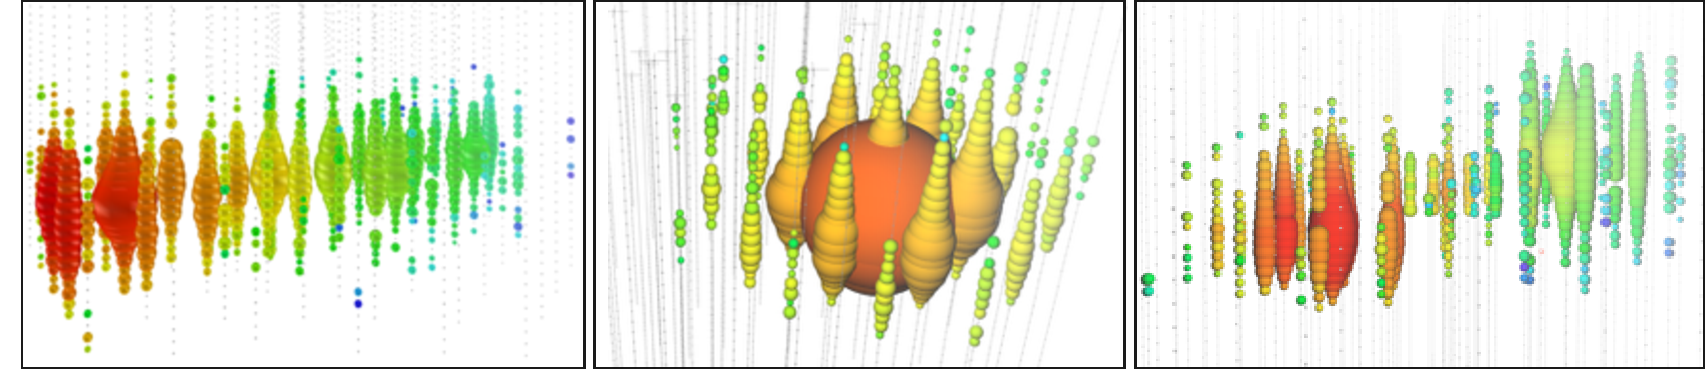
\includegraphics[width=1.0\linewidth]{img/event_topologies.pdf}
    \caption{IceCube模拟得到的DOM观测到的不同形态的中微子事件。左图对应径迹型事件,中图对应簇射型事件,右图对应双簇射型事件。图中每一个有颜色的点表示DOM观测到了来自中微子事件的光子,其颜色表示光子到达时间,大小表示DOM接收到的光子数量。图片来自\cite{IceCube-Gen2_white_paper:2020}}
    \label{fig:event_topologies}
\end{figure}


这些不同类型的中微子的形态特征如图\ref{fig:event_topologies}所示。由缪子中微子产生的缪子能够在介质中穿行数公里,形成鲜明的径迹型事件。这种事件通常可以重建得到最好的角度分辨能力\cite{AMANDA_track_reco:2003, IceCube_track_reco:2021, KM3NeT_reco:2017, Baikal_track_reco:2021},因而常被用于寻找中微子的天体物理起源\cite{IceCube_10yr_point_source:2019, KM3NeT_sensitivity:2018, ANTARES_IceCube_point_source:2020}。
但这种事件有比较高的背景,因为宇宙线轰击大气形成簇射的过程中也会产生缪子和中微子,在探测器阵列中产生径迹型事件。
在IceCube所处的深度,这些大气缪子的流量在$\mathrm{TeV}$能级处大约是天体物理起源中微子的流量的$\mathcal{O}(10^4)$倍\cite{IceCube_atmos_muon_flux:2018}。因此在数据分析时,人们通常选用来自地心那一侧或者能量比较高的径迹型事件,来减少大气缪子和大气中微子的干扰的影响。

另外一种有效去除大气缪子背景的方式是在径迹型事件和簇射型事件中进一步选取初始径迹型事件(starting-track event)\cite{IceCube_starting_track:2021}。
在这种事件中,缪子中微子与原子核DIS反应的顶点就发生在探测器内部,因而可以和来自大气中并且会经过探测器阵列外围的DOM的缪子背景进行区分。
同时这种方法可以通过屏蔽与大气缪子在时间上成协的信号来降低大气中微子的噪声\cite{IceCube_atmos_neutrino_flux:2016}。
但是由于在事件筛选和方向重建方面的困难以及事件样本数量的缺少,这种信号通道并没有得到大规模的应用\cite{IceCube_starting_track:2021b}。

簇射型事件通常拥有更好的能量分辨率\cite{IceCube_energy_reco:2013, KM3NeT_reco:2017, Baikal_cascade_reco:2022},可以用于很好地测量天体物理中微子的流强\cite{IceCube_6yr_cascade_spectrum:2020}。
在IceCube中,由于簇射型事件的角度重建精度比较差\cite{IceCube_cascade_dir_reco:2019, IceCube_cascade_dir_reco:2021},一般为10度左右,故较少用于做中微子的点源搜寻\cite{IceCube_cascade_source_search:2016}。
而在水基的望远镜中,例如KM3NeT和Baikal-GVD,由于深水的散射要远小于冰中的散射\cite{OP_ANTARES:2004, OP_Baikal:2012, OP_Grace:2018, OP_IceCube:2006, OP_NEMO:2006, OP_P-One:2021},故可以对簇射型事件进行较好的方向重建,其重建精度可以达到几度的水平\cite{KM3NeT_reco:2017, Baikal_cascade_reco:2022},在这种情况下,簇射型事件也可以被用于做多信使方面的研究\cite{Baikal_cascade_events:2019, Baikal_TXS:2022}。

双簇射型事件只能通过陶中微子的带电流作用产生,因此它可以用于寻找陶中微子\cite{IceCube_tau_Donglian:2015, IceCube_tau_Logan:2019, IceCube_tau:2020, Baikal_double_cascade_tau:2023, KM3NeT_double_cascade_tau:2021}。
双簇射型事件的第一个簇射是原子核被中微子DIS过程击碎后产生的强子簇射,第二个簇射是陶轻子衰变产生的电磁簇射($18\%$)或者强子簇射($\sim 65\%$)。而在剩余的衰变通道($17\%$)中,陶轻子衰变产生一个缪子,形成与初始径迹型事件类似的事件形态。

陶轻子的寿命$t_\mathrm{decay} = 3\times10^{-13}s$非常地短暂,但是在洛伦兹变化下,高能的陶轻子在实验室系下的时间流逝速度会变缓,因而可以飞行比较长的距离。陶轻子在衰变前的飞行距离$l_\tau$和陶轻子能量$E_\tau$由如下关系:
\begin{equation}
    l_\tau = \frac{E_\tau}{m_\tau} \times c t_\mathrm{decay} \simeq 50\,\mathrm{m} \times \frac{E_\tau}{1\,\mathrm{PeV}} ,
    \label{eq:tau_decay}
\end{equation}
其中$c$为光速,而$m_\tau=1.776 \,\mathrm{GeV}$为陶轻子的质量。考虑到探测器对簇射顶点的重建精度约为$3\,\mathrm{m}$,而且单个高能簇射在纵向上的尺度约为$10\,\mathrm{m}$,因此只有能量达到$\gtrsim 100 \, \mathrm{TeV}$的陶中微子事件才能产生容易分辨的双簇射型信号。

双簇射型事件除了可以从几何特征的上寻找外\cite{IceCube_tau:2020},还可以根据时间特征来寻找。
这两个簇射在到达DOM的时间上存在一定的先后关系,因而会在PMT的波形上形成双脉冲的结构,用时间方法寻找到的陶中微子事件也被称为双脉冲型事件\cite{IceCube_tau_Donglian:2015, IceCube_tau_Logan:2019, Tian_tau_double_pulse:2021}。
这两种测量方法分别对中微子望远镜阵列的空间和时间分辨能力有一定的要求。

\section{台址选择}

\subsection{介质的光学性质}

海水的光学性质,主要指海水的吸收长度和散射长度。光学性质决定了中微子望远镜所探测到的切伦科夫光信号的强度和质量,进而对望远镜探测的能量阈值,角分辨率等性能都有重要的影响,是在设计望远镜阵列的几何排布时要考虑的主要因素。
因此,几乎所有的望远镜都会对选址处的光学性质开展原位的测量和分析\cite{OP_ANTARES:2004, OP_Baikal:2012, OP_Grace:2018, OP_IceCube:2006, OP_IceCube:2013, OP_NEMO:2006, OP_P-One:2021}。

\subsection{纬度位置}

与光学和射电的望远镜类似,中微子望远镜也拥有一段最灵敏的探测区域,我们称之为灵敏带。
中微子望远镜对来自水平方向上的中微子流强拥有最好的灵敏度,这是因为在水平方向上的屏蔽层柱密度的大小适中,即能保证将大气缪子全部吸收,又不至于吸收高能的中微子事件。

中微子望远镜所处的纬度位置决定了它的灵敏带能够覆盖的天区范围,如图\ref{fig:detector_poistion_and_sensitive_band}中所示。
位于南极的IceCube的灵敏带在赤道坐标系下是一条水平的环带,由于IceCube坐落在南极点,因此它和它的灵敏带都不会随着地球的转动而发生转动。
位于其他区域的中微子望远镜的灵敏带会随着地球的自转扫过不同的天区,特别的,靠近赤道上的中微子望远镜的灵敏带能够扫过整个天区。
坐落在地球不同位置的中微子望远镜可以形成互补的大型高能中微子观测网络\cite{PLENuM:2021},其灵敏带能够覆盖全天各个方向的中微子源。


\begin{figure}[htb]
    \centering
    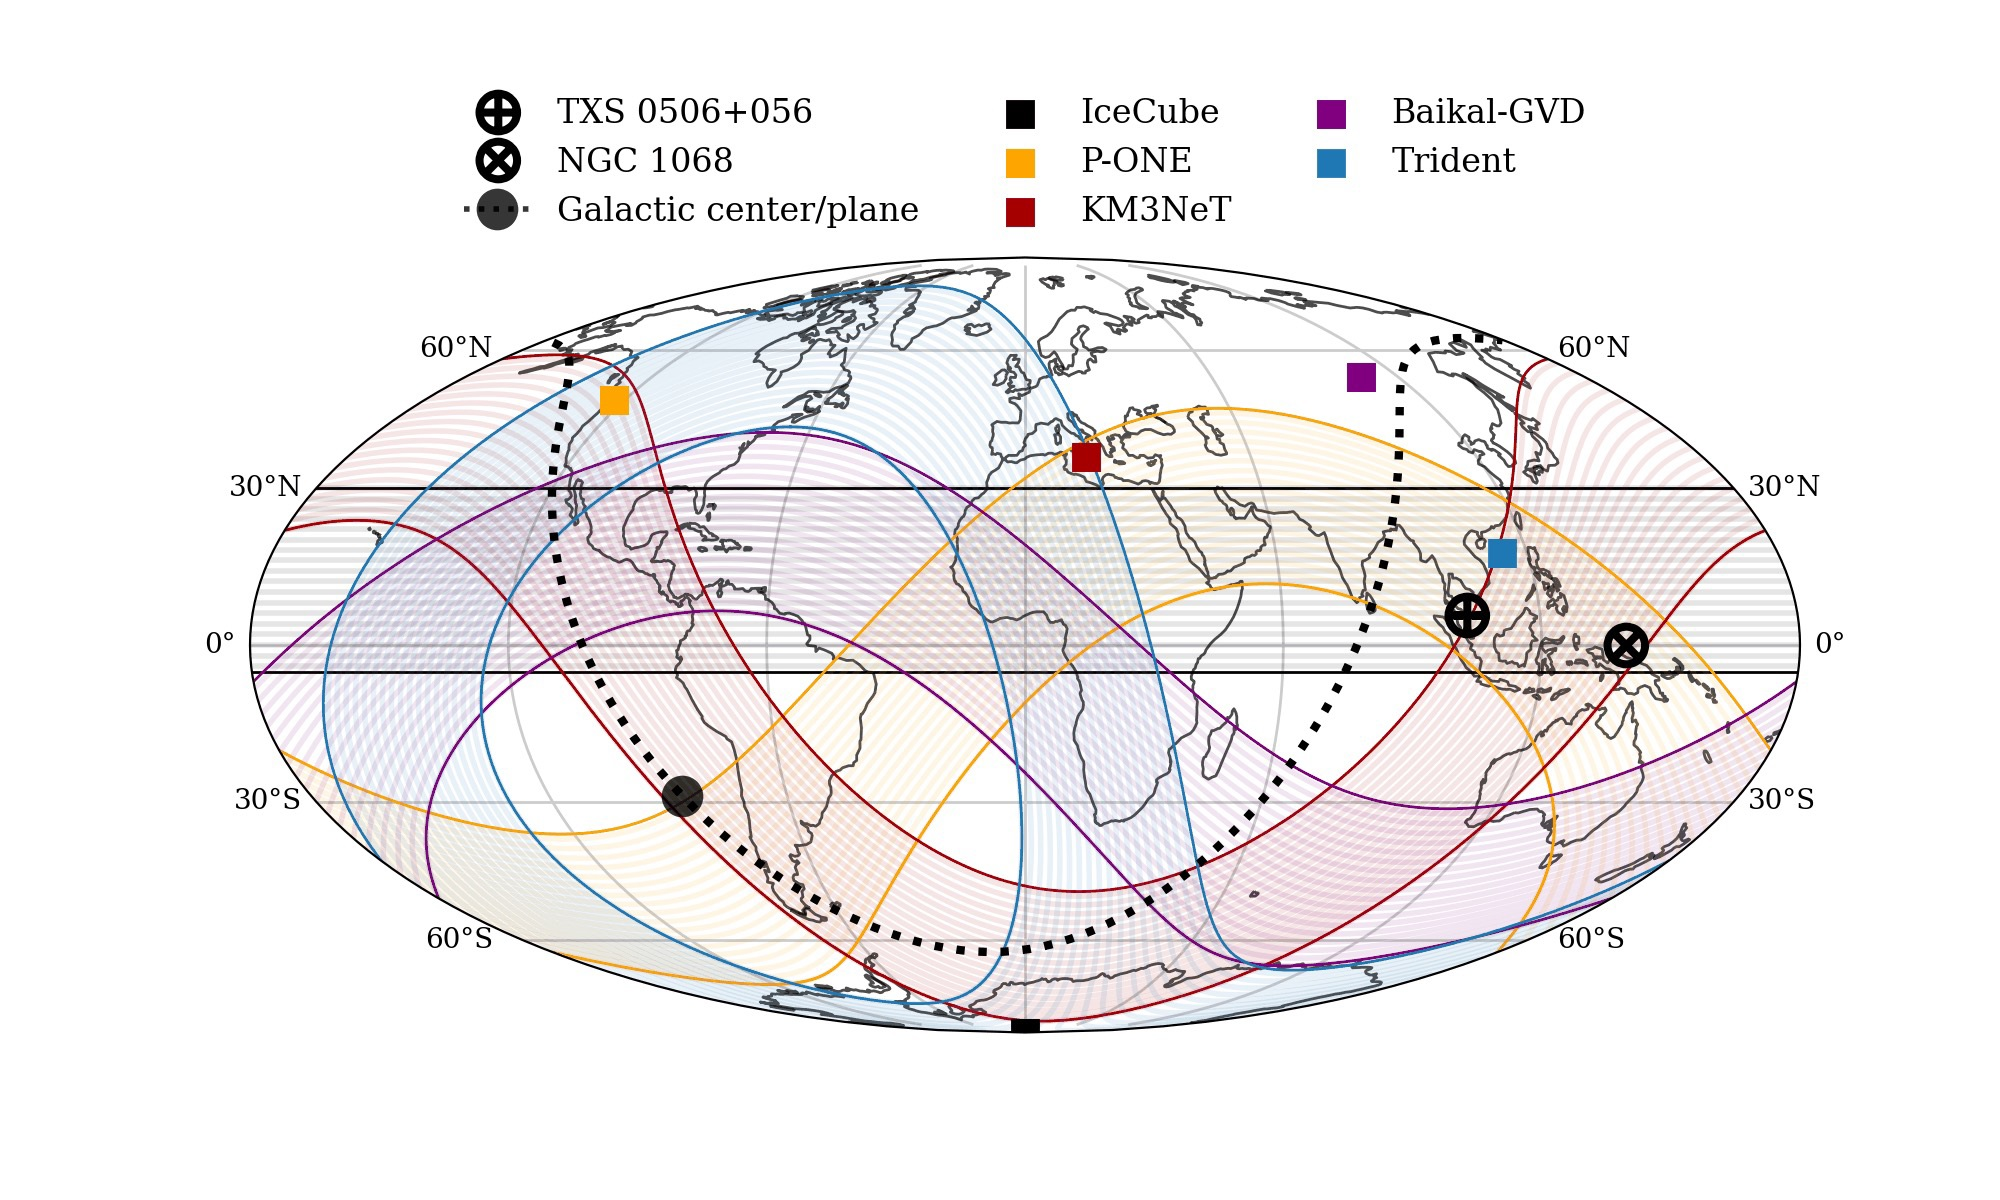
\includegraphics[width=0.95\linewidth]{img/detector_poistion_and_sensitive_band.jpg}
    \caption{目前已经建成或者规划中的中微子望远镜的位置以及其灵敏带。图片由Lisa Schumacher制作,截取自报告\cite{LuLu_PeVPA:2022}}
    \label{fig:detector_poistion_and_sensitive_band}
\end{figure}


\subsection{其他因素}

除了上文中介绍的两点以外,还有其他地理和环境的因素会对中微子望远镜产生影响,例如:

\begin{enumerate}
    \item 海水深度。中微子望远镜依赖于海水来屏蔽日光和大气缪子背景。太阳光在$\sim 1\,\mathrm{km}$的深度之后便已经被完全屏蔽。而对于大气缪子背景而言,海水的厚度每增加$1\,\mathrm{km}$,大气缪子的流量便会下降约一个数量级\cite{atmos_muon_depth:1998}。此外海水的深度还会影响洋流和生物丰度等。

    \item 洋流流速和均匀性。洋流会使得中微子阵列中的串列单元的位置偏离预设位置,对串列单元的力学性能提出要求。通过海底声学系统,可以对DOM的位置进行$\lesssim 10\, \mathrm{cm}$级别的定位\cite{KM3NeT_acoustic_1:2022, KM3NeT_acoustic_2:2022, Baikal_acoustic:2021},从而消除一部分洋流的影响。洋流在阵列尺度上的均匀性也是需要考虑的要点。海洋的洋流存在中小尺度的涡旋结构(公里级到亚公里级)\cite{current_simulation:2017},这种涡旋可能会改变阵列的形状结构,甚至使串列单元之间发生缠绕。

    \item 生物丰度。深海鱼类会通过发出光信号来进行相互之间的交流,此外海水中的有机物大分子也会在受到扰动之后(例如随着洋流碰撞到DOM上)发出生物光\cite{biolumi_modeling:2021}。这些信号对于中微子望远镜来说是一大主要的噪声干扰\cite{ANTARES_biolumi:2021, Baikal_biolumi:2021}。
\end{enumerate}

\section{世界上的中微子望远镜}

\subsubsection*{DUMMAND}

DUMMAND\cite{DUMMAND:1992}是第一台正式地进行详细设计并投入建设的大型中微子望远镜。它选址于夏威夷岛附近$\sim 4 \,\mathrm{km}$深的海底,计划构建世界上第一个$\sim\mathrm{km}^3$级大小的光敏探测阵列,如图\ref{fig:DUMMAND}所示。然而受限于当时的海洋工程技术,DUMMAND-II项目在布放第一根串列单元便遇到了线缆通讯的故障,最终被美国能源部终止\cite{Telescope_history:2019}。
尽管没有成功建设成大型阵列,DUMMAND合作组在长达20多年的时间中,对中微子望远镜的探测原理,科学目标,工程设计等等内容都进行了充分的探讨,为后世其他中微子望远镜的建设奠定了基础\footnote{\url{https://www.phys.hawaii.edu/~dumand/dumacomp.html}}。

\begin{figure}[htb]
    \centering
    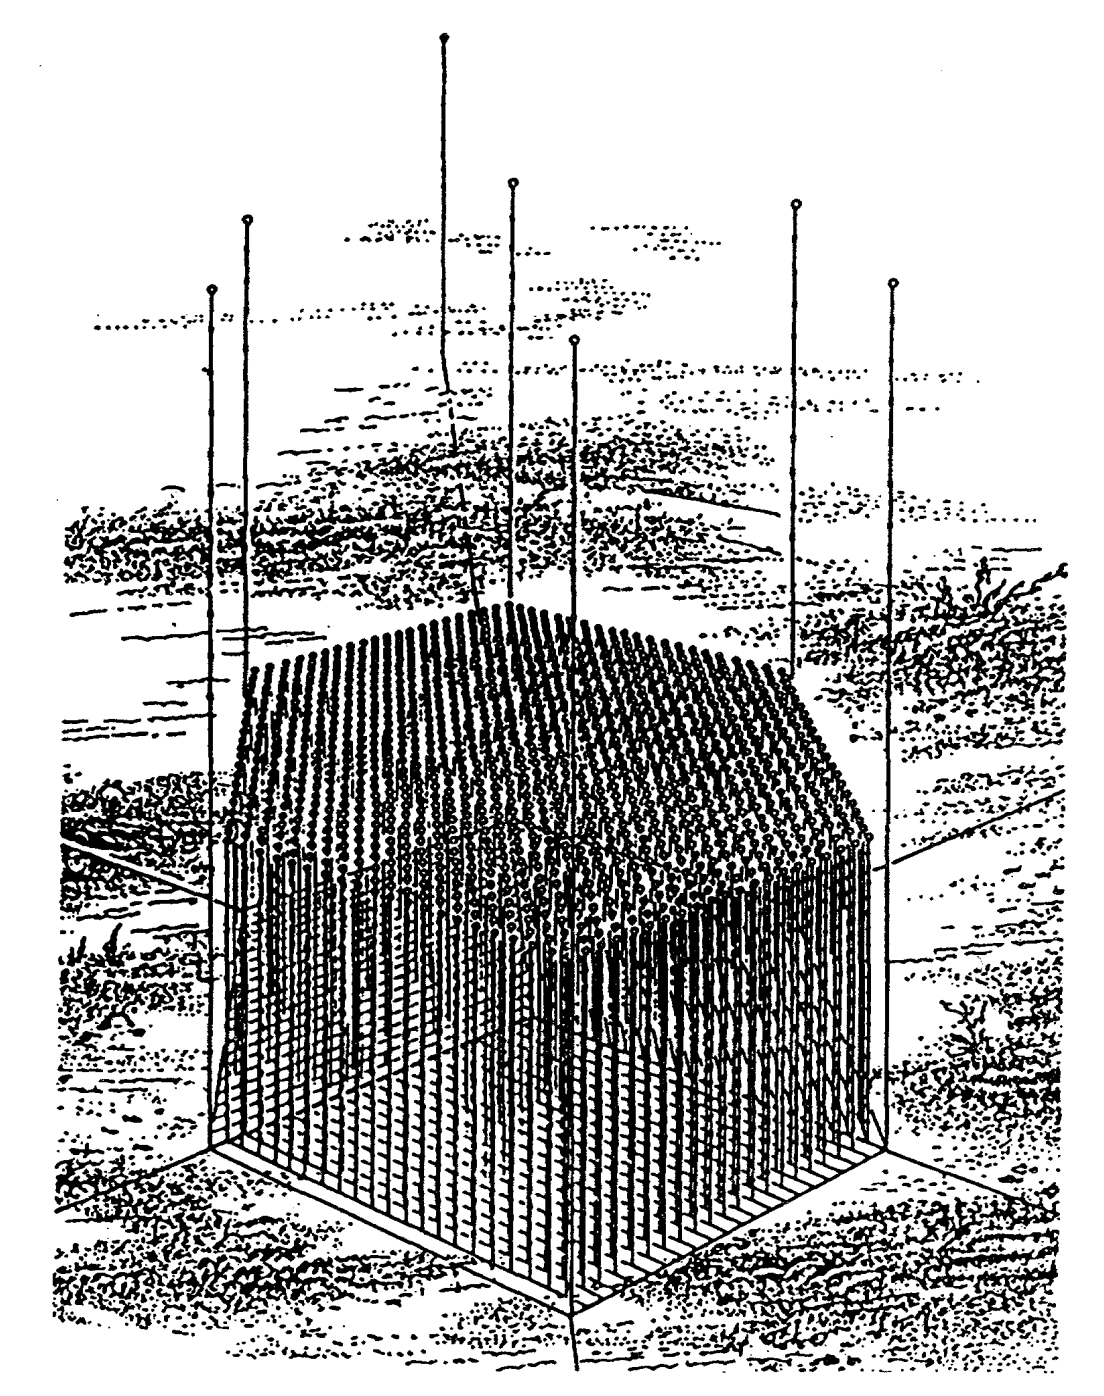
\includegraphics[width=0.7\linewidth]{img/DUMMAND.png}
    \caption{DUMMAND阵列设计图。图片来自\cite{DUMMAND:1992}}
    \label{fig:DUMMAND}
\end{figure}

\subsubsection*{AMANDA}

AMANDA\cite{AMANDA:1999}实验位于南极的冰川冰中,它成功地在$1150\,\mathrm{m}$~$2350\,\mathrm{m}$米的冰层中布置了约700个光敏探测阵列,如图\ref{fig:AMANDA}所示。
然而由于AMANDA的阵列规模较小,以及其光敏元件中缺乏数字化模块,AMANDA并没有找到高能的天体中微子信号\cite{AMANDA_neutrino_search:2007}。

\begin{figure}[htb]
    \centering
    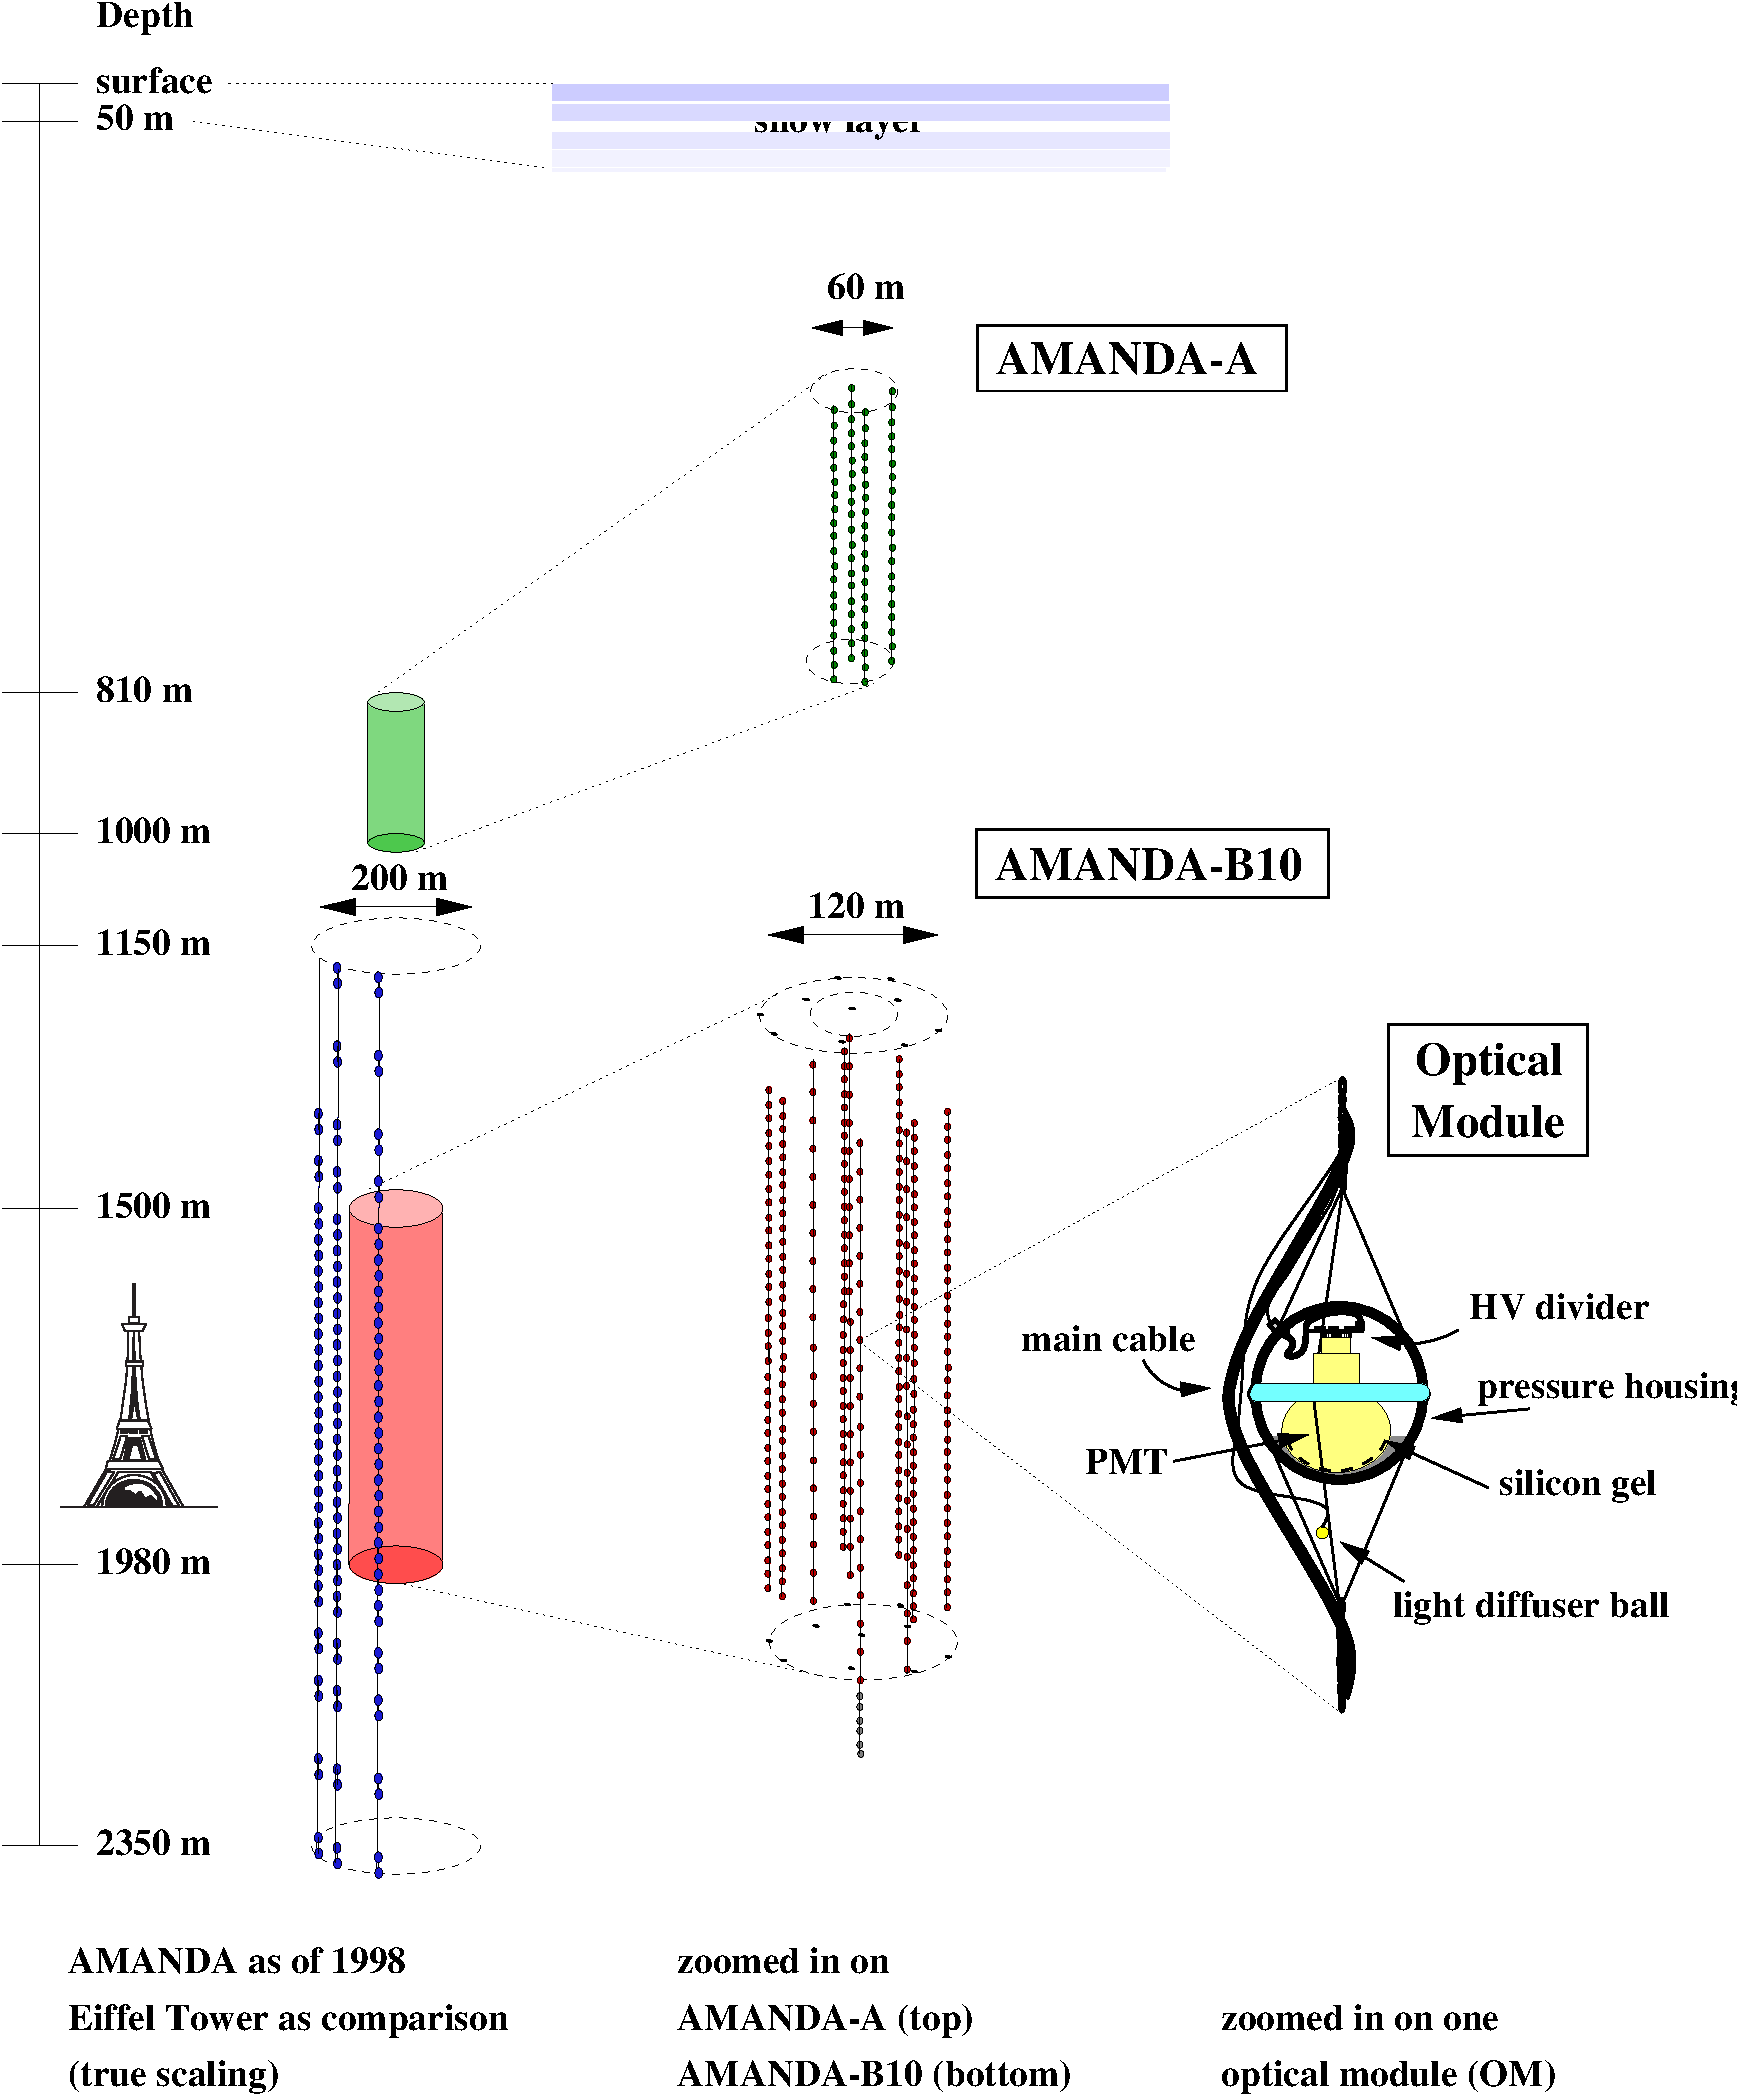
\includegraphics[width=0.8\linewidth]{img/AMANDA.pdf}
    \caption{AMANDA阵列设计图。图片来自\cite{AMANDA:1999}}
    \label{fig:AMANDA}
\end{figure}

\subsubsection*{Antares}

Antareas中微子望远镜位于法国南部2800米深的海水中,由约900个DOM组成\cite{ANTARES:2011}。
它是第一台真正建成的深海中微子望远镜,自2008年建成以来,它很多年的时间内保持了北半球最灵敏的中微子望远镜的地位\cite{ANTARES_highlights:2022}。
尽管没有显著地探测到高能的天体中微子,它的实验设计为后续的KM3NeT项目提供了不少经验。

\subsubsection*{IceCube}

IceCube是AMANDA的继承项目,它是世界上首个达到$1\,\mathrm{km^3}$体积的中微子望远镜,也是观测成果最为丰硕的望远镜\cite{IceCube_detector:2016}。IceCube在南极冰层下1450米到2450米之间布置了86根串列单元,每根上面挂载60个DOM,其阵列的示意图如图\ref{fig:IceCube_array}所示。
IceCube的阵列中DOM之间垂直间距为$16.7\,\mathrm{m}$,水平间距为$125\,\mathrm{m}$,这种悬殊的间距比例是由于IceCube在南极布置串列单元时需要支付昂贵的燃料费用于融化冰川冰。


\begin{figure}[htb]
    \centering
    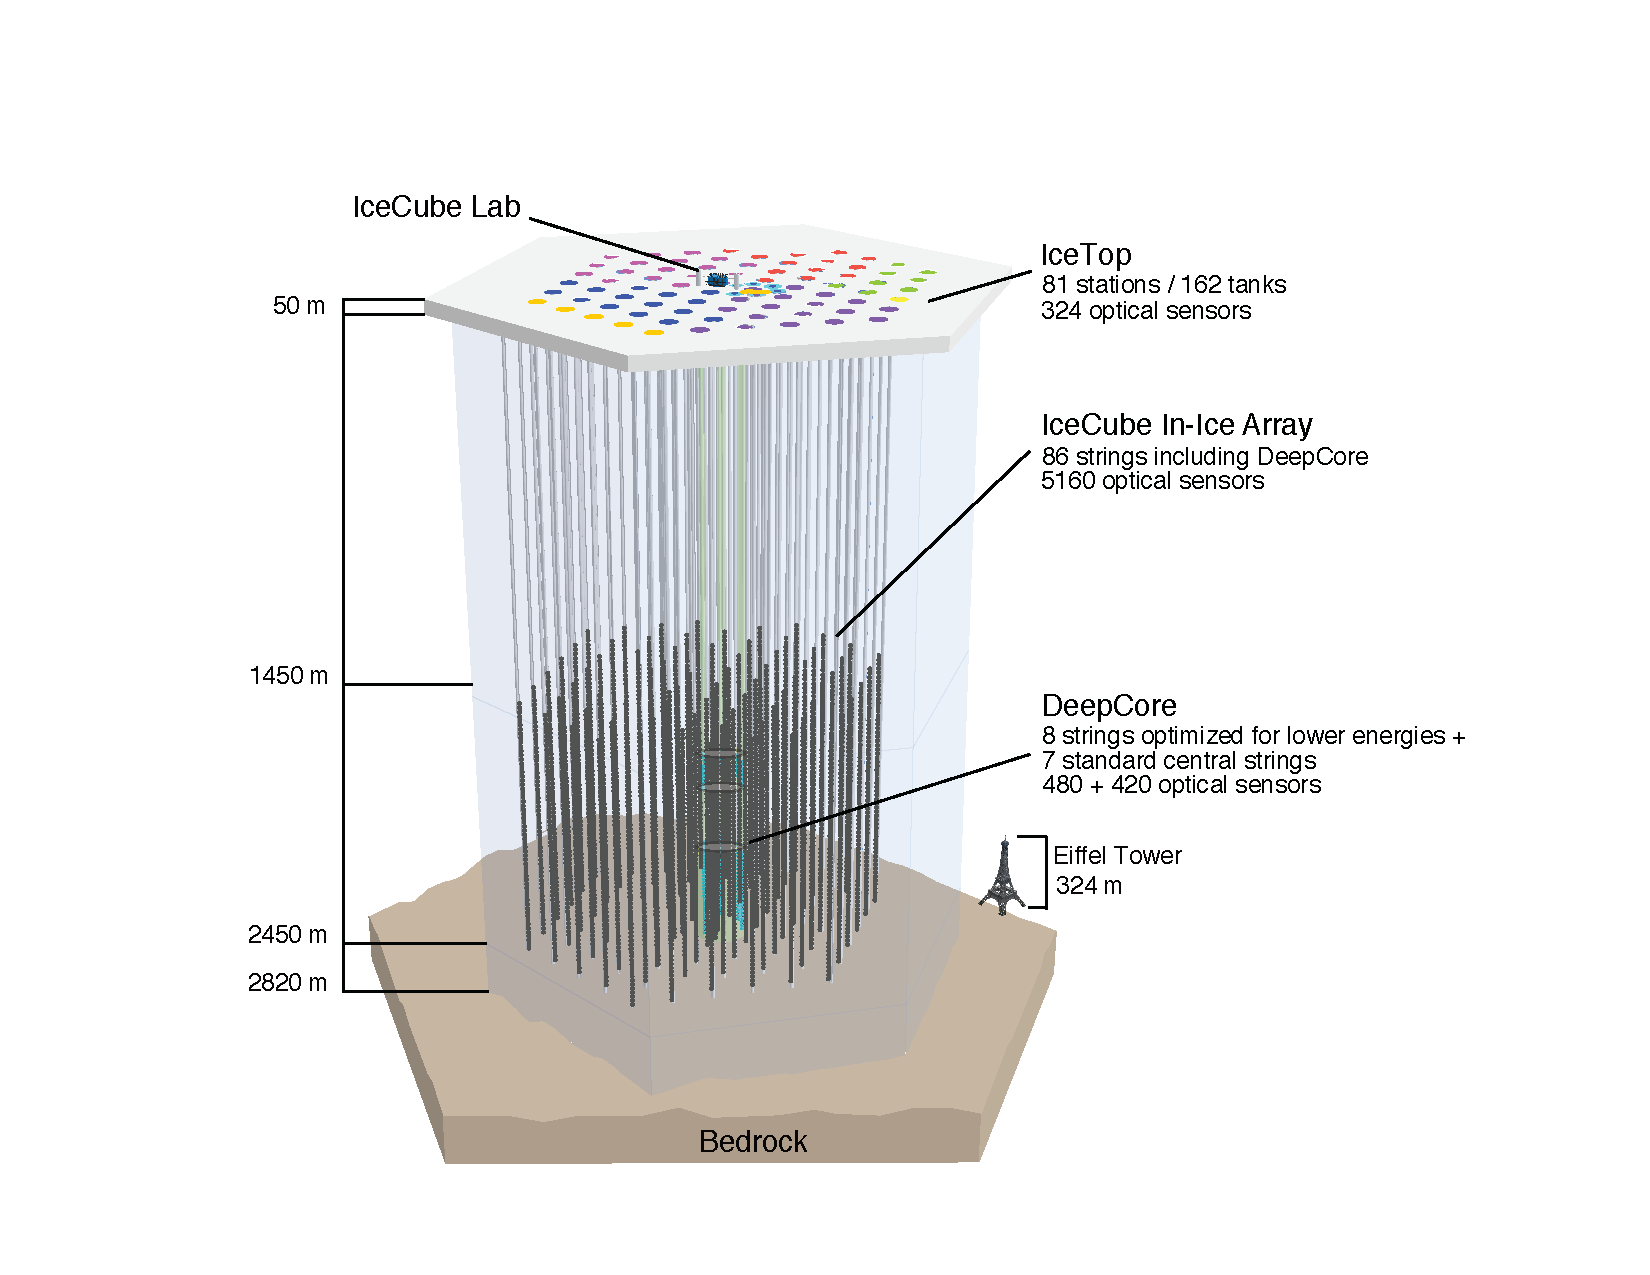
\includegraphics[width=0.8\linewidth]{img/IceCube_array.pdf}
    \caption{IceCube阵列设计图。图片来自\cite{IceCube_detector:2016}}
    \label{fig:IceCube_array}
\end{figure}

\subsubsection*{Baikal-GVD}

贝加尔湖是世界上最大的淡水湖,其水深可以达到$1500\,\mathrm{m}$,足以容纳一个中微子望远镜。贝加尔湖在冬季湖水表面上会结上一层超过1米厚的冰层,而在冰层上施工相比于大洋上施工会有诸多的便利。
贝加尔湖上曾经诞生过多个中微子望远镜项目,例如早期的NT-36,NT-200\cite{NT_200:1997},以及目前正在建造的Baikal-GVD\cite{BAIKAL_design:1997}。

如图\ref{fig:Baikal_scope}中所示,Baikal-GVD阵列由多个探测区块组成,目前已经完成了8个探测区块的建设,每一个探测区块之间的距离为$200\,\mathrm{m}$到$300\,\mathrm{m}$之间,其整体的监控体积达到$0.6\,\mathrm{km^3}$,是目前北半球最灵敏的中微子望远镜。
Baikal-GVD的每一个探测区块包含8根串列单元,形成一个半径$60\,\mathrm{m}$,高$525\,\mathrm{m}$的圆柱体。Baikal-GVD的每一根串列单元上包含了36个光敏元件,它们的深度位于$750\,\mathrm{m}$到$1275\,\mathrm{m}$之间。
这些光敏元件并不具备数字化的功能,而是将模拟信号传输到附近的专门用于数字化的球舱内来处理。

\begin{figure}[htb]
    \centering
    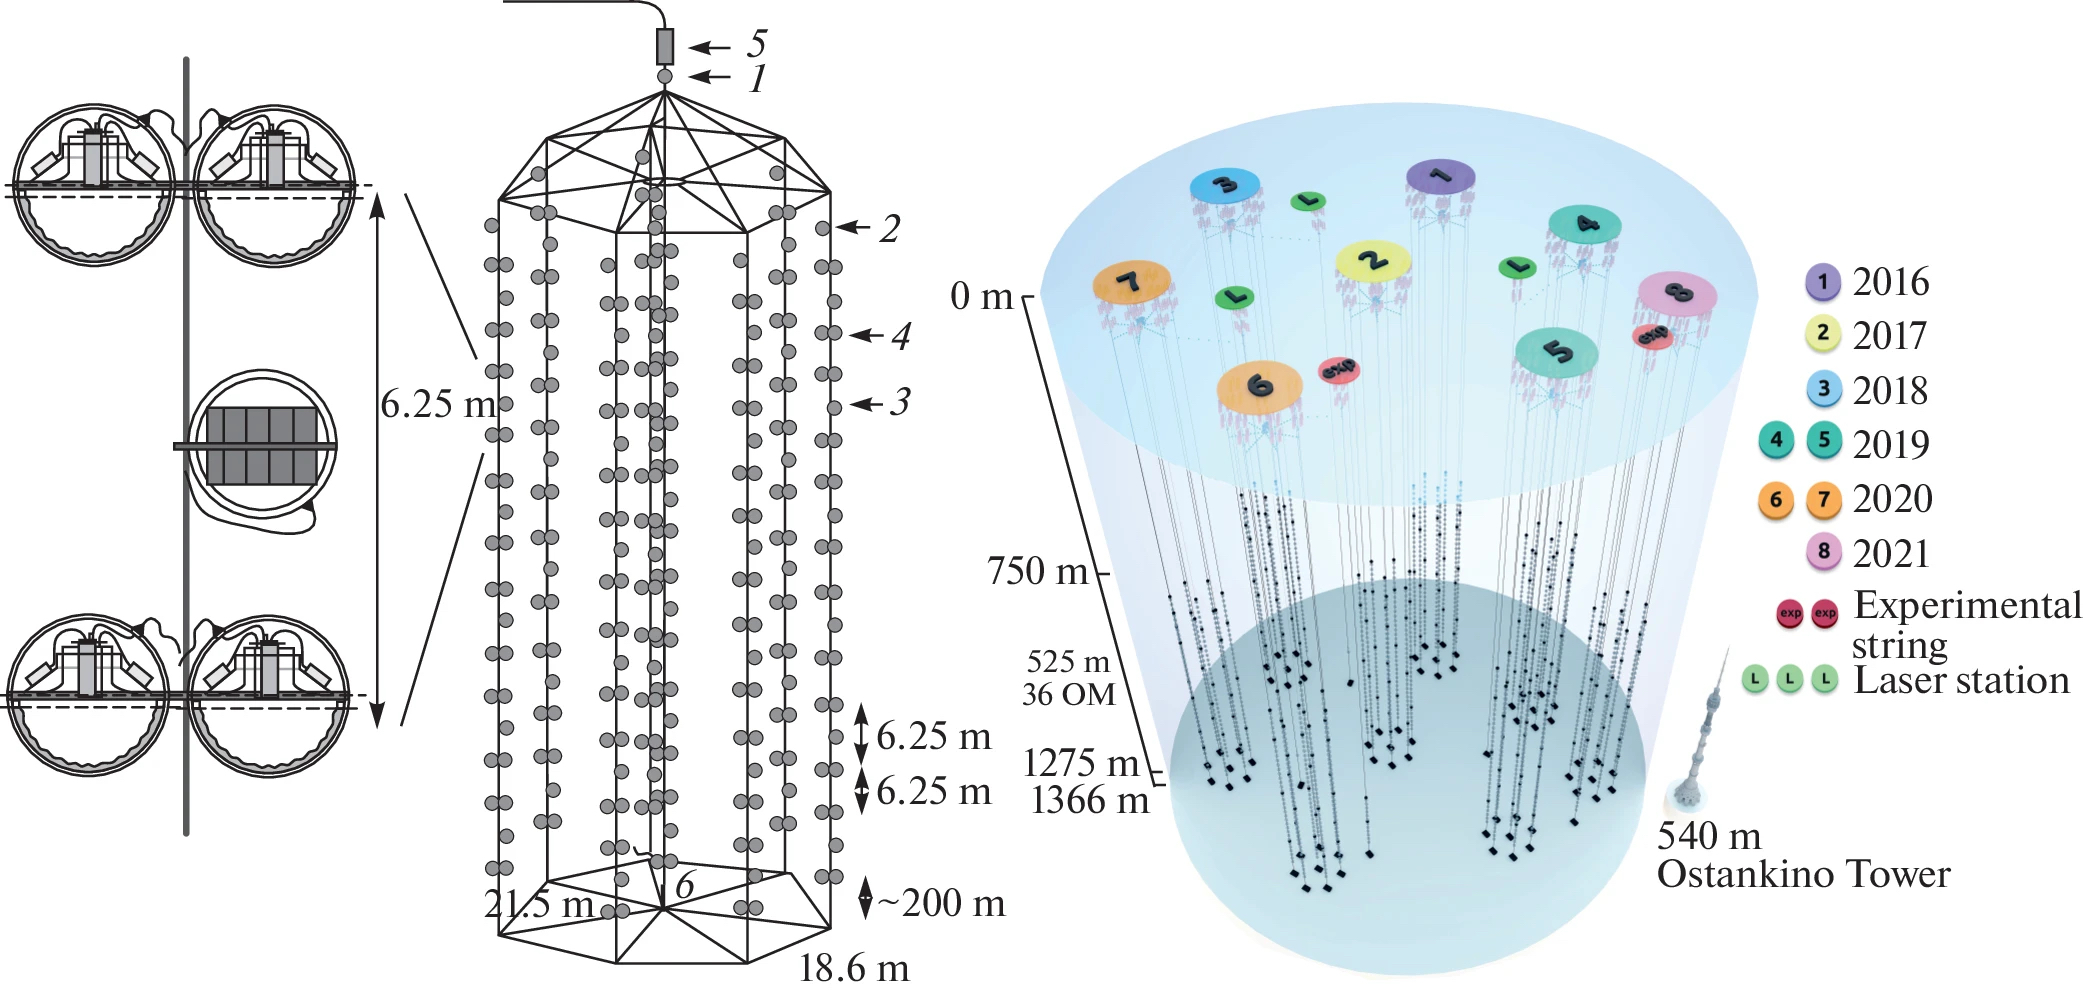
\includegraphics[width=0.8\linewidth]{img/Baikal_scope.jpg}
    \caption{左图,NT-200的探测器阵列示意图。右图,Baikal-GVD目前已经完成的阵列示意图。图片来自\cite{Baikal_status:2022}}
    \label{fig:Baikal_scope}
\end{figure}

\subsubsection*{KM3NeT}

KM3NeT是Antares的继承项目\cite{KM3Net_letter_of_intent:2016}。KM3NeT中包含两种不同的阵列构成,分别是排布更加稀疏针对高能天体中微子的ARCA,以及排布紧凑用于研究大气中微子振荡的ORCA。
KM3NeT-ARCA规划建设约$1.5\,\mathrm{km^3}$的阵列,目前已经布置了接近10根串列单元。

KM3NeT-ARCA中串列单元之间的平均间距为$90\,\mathrm{m}$,每一根串列单元包含18个mDOM,其间距为$36\,\mathrm{m}$。每一个阵列包含115根串列单元,形成一个半径为$500\,\mathrm{m}$,高度为$612\,\mathrm{m}$的圆柱形探测器阵列。
值得一提的是,KM3NeT中采用了一种独特的滚轮包装方式,可以将一根串列单元打包在一个大型滚球内,实现快速的布放\cite{KM3NeT_deployment:2020}。

\subsubsection*{P-ONE}

P-ONE(Pacific Ocean Neutrino Experiment)是一个正在计划设计中的,位于加拿大西海岸的中微子望远镜实验\cite{P-ONE:2020, P-ONE_ICRC:2021},它的阵列设计如图\ref{fig:P-One_array}中所示。
在目前的设计中,P-ONE类似于Baikal-GVD,由多个区块构成。P-ONE总共包含7个区块,每隔区块包含10根串列单元,每隔串列单元上挂在有20个光学探测模块。其区块和串列单元之间的几何间距如图\ref{fig:P-One_array}中所示。

相比于其他深海中微子望远镜,P-ONE的主要优势是它可以搭载在之前已经建设好的加拿大海底观测网(ONC,Ocean Networks Canada)\cite{P-ONE_ONC:2010},因此其海试实验和装置布放都相对比较容易。

\begin{figure}[htb]
    \centering
    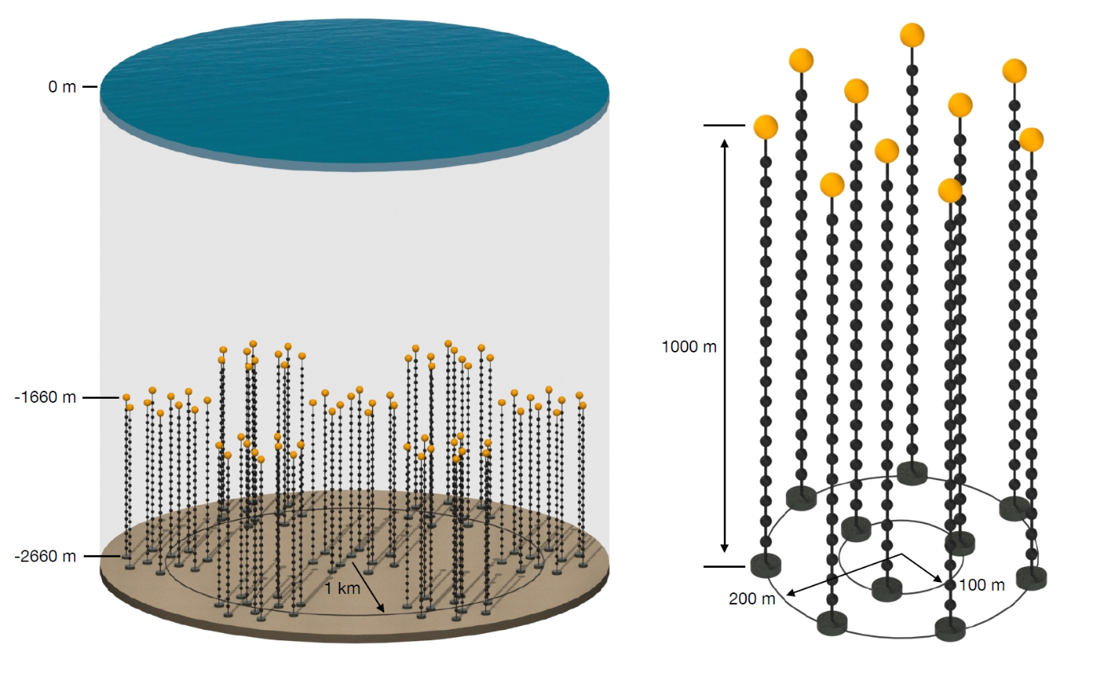
\includegraphics[width=0.8\linewidth]{img/P-One_array.png}
    \caption{P-ONE中微子望远镜阵列的概念设计图。图片来自\cite{P-ONE_ICRC:2021}}
    \label{fig:P-One_array}
\end{figure}


\subsubsection*{IceCube-Gen2}

IceCube-Gen2是计划中的IceCube的下一代升级版本\cite{IceCube-Gen2_white_paper:2020, IceCube-Gen2_VLVnT:2021}。它计划以几乎相同的DOM数量来覆盖$\sim5\,\mathrm{km^3}$的冰层体积,从而提高探测器的可观测能区。这是由于南极冰川冰中的吸收长度比较长,光子可以在冰内串行更长的距离。
在目前的设计中,IceCube-Gen2包含120根新的串列单元,串列单元之间的间距为$240\,\mathrm{m}$。每一根串列单元中包含80个DOM,其间距为$15.6\mathrm{m}$,从$1325\,\mathrm{m}$的深度延伸到$2575\,\mathrm{m}$。

除了光学阵列外,IceCube-Gen2还计划在上层冰盖上布置范围更广的射电观测阵列,它们可以用于监测超高能中微子事件中粒子簇射产生的射电信号\cite{IceCube-Gen2_radio:2021}。


\section{海铃中微子望远镜}
\label{sec:TRIDENT_array}

“海铃计划”旨在中国南海建设一座次时代的深海切伦科夫中微子望远镜——海铃中微子望远镜(以下简称为“海铃”),其英文名为TRIDENT(The tRoplcal DEep-sea Neutrino Telescope),其艺术图如\ref{fig:TRIDENT_array}所示。
海铃的地址位于永兴岛东北部的一片深海平原上,其水深约为$3400\,\mathrm{m}$,有关望远镜的选址调查可以参考\ref{chap:pathfinder}。

\begin{figure}[!htb]%
    \centering
    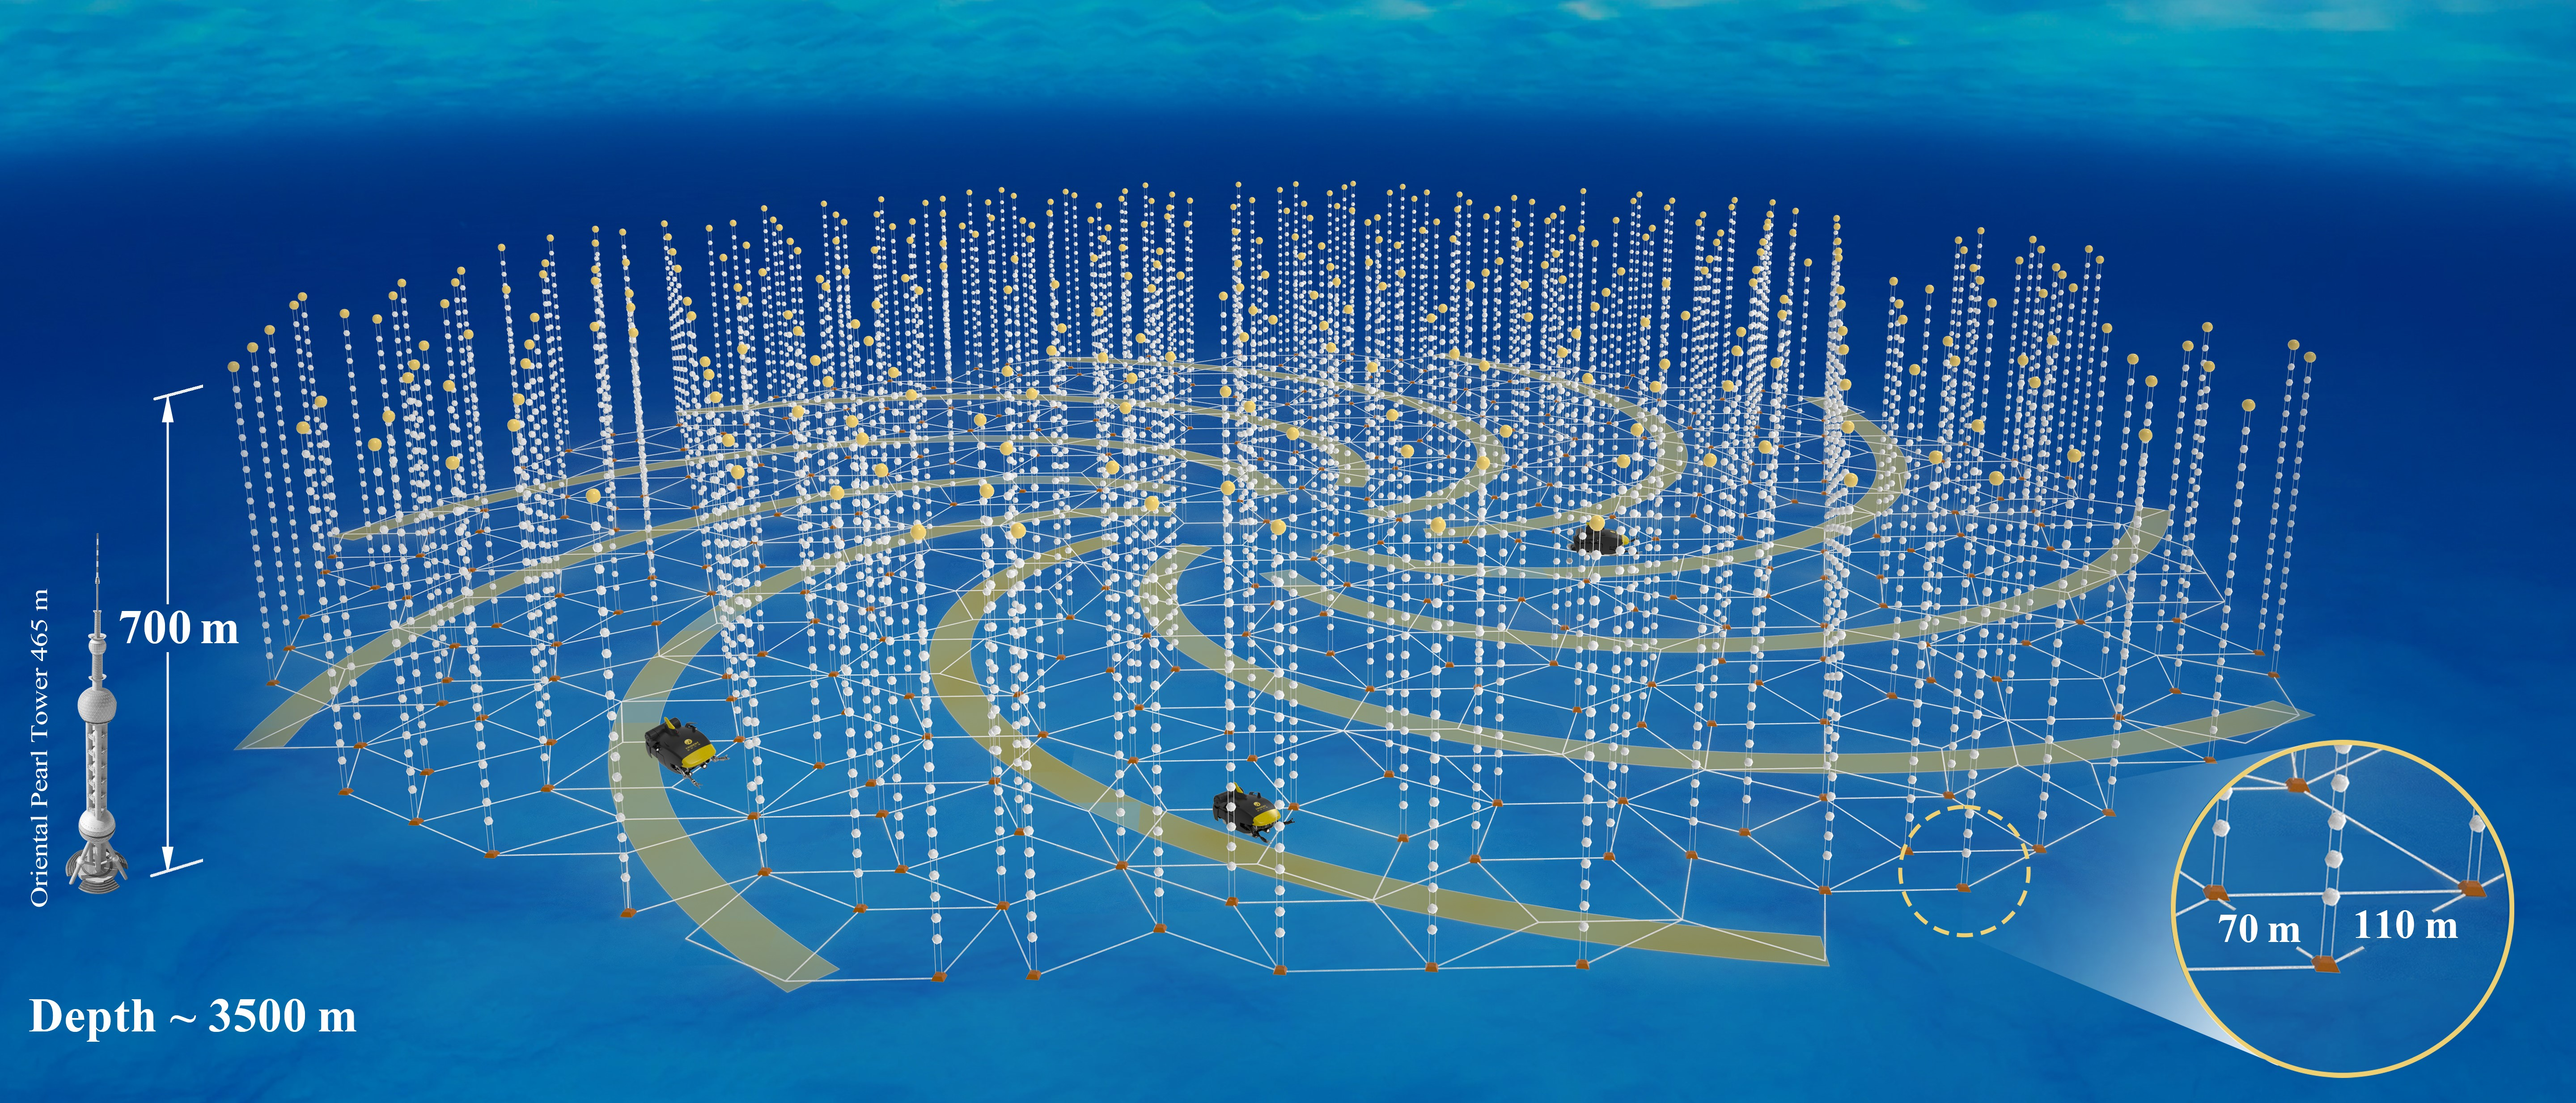
\includegraphics[width=0.95\textwidth]{img/TRIDENT_array.jpeg}
    \caption{海铃的艺术想象图。}
    \label{fig:TRIDENT_array}
\end{figure}

在目前的设计中,海铃采用了彭罗斯镶嵌的结构,其阵列结构如图\ref{fig:geo-layout}所示,图中的每一个黑点表示一根串列单元,图中总共916根串列单元。
这916根串列单元组成了一个半径约$2\,\mathrm{km}$的圆,其覆盖面积约$12\,\mathrm{km^2}$。
串列单元从海底(约3400米深)处延伸至水下2700米,其上分布有20个hDOM,它们之间的垂直间隔为30米,串列单元的高度约$0.7\mathrm{km}$。
海铃的光学探测器阵列的监控体积达到了$7.5\,\mathrm{km^3}$,是目前规划中的最大的次时代中微子望远镜。

在阵列中,我们考虑实际施工布放时的海洋工程要求,在阵列中间留下了一些空隙过道,如图\ref{fig:geo-layout}中虚线所示,我们称之为ROV过道。这些过道可以将探测器进行适当的分块,防止阵列排布过于紧密导致施工和后期维修困难,方便水下ROV机器人的运作。
为了避免缪子径迹型事件沿着直线直接通过过道穿过阵列而不触发阵列中的hDOM,ROV过道采取了螺旋线型的设计而非简单的直线设计。
需要注意的是目前这些ROV过道对阵列的影响尚未被考虑在模拟研究中,我们在阵列模拟中还是采用了无ROV过道的理想阵列排布,即总探测单元数量为完整的1211根,而非916根。

在阵列布局中,我们同样放置了一些海底次级接驳盒的布置点位,如图\ref{fig:geo-layout}中红色三角形所示。在目前设计的布局中,每一个次级接驳盒可以为附近的20根探测单元提供电力和数据传输的服务,但实际每个次级接驳盒可以供给的探测单元数量由主接驳盒到次级接驳盒的数据传输带宽和供电功率上限决定。

\begin{figure}[!htb]%
    \centering
    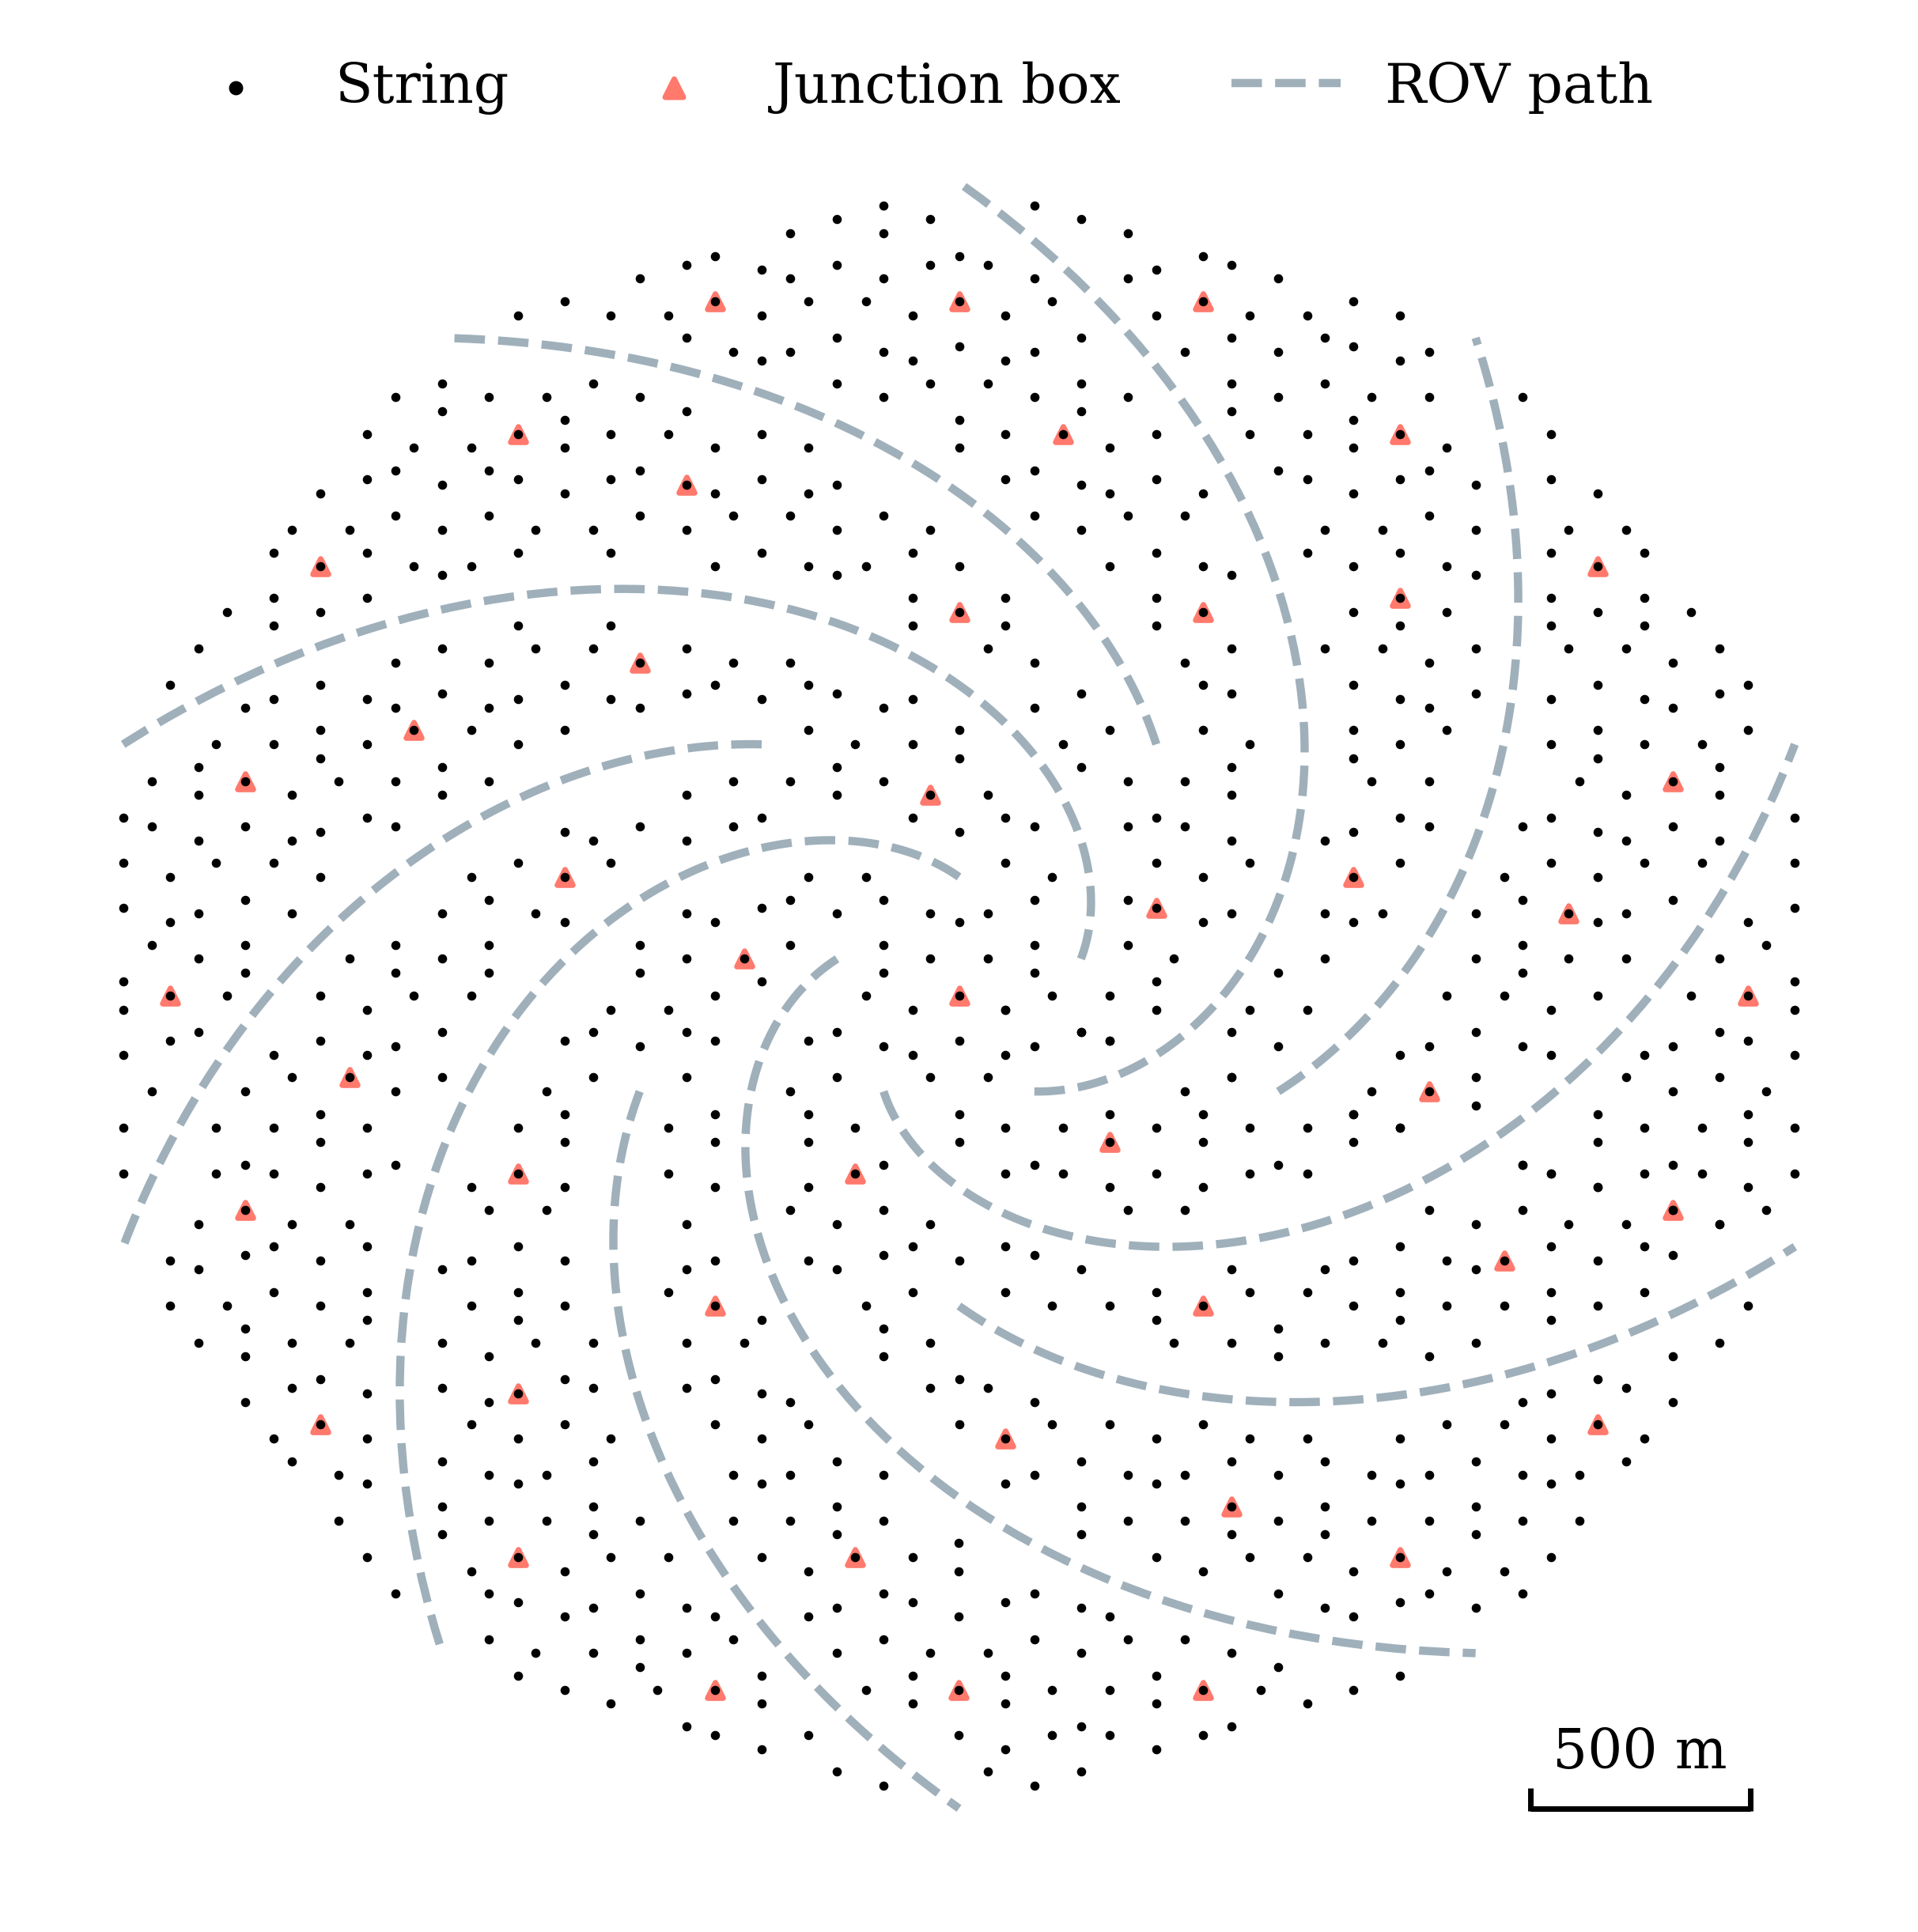
\includegraphics[width=0.85\textwidth]{img/penrose_tiling.png}
    \caption{海铃阵列的集合分布图,其中黑点表示串列单元,红色三角形表示次级接驳盒的位置,蓝色虚线表示ROV过道。}
    \label{fig:geo-layout}
\end{figure}

海铃的主要科学目标是从IceCube观测到的各向同性的弥散高能中微子流寻找产生它们的天体源。海铃庞大的探测器体积为中微子的事例率提供了保障,其优秀的角分辨率可以提高搜寻的灵敏度,有关海铃寻找中微子天体源的性能研究可以参考\ref{chap:telescope_performance}。
其次,海铃还能够研究天体物理尺度基线下的中微子振荡物理。为了实现这个科学目标,对不同中微子味道的分辨能力至关重要。
除了物理研究以外,海铃还是一个多学科研究平台,依托海铃搭建的海底光电缆网络可以布置地球物理和海洋生物研究的探测器。


    \chapter{中微子探测器的模拟框架}
\label{chap:simulation_framework}

对高能中微子的反应以及其探测过程的模拟是极其复杂的,因为其中包含多种不同能量尺度的物理过程::初始中微子和DIS顶点产生的主要次级粒子在在$\mathrm{TeV} - \mathrm{PeV}$量级,簇射演化时发生的级联过程会产生大量的$\mathrm{MeV} - \mathrm{GeV}$能级的次级粒子,而这些带电粒子产生的切伦科夫光子在$\mathrm{eV}$量级。
高能中微子反应与其探测过程中的各个粒子的自由程也各不相同:初始中微子可以穿透整个地球,而其DIS反应引发的粒子簇射中的粒子在海水中的自由程大约为$1\,\mathrm{cm}$(低能电子)$-100\,\mathrm{cm}$(高能光子),形成的整个粒子簇射的大小大长约$10\,\mathrm{m}$,半径约$0.1\,\mathrm{cm}$(电磁簇射)$-10\,\mathrm{cm}$(强子簇射),缪子在海水中的传播可以延伸至约$1\,\mathrm{km} - 10\,\mathrm{km}$,切伦科夫光子的传播由光的吸收长度所限制,大约局域在$\lesssim 100\, \mathrm{m}$的范围内。
因此,我们将中微子事件和探测器响应的模拟过程分为多个不同的模块,每个模块负责处理一部分的物理过程。在下面的章节中,我们对各个模拟模块进行介绍。

\section{中微子事件产生器}
\label{sec:event_generator}

中微子事件产生器(event generator)为后续的探测器模拟注入初始粒子,它主要进行以下任务:
\begin{enumerate}
    \item 模拟中微子与原子核的DIS作用
    \item 模拟陶中微子的衰变过程
    \item 模拟粒子从望远镜阵列外传播到阵列的过程
    \item 进行带权重的重要性采样
\end{enumerate}

由于中微子事件产生器要处理的任务复杂,各个中微子望远镜的合作组都为自己的实验设计了一套对应的模拟程序,例如\textsf{ANIS}\cite{ANIS:2004},\textsf{gSeaGen}\cite{gSeaGen:2020},\textsf{LeptonInjector-LeptonWeighter}\cite{LeptonInjector:2020}等。
海铃合作组也同样设计了一套中微子事件产生器\footnote{\url{https://gitlab.com/hailing/event-generator}},它是基于\textsf{CORSIKA8}模拟框架\cite{CORSIKA8:2018, CORSIKA8:2022}实现的。
\textsf{CORSIKA8}是著名宇宙线级联过程模拟软件\textsf{CORSIKA7}\cite{CORSIKA7:1998}的C++重构版本,它具有更好的可拓展性,用户可以更为轻易地通过C++接口添加感兴趣的物理过程并添加形状更复杂的探测器。
借助于\textsf{CORSIKA8}模拟框架,我们得以实现了中微子事件产生器所要求的各项功能,并且在该模拟框架下制作的程序具有更好的模块化特点,便于后期的更新和维护。

事件产生器的输入为我们要采样的初始中微子的动力学范围,例如中微子的能谱和方向,以及感兴趣的探测器范围等。程序的输入配置以\textsf{json}的格式进行保存,方便用户查看和修改。
事件产生器最终的输出结果为一系列的\textsf{McEvent}类的对象,它类似于粒子物理中常用的\textsf{HepMC3}蒙特卡洛输出结果\cite{HepMC3:2019},包含粒子物理事件的顶点和产物的动力学信息。具体的来说,每一个事件中都包含初始中微子的信息,DIS反应得到的初始粒子的信息,把这里粒子传播到达探测器表面后得到的新粒子信息,以及该事件的权重。
输出结果目前是以\textsf{json}的格式保存,这样可以方便人类用户直接查看事件中的数据,并且具有很好的可拓展性,但缺点是空间和时间上的效率相比于二进制文件来说低很多。

\subsection{几何设置}

\textsf{CORSIKA8}模拟框架中支持几种基本几何体,如球形,长方体,圆柱体等。在设置了几何体的形状后,还可以为其设置原子组分,介质密度,电离能损等信息,用于支持后续的物理过程模拟。
我们在\textsf{CORSIKA8}中构建了一个地球的密度模型,并且在其中放置了一个圆柱形粒子探测区域,用于表示海铃中微子探测器,如图\ref{fig:corsika_geometry}中所示。
我们采用了PREM(preliminary reference Earth model)\cite{PREM:1981}来对地球的密度分布进行建模,其密度模型如图\ref{fig:prem}所示。
在此基础上,我们添加了一层$3.4\,\mathrm{km}$厚的海水包裹在地壳外围,用于表示海铃所在位置的海水深度。
海铃中微子探测器的粒子检测范围为一个半径$2500\,\mathrm{m}$,高度$1000\,\mathrm{m}$的圆柱体。当粒子进入该圆柱体之后,\textsf{CORSIKA8}将不再继续进行粒子传播模拟,而是将粒子保存下来,作为后续更为精细的探测器模拟的输入。

\begin{figure}[htb]
\centering
    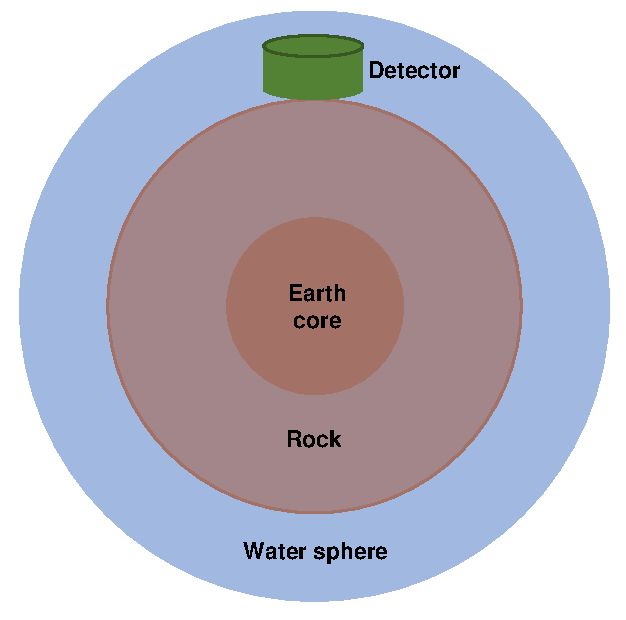
\includegraphics[width=0.70\textwidth]{img/corsika_geometry.pdf}
    \caption{模拟中的几何示意图。}
    \label{fig:corsika_geometry}
\end{figure}

\begin{figure}[htb]
\centering
    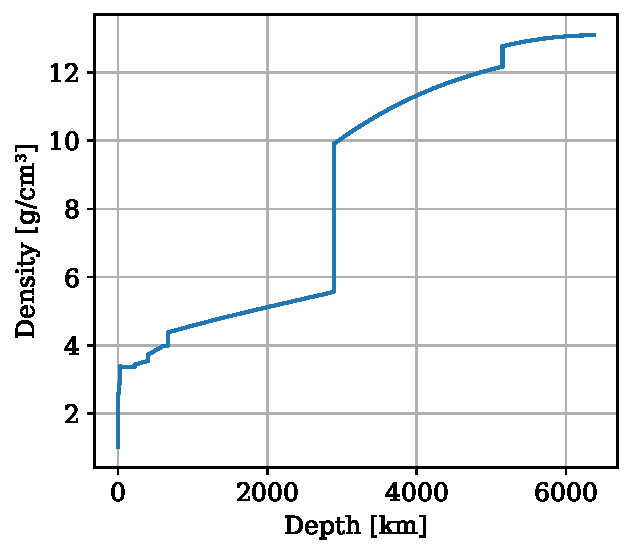
\includegraphics[width=0.60\textwidth]{img/prem.pdf}
    \caption{地球的密度模型。}
    \label{fig:prem}
\end{figure}

\subsection{DIS反应顶点的模拟}

在我们的模拟框架中,DIS和陶中微子的衰变过程都是通过\textsf{PYTHIA-8.3}程序\cite{Pythia8.2:2014, Pythia8.3:2022}实现的。
\textsf{PYTHIA}主要应用在大型强子对撞机(large hadron collider, LHC)中来模拟质子-质子碰撞后产生的结果,如图\ref{fig:event_generator_schem}所示。
除了强子-强子对撞模拟外,\textsf{PYTHIA}还可以处理轻子-轻子和轻子-强子对撞,以及粒子衰变的模拟。

\begin{figure}[htb]
\centering
    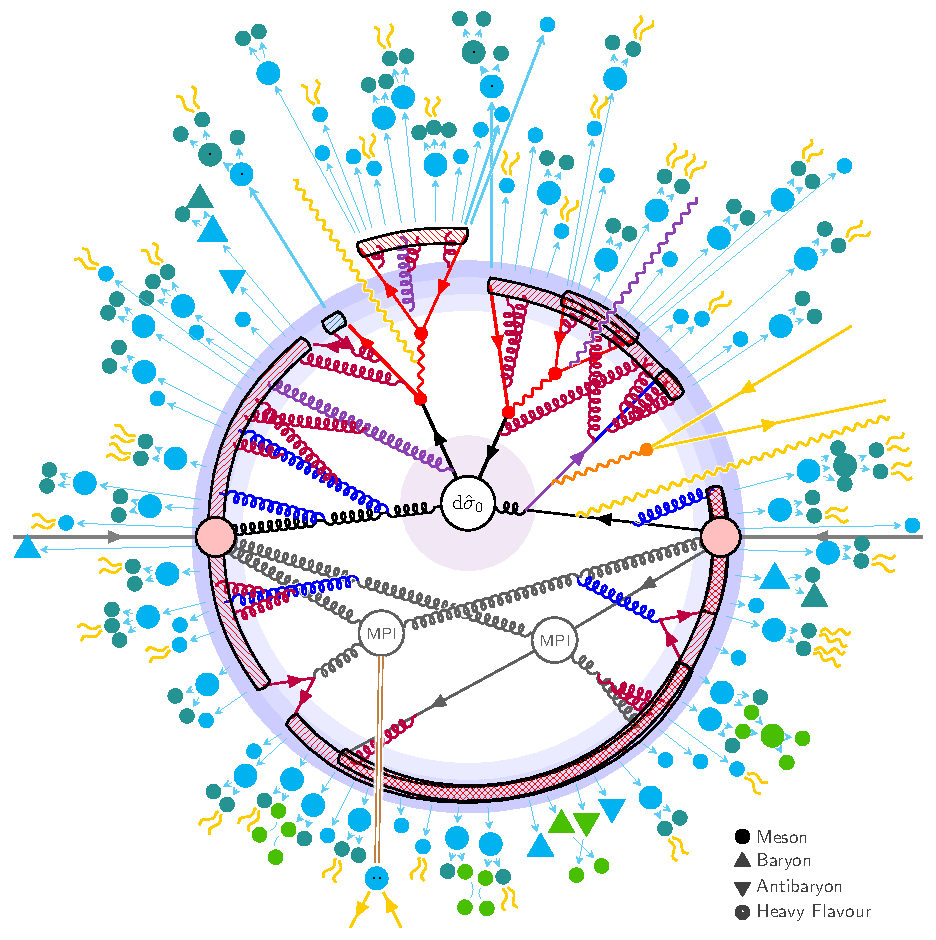
\includegraphics[width=0.73\textwidth]{img/event_generator_schem_fig.pdf}
    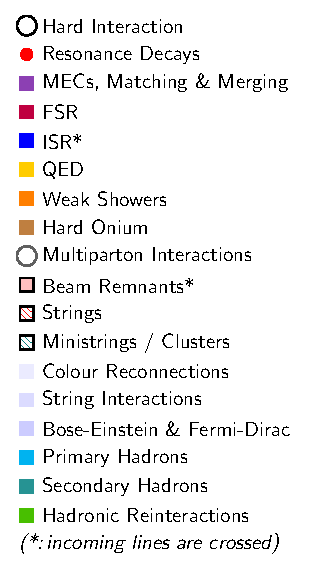
\includegraphics[width=0.25\textwidth]{img/event_generator_schem_legend.pdf}
    \caption{\textsf{PYTHIA}所处理的$pp\to t\bar{t}$事件的示意图。}
    \label{fig:event_generator_schem}
\end{figure}

用Pythia模拟中微子与原子核的DIS过程在Pythia程序内的反应分类中属于轻子-强子反应这一类别。在应用时,我们只需要打开Pythia程序中有关带电流相互作用的设置,再输入中微子的能动量信息以及靶粒子的信息,即可让Pythia进行DIS过程的模拟。
在我们的模拟框架中,我们在\textsf{CORSIKA8}中接入\textsf{PYTHIA}物理反应模块,将中微子传递到\textsf{PYTHIA}来进行DIS反应后,再将反应得到的粒子产物传回\textsf{CORSIKA8}中的栈堆,然后再进行后续的模拟。
通过Pythia模拟得到的$1\,\mathrm{PeV}$的电子中微子与质子发生DIS作用后得到的产物能量分布如图\ref{fig:DIS_product_energy_dist_primary}和\ref{fig:DIS_product_energy_dist_secondary}中所示。

\begin{figure}[!ht]
\centering
    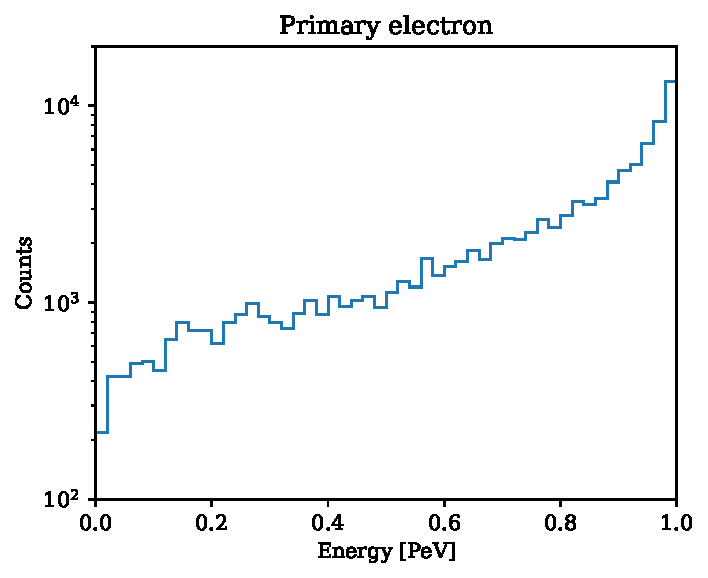
\includegraphics[width=0.60\textwidth]{img/DIS_primary_electron.pdf}
    \caption{在\textsf{Pythia}程序中模拟100k次$1\,\mathrm{PeV}$的电子中微子与质子发生带电流的DIS过程后,带电流作用中产生的主电子的能量分布图。}
    \label{fig:DIS_product_energy_dist_primary}
\end{figure}

\begin{figure}[!ht]
\centering
    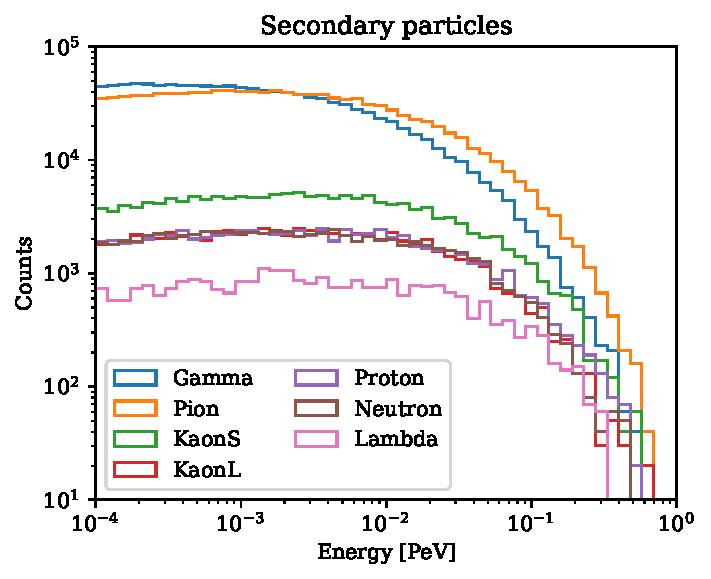
\includegraphics[width=0.60\textwidth]{img/DIS_secondary_particles.pdf}
    \caption{在\textsf{Pythia}程序中模拟100k次$1\,\mathrm{PeV}$的电子中微子与质子发生带电流的DIS过程后,原子核碎裂产生的主要成分的分布。}
    \label{fig:DIS_product_energy_dist_secondary}
\end{figure}


\subsection{缪子中微子径迹型事件采样}
\label{subsec:muon_sampling}

缪子可以在海水中传播$\mathcal{O}(10\,\mathrm{km})$,因此在距离探测器较远处的位置发生的DIS产生的缪子同样有可能传播到探测器,形成径迹型事件。
此类事件的反应顶点位置和方向的采样比较复杂,我们采用类似IceCube中的模拟程序\textsf{LeptonInjector-LeptonWeighter}\cite{LeptonInjector:2020}的采样模式。

该采样模式大致分为以下几步:
\begin{enumerate}
    \item 根据一个感兴趣的中微子能谱$F_\mathrm{mc}(E_\nu)$来对中微子的能量进行采样,得到中微子能量$E_\nu$。
    \item 在$4\pi$的立体角中随机选取一个方向$\vec{n}_\nu$,该方向将作为中微子的方向。
    \item 以探测器的中心为圆心,$R_0=2500\,\mathrm{m}$为半径(半径等同于探测器的大小),$\vec{n}_\nu$为法线方向,构成的圆盘中,均匀地抽取出一个点$\vec{x}_{i}$来作为中微子的初始位置。
    \item 调用\textsf{Pythia-8.3}物理模块来模拟该中微子与原子核的带电流的DIS反应过程,得到反应的产物,其中将会包含一个高能缪子。
    \item 通过缪子能损公式,来估计缪子能量$E_\mu$所对应能传播的柱密度范围$X_\mu$。
    \item 朝着中微子方向的反方向$-\vec{n}_\nu$,发射一条射线,计算该射线上柱密度达到$X_\mu$的地方到射线原点的距离,记为$D_\mu$。该过程中将会涉及到地球的密度模型,如果当射线超出地球范围时柱密度已然没有达到$X_\mu$,则进行截断。
    \item 在以$\vec{x}_\mathrm{i}$为原点,$\vec{n}_\nu$为方向,长度范围为$(-D_\mu-D_0, D_0)$的线段上均匀抽样出一个点$\vec{x}_\mathrm{f}$,这个点将会被作为真实反应发生的点,中微子和此前DIS产生的粒子的位置都将被设置在该点处。其中$D_0 = 2500\,\mathrm{m}$是一个与探测器大小接近的量,这里我们要求上述构造的长度范围为$(-D_\mu-D_0, D_0)$的线段足以包含以$\vec{x}_\mathrm{i}$为原点,$\vec{n}_\nu$为方向所构造的直线与探测器的相交线段。同样的,此时如果有线段超出地球的范围,就会进行响应的截断。
\end{enumerate}

通过以上的采样过程,我们的采样范围足以覆盖所有能够被探测器探测到的径迹型事件的反应顶点和方向,而与此同时,我们也并没有浪费计算资源模拟过多的无法被探测器检测到的信号,这样的蒙特卡洛采样在计算性能上是相当优秀的。

该采样过程对初始中微子的能量$E_\nu$,方向$\hat{n}_\nu$,和反应的顶点位置$x_\mathrm{f}$这三个维度进行了采样,而且其中很多过程都是均匀采样的。
然而真实的物理过程在该三个维度上的分布并非如此,例如中微子在探测器附近的流量大小与其真实流量以及穿过地球的概率有关,中微子的反应位置分布与探测器附近的密度分布有关,等等。
为了将我们采样的结果与这些物理过程联系起来,我们需要引入采样权重的概念,这种带权重的采样过程称为重要性采样。有关权重的内容,我们将会在\ref{subsec:weightings}中详细讨论。

如上所述,我们的事件产生器模拟的结果便是一系列的中微子DIS事件在探测器上的结果,以及对应的权重项。

\subsection{缪子传播模拟}

在此前的几节内容中,我们介绍了如何通过\textsf{Pythia8}来模拟缪子中微子与原子核的DIS过程,并且还介绍了如何采样这些DIS事件在中微子能量,方向和顶点位置这些相空间上的分布。对于缪子中微子通过带电流的形式发生的DIS作用而言,其产生的缪子可以传播公里到数十公里的量级。此时如果DIS顶点发生在探测器外,则需要将产生的缪子传播到探测器,即进行缪子传播过程的模拟。

在我们的模拟框架中,我们采用\textsf{PROPOSAL}程序来模拟缪子和其他轻子的传播过程\cite{PROPOSAL:2013, PROPOSAL:2019}。
在传播经过$100\,\mathrm{m}$的海水时,不同能量的缪子损失的平均能量如图\ref{fig:muon_energy_loss}中所示,可以看到在$1\,\mathrm{TeV}$的能量以上时,缪子的能损是辐射形式主导的,即能损效率正比于自身的能量,其对应的物理过程主要包括韧致辐射,正负电子对产生和光核反应。
这种辐射形式的能损过程具有散射截面小,沉积能量的范围波动大的特点,其能损过程可以引发伴随的电磁簇射或者强子簇射,因此具有具有很强的不确定性。
图\ref{fig:muon_energy_loss_hist}展示了各个能量下缪子穿行$100\,\mathrm{m}$的海水时损失能量的分布,可以看到在极端的情况下,缪子可以将自身几乎全部的能量都沉积其中。

\begin{figure}[!ht]
\centering
    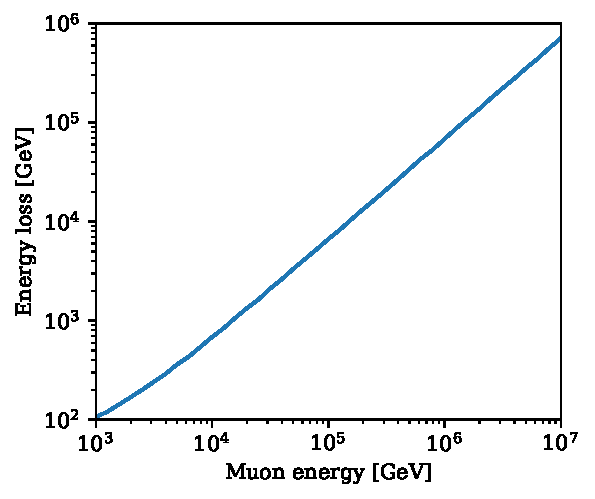
\includegraphics[width=0.55\textwidth]{img/muon_energy_loss.pdf}
    \caption{不同能量下,缪子穿行$100\,\mathrm{m}$的海水时的平均能损。}
    \label{fig:muon_energy_loss}
\end{figure}

\begin{figure}[!ht]
\centering
    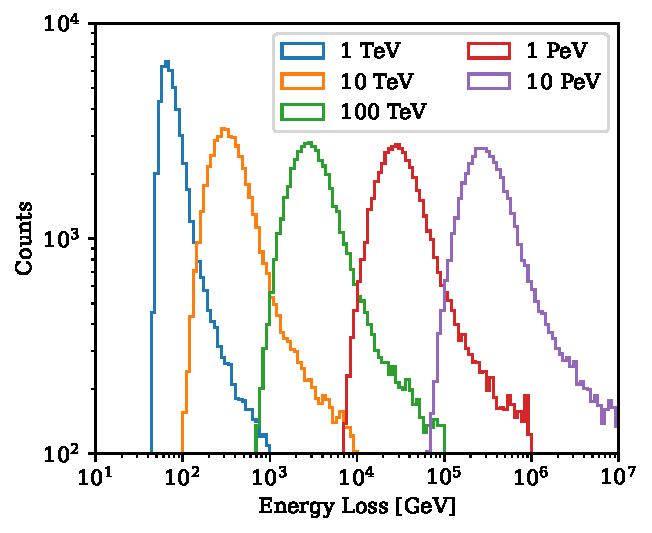
\includegraphics[width=0.60\textwidth]{img/muon_energy_loss_hist.pdf}
    \caption{不同能量下,缪子穿行$100\,\mathrm{m}$的海水时的能损分布。}
    \label{fig:muon_energy_loss_hist}
\end{figure}




\section{望远镜阵列内的粒子簇射模拟}
\label{sec:shower_simulation}

在使用中微子事件产生器生成探测器处能够接收到的粒子之后,我们将使用探测器模拟程序来继续模拟这些粒子的物理过程,进而得到真正对探测器而言能够探测到的物理信号,即光子在光敏元件上产生的光电子信号。

\subsection{高精度粒子物理过程模拟}

我们使用\textsf{Geant4}粒子模拟软件框架\cite{GEANT4:2003,GEANT4:2006}来对探测器内发生的粒子物理过程进行模拟。
\textsf{Geant4}中内置的物理库已经包含了从$\mathrm{eV}$到$100\,\mathrm{TeV}$能量范围内的绝大多数的粒子物理过程。
相比于\textsf{CORSIKA8},\textsf{Geant4}在低能范围内的物理准确性和计算效率都更为高效,而且其用户接口也更加丰富,适合进行详细的探测器内部模拟。

在我们的模拟中,我们将电子在海水中的簇射演化过程的动能阈值设置为$E_\mathrm{cut} = 0.25\,\mathrm{MeV}$,约等于电子在水中的切伦科夫能量阈值。这是为了保证所有能够产生切伦科夫光的粒子都被我们进行了模拟,确保事件的光产额不会丢失。


\subsection{通过参数化的方式加速簇射模拟}

电子在海水中主要通过韧致辐射和电离两种方式损失能量。其中韧致辐射过程将会发射光子,光子将会继续以康普顿散射的形式将能量传递给新的电子,由此实现了电子数量的倍增,即引发级联簇射过程。而电离过程会导致电子能量以热能的形式沉积在海水中,并在电子能量比较低时占据主要能损的地位。

在海水中,韧致辐射能损和电离能损的效率相同时的电子能量被定义为电子在海水中的临界能量(critical energy)\cite{PROPOSAL:2013}$E_c^e \simeq 0.1 \,\mathrm{GeV}$。\CHECK{CHECK THIS IN PROPOSAL}当电子能量高于$E_c^e$时将会发生级联簇射过程,而低于$E_c$时则不大可能会继续产生新的高能电子。
通过简单的计算,我们可以知道电子在海水中的簇射演化过程大约能产生的次级粒子数量为:
\begin{equation}
    N(E_0) \simeq E_0 / E_c^e
    \label{eq:param_flow_chart}
\end{equation}
其中$E_0$表示初始电子的能量。根据上述式子我们可以得到,对于约$100\,\mathrm{GeV}$的初始电子而言,其产生的次级电子数量可以达到$\sim 1000$个。
并且这些次级电子可以通过电离作用产生更多的低能电子,通过Geant4模拟中,我们可以统计到$\sim 20'000$个能量高于切伦科夫阈值($0.25\,\mathrm{MeV}$)的电子通过电离过程产生。
所有这些高于切伦科夫能量阈值的电子都可以辐射切伦科夫光子。

通过逐个粒子地方式模拟如此簇射演化中产生的大量的次级粒子将消耗不少的计算资源。在中微子望远镜中,几乎所有的电子级联过程都发生在空旷的海水中,因此簇射演化的过程实际上是比较稳定的。
图\ref{fig:param_num_photon_vs_energy}展示了电磁簇射中产生的总切伦科夫光子数与入射的电子能量之间的关系,我们可以看到他们之间存在如公式\ref{eq:emission_efficiency}中所描述的线性关系。
图\ref{fig:param_X_distribution}展示了电磁簇射的纵向发展,即产生切伦科夫光子的位置分布。
更多有关电磁簇射中物理量的分布和其拟合结果将在附录\ref{appendix:shower_param}中展示。

\begin{figure}[!ht]
\centering
    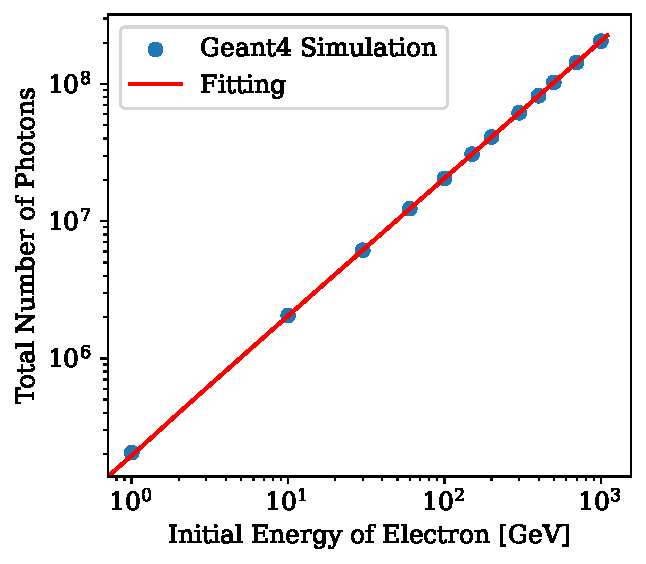
\includegraphics[width=0.65\textwidth]{img/param_num_photon_vs_energy.pdf}
    \caption{电磁簇射过程产生的总切伦科夫光子数与入射电子能量之间的关系图。}
    \label{fig:param_num_photon_vs_energy}
\end{figure}

\begin{figure}[!ht]
\centering
    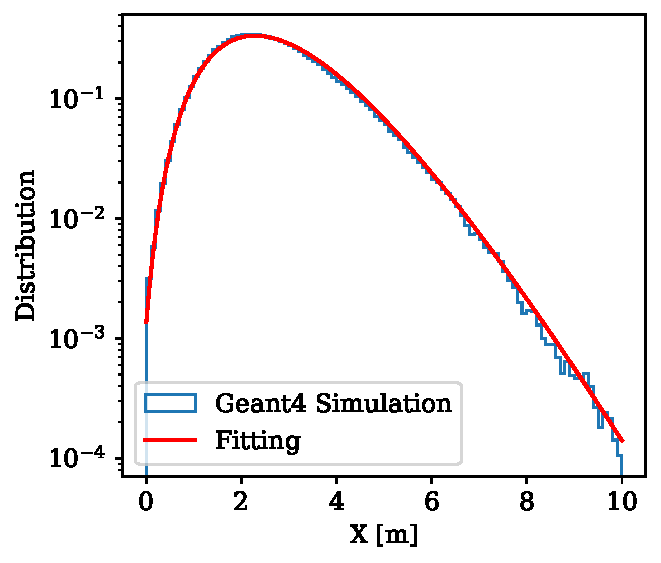
\includegraphics[width=0.65\textwidth]{img/param_X_distribution.pdf}
    \caption{电磁簇射过程中辐射切伦科夫光子的纵向分布。}
    \label{fig:param_X_distribution}
\end{figure}





通过对Geant4模拟实验的归纳总结,我们可以用参数化的方式来取代Geant4逐个粒子的模拟。
簇射过程参数化的程序结构示意图\ref{fig:param_flow_chart}所示。
考虑到中微子望远镜中实际的可观测量是切伦科夫光子,而切伦科夫光子是由带电粒子的轨迹所产生的,因此我们对电磁簇射演化过程进行参数化的目标便是快速得到一些能够产生切伦科夫光的轨迹,在我们的模拟中定义为\textsf{CherenkovStep},它包含带电粒子轨迹的运动信息(时间,位置,方向,速度)以及能够产生的切伦科夫光子的数量。
我们设计的级联过程参数化模块被嵌入到探测器模拟流程中,捕获能量在$1\,\mathrm{GeV}$到$100\,\mathrm{GeV}$能量范围内的电子,然后用参数化的方式将其快速转换为一系列的\textsf{CherenkovStep},从而取代标准的粒子物理模拟。

\begin{figure}[!ht]
\centering
    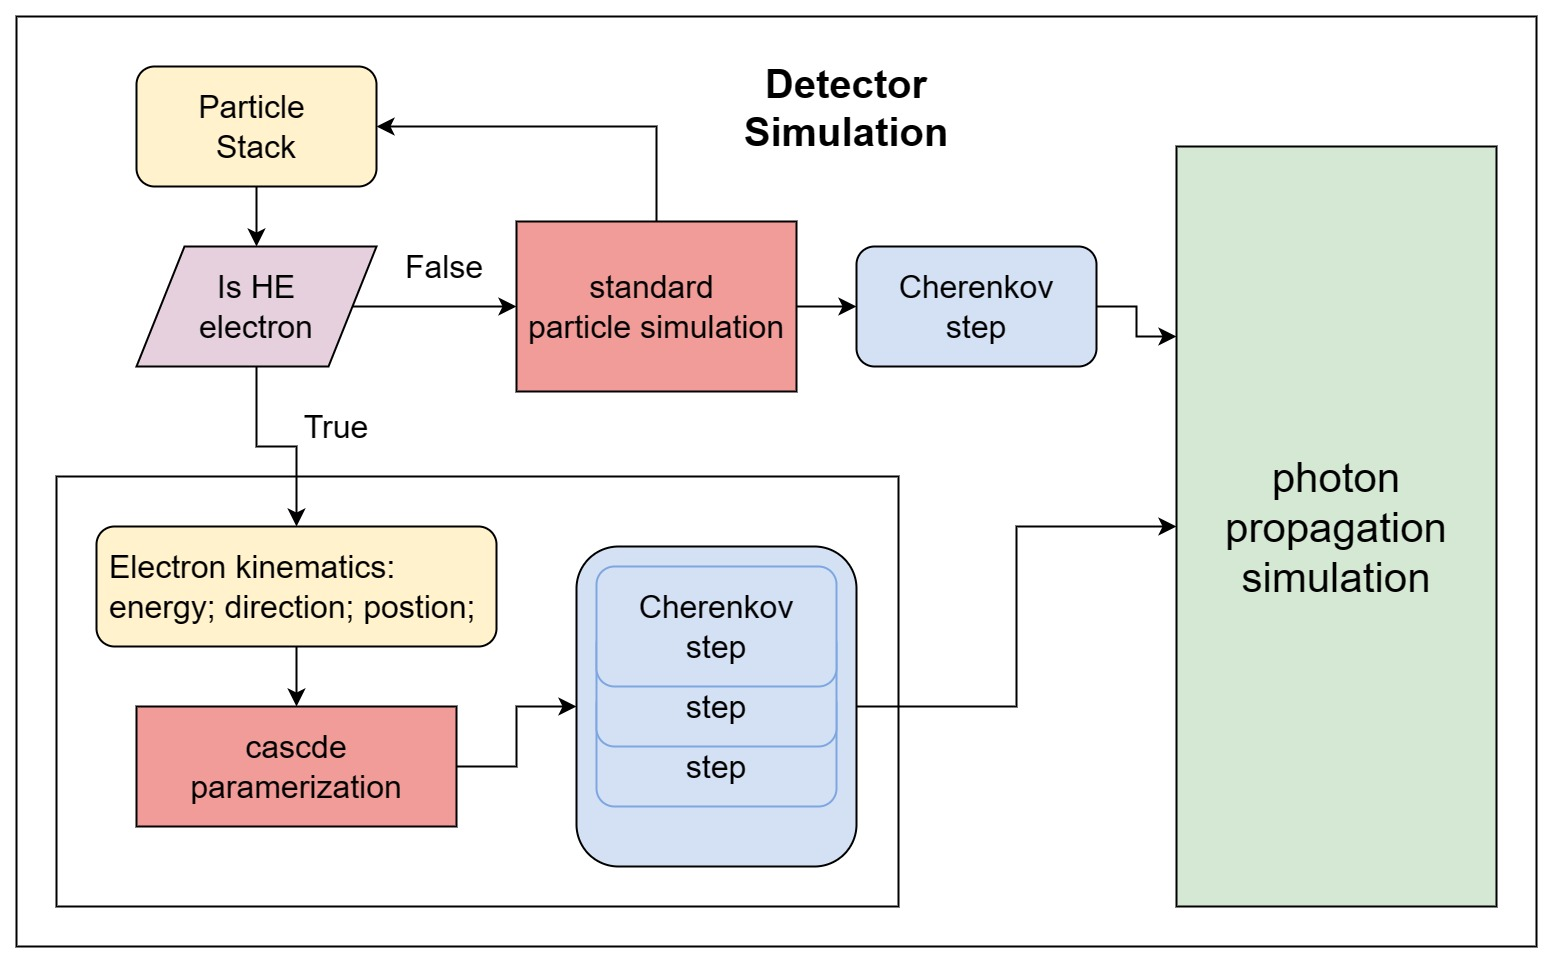
\includegraphics[width=0.95\textwidth]{img/param_flow_chart.jpg}
    \caption{簇射过程参数化的流程示意图。}
    \label{fig:param_flow_chart}
\end{figure}

\begin{figure}[!ht]
\centering
    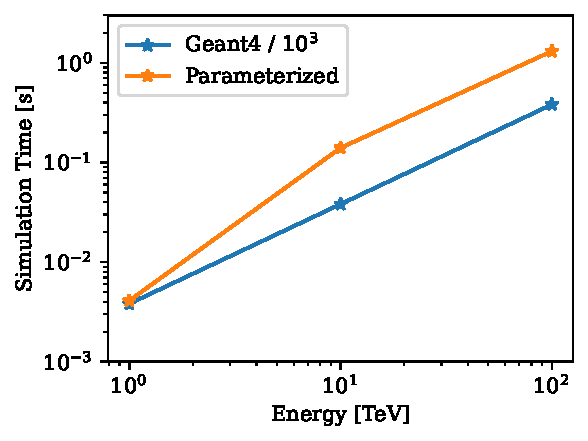
\includegraphics[width=0.65\textwidth]{img/performance_param.pdf}
    \caption{参数化的方式进行级联模拟与传统逐个粒子的模拟运行效率对比。}
    \label{fig:performance_param}
\end{figure}

通过参数化的方式进行级联模拟与传统逐个粒子的模拟运行效率对比如图\ref{fig:performance_param}所示。可以发现对于能量比较高的电子,以参数化的形式模拟之后,模拟速度有了$\mathcal{O}(1e^3)$倍的提升。

尽管簇射过程的参数化模拟无法做到和标准粒子物理流程得到的结果完全一致,我们的模拟研究表明,两者在光产额上的差距小于$1\%$,在DOM探测到的光子到达时间分布上差距小于$0.5\,\mathrm{ns}$。
这样的精度足以用于对中微子望远镜的性能研究,而参数化给模拟带来的性能提升是极其关键的,例如对于现代深度学习中的训练往往需要大量的模拟样本,只有使用参数化才有可能满足样本数量的需求。


\subsection{使用CORSIKA8来进行高能段的粒子过程模拟}

由于\textsf{Geant4}的强相互作用库只能进行实验室系下$100\,\mathrm{TeV}$能量的强子过程的模拟,不足以覆盖中微子望远镜中极高能部分的物理情形。
因此在将来的模拟框架中,我们将会使用\textsf{CORSIKA8}来代替\textsf{Geant4}来进行探测器内部的粒子物理过程模拟。
下面我们展示利用\textsf{CORSIKA8}来进行海水中的粒子级联过程的模拟结果


\section{切伦科夫光传播模拟}

\subsection{介质的光学性质模型}
\label{subsec:optical_model}

在介质中传播的电磁波会沉积能量并且激发介质中的电子,原子,分子和微小沉积物\cite{book_for_optical:1998}。
在激发的过程中,如果沉积能量高被转换成了热能的形式,那么便是发生了吸收过程,而如果沉积能量以再辐射的形式重新发光,则是发生了散射过程\footnote{本文仅讨论弹性散射过程,非弹性散射在海水中的影响非常小,因而可以忽略不计\cite{inelastic_scattering:2003}}。
尽管这种物理过程是以电磁波的形式加以描述的,根据波粒二象性,这些规律也可以描述微观光子的传播。

散射过程通常会被分为两种类型,分别是瑞利散射(Rayleigh scattering)和米散射(Mie scattering),他们的区别在介质中遮挡物颗粒的大小。
对于瑞利散射而言,介质中遮挡物的大小$r \ll \lambda$,其中$\lambda$是光子的波长。
而对米散射而言,遮挡物的大小和光子波长之间满足$r \gtrsim \lambda$。
在天然海水中,米散射主要是由有机物大分子贡献的,是主要的散射过程\cite{OP_ANTARES:2004, OP_Baikal:2012}。

散射过程对光子方向的改变可以用相函数$\beta(\cos\theta)$来描述,其中$\theta$即为光子的散射角。
对于瑞利散射而言,其相函数$\beta_\mathrm{Ray} (\cos\theta)$可以被偶极辐射模型来描述,并且辐射方向在入射光子的极化朝向和运动朝向上具有对称性。
米散射的模型描述会比瑞利散射更加复杂一些,这是因为米散射中颗粒物的大小并不能被忽略不计。米散射通常拥有非常尖锐的前向散射角。
人们通常用一个Henyey-Greenstein经验公式(以下简称为HG公式)\cite{Henyey_Greenstein:1941}来对米散射进行描述。
作为总结,上述对瑞利散射和米散射相函数的讨论可以分别被公式化为:
\begin{subequations}
    \label{eq:phase_function}
    \begin{align}
        \beta_\mathrm{Ray}(\cos\theta) &= \frac{3}{8} \left( 1 + \cos{\theta}^2 \right) \label{eq:pathfinder_phase_ray}  \\
        \beta_\mathrm{Mie}(\cos\theta) &= \frac{1}{2} \frac{1 - \mu^2}{(1 + \mu^2 - 2 \mu \cos{\theta}) ^{\frac{3}{2}}} , \label{eq:pathfinder_phase_mie}
    \end{align}
\end{subequations}
其中$\mu$是HG公式中的唯一参数,并且与$\cos\theta$的期望具有同样的值。

光子在介质中传播时,发生吸收,瑞利散射或者米散射的概率可以用平均自由程来表示,分别用符号$\lambda_\mathrm{abs}$,$\lambda_\mathrm{Ray}$和$\lambda_\mathrm{Mie}$来标记。
通常人们会额外定义衰减长度$\lambda_\mathrm{att}$:
\begin{equation}
    \frac{1}{\lambda_\mathrm{att}} = \frac{1}{\lambda_\mathrm{abs}} + \frac{1}{\lambda_\mathrm{Ray}} + \frac{1}{\lambda_\mathrm{Mie}} .
    \label{eq:pathfinder_attenuation}
\end{equation}

衰减长度可以用于描述如下的物理图像:当一束准直光在介质中传播时,无论是吸收还是散射,都会让光的辐射度(radiance,拥有能量每单位时间每单位面积每立体角的量纲)降低。
根据比尔朗博定律(Beer-Lambert law)\cite{Beer_Lambert_law:2020},准直光的辐射度$I_\mathrm{beam}(d)$随距离的衰减为:
\begin{equation}
    I_\mathrm{beam}(d) = I_\mathrm{beam}(0) e^{-d / \lambda_\mathrm{att}} .
    \label{eq:pathfinder_Beer_Lambert}
\end{equation}

另外一个经常被使用的物理量为散射角平均的吸收长度,定义为:
\begin{equation}
    \frac{1}{\lambda_\mathrm{att,avg}} \equiv \frac{1}{\lambda_\mathrm{abs}} + \frac{1}{\lambda_\mathrm{Ray}} + \frac{1 - \mu}{\lambda_\mathrm{Mie}} ,
    \label{eq:pathfinder_att_avg}
\end{equation}
该物理量考虑了一下物理图像:被前向散射的光通常对一大块的光照而言几乎没有影响。
因此,在一些对光子方向性要求没那么高的场合下(例如PMT对切伦科夫光的探测),$\lambda_\mathrm{att,avg}$可以用于近似得描述光照的整体衰减。关于$\lambda_ \mathrm{att}$和$\lambda_ \mathrm{att,avg}$之间的区别的详细讨论将会在章节\ref{sec:pathfinder_verification}中有更多地展开。

在我们的模拟程序中,我们使用的光学性质参数如图\ref{fig:optical_properties_in_simulation}中所示,其具体表达式如公式\ref{eq:optical_properties_in_simulation}和\ref{eq:refractive_index}中所示,其中我们并不区分米散射和瑞利散射对波长的不同依赖关系,而是先表示它们的总散射长度,然后用一个比例系数$r_\mathrm{Ray}=0.17$来表示瑞利散射在所有散射中的占比。
这些光学性质主要参考自KM3NeT中的模型\cite{Kopper:2010, Herold:2017},有关吸收长度的测量经过了海铃探路者实验的修正\cite{TRIDENT_pathfinder:2022},并且我们将米散射的参数$\mu$设置为0.93\cite{OP_Grace:2018}。

\begin{equation}
\begin{aligned}
    \frac{1}{\lambda_\mathrm{abs}} &= 
    360 * e^{-10 \times \frac{\lambda}{450}} + 
    3\times10^{-6} * e^{8.5 \times \frac{\lambda}{450}} \\
    \lambda_\mathrm{sca,eff} &= 
    8.78 \times \left(\frac{\lambda-300}{300} \right)^2 + 
    55.16 \times \left(\frac{\lambda-300}{300} \right) +
    18.49 \\
    \lambda_\mathrm{Ray} &= 
    \frac{\lambda_\mathrm{sca,eff}}{r_\mathrm{Ray}} \\
    \lambda_\mathrm{Mie} &= 
    \frac{\lambda_\mathrm{sca,eff}}{1 - r_\mathrm{Ray}}
    \label{eq:optical_properties_in_simulation}
\end{aligned}
\end{equation}

\begin{equation}
\begin{aligned}
    n_\mathrm{p} &=
    1.3236 + 16.257 \times \frac{1}{\lambda} - 
    4383.0 \times \left( \frac{1}{\lambda} \right)^2 + 
    1.1455 \times \left( \frac{1}{\lambda} \right)^3 \\
    n_\mathrm{g} &= 
    \frac{n_\mathrm{p}}{1 + \frac{\lambda}{n_\mathrm{p}} \frac{\mathrm{d} n_\mathrm{p}}{\mathrm{d} \lambda}}
    \label{eq:refractive_index}
\end{aligned}
\end{equation}


\begin{figure}[htb]
\centering
    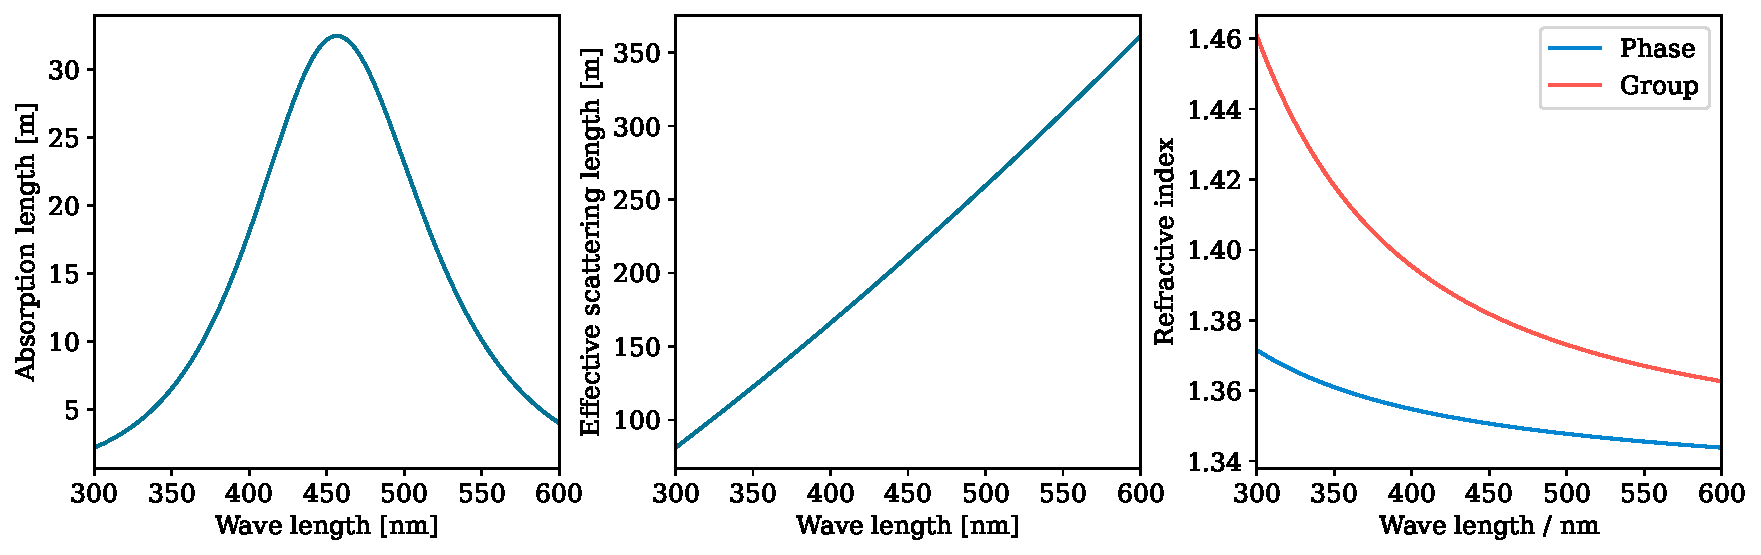
\includegraphics[width=0.95\textwidth]{img/optical_properties_in_simulation.pdf}
    \caption{光子传播模拟中所使用的光学性质参数。}
    \label{fig:optical_properties_in_simulation}
\end{figure}

\subsection{GPU加速的光线传播模拟}
\label{subsec:ray_tracing}

在第二章式\ref{eq:emission_efficiency}中,我们通过简单的估算得到了带电粒子在水中以切伦科夫光的形式辐射的光产额为$\sim 200\, \mathrm{MeV}^{-1}$。那么一个$1\,\mathrm{PeV}$能量的中微子事件如果将能量全部沉积在探测器监控体积内,将会产生$2 \times 10^{11}$个光子。
假设处理追踪一个切伦科夫光子的传播以及与探测器的碰撞需要$\mathcal{O}(10^3)$次的浮点运算次数,考虑现代CPU的运算频率为$\sim 3\,\mathrm{GHz}$,则对一个$1\,\mathrm{PeV}$能量的事件的模拟需要消耗的CPU资源为$\mathcal{O}(10^2) ~ \mathrm{core \cdot hour}$。
如此庞大的计算消耗是服务器集群所难以承受的。

光子在海水的传播以及与探测器的相交过程相比于其他粒子物理模拟在逻辑和运算结构上都是相对简单的,而且在粒子性的框架下不同的光子在传播的过程中并不会相互干扰。
对于这种逻辑简单且可以并行处理的任务而言,可以使用GPU来加速运算。
而且对于光线与物体的相交这种几何运算,在计算机图形学领域已经有大量的研究和现成的软件库可供使用\cite{RT_gems:2021}。
在高能物理领域,也存在不少使用GPU来加速光子传播的应用\cite{Dmitry_PPC:2013, Dmitry_PPC:2022, Opticks:2019, CORSIKA8_GPU:2021}。

在海铃探测器模拟中,我们基于\textsf{OptiX}光线追踪框架实现了GPU加速的光子传播模拟\footnote{\url{https://gitlab.com/hailing/hailing-optix}},其程序的结构图\ref{fig:RT_flow_chart}所示。

\begin{figure}[!htb]
\centering
    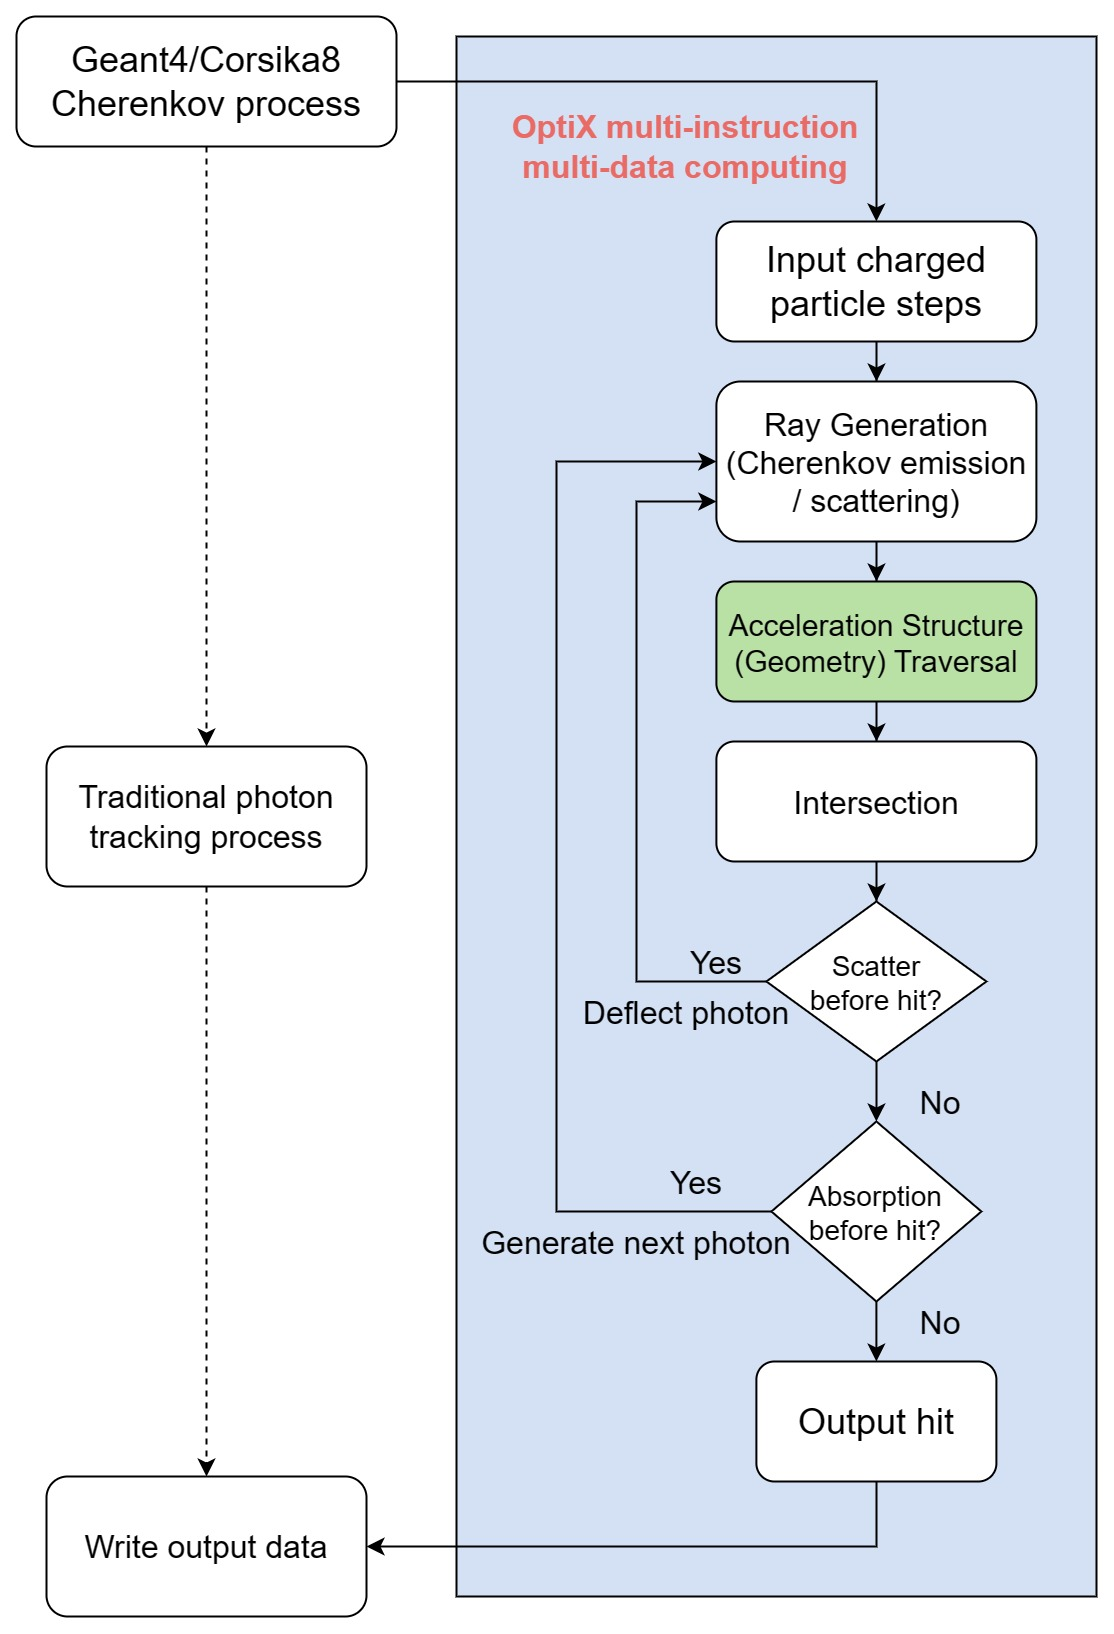
\includegraphics[width=0.75\textwidth]{img/RT_flow_chart.jpg}
    \caption{GPU加速的光子传播模拟的流程示意图。}
    \label{fig:RT_flow_chart}
\end{figure}

在光子传播模块中,我们首先将几何信息传递到GPU程序中。我们将探测器的几何简化为均匀的海水和一个个的DOM球。
光子传播模块从主探测器模拟程序中读取DOM球的几何坐标,并将这约20000个球的坐标位置按照位置的相邻关系构建成方便后续查询的几何加速结构(Acceleration Structure Traversal),从而方便快速地寻找光线与某一个球可能的交点。
海水介质在不同波长上的吸收,散射,折射率等信息被保存在了GPU显存中的材质图上,便于后续的查找和插值。

光子传播模块的输入为\textsf{CherenkovStep}的数组而非切伦科夫光子的数组。在程序中,每一个GPU线程都会各自处理一个\textsf{CherenkovStep}对象。
GPU线程将会根据\textsf{CherenkovStep}的时间,位置,方向,速度信息来不断地通过随机采样的方式产生并传播切伦科夫光子,直到达到该\textsf{CherenkovStep}中所应产生的光子数量。
采用这样的输入模式可以减少GPU显存与系统主存之间的通信开销,因为一个\textsf{CherenkovStep}便对应约1000个切伦科夫光子。
而在GPU计算中,数据传输所占用的时间往往大于真正浮点运算所占用的时间,即GPU计算通常是数据传输受限的(IO bound)\cite{CUDA_for_engineers:2015}。

根据\textsf{CherenkovStep}中的信息产生切伦科夫光子后,程序调用OptiX的光线追踪计算,来判断切伦科夫光子是否与几何体存在交点以及到交点的距离$d_\mathrm{int}$。
紧接着,程序将会根据介质的光学性质以及当前光子的波长来随机采样光子的吸收长度$d_\mathrm{abs}$,散射长度$d_\mathrm{sca}$。
接下来,光子会进行上述三个距离中最短的距离所对应的作用:如果是吸收则开始模拟下一个光子;如果是散射则将光子向前传播$d_\mathrm{sca}$的距离,随后根据散射的相函数改变光子运动方向;如果是相交则表示光子能够击中探测器的表面,我们会将光子在探测器表面的位置,运动方向,波长,以及探测器的ID记录到输出中。
每一个GPU中的线程负责处理一个\textsf{CherenkovStep}中产生的光子,它会不断循环直到将其中应当产生的光子都被处理完全。
此时如果粒子模拟中还有剩余的\textsf{CherenkovStep},则调度中心将会继续为空闲的线程分配新的\textsf{CherenkovStep}。



\section{hDOM探测器模拟}
\label{sec:hdom_sim}

\subsection{hDOM内部的光子传播模拟}
\label{subsec:hDOM_sim}

\begin{figure}[htb]
\centering
    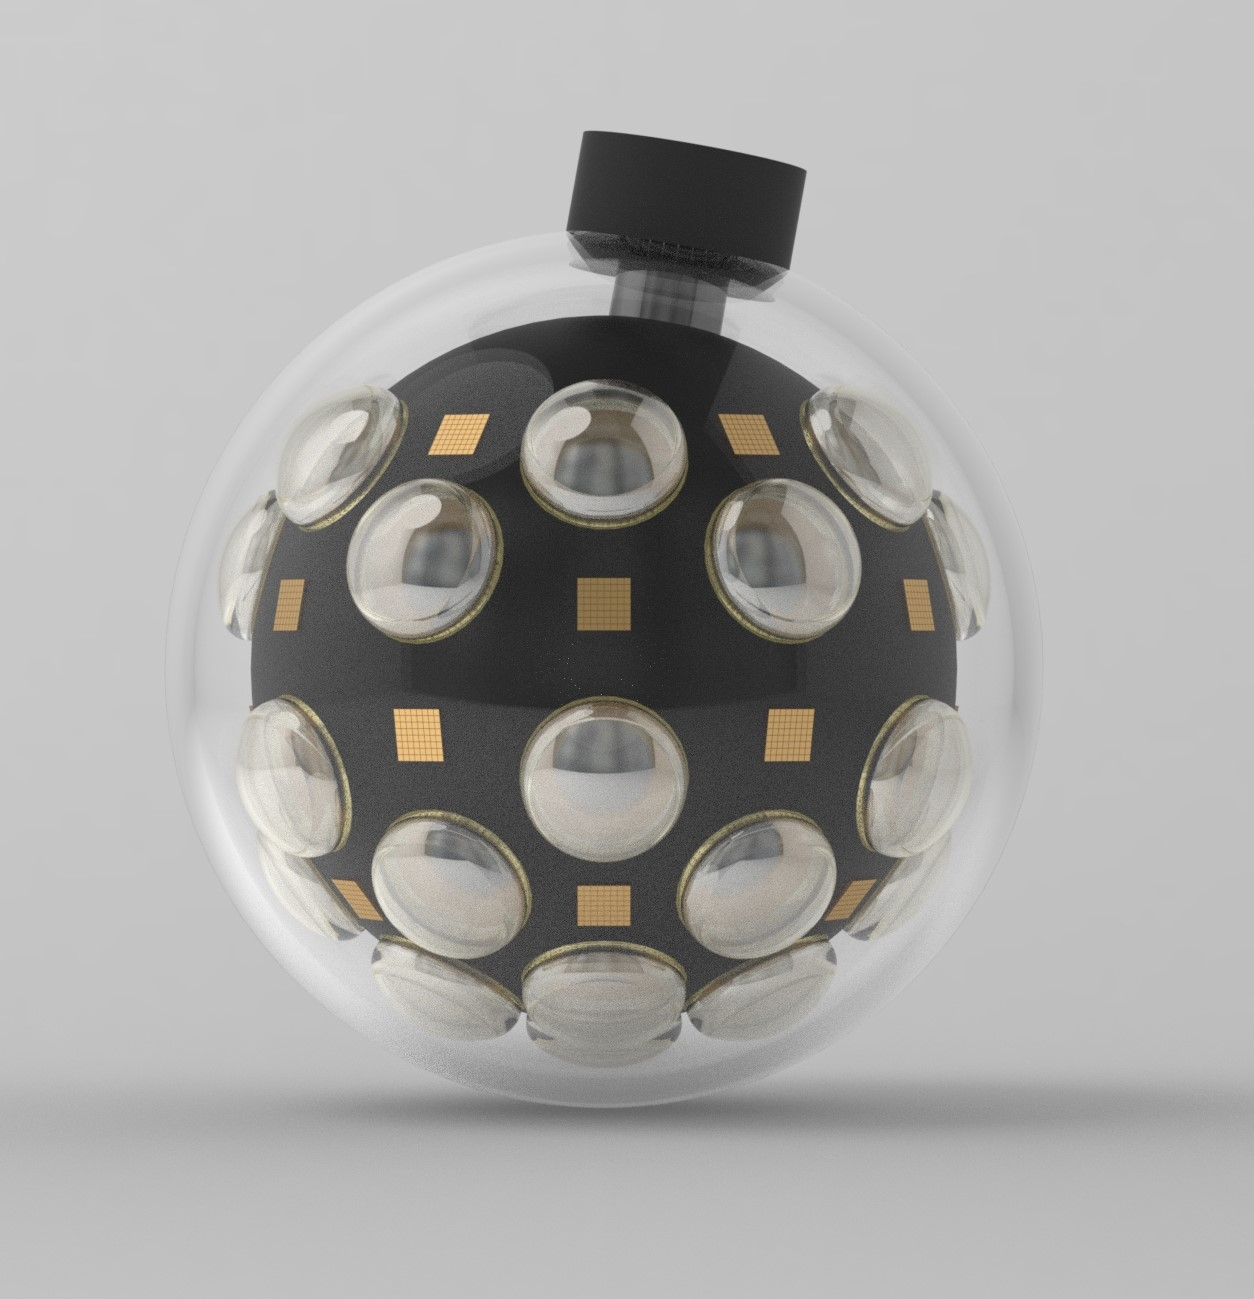
\includegraphics[width=0.7\textwidth]{img/hDOM_rendering.jpg}
    \caption{目前设计的hDOM内部结构的渲染图。}
    \label{fig:hDOM_rendering}
\end{figure}


海铃中微子望远镜的探测单元——hDOM(hybrid Digital Optical Module)的内部结构比较复杂,它包含有PMT和SiPM两种不同的光敏元件。
目前有关PMT和SiPM在探测器内部的几何布局仍然处于积极的研究中,我们需要通过模拟来对比不同排列下的探测器的光子接收面积。
此外,PMT周围的反射环或者光学胶等辅助结构也同样会影响最终PMT的探测效率\cite{IceCube-Gen2_gel_pad:2021}。
因此对于光子在hDOM内部的传播过程的模拟需要一个物理上准确并且可控程度高的程序来处理,在海铃的模拟框架中,我们基于Geant4构建了一个专门的模拟程序\footnote{\url{https://gitlab.com/hailing/hdom}}。
Geant4中存在完整的光子在介质中的吸收和散射,以及光子在穿越不同折射率的介质界面时发生的透射和反射过程。
此外Geant4中还可以通过将几个不同的基本几何体进行交集,并集和补集的操作来构建出复杂而且精细的几何,从而满足未来对探测器内部精细设计的需求。
因此Geant4非常适合对光敏探测元件进行精细的模拟。

我们可以在该程序中构建精细的hDOM内部几何结构,其目前的设计版本所对应的渲染图如\ref{fig:hDOM_rendering}所示。
在当前的设计中,hDOM的最外层是一个17英寸硅硼酸玻璃球壳\footnote{\url{https://www.vitrovex.com/instrument_spheres}},
其外径$21.6\,\mathrm{cm}$,内径$20.2\,\mathrm{cm}$,
密度为$3.0\,\mathrm{g/cm^3}$,折射率为$1.47$。
玻璃球壳内为一个半径为$16.4\,\mathrm{cm}$的不透光的3D打印支架。PMT和SiPM嵌在在3D支架外围。
玻璃球壳和3D支架中间填充着高透明度的光学胶\footnote{\url{https://www.wacker.com/h/en-us/silicone-rubber/silicone-gels/wacker-silgel-612-ab/p/000007546}},其密度为$0.97\,\mathrm{g/cm^3}$,折射率为$1.40$。
光学胶的折射率与外层硅硼酸玻璃以及内部的PMT的玻璃外壳的折射率接近,可以减少光子的界面损失。
在3D打印的支架上安插着31支直径为$3\,\mathrm{inch}$的PMT和24个边长为$\sim 3\,\mathrm{cm}$的SiPM阵列。
这些PMT和SiPM被包裹在凝固之后的光学胶之中,是最终接收探测光子的光敏元件。

在上一步的海水介质的光传播模拟中,光子在hDOM表面的波长和方向信息被记录下来。
这些光子会在hDOM模拟程序中重新发射,光子从hDOM的玻璃球壳外表面处向内传播,如果能够被PMT或者SiPM这样的光敏元件接收,则将其记录下来,作为最终探测器接收到的击中信息。

\subsection{光敏元件响应模拟}

\begin{figure}[htb]
\centering
    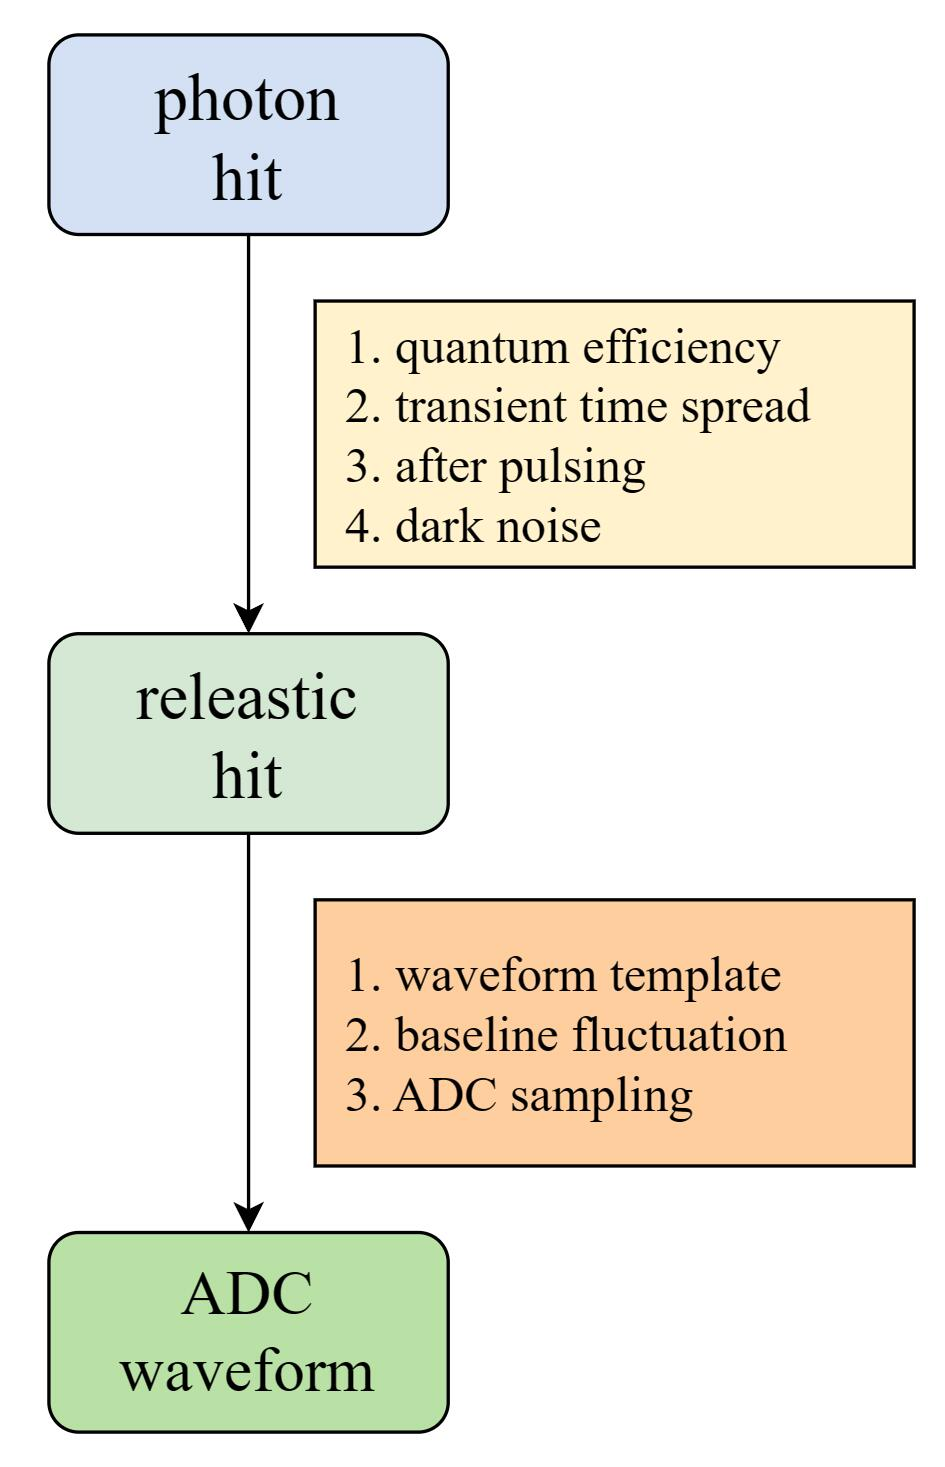
\includegraphics[width=0.5\textwidth]{img/waveform_simulation.jpg}
    \caption{波形模拟程序中的数据流程图。}
    \label{fig:waveform_simulation}
\end{figure}

击中PMT表面的光子,将会经过PMT信号放大成可观测的电信号,随后由模数转换器(Analog Digital Converter,ADC)转换为时间上的电压序列,即波形信号。
我们构建了一个可以模拟PMT对光子的响应的PMT波形模拟程序\footnote{\url{https://gitlab.com/hailing/hailing-wf-simulator}},它可以模拟从光子击中PMT的光阴极到PMT的阳极中输出波形信号以及最终被读数电路放大并数字化的过程,其程序中的数据流如图\ref{fig:waveform_simulation}中所示。

目前该程序的功能框架已经完备,但具体PMT的详细物理性能还有待测试,电子学读数电路尚未制作完成,其性能要求也仍在评估中。

从理论上来说,SiPM对光子的响应波形与PMT类似,具体而言SiPM会拥有更好的时间分辨能力,量子效率以及单光子分辨率,但同时也会有更严重的暗噪声和串扰现象。
由于我们实验团队对SiPM自身的硬件性能测试还处于早期阶段,因此对模拟SiPM响应的模拟程序暂未开发。

    \chapter{中微子望远镜性能分析}
\label{chap:telescope_performance}

在本章节中,我们研究我们的切伦科夫中微子望远镜对缪子中微子产生的径迹型事件的响应性能。
在模拟和分析研究中,我们以章节\ref{sec:TRIDENT_array}中所介绍的海铃阵列的配置为标准。

\section{角度分辨率}
\label{sec:angular_resolution}

IceCube观测到的弥散中微子流量已经对天体中微子源的参数空间产生了极大的限制:这些源的数量密度必须足够大,而单个源的流强非常微弱。
为了从弥散中微子流量中挖掘出这些微弱的中微子源,下一代的中微子望远镜必须拥有更强的角分辨率\cite{Fang_resolve_flux:2016}。
在本小节中,我们对模拟出来的径迹型中微子事件进行方向重建,通过观察重建的误差来判断海铃的角度分辨率。

中微子望远镜中DOM的大小和分布密度相对于其监控的广袤的海水而言是极其稀疏的。
在一次中微子事件中,大约只有$10^{-7}$的光子信息能够被望远镜中的光敏元件所捕获。
因此,中微子望远镜不是一个量能器,它并不能将粒子所有的能量都沉积其中并且全部测量,相反的,中微子望远镜是一种典型的稀疏采样探测器。
中微子望远镜的重建过程,便是要通过这些有限的光子信息来推断出中微子的动力学信息,即能量,位置和运动方向。

\begin{figure}[!htb]%
    \centering
    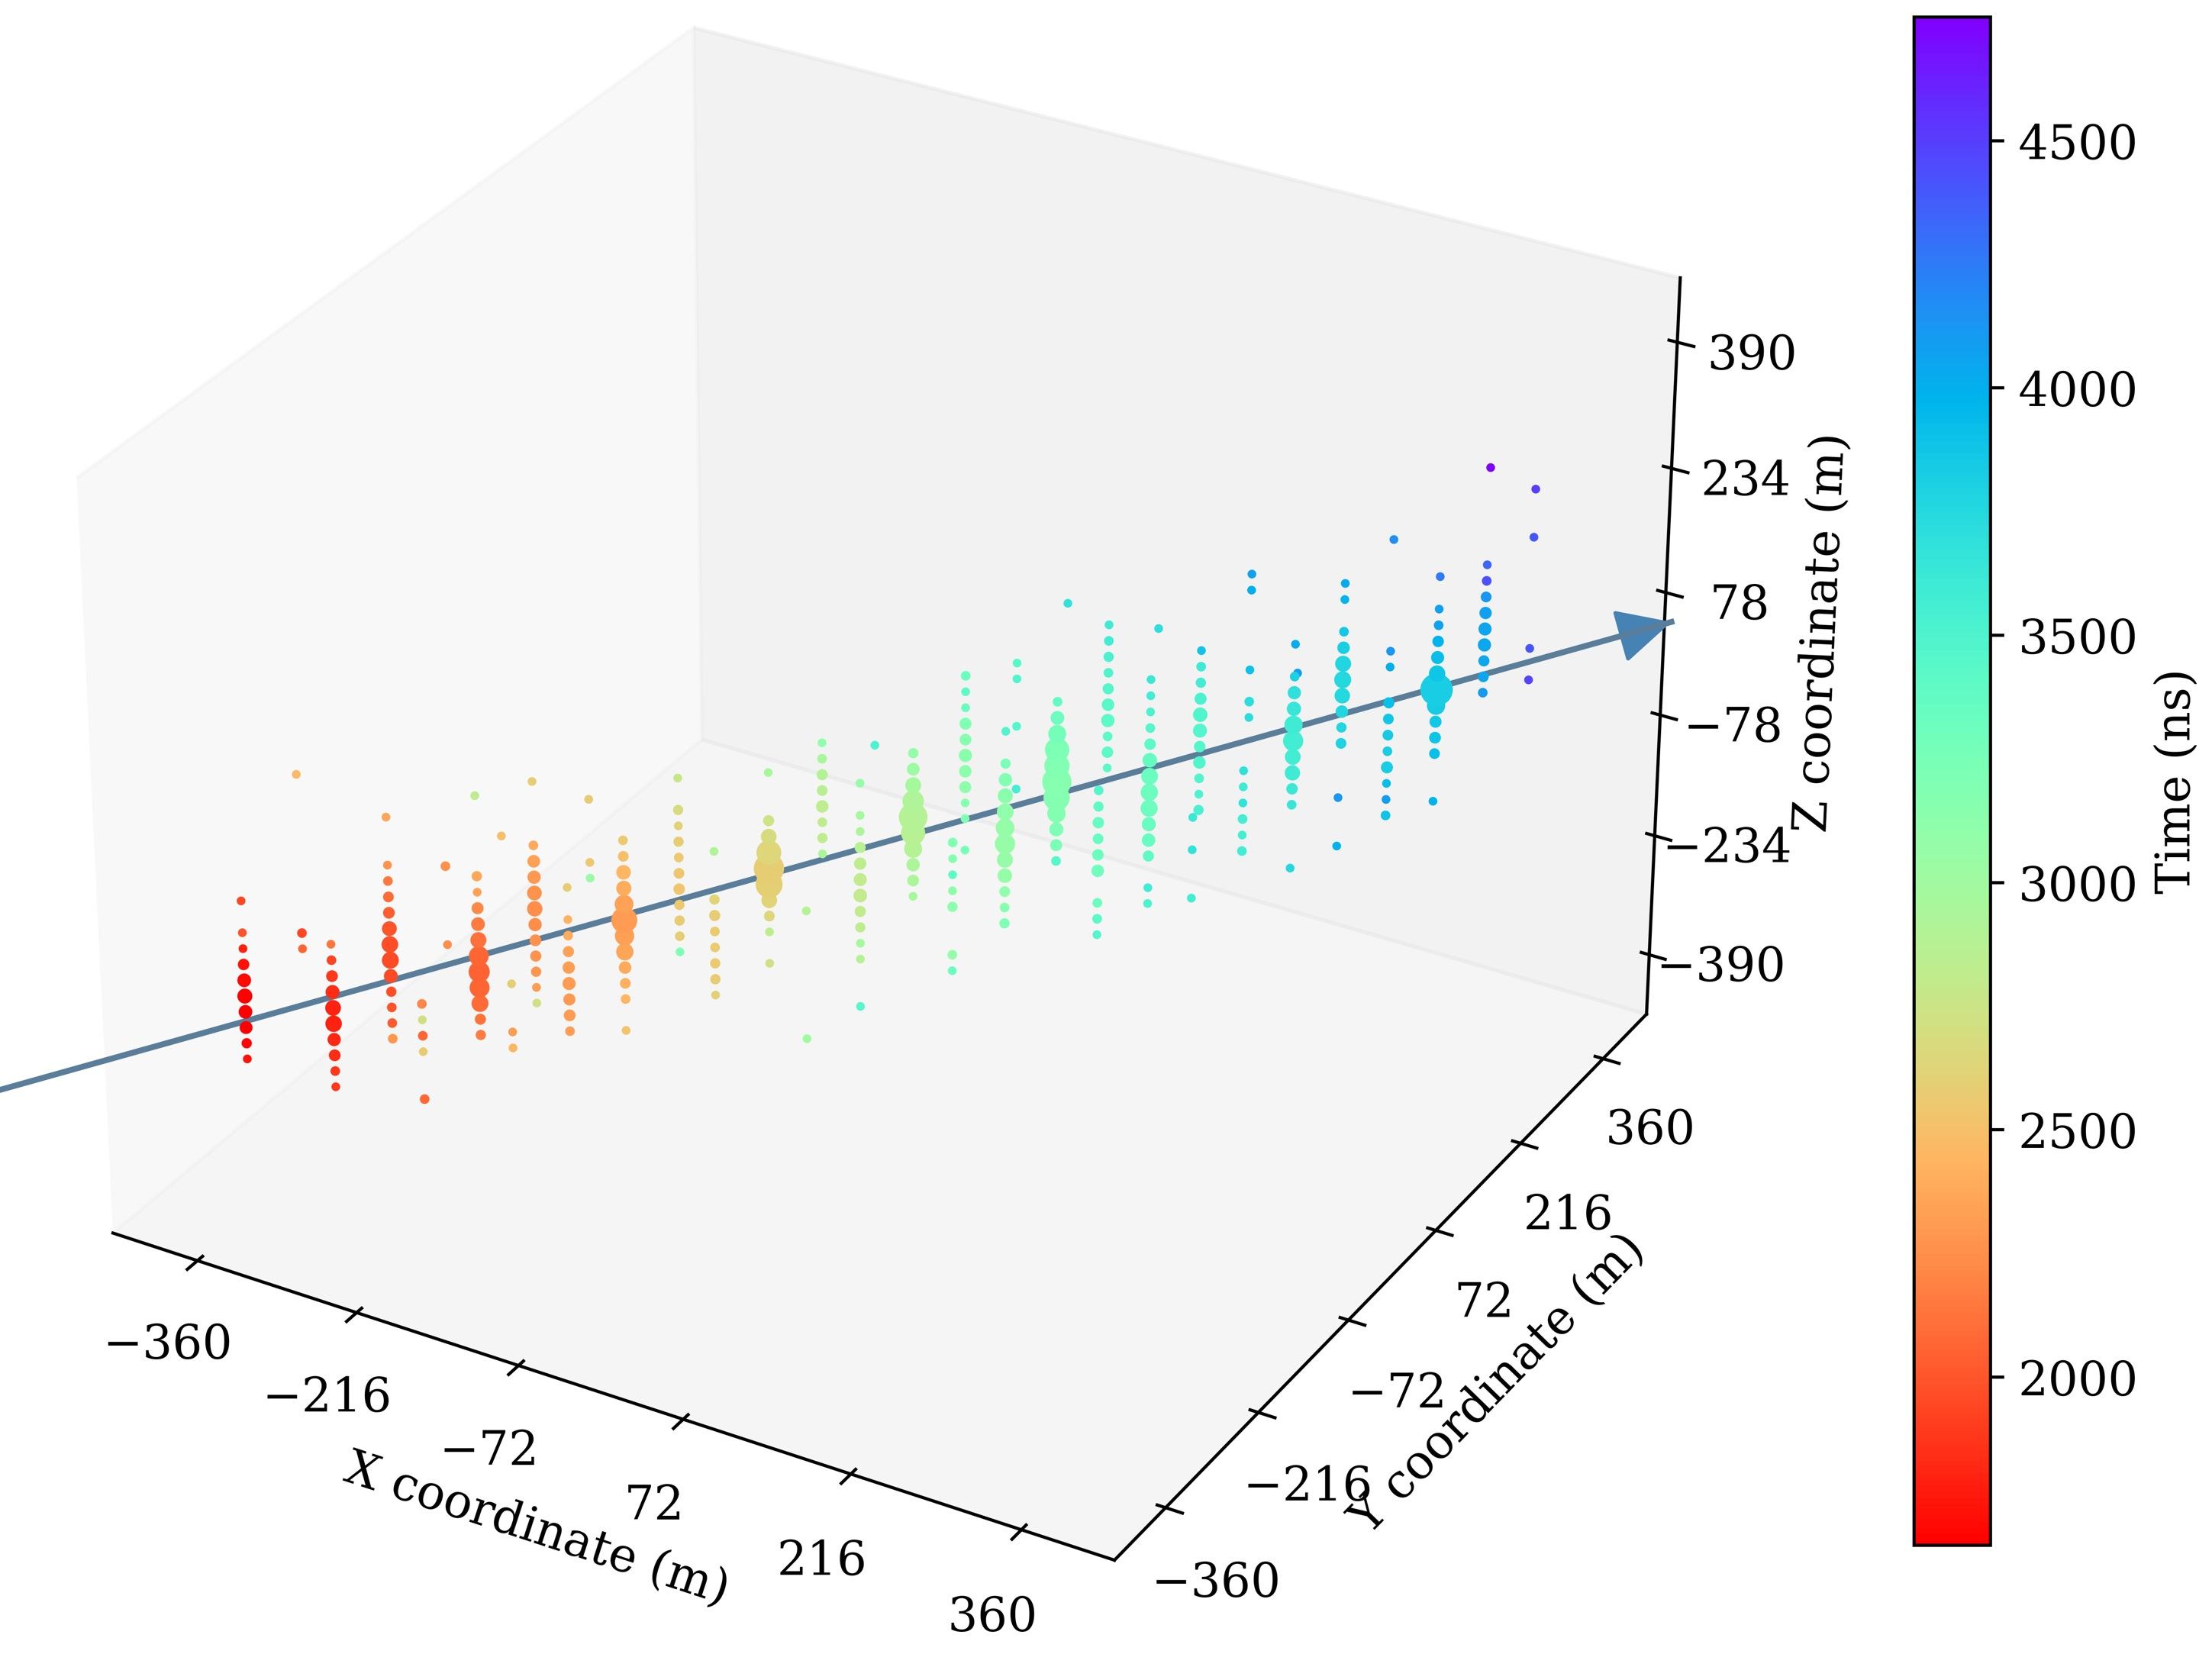
\includegraphics[width=0.75\textwidth]{img/track-like_event.jpg}
    \caption{一个$10\,\mathrm{TeV}$能级的缪子在中微子望远镜中的轨迹。图中的每一个圆点都表示一个接收到光子的hDOM,圆点的大小表示接收到的光子的数量,颜色表示光子到达hDOM的时间。}
    \label{fig:track-like_event}
\end{figure}

一个典型的由缪子产生的径迹型事件在中微子望远镜中留下的轨迹如图\ref{fig:track-like_event}中所示。
从图中我们可以看到,通过阵列中的hDOM的位置与其接收到的光子的时间信息,我们可以看出缪子在阵列中的穿行轨迹。根据这些信息,我们可以对缪子事件进行重建。

\subsection{初步拟合}
\label{subsec:track_reco_first_guess}

对中微子事件的初步拟合是为了针对那些比较低层次,质量杂乱的大量中微子事件,它能够快速确定一个大致的事件方向,也可以用于估计一个事件质量\cite{line_fit:2013, ANTARES_q_fit:2011}。此外,初步拟合得到的方向结果可以作为后续精细拟合的输入参数。

\begin{figure}[!htb]%
    \centering
    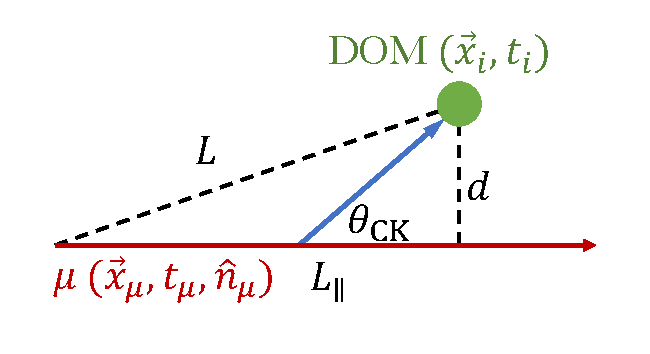
\includegraphics[width=0.75\textwidth]{img/Cherenkov_geometry_DOM_observation.pdf}
    \caption{缪子径迹发射出切伦科夫光子,击中到hDOM上的示意图。}
    \label{fig:Cherenkov_geometry_DOM_observation}
\end{figure}

如图\ref{fig:Cherenkov_geometry_DOM_observation}中所示,假设每一个被光子击中的hDOM的位置和击中时间分别为$\vec{x}_i$和$t_i$,缪子径迹的初始位置,时间和方向分别为$\vec{x}_\mu$,$t_\mu$和$\hat{n}_\mu$。
在初步拟合中,我们首先将缪子产生的切伦科夫光简单地近似成一束与缪子方向平行的平面光,此时hDOM接收的击中信息与初始缪子的运动状态之间应当有如下的近似关系:
\begin{equation}
    t_i \simeq (\vec{x}_i - \vec{x}_\mu) \cdot \hat{n}_\mu + t_\mu ,
\end{equation}
通过对上式进行最小二乘法拟合,我们可以得到对缪子运动信息的初步分析结果。

有了如上的初步结果之后,我们进一步地对缪子的状态进行最大似然估计,在估计中我们所采用的主要观测量为hDOM测量到的光子到达时间的残差$t_i^\mathrm{res}$\cite{AMANDA_track_reco:2003},其定义如下:
\begin{equation}
    t_i^\mathrm{res}(\vec{x}_\mu, t_\mu, \hat{n}_\mu) = t_i - t_i^\mathrm{geo}(\vec{x}_\mu, t_\mu, \hat{n}_\mu),
\end{equation}
其中$t_i^\mathrm{geo}(\vec{x}_\mu, t_\mu, \hat{n}_\mu)$表示在某一径迹假设下,光子到达的几何时间,即切伦科夫光锥面到达该位置的hDOM的时间,根据图\ref{fig:Cherenkov_geometry_DOM_observation}中所示,我们可以写下$t_i^\mathrm{geo}$的表达式:
\begin{equation}
\begin{aligned}
    t_i^\mathrm{geo} &= t_\mu + (L_\parallel - \frac{d}{\tan(\theta_\mathrm{CK})}) / c + \frac{d}{\sin(\theta_\mathrm{CK})} / \frac{c}{n_\mathrm{g}} \\
    &= t_\mu + \frac{L_\parallel}{c} + \frac{d}{c} \times 
    \frac{n_\mathrm{g} n_\mathrm{p} - 1}{\sqrt{n_\mathrm{p}^2 - 1}} \\
    L = \lvert &\vec{x}_i - \vec{x}_\mu \rvert, ~~
    L_\parallel = \lvert (\vec{x}_i - \vec{x}_\mu) \cdot \hat{n}_\mu \rvert, ~~ d = \sqrt{L^2 - L_\parallel^2}
    \label{eq:t_geo}
\end{aligned}
\end{equation}
需要注意的是,介质中的散射效应会导致光子并非沿着直线直接到达hDOM,因此光子的真实到达$t_i$可能会晚于$t_i^\mathrm{geo}$。此外,介质的色散效应以及光敏探测元件自身的时间分辨率会导致观测到的$t_i$也出现一定的弥散。

在处理到达时间时,对于每一个hDOM,我们都只选择出其接收到的第一个光子的到达时间$t_i^\mathrm{1st}$而忽略其余剩下的光子的到达时间,这是因为第一个到达的光子更有可能是没有经过任何散射而直接到达hDOM的。
并且考虑到SiPM的时间分辨性能要高于PMT,在一个hDOM中的PMT和SiPM都同时有信号的情况下,我们优先采用SiPM中测量到的时间。

我们首先构建一个形式上最为简洁,并且计算效率和稳定性都非常良好的最大似然函数$\mathcal{L}^M$,我们称之为M-estimator:
\begin{equation}
    \ln \mathcal{L}^M(\vec{x}_\mu, t_\mu, \hat{n}_\mu; \vec{x}_i, t_i^\mathrm{1st}) = 
    \sum_i \left(2 - 2 \sqrt{ (t_i^\mathrm{res})^2/2 + 1 } \right) .
\end{equation}
这样构造出来的似然函数在数学上是一个凸函数,因此能够很快得收敛到全局最优解。
然而$\mathcal{L}^M$中的$t_i^\mathrm{res}$的概率分布函数并非是真正物理上的分布函数。

\subsection{光子到达时间分布函数}

由于光子的行为在经过多次散射之后就变得难以估计,因此我们依赖于使用数值模拟的方法,从大量的模拟得到的$t^\mathrm{res}$中去估计出它的分布函数。
我们模拟得到的$t^\mathrm{res}$如图\ref{fig:residual_time_distribution}中所示。
我们将$t^\mathrm{res}$表示为一个与hDOM的位置到径迹的距离$d$相关的函数$t^\mathrm{res}(d)$,这是考虑到它们之间的距离决定了光子从发射到被接收时中间走过的距离,而这正决定了光子经历的散射次数。

为拟合模拟中得到的分布,我们采用了如下形式的函数来表示$t^\mathrm{res}$的分布:
\begin{equation}
    p(\tau) = \frac{1}{\pi (\tau^2+1)} \times \frac{2}{e^{-\alpha \tau} + 1} ,
    \label{eq:residual_time_PDF}
\end{equation}
其中,$\tau = (t_\mathrm{res} - \mu) / \sigma$是经过平移并且无量纲化之后的到达时间残差,$\alpha$表示分布的倾斜程度。
式\ref{eq:residual_time_PDF}中的第一项表示一个柯西分布,它被用于描述到达时间的不确定性;而第二项是一个sigmoid函数,它使得原本沿着$y$轴对称的柯西分布向右侧倾斜,从而可以表示散射光子到达时间的延后。
式\ref{eq:residual_time_PDF}很好地展现出在海水中,大部分的光子都可以直接到达探测器,进而在$t_\mathrm{res} = 0\,\mathrm{ns}$的位置形成一个峰,而少部分光子则会延后到达。
此外,相比于过去其他实验所使用的伽马分布\cite{AMANDA_track_reco:2003},公式\ref{eq:residual_time_PDF}在$t_\mathrm{res} < 0$的区域也是良好定义的,可以表现出由于光子色散和探测器的事件响应精度问题而导致光子先于几何时间到达探测器,并且在数值求解的过程中也有较好的稳定性。

我们将公式中的形状参数$\mu$,$\sigma$和$\alpha$表示为有关hDOM到径迹的距离$d$的一次函数,对模拟得到的数据点进行拟合,其得到的结果如下:
\begin{equation}
    \mu = 0.0199 d - 0.114,~~
    \sigma = 0.0669 d + 0.328,~~
    \alpha = 0.0127 d + 0.538 ,
    \label{eq:residual_time_parameters}
\end{equation}
我们在拟合的过程中只采用了光子到达时间位于2.5\%到70.5\%之间的数据,因为这部分光子是最有可能成为第一个到达的光子。拟合结果与实验模拟数据之间的比较如图\ref{fig:residual_time_distribution}中所示。

\begin{figure}[!htb]%
    \centering
    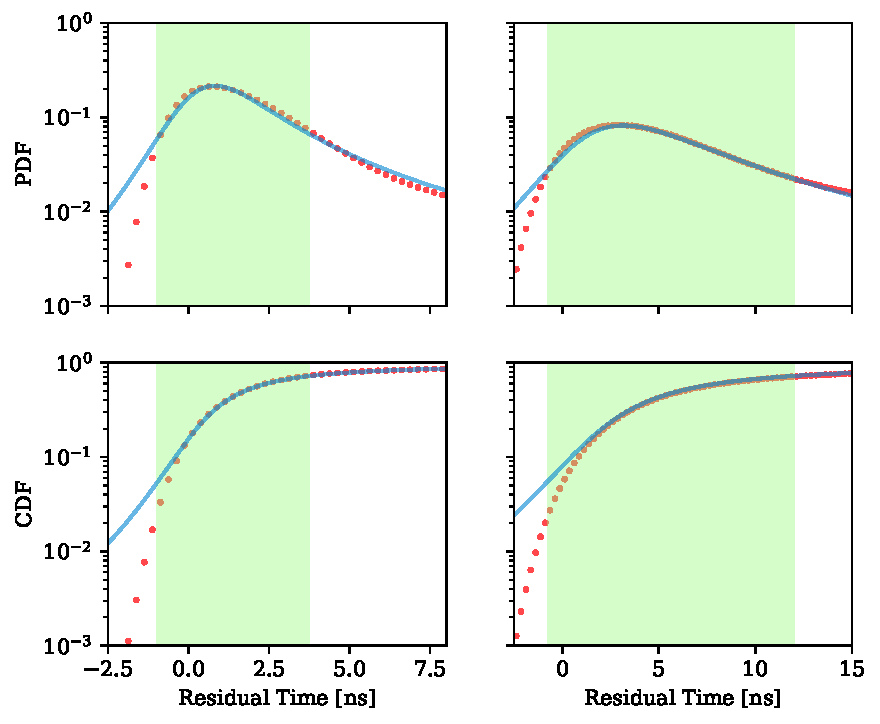
\includegraphics[width=0.85\textwidth]{img/residual_time_distribution.pdf}
    \caption{模拟得到的光子到达时间残差$t^\mathrm{res}$的分布以及解析拟合。左图为hDOM到径迹距离$d = 20 \,\mathrm{m}$下的分布,右图为$d = 70 \,\mathrm{m}$下的分布。上图为概率密度分布函数,而下图为累积分布函数。图中绿色的阴影区域表示累积分布函数的值为2.5\%和70.5\%的区域范围,只有在这个范围内的概率分布函数数据点才被用于拟合解析表达式。}
    \label{fig:residual_time_distribution}
\end{figure}

有了更为准确的光子到达时间表示之后,我们可以将构造更为精细的似然函数:
\begin{equation}
    \mathcal{L}(\vec{x}_\mu, t_\mu, \hat{n}_\mu; \vec{x}_i, t_i^\mathrm{1st}) = 
    \prod_i \left( \frac{1}{\pi (\tau^2+1)} \times \frac{2}{e^{-\alpha \tau} + 1} \right),
    \label{eq:track_reco_likelihood}
\end{equation}
将上一节中的初步重建结果作为初始条件代入到优化算法中,我们可以寻找使得\ref{eq:track_reco_likelihood}达到最大值的径迹方向。


\subsection{重建结果}

对不同入射能量缪子中微子产生的径迹型事件,我们的重建结果如图\ref{fig:angular_resolsution}中所示。
我们可以看到我们的重建算法对能量仅为$1\,\mathrm{TeV}$的中微子事件也可以达到$\sim 0.3^\circ$的重建精度,但此时中微子和缪子在反应顶点处的本征方向误差占据主导地位,因此望远镜对真实中微子的角分辨率处于$\lesssim 1^\circ$的水平。
而在$100\,\mathrm{TeV}$到$1\,\mathrm{PeV}$的能量范围内,探测器的角分辨率可以达到$\sim 0.1^\circ$的量级,达到了世界最顶尖的角分辨率水平。
如此优越的性能与探测器中采用的SiPM光敏元件的高时间分辨率有直接的关系,有关此内容的讨论参见章节\ref{sec:hdom}。


\begin{figure}[!htb]%
    \centering
    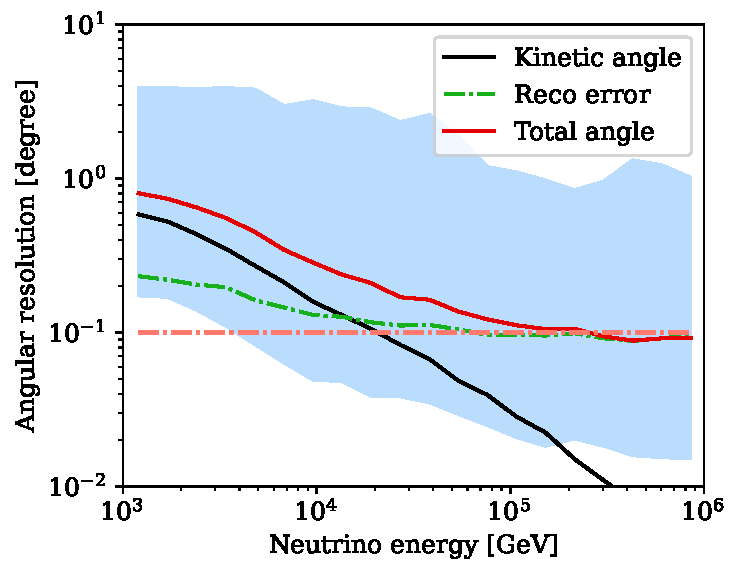
\includegraphics[width=0.75\textwidth]{img/angular_resolsution.pdf}
    \caption{对不同的缪子中微子产生的径迹型事件进行重建后,得到的中微子望远镜的角分辨率。图中绿色点虚线表示对缪子径迹的重建误差,黑色实线表示中微子与DIS反应得到的缪子之间的动能夹角,红色实线表示重建得到的径迹方向与真实中微子方向之间的误差,这三条线均表示角度误差的中位数。蓝色阴影带状区域表示重建得到的径迹方向与真实中微子方向之间的误差的$1\sigma$分布区域。}
    \label{fig:angular_resolsution}
\end{figure}



\section{有效面积}

在本节中,我们研究海铃中微子望远镜对缪子径迹型事件的有效面积。探测器的有效面积$A_\mathrm{eff}$是衡量探测器能够探测到的事例率的重要性能指标。
假设中微子的物理流量为$F_\mathrm{phy}(\hat{n}, E)$,探测器的有效面积被定义为:
\begin{equation}
    A_\mathrm{eff} (\hat{n}, E) \equiv \frac{\mathrm{d}N}{\mathrm{d}t \,\mathrm{d}\Omega \,\mathrm{d}E} (\hat{n}, E) / 
    F_\mathrm{phy}(\hat{n}, E) ,
    \label{eq:eff_area_init}
\end{equation}
其中$\frac{\mathrm{d}N}{\mathrm{d}t \,\mathrm{d}\Omega \,\mathrm{d}E}(E, \hat{n})$表示在某一能量$E$和方向$\hat{n}$上,单位时间单位能量单位立体角上,探测器所能观测到的事件数量。

在后面的分析计算中,我们将会看到探测器的有效面积与具体的中微子辐射源无关,其反应的是探测器的本质性能。
尽管如此,我们通常借助于一些假定的中微子源,通过蒙特卡洛采样的方法研究探测器对不同中微子事件的响应,进而分析出探测器的有效面积。


\subsection{采样权重}
\label{subsec:weightings}

考虑真实的物理情况,对于任意的中微子流强$F_\mathrm{phy}(E, \hat{n})$而言,在单位能量单位时间单位空间单位立体角内,中微子在某一个点上发生DIS过程的数量是:
\begin{equation}
\begin{aligned}
    \frac{\mathrm{d}N}{\mathrm{d}E ~\mathrm{d}\Omega ~\mathrm{d}t ~\mathrm{d}V} (E, \hat{n}, \vec{x})
    &= F_\mathrm{phy}^\mathrm{surv} (\hat{n}, E, X)\times \frac{1}{\lambda_\mathrm{int}(E)} \\
    &= F_\mathrm{phy}(\hat{n}, E) \times P_\mathrm{surv}(E, X) \times \frac{1}{\lambda_\mathrm{int}(E)} , \\
    P_\mathrm{surv}(E, X) = e&^{- \frac{\sigma_\mathrm{tot}(E) \times X(\hat{n}, \vec{x})}{m_{p}}}, ~~~
    X(\hat{n}, \vec{x}) = \int_l \rho(\vec{x'}) \,\mathrm{d}\vec{x'}, ~~~
    \lambda_\mathrm{int}(E) = \frac{m_{p}}{\rho(\vec{x}) \sigma_\mathrm{DIS}(E)}
\end{aligned}
\label{eq:sampling_phy_pdf}
\end{equation}
其中$E$,$\hat{n}$和$\vec{x}$分别表示中微子的能量,方向和位置。
$F_\mathrm{phy}^\mathrm{surv} (\hat{n}, E, X)$表示在地球中穿过柱密度$X$之后,能够存活下来的中微子的流强。
$P_\mathrm{surv}(E, X)$表示存活概率,$\sigma_\mathrm{tot}(E)$表示中微子与物质相互作用的总散射截面,柱密度$X(\hat{n}, \vec{x})$与中微子在地球中的路径以及地球的密度模型有关。
$\lambda_\mathrm{int}(E)$表示中微子的反应自由程,$m_p$表示质子质量\footnote{这里我们忽略了质子与中子之间散射截面与质量的差异,而用同位旋为0的核子来表示散射截面,用$m_p$来表示质子和中子的平均质量。}
$\rho(\vec{x})$表示介质的密度,与地球的密度模型有关,$\sigma_\mathrm{DIS}(E)$表示感兴趣的DIS反应通道的散射截面。

以一个具体的问题为例,假设我们要研究探测器能探测到的中微子事例率,那么我们可以通过如下表达式来计算实例率:
\begin{equation}
    \frac{\mathrm{d}N}{\mathrm{d}t} = 
    \int \mathrm{I}_\mathrm{sel}(s) \times \frac{\mathrm{d}N}{\mathrm{d}E ~\mathrm{d}\Omega ~\mathrm{d}t ~\mathrm{d}V} 
    ~\mathrm{d}E ~\mathrm{d}\hat{n} ~\mathrm{d}\vec{x} ,
    \label{eq:sampling_phy_trigger}
\end{equation}
其中我们引入了符号$s$(signal)来表示由能量$E$,方向$\hat{n}$的中微子在位置$\vec{x}$发生DIS过程引起的探测器探测到的信号。严格来说$s$是一个分布,因为粒子的相互作用结果是不确定的,同样的中微子所引发的事件会产生不同的信号,这种不确定性可以通过大量的模拟采样来消除。
$\mathrm{I}_\mathrm{sel}(s)$表示事件筛选算法对事件$s$的响应结果,它根据信号的强弱程度,质量高低,以及与分析目标的符合程度返还1或者0的值。

在我们的重要性采样的过程中,我们使用蒙特卡洛采样的方式来代替积分,即我们将积分运算理解为了对物理量求期望。
蒙特卡洛采样中注入的模拟事件在相空间中的具体分布是可以由我们自己设计的,通常我们会将之与感兴趣的物理研究对象联系在一起,例如侧重于某一中微子的能量和入射角区间。
假如我们采用了如下的能量,方向和位置的分布函数:
\begin{equation}
    P_\mathrm{mc} (E, \hat{n}, \vec{x}) = F_\mathrm{mc} (E, \hat{n}) \times n_\mathrm{mc}(\vec{x}) ,
    \label{eq:sampling_MC_pdf}
\end{equation}
其中$F_\mathrm{mc} (E, \hat{n})$是我们想要研究并且在模拟中注入的中微子能谱,有$E^{-1} \Omega^{-1}$的量纲,$n_\mathrm{mc}(\vec{x})$是注入的中微子反应事件的顶点在空间上的分布函数,有$V^{-1}$的量纲。
在真实物理世界中,中微子流强的能谱指数$\alpha_\mathrm{phy}$通常为$-2$到$-3$,在这种情况下,探测器探测到的信号绝大多数都是低能的无法通过质量筛选的信号,对这些低能信号做模拟将会浪费大量的计算资源。
而在重要性采样中,我们可以将能谱指数$\alpha_\mathrm{mc}$设计成$-1$到$-1.5$,以此来产生更多的我们感兴趣高能的事件。

我们将我们的蒙特卡洛采样的分布函数插入到式\ref{eq:sampling_phy_trigger}中,可以得到:
\begin{equation}
\begin{aligned}
    \frac{\mathrm{d}N}{\mathrm{d}t} &= 
    \int \mathrm{I}_\mathrm{sel}(s) \times 
    \frac{\mathrm{d}N}{\mathrm{d}E ~\mathrm{d}\Omega ~\mathrm{d}t ~\mathrm{d}V}(E, \hat{n}, \vec{x}) 
    ~\mathrm{d}E ~\mathrm{d}\hat{n} ~\mathrm{d}\vec{x} \\
    &= \int \mathrm{I}_\mathrm{sel}(s) \times 
    \frac{\mathrm{d}N}{\mathrm{d}E ~\mathrm{d}\Omega ~\mathrm{d}t ~\mathrm{d}V} (E, \hat{n}, \vec{x})
    \times \frac{1}{P_\mathrm{mc} (E, \hat{n}, \vec{x})} \times P_\mathrm{mc} (E, \hat{n}, \vec{x})
    ~\mathrm{d}E ~\mathrm{d}\hat{n} ~\mathrm{d}\vec{x} \\
    &= \mathbb{E}_s \left[ \mathrm{I}_\mathrm{sel}(s) \times 
    \frac{\mathrm{d}N}{\mathrm{d}E ~\mathrm{d}\Omega ~\mathrm{d}t ~\mathrm{d}V} (E, \hat{n}, \vec{x})
    \times \frac{1}{F_\mathrm{mc} (E, \hat{n}) \times n_\mathrm{mc}(\vec{x})}   \right]  \\
    &= \frac{1}{N_\mathrm{tot}} \sum^N_i \left[ 
    \mathrm{I}_\mathrm{sel}(s_i) \times 
    \frac{\mathrm{d}N}{\mathrm{d}E ~\mathrm{d}\Omega ~\mathrm{d}t ~\mathrm{d}V} (E_i, \hat{n}_i, \vec{x}_i)
    \times \frac{1}{F_\mathrm{mc} (E_i, \hat{n}_i) \times n_\mathrm{mc}(\vec{x}_i)} \right]
\end{aligned}
\label{eq:sampling_MC_trigger}
\end{equation}
在最后一步中,我们用蒙特卡洛采样的方式代替了期望计算。其中$s_i$表示某一个根据$P_\mathrm{mc} (E, \hat{n}, \vec{x})$分布采样得到的模拟事件样本,$N_\mathrm{tot}$表示采样样本总数。

进一步的,我们将中微子发生反应的表达式(\ref{eq:sampling_phy_pdf})带入到事例率的表达式(\ref{eq:sampling_MC_trigger})中,并且将结果拆解成更加模块化的组分:
\begin{equation}
\begin{aligned}
    \frac{\mathrm{d}N}{\mathrm{d}t} 
    &= \frac{1}{N_\mathrm{tot}} \sum^N_i \left[ \mathrm{I}_\mathrm{sel}(s_i) \times 
    \frac{\mathrm{d}N}{\mathrm{d}E ~\mathrm{d}\Omega ~\mathrm{d}t ~\mathrm{d}V} (E_i, \hat{n}_i, \vec{x}_i)
    \times \frac{1}{F_\mathrm{mc} (E_i, \hat{n}_i) \times n_\mathrm{mc}(\vec{x}_i)} \right] \\
    &= \frac{1}{N_\mathrm{tot}} \sum^N_i \left[ \mathrm{I}_\mathrm{sel}(s_i) \times 
    F_\mathrm{phy}(E_i, \hat{n}_i) \times
    P_\mathrm{surv}(E_i, X_i) \times
    \frac{1}{\lambda_\mathrm{int}(E_i)} \times
    \frac{1}{F_\mathrm{mc} (E_i, \hat{n}_i)} \times
    \frac{1}{n_\mathrm{mc}(\vec{x}_i)} \right]
\end{aligned}
\label{eq:sampling_MC_terms_trigger}
\end{equation}

在上述表达式中,$\mathrm{I}_\mathrm{sel}(s)$依赖于探测器的探测能力以及对事件的筛选方式,中微子的物理流量$F_\mathrm{phy}(E, \hat{n})$对应于具体的某一个中微子源的测量结果或者对源流量的假设,$\lambda_\mathrm{int}(E)$与$P_\mathrm{surv}(E, X)$与中微子与物质的散射截面以及地球模型相关,$F_\mathrm{mc} (E, \hat{n})$和$n_\mathrm{mc}(\vec{x})$与采样的方式有关。在实际应用中,我们将后面四项作为权重项:
\begin{equation}
\begin{aligned}
    w_\mathrm{tot} &= w_\mathrm{surv} \times w_\mathrm{int} \times w_\mathrm{flux} \times w_\mathrm{vol} \\
    w_\mathrm{surv} &= P_\mathrm{surv}(E, X), &\mathrm{dim}(1) \\
    w_\mathrm{int} &= \frac{1}{\lambda_\mathrm{int}(E)}, &\mathrm{dim}(L^{-1}) \\
    w_\mathrm{flux} &= \frac{1}{F_\mathrm{mc}(E, \hat{n})},  &\mathrm{dim}(E \Omega) \\
    w_\mathrm{vol} &= \frac{1}{n_\mathrm{mc}(x_i)} = V_\mathrm{sample}, &\mathrm{dim}(L^{3}) ,\\
\end{aligned}
\label{eq:weighting_terms}
\end{equation}
其中$w_\mathrm{tot}$表示总的权重大小。将其带回式子\ref{eq:sampling_MC_terms_trigger}中可以得到:
\begin{equation}
    \frac{\mathrm{d}N}{\mathrm{d}t} = 
    \frac{1}{N_\mathrm{tot}} \sum^N_i \left[ 
    \mathrm{I}_\mathrm{sel}(s_i) \times 
    F_\mathrm{phy} (E_i, \hat{n}_i) \times
    w_{\mathrm{tot}, i} \right]
\label{eq:sampling_trigger_rate}
\end{equation}

公式\ref{eq:weighting_terms}中的$V_\mathrm{sample}$表示采样的体积,在章节\ref{subsec:muon_sampling}中所描述的针对径迹型缪子中微子事件的采样模式下,我们的采样体积为:
\begin{equation}
    V_\mathrm{sample}^\mathrm{track} = \pi R_0^2 (D_\mu + 2D_0) ,
    \label{eq:weighting_volume}
\end{equation}
而对于普通的非径迹型中微子事件,只有当DIS反应的顶点位置发生在望远镜阵列的内部时,事件才可以被探测到,因此采样体积即为探测器的几何体积:
\begin{equation}
    V_\mathrm{sample}^\mathrm{non-track} = V_\mathrm{det} ,
    \label{eq:weighting_volume_2}
\end{equation}

\subsection{事件筛选方法}

\begin{figure}[!htb]%
    \centering
    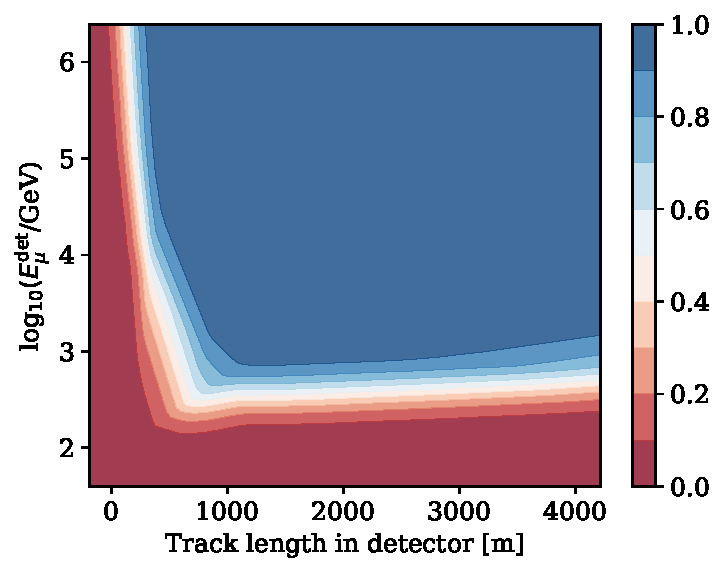
\includegraphics[width=0.75\textwidth]{img/trigger_rate_nn.pdf}
    \caption{缪子径迹型事件的筛选通过几率与缪子能量$E_\mu^\mathrm{det}$以及缪子在探测器内的穿行长度$L_\mu$的关系。}
    \label{fig:trigger_rate_nn}
\end{figure}

为中微子望远镜设计事件筛选算法是为了在存在高噪声的环境中筛选出像是有价值的信号\cite{KM3NeT_trigger:ICRC2019, IceCube_trigger:2015, KM3NeT_trigger:2018}。
在深海中运行的中微子望远镜会受到多种不同的噪声的影响:PMT的暗噪声($\lesssim 1 \,\mathrm{kHz} / \mathrm{PMT}$),海水的K40放射性衰变产生的切伦科夫光($\sim 2 \,\mathrm{kHz} / \mathrm{PMT}$)\cite{KM3NeT_K40:2017},有机物在受到扰动后激发出的光信号,深海鱼类发出的生物光信号\cite{ANTARES_biolumi:2021, Baikal_biolumi:2021}等等。

目前关于海铃探测器的研究尚处于早期阶段,我们对噪声对中微子信号分析的影响尚未完全考虑清楚。因此在以下的研究中,我们主要考虑一些信号强度比较高,不容易受到噪声影响的径迹型事件。我们在以下分析中将事件筛选的标准设置为:
\begin{enumerate}
    \item 事件中PMT探测到的NPE数量大于15。
    \item 经过重建算法后,重建得到的方向与真实中微子的方向之间的误差小于6度。
\end{enumerate}

通过模拟大量的缪子径迹型事件数据并对他们施加设计的事件筛选标准,再使用一个多层感知器来拟合筛选结果,我们可以通过训练得到通过筛选的几率与到达探测器的缪子能量$E_\mu^\mathrm{det}$以及缪子在探测器内的穿行长度$L_\mu$的关系如图\ref{fig:trigger_rate_nn}所示。


\subsection{对模拟事件的统计分析}

通过在探测器中注入大量的模拟事例,我们可以进行一些统计分析来检验事件产生器模拟程序的结果,同时,这也能加深对中微子望远镜探测到的事件分布的理解。
我们在$1\,\mathrm{TeV} - 10\,\mathrm{PeV}$的能量范围内,以谱指数为$-1.1$的能谱注入了400k个缪子中微子带电流事件。其中,有156k个事件中的缪子能够顺利到达探测器,而其他缪子或是因为中途就被介质所吸收,或是因为注入时没有对准探测器,导致没能在探测器中产生有效的信号。因此,在这一批次的模拟中,我们的事件产生器的命中率,或者说采样效率约为$40\%$。

图\ref{fig:sampling_energy_spectrum_unweighted}展示了在这一批模拟注入的事件中成功到达探测器的事件的初始中微子能量的分布。
可以看到我们在产生器中设置的$-1.1$的注入能谱使得在各个中微子能量范围内都有充足的事件分布。
同时我们也可以发现向下运动的中微子事件比向上运动的中微子事件在数量上要更多一些,这是因为向下注入时,海水的厚度和密度都比较小,缪子的能损程度较少,因此缪子有更大的几率能到达探测器。

\begin{figure}[!ht]%
    \centering
    \includegraphics[width=0.72\textwidth]{img/sampling_energy_spectrum_unweighted.pdf}
    \caption{模拟中成功注入的事件在中微子的能量和入射方向上的分布。}
    \label{fig:sampling_energy_spectrum_unweighted}
\end{figure}

\begin{figure}[!ht]%
    \centering
    \includegraphics[width=0.72\textwidth]{img/sampling_energy_spectrum.pdf}
    \caption{对于弥散的天体物理中微子流,在经过加权处理后,探测器在不同中微子的能量和入射方向上的事例率。}
    \label{fig:sampling_energy_spectrum}
\end{figure}

为了对探测器进行有物理意义的分析,我们需要把注入的事件与权重项$w_\mathrm{tot}$结合起来分析,同时我们还需要假设一个分析的物理能谱。
在本小节中,我们将研究对象定为弥散的全天各向同性的缪子中微子能谱,即我们将公式\ref{eq:diffse_nu_flux}中的谱指数和流强取为-2.35和1.45\cite{IceCube_diffse_muon:2021}。

图\ref{fig:sampling_energy_spectrum}中显示了在添加权重之后,探测器对不同的入射能量和方向的中微子的事例率。我们可以发现,随着中微子能量逐渐升高,探测到的事例率先上升后逐渐减少,在能量超过$10\,\mathrm{TeV}$后,它们的关系大致呈:
\begin{equation}
    \frac{\mathrm{d}N}{\mathrm{d}t\mathrm{d}E} \propto E_\nu^{-1.7}, 
    \label{eq:diffse_nu_mu_flux_observed}
\end{equation}
其中$\frac{\mathrm{d}N}{\mathrm{d}t\mathrm{d}E}$表示时间单位能量下探测器观测到的弥散缪子中微子流的事例率。


同时,我们也可以看到在经过加权后能够反映物理真实的事件分布中,在能量比较低时($E_\nu \lesssim 0.1\,\mathrm{PeV}$),入射方向向上的中微子的事例率与入射方向向下的事例率几乎没有差别。
而能量比较高($E_\nu > 1\,\mathrm{PeV}$)的情况下,入射方向向上的中微子事件比入射方向向下的中微子事件在事例率要小约2到10倍。
这种上下方向事件数的不对称是由一些几何效应引起的,几何效应主要包括两方面:宏观上地球的几何以及探测器附近的几何。

宏观上地球的几何导致向上和向下的中微子事件穿透地球的概率不同。随着能量的升高,中微子与物质的相互作用截面增大,地球的吸收作用使得大量向上运动的中微子在穿越地球的过程中就已经发生了反应。
不同能量不同入射角的中微子事件穿透地球的概率如图\ref{fig:survival_probability}所示。
从图中我们可以看到,能量大于$1\,\mathrm{PeV}$的中微子只有$\lesssim 0.1$的概率能够穿透地球。图中$\cos(\theta_z)=-0.85$处穿透率的突然变化是由于地球密度变化导致的,此入射角对应于中微子是否穿过密度最高的地核的分界线。


\begin{figure}[!htb]%
    \centering
    \includegraphics[width=0.75\textwidth]{img/survival_probability.pdf}
    \caption{不同能量$E_\nu$和不同天顶角$\theta_z$的中微子能够成功穿越地球的概率。}
    \label{fig:survival_probability}
\end{figure}

探测器附近几何结构的影响是指在缪子径迹的长度范围内(对于海水而言约$\sim 10\,\mathrm{km}$),介质密度的变化。在模拟中,我们将中微子望远镜阵列的中心放置在水下$2900\,\mathrm{m}$处,因此沿望远镜中心向上$2900\,\mathrm{m}$即到达了海水和空气的交界面,向下$500\,\mathrm{m}$便是海水和岩石的交界面。
如图\ref{fig:sampling_dis_position}所示,向上的缪子中微子事件可以来自地壳深处约$4\,\mathrm{km}$处,而向下的缪子事件由于受到水深的限制,最多只能来自于$2900\,\mathrm{m}$外的海水中,因此向上的事件可供中微子发生DIS反应的靶物质质量要大于向下的事件。
然而虽然向上的事件拥有更大的可反应物质量,但其产生的缪子在介质中穿行时会损失更大的能量。
在图\ref{fig:sampling_energy_spectrum_det}中,我们观察到在选取了高能($E_\nu > 1\,\mathrm{PeV}$)的中微子事件之后,向下运动的中微子事件通常拥有更高的到达探测器的能量,而向上运动的中微子事件在到达探测器的能量上更加的弥散。这种效应会导致向上运动的中微子事件对原初中微子的能量重建的效果较差,因为我们难以知道缪子究竟在探测器外损失了多少的能量。

\begin{figure}[!htb]%
    \centering
    \includegraphics[width=0.75\textwidth]{img/sampling_dis_position.pdf}
    \caption{向上运动和向下运动的事件各自的DIS反应顶点在探测器坐标系下的$z$坐标$z_\mathrm{DIS}$上的分布。其中,绿色的点虚线表示海水与岩层的分界线,红色的点虚线表示海水与空气的分界线。}
    \label{fig:sampling_dis_position}
\end{figure}


\begin{figure}[!htb]%
    \centering
    \includegraphics[width=0.75\textwidth]{img/sampling_energy_spectrum_det.pdf}
    \caption{在选取了$E_\nu > 1\,\mathrm{PeV}$的事件之后,向上运动和向下运动的事件到达探测器的能量的分布图。}
    \label{fig:sampling_energy_spectrum_det}
\end{figure}

图\ref{fig:sampling_zenith}展示了不同能量的中微子事件在入射的天顶角$\theta_z$空间下的分布情况。我们可以看到,除了上文中提到的上下几何不对称以外,在能量比较低($E_\nu < 100\,\mathrm{TeV}$)的情况下,水平方向的中微子事件要明显少于其他方向上的事件。这是因为我们的探测器构造像是薄饼状:在水平方向上延展比较宽,半径达到$2\,\mathrm{km}$,而在垂直方向上高度比较小,仅为$0.6\,\mathrm{km}$。这导致了我们探测器接对来自水平方向的事件的有效面积相比于垂直方向有所降低。

\begin{figure}[!htb]%
    \centering
    \includegraphics[width=0.75\textwidth]{img/sampling_zenith.pdf}
    \caption{不同能量的中微子事件在入射天顶角空间下的分布。}
    \label{fig:sampling_zenith}
\end{figure}

\subsection{有效面积计算}

在介绍完蒙特卡洛采样中有关采样和事件权重的内容之后,我们可以回到一开始的有效面积计算公式\ref{eq:eff_area_init}中。公式中的$\frac{\mathrm{d}N}{\mathrm{d}t ~\mathrm{d}\Omega ~\mathrm{d}E}(E, \hat{n})$项可以通过将公式\ref{eq:sampling_trigger_rate}微分化得到,而微分操作对应到蒙特卡洛方法中便是对样本进行分区间计算:
\begin{equation}
    \frac{\mathrm{d}N}{\mathrm{d}t \mathrm{d}E \mathrm{d}\Omega} = 
    \frac{1}{N_\mathrm{tot} \Delta E \Delta\Omega} \sum_{i \in \mathrm{bin}} \left[ 
    \mathrm{I}_\mathrm{sel}(s_i) \times 
    F_\mathrm{phy} (E_i, \hat{n}_i) \times
    w_{\mathrm{tot}, i} \right] ,
\label{eq:sampling_trigger_rate_diff}
\end{equation}
其中$\sum_{i \in \mathrm{bin}}$表示对属于该能量和立体角范围区间内的事件进行求和,$\Delta E \Delta\Omega$表示区间的相空间大小。

将公式\ref{eq:sampling_trigger_rate_diff}代入到公式\ref{eq:eff_area_init}中可以得到:
\begin{equation}
    A_\mathrm{eff} (\hat{n}, E) = \frac{1}{N_\mathrm{tot} \Delta E \Delta\Omega} \sum_{i \in \mathrm{bin}} \left[ 
    \mathrm{I}_\mathrm{sel}(s_i) \times 
    w_{\mathrm{tot}, i} \right] ,
    \label{eq:eff_area}
\end{equation}
这里,我们已经成功地从有效面积的表达式中约去了中微子源的物理流量$F_\mathrm{phy} (E, \hat{n})$。我们可以看到$A_\mathrm{eff} (\hat{n}, E)$与具体的中微子流量无关,而与探测器的对事件的探测能力$\mathrm{I}_\mathrm{sel}(s_i)$以及中微子的物理性质$w_{\mathrm{tot}, i}$有关,它反应的是探测器对某一种事件类型的探测能力。

通过模拟,我们得到探测器的有效面积与中微子的能量$E_\nu$和入射天顶角$\theta_z$之间的关系如图\ref{fig:eff_area}中所示。
在将$\theta_z$分为向上入射($-1 \leq \theta_z < -0.5$),水平入射($-0.5 \leq \theta_z < 0.5$)和向下入射之后($0.5 \leq \theta_z < 1$)之后,我们对不同入射角区间的有效面积求平均,可以得到图\ref{fig:eff_area_band}中所示的结果。

从图\ref{fig:eff_area_band}中我们可以观察到,对于水平和向下入射的中微子而言,当中微子能量达到$10\,\mathrm{PeV}$时,海铃中微子望远镜的有效面积可以达到$5 \times 10^3\,\mathrm{m^2}$,是IceCube的5倍多\cite{IceCube_10yr_point_source:2019}。
对于向上入射的中微子而言,当中微子的能量达到$100\,\mathrm{GeV}$时,有效面积达到顶峰,约为$10^3\,\mathrm{m^2}$。当能量继续升高时,地球的吸收效应导致有效面积逐渐降低,在$10\,\mathrm{PeV}$时约为$10^2\,\mathrm{m}^2$。

\begin{figure}[!htb]%
    \centering
    \includegraphics[width=0.90\textwidth]{img/eff_area.pdf}
    \caption{探测器的有效面积与入射中微子的能量以及天顶角之间的关系。}
    \label{fig:eff_area}
\end{figure}

\begin{figure}[!htb]%
    \centering
    \includegraphics[width=0.65\textwidth]{img/eff_area_band.pdf}
    \caption{不同入射的天顶角下,探测器的有效面积与入射中微子能量的关系。}
    \label{fig:eff_area_band}
\end{figure}

\section{对中微子源的灵敏度}

有了探测器的角度分辨率和有效面积之后,我们便可以开始计算探测器对中微子源的灵敏度。在本章节的灵敏度分析中,我们通过来自地球方向,向上穿行的径迹型事件来寻找中微子的源,即要求天顶角$\theta_z > 85^\circ$,选择这样的事件通道是为了避免数量众多的大气缪子本底的影响。

\subsection{天体源赤纬的影响}

由于探测器的有效面积是与中微子的入射角相关的,因此我们要首先讨论一下来自某一个天体物理中微子源的流量相对于探测器的入射角。
与IceCube那样位于南极点的探测器不同,海铃所处的纬度位置为$16^\circ 8' \mathrm{N}$,因此,它会随着地球的自转而转动。
在海铃看来,宇宙中固定位置的天体物理源在不同的时刻对应的天顶角是不同的:
\begin{equation}
\begin{aligned}
    \cos\theta_z(t) &= \hat{n}_s \, \cdot \, \hat{n}_\mathrm{det}(t) \\
    \hat{n}_\mathrm{det}(t) &= \left(\cos(l_\mathrm{det})\cos(\frac{2\pi t}{T}),\,
    \cos(l_\mathrm{det})\sin(\frac{2\pi t}{T}),\, 
    \sin(l_\mathrm{det}) \right) ,
\end{aligned}
\end{equation}
其中$\hat{n}_s$是该天体物理源在赤道坐标系中的方位,$\hat{n}_\mathrm{det}(t)$表示探测器在赤道坐标系中的方位,它会随着地球的转动而变化。
$l_\mathrm{det}$表示探测器的纬度,$t$表示时间,$T$表示地球的自转周期,即一天。

在各个赤纬天区中,典型的高能天体物理源相对于海铃的入射角随时间的变化曲线$\cos\theta_z(t)$如图\ref{fig:source_zenith_time_curve}所示。
在地球自转一圈的时间中,来自不同赤纬上的天体物理源可以被海铃所观测的时间占总事件的比例如图\ref{fig:source_zenith_duty_cycle}中所示。
从图中可以发现,除了北极点附近赤纬范围内的少数区域外,海铃对大多数天体中微子源都能有较长的观测时间窗口。

\begin{figure}[!htb]%
    \centering
    \includegraphics[width=0.60\textwidth]{img/source_zenith_time_curve.pdf}
    \caption{几个潜在的天体物理源在海铃中微子望远镜视角的天顶角随时间的变化。图中选取了北天,赤道和南天各3个源,它们在赤道坐标系下的坐标分别为:NGC 1068:$(\mathrm{02^h 42^m, 00^\circ 00′})$,LHAASO 1825-1326:$(\mathrm{18^h 25^m, -13^\circ 26′})$,Crab:$(\mathrm{05^h 34^m, +22^\circ 00'})$}
    \label{fig:source_zenith_time_curve}
\end{figure}

\begin{figure}[!htb]%
    \centering
    \includegraphics[width=0.60\textwidth]{img/source_zenith_duty_cycle.pdf}
    \caption{海铃中微子望远镜对不同赤纬的天体物理源的可观测时间占比(蓝线)以及在可观测时间中,水平方向的占比(红线)。其中我们将水平方向定义成$100^\circ<= \theta_z <85^\circ$。图中横坐标表示天体物理源的赤纬的正弦值。}
    \label{fig:source_zenith_duty_cycle}
\end{figure}

在图\ref{fig:eff_area}中,我们的有效面积是以探测器为中心的,其横轴表示中微子事件相对于探测器的天顶角。现在,我们以中微子源为考虑对象,定义探测器对不同赤纬的中微子源的有效面积$A_\mathrm{eff}^s$:
\begin{equation}
    A_\mathrm{eff}^s(E_\nu, \delta_s) = \frac{1}{T} \int_0^T A_\mathrm{eff}(E_\nu, \theta_z(t)) \times \mathrm{I}_\mathrm{up}(\theta_z(t)) \, \mathrm{d} t \,   ,
\end{equation}
其中,积分范围$T$表示一天,$\mathrm{I}_\mathrm{up}(\theta_z(t))$表示筛选向上穿行的缪子事件。
这种有效面积的计算方式考虑了该天体物理源在一天的时间内相对于探测器的天顶角的平均效应。

海铃对向上穿行的事件的有效面积如图\ref{fig:eff_area_with_lat}中所示。
可以可以看到,相比于图\ref{fig:eff_area},相对于源的有效面积整体降低了约一半,这是因为探测器的平均可观测时间占比变成了约50\%。
并且在高能处,探测器的有效面积降低得尤其明显,这是因为我们要求中微子事件是向上穿行的,而高能的中微子事件在向上穿行的过程中会经历强烈的地球吸收作用。
而且赤纬范围在$-0.7 < \sin(\delta_s) < 0.7$范围内的源在高能段衰减地比其他赤纬范围要更加明显,这是因为如图\ref{fig:source_zenith_duty_cycle}中所示,在它们的可观测时间中,水平入射的占比很少。
探测器对北极附近的源会有更弱的有效面积,而对于南极的附近的源会有更好的有效面积,与图\ref{fig:source_zenith_duty_cycle}中的探测器可观测时间占比一致。

\begin{figure}[!htb]%
    \centering
    \includegraphics[width=0.80\textwidth]{img/eff_area_with_lat.pdf}
    \caption{海铃中微子望远镜对不同赤纬的天体物理源的有效面积,图中横坐标表示赤纬的正弦值。}
    \label{fig:eff_area_with_lat}
\end{figure}



\subsection{对NGC 1068的显著性}

对于某一假定的中微子天体物理源,我们可以通过分析来自该源的中微子事件在立体角空间上相对于背景事件的超出来计算望远镜对它观测的显著性。
以NGC 1068这个IceCube列表中最有可能的源为例,我们假设源的流强$F_\mathrm{NGC}(E_\nu)$为IceCube的最佳拟合结果\cite{IceCube_NGC1068:2022}。
我们分析中的背景主要包括弥散的中微子辐射背景$F_\mathrm{diff}(E_\nu)$和大气中微子背景$F_\mathrm{atm}(E_\nu)$。
对于这两种背景的流强以及不确定性,我们分别参考了IceCube对弥散缪子中微子流强的观测\cite{IceCube_diffse_muon:2021}和大气中微子的观测\cite{IceCube_atmos_nu:2014}。
上述信号和背景的中微子流强的能谱如图\ref{fig:source_background_flux}中所示。

\begin{figure}[!htb]%
    \centering
    \includegraphics[width=0.70\textwidth]{img/source_background_flux.pdf}
    \caption{IceCube测得的NGC 1068的中微子的流强,弥散天体物理中微子的流强,以及大气中微子的流强,阴影区域表示背景流强的不确定性。注意,图中NGC 1068源是一个点源,其流强单位为$\mathrm{GeV^{-1} cm^{-2} s^{-1}}$,而弥散天体物理中微子和大气中微子流强的单位中包含每立体角,为$\mathrm{GeV^{-1} cm^{-2} s^{-1} sr^{-1}}$。}
    \label{fig:source_background_flux}
\end{figure}

将中微子源流强的能谱与探测器的有效面积做卷积,可以得到探测器探测到的事例率:
\begin{equation}
\begin{aligned}
    \frac{\mathrm{d}N_s}{\mathrm{d}t} &= \int F_s(E_\nu)  A_\mathrm{eff}^s (E_\nu, \delta_s) \,\mathrm{d} E_\nu \\ 
    \frac{\mathrm{d}N_\mathrm{b}}{\mathrm{d}t} &= \Delta \Omega \int F_\mathrm{b}(E_\nu)  A_\mathrm{eff}^s (E_\nu, \delta_s) \,\mathrm{d} E_\nu, \\
\end{aligned}
    \label{eq:event_rate_using_eff}
\end{equation}
其中的$F_s(E_\nu)$表示天体物理源的中微子流量,其量纲为单位时间单位面积的事件数量,注意量纲中不含有立体角。
而对于弥散的中微子流强$F_b(E_\nu)$,由于其流强量纲中含有立体角,因此在计算实例率时需要再乘以$\Delta\Omega$,用于表示对某一中微子天体源中分析时所选取的立体角空间范围。
注意,为了将信号事件全部包含在内,$\Delta\Omega$应当大于探测器的角分辨率。

我们选取观测的半张角的余弦变化值$\Delta\cos\theta_s$为$5\times 10^{-4}$时的角度为观测区域,其对应的半张角为$1.81^\circ$。
在该区域中,我们以$1\,\mathrm{TeV}$为中微子流强能谱作低能截断,模拟中微子望远镜对来自点源的中微子事件的响应。
我们以一年为曝光时间来计算在选取的半张角区域内信号和背景事件的事例率的期望值,其结果如图\ref{fig:event_rate_around_source}中下图所示。
我们可以看到由于中微子信号来自于一个点源,因此方向重建得到的信号事件的角度分布主要集中在0附近,它的扩展反应的是探测器的角度分辨率。
而弥散的背景中微子的方向在点源附近的立体角空间内是均匀分布的,因此经过重建之后在$\Delta\cos\theta_s$相空间中的分布也是均匀的。
我们可以看到,在当前的信号和背景流强假设下,我们对NGC-1068的方向上能够观测到明显的事例率超出。

值得注意的是,我们在本次灵敏度分析时只在中微子方向的相空间中寻找信号超出,而没有考虑中微子能量的相空间,这是因为目前我们还没有完成对径迹型事件的能量重建工作。
对于中微子的能量,我们只用它设置的信号和背景选取的能量阈值,能量阈值的选取对分析结果会有重要的影响,这会在后续内容会有更多的讨论。

\begin{figure}[!htb]%
    \centering
    \includegraphics[width=0.70\textwidth]{img/event_rate_around_source.pdf}
    \caption{在$\Delta\cos\theta_s$属于0到$5\times 10^{-4}$的张角范围内,中微子信号和背景事件在方向空间中的事例率的对比。其中信号中微子是来自于NGC 1068源,其能谱指数假设为-3.2。背景中微子是来自于大气中微子和弥散高能中微子。}
    \label{fig:event_rate_around_source}
\end{figure}

接下来,我们来计算该事例率和立体角的分布下,中微子望远镜对NGC 1068源的显著性是多少。
在计算中,我们采用了分区间的似然估计(binned likelihood analysis):
\begin{equation}
\begin{aligned}
    \mathcal{L}(n_s, n_b;\mu, \vec{n}) &=  
    \prod^N_{i=1} \frac{(\mu n_s p_i^s + \mu n_b p_i^b)^{n_i}}{n_i!} 
    e^{-(\mu n_s p_i^s + \mu n_b p_i^b)}
    \times \frac{1}{\sqrt{2\pi}\sigma_b} e^{-\frac{(n_b-n_b^0)^2}{2\sigma_b^2}} \\
    \ln{\mathcal{L}}(n_s, n_b;\mu, \vec{n}) &= 
    -\mu(n_s+n_b) + \sum^N_{i=1} n_i \ln (\mu n_s p_i^s + \mu n_b p_i^b) 
    - \frac{(n_b-n_b^0)^2}{2\sigma_b^2} + C ,
    \label{eq:binned_likelihood}
\end{aligned}
\end{equation}
公式中的第一部分表示每一个区间内的泊松涨落,其中$n_s$和$n_b$表示信号和背景事件的总事例率,在我们的应用中,$n_s$和$n_b$分别表示NGC 1068的事例率和大气中微子以及弥散中微子在$\Delta\cos\theta_s < 5\times 10^{-4}$范围内的总事例率。
$\mu$表示观测的时间,公式中出现的$\mu n_s$和$\mu n_b$表示在观测时间$\mu$下,探测到的总的信号和背景的事件数的期望值。
$n_i$表示观测到的第$i$个区间内的事件数量,$p_i^s$,$p_i^b$分别表示模型中信号和背景在第$i$个区间内的分布概率,在我们的应用中,信号的分布表征着中微子望远镜的角分辨率,而背景是弥散的均匀分布的。$N$是区间的总数。
公式中的第二部分表示对背景事例率偏离模型预测值的惩罚,其中$n_b^0$和$\sigma_b$分别表示我们的模型中对背景事例率的期望和涨落,在我们的应用中,表示IceCube对大气中微子和弥散中微子的测量值和误差。

在对信号的显著性分析中,我们探究一个观测到的信号有多少的可能性是由背景涨落导致的。
在这种情况下,我们假设既观测到了信号又观测到了背景,那么观测到的数据在每一个区间中都应该服从期望为$\mu(n_s p_i^s +  n_b^0 p_i^b)$的柏松分布。
在具体操作中,我们使用了Asimov近似\cite{Cowan_Asimov_estimate:2010},即使用了观测值的期望来代替原本应当是随机分布的观测值:
\begin{equation}
    n_i = \mu(n_s p_i^s +  n_b^0 p_i^b) ,
    \label{eq:asimov_est_signal}
\end{equation}
这样可以避免繁琐的模拟抽样过程,适合在预研阶段对显著性进行快速的估计。

我们研究这样的观测信号有多少可能性是由纯背景所贡献的,因此我们定义如下的检验统计量(test statistics,TS):
\begin{equation}
    \mathrm{TS}(\mu) = 2 \ln \left( \frac
    {\mathcal{L}(\mu n_s, \mu n_b^0; \vec{n})} 
    {\mathcal{L}(0, \mu \hat{n}_b; \vec{n})} \right) ,
    \label{eq:ts_significance}
\end{equation}
其中$\mathrm{TS}(\mu)$表示观测时间$\mu$下的TS值,$\hat{n}_b$表示使得$\mathcal{L}(0, \mu n_b; \vec{n})$达到最大的背景事例率。

这样定义的TS中,只有$n_b$这一个自由参数被最大化了,因此TS应当服从自由度为1的卡方分布\cite{Cowan:1998}:
\begin{equation}
    \mathrm{TS} \sim \chi^2(1)
\end{equation}
代入公式\ref{eq:asimov_est_signal}中Asimov近似下观测的事件数的期望,可以得到TS值,并且我们可以根据卡方检验中的概率分布来得到该TS值对应到标准高斯分布$\mathcal{N}(x)$中的显著性$\sigma$:
\begin{equation}
    \int^\infty_\mathrm{TS} \chi^2(x, 1) \mathrm{d}x = 
    2 \int^\infty_\sigma \mathcal{N}(x) \mathrm{d}x ,
    \label{eq:ts_to_sigma}
\end{equation}

最终计算到显著性关于观测时间的函数$\sigma(\mu)$如图\ref{fig:ngc_significance_time_curve}中所示。
在图中,我们绘制了几条不同能量筛选阈值下显著性结果,可以看到在$1\,\mathrm{TeV}$和$3.2\,\mathrm{TeV}$的能量阈值下,海铃可以在约0.5年的观测时间内就以$5\sigma$的置信度发现NGC 1068这个源。
而如果能量阈值选取到$10\,\mathrm{TeV}$,则需要约1.5年的时间才可以达到$5\sigma$。
这是由于NGC 1068源的谱指数为-3.2,比弥散的高能中微子流更软,它的主要中微子信号都集中在$1\,\mathrm{TeV}$到$10\,\mathrm{TeV}$能段。
从图\ref{fig:event_rate_around_source_energy_threshold}中可以看到,当能量阈值取到$10\,\mathrm{TeV}$时,总事例率将降低到约4个事件每年,尽管此时背景事例率非常稀少,但在如此低的事例率下仍然难以实现高置信度。

如果我们在分析中加入对中微子能量重建的不确定度,在这个能段径迹型缪子中微子的能量重建的不确定度在对数空间中大约有0.5到1个量级左右。加入能量重建在一方面将会使我们上述分析中的能量阈值出现一定的波动,造成信号的显著性降低。
而另一方面,加入中微子能量的分析可以使我们做信号关联的相空间从单个立体角的维度扩充到立体角加上能量的维度,这可以在一定程度上提高信号显著性。
因此我们可以合理地推测,即便考虑了能量重建的影响,海铃仍然能够在$\lesssim 1$年的时间内以$5\sigma$的置信度发现NGC 1068这个源。

\begin{figure}[!htb]%
    \centering
    \includegraphics[width=0.55\textwidth]{img/ngc_significance_time_curve.pdf}
    \caption{海铃中微子望远镜观测到NGC 1068源在不同的中微子能量阈值截断下的显著性随时间变化的曲线。}
    \label{fig:ngc_significance_time_curve}
\end{figure}

\subsection{全天中微子源的灵敏度与显著性分析}

在本小节中,我们探讨海铃对来自全天的各个方向的源的灵敏度。我们将望远镜的观测时间固定为10年,假设天体物理源辐射中微子的能谱指数为-2并选取$40\,\mathrm{TeV}$来作为事件筛选的能量阈值,观察对于来自各个不同赤纬的源而言,其流量需要达到多少才能满足以$5\sigma$的置信度发现源的信号的要求。
我们将$5\sigma$发现流量阈值与源的赤纬的曲线称为望远镜的$5\sigma$显著性曲线,其分析结果如图\ref{fig:all_sky_sensitivity_E2}中的红色实线所示,图中同样展示了其他望远镜的$5\sigma$显著性曲线。
可以看到在南天区($\sin(\delta)<0$),海铃的的$5\sigma$显著性曲线相较于IceCube要低约两个量级,在北天区($\sin(\delta)>0$),海铃也比IceCube要低5-6倍。

而如果我们将源的能谱指数改成更软的$-3$能谱,并且选取$1\,\mathrm{TeV}$来作为事件筛选的能量阈值,分析得到$5\sigma$显著性曲线将如图\ref{fig:all_sky_sensitivity_E2}中所示。

\begin{figure}[!htb]%
    \centering
    \includegraphics[width=0.65\textwidth]{img/all_sky_sensitivity_E2.pdf}
    \caption{海铃探测器10年数据累积下的全天点源的90\%灵敏度曲线(虚线)和$5\sigma$显著性曲线(实线)。世界上的其他中微子望远镜望远镜:IceCube\cite{IceCube_10yr_point_source:2019},IceCube-Gen2\cite{IceCube-Gen2_sensitivity:2021}和KM3NeT\cite{KM3NeT_sensitivity:2018}的数据也展示了在图中,其中KM3NeT的数据是从6年的观测时间放大到10年的观测时间得到的,假设显著性和灵敏度都随着时间的平方增长。在分析中,我们假设源的能谱指数为-2,对中微子事件筛选的能量阈值为$40\,\mathrm{TeV}$。}
    \label{fig:all_sky_sensitivity_E2}
\end{figure}

\begin{figure}[!htb]%
    \centering
    \includegraphics[width=0.65\textwidth]{img/all_sky_sensitivity_E3.pdf}
    \caption{类似于图\ref{fig:all_sky_sensitivity_E2},但是,假设源的能谱指数为-3,对中微子事件筛选的能量阈值为$1\,\mathrm{TeV}$。}
    \label{fig:all_sky_sensitivity_E3}
\end{figure}

除了$5\sigma$显著性曲线以外,衡量探测器寻找天体物理源的另外一个重要属性是90\%灵敏度曲线。
90\%灵敏度表示在纯背景假设下,需要多强的流量才能使得信号能够以90\%的几率超出背景。
通常而言90\%灵敏度曲线对中微子流量的要求会比$5\sigma$显著性曲线要低半个多量级,因为前者表示探测器有可能能发现源的信号超出迹象,而后者要求探测器信号超出要达到非常高($5\sigma$)的显著性。
在分析计算90\%灵敏度时,我们假设只观测到了背景,那么观测到的数据在每一个区间中的数量$\mu(n_b^0 p_i^b)$(使用Asimov近似)。
我们将TS定义为:
\begin{equation}
    \mathrm{TS}(\mu) = 2 \ln \left( \frac
    {\mathcal{L}(0, \mu n_b^0; \vec{n})} 
    {\mathcal{L}(\mu n_s, \mu \hat{n}_b; \vec{n})} \right) ,
    \label{eq:ts_sensitivity}
\end{equation}
其中$\hat{n}_b$表示使得$\mathcal{L}(\mu n_s, \mu n_b; \vec{n})$达到最大的背景事例率。
同样的,$\mathrm{TS}(\mu)$会符合自由度为1的卡方分布,我们寻找能够使得:
\begin{equation}
    \int^\infty_\mathrm{TS} \chi^2(x, 1) \mathrm{d}x = 10\% ,
    \label{eq:ts_to_90}
\end{equation}
的信号事例率,并将之转换为流强,即能够得到90\%灵敏度所对应的信号流强。
对于能谱指数为-2和-3的源,海铃的90\%灵敏度曲线分别如图\ref{fig:all_sky_sensitivity_E2}和图\ref{fig:all_sky_sensitivity_E3}中红色虚线所示。


    \chapter{优化中微子望远镜设计}
\label{chap:telescope_design}

\section{使用hDOM来提升角分辨率}
\label{sec:hdom}

海铃中微子望远镜的一大特点是使用了全新的hDOM\cite{hDOM:2021}来作为其探测切伦科夫光的模块,它即包含传统的PMT,又包含新型的光敏元件——SiPM(silicon photon multiplier)。

\subsection{SiPM的特点}

SiPM是一种硅基的光敏探测元件,它是由成百上千个处于盖革工作状态下的雪崩光电二极管(photon avalanche diodes,PAD)所铺设构成的\cite{understanding_sipm:2019}。由于这些PAD处于盖革工作状态,即当有一个光子到达其表面,激发出电子空穴对时,便能在外部电场的作用下形成雪崩效应,因此它们也被称为SPAD(single photon avalanche diodes)。
相比于传统的PMT,SiPM具有许多独特的优点:
\begin{enumerate}
    \item SiPM中的SPAD内部的尺寸结构很小,其内部的雪崩发展及其迅速而稳定,因此SiPM拥有极佳的时间响应性能,理论上可以达到$\sim 10\,\mathrm{ps}$。而PMT中光子需要经过多个倍增极的放大,因此有$10 ~ 20\,\mathrm{ns}$的渡越时间(transient time,TT),而渡越时间弥散(transient time spread,TTS)通常在$1~5\,\mathrm{ns}$量级。
    \item SiPM中的SPAD通过光子激发电子空穴对的量子效率可以达到$\gtrsim 50 \%$,而PMT中借助光子激发出能够离开阴极材料的自由电子的量子效率仅为$\sim 30\%$。
    \item SiPM中的SPAD对单光子响应产生的电流大小非常稳定,因而具有很好的单光子分辨能力。
    \item SiPM中的PAD只需要加上几个伏特的偏置电压即可处于盖革工作模式,达到预设的量子效率和增益效果。而PMT则需要加上$\gtrsim 1000 \,\mathrm{V}$的高压才能达到稳定的增益,因而需要在探测器内部添加额外的升压电路模块,。
    \item 作为一种硅基的固态探测器,SiPM是的仪器体积小集成程度高,可以搭载在各种不同的探测设备上。而PMT是一个真空玻璃管,更容易受到损坏,日本的神冈探测器就曾经因为PMT真空管爆炸引发连锁反应,直接毁掉了近半个探测器的PMT。为防止类似事件的发生,JUNO中的PMT外部均额外安装了保护壳\cite{JUNO_pmt_implosion:2022}。
    \item 在批量生产下,SiPM作为一种硅基晶体材料,可以在流水线的形式快速地加工出来,因而可以有效降低成本。而PMT的制造过程中依赖于许多人力帮助,批量生产的效率并不高。
\end{enumerate}

当然,SiPM也有其自身的缺点,其最大的问题便是在室温下噪声非常地高。SiPM中由于晶体自身的结构缺陷,很容易通过热涨落的形式产生暗噪声,常见的型号在室温下噪声率在$100\,\mathrm{kHz/cm^2}$的量级。
此外SiPM内部的串扰也相对较大,一个雪崩的SPAD可能会激发与之相邻的SPAD,从而对一个单光子事件产生多光子的响应信号。

由于这些特点,SiPM目前已经在雷达激光测距(LIDAR)\cite{sipm_lidar:2013},医学造影\cite{nuclear_medical_imaging:2009},JUNO-TAO探测器\cite{JUNO-TAO:2023},对撞机的闪烁体探测器\cite{SiPM_CEPC:2020}等多个领域都有所应用。
在本节后续的内容中,我们将讨论SiPM在中微子望远镜中的潜在应用。

\subsection{hDOM性能分析}

在本研究中,我们主要考虑SiPM的快速时间响应能力和高量子效率对中微子望远镜中的径迹方向重建精度的提升。
我们以KM3NeT的mDOM设计为基础结构\cite{KM3NeT_mDOM:2015},在其中额外加入了24个SiPM阵列,每一个SiPM阵列由$9 \times 9$个SiPM单点构成,有$2.7\times 2.7\,\mathrm{cm}$的面积,它们组成了4个水平的环带,插入在PMT中间。
我们将24个SiPM和31个PMT同时加入到数字光学模块中,构成了一个混合数字光学模块(hDOM),其初步设计图如图\ref{fig:hDOM_rendering}中所示。

为了研究量子效率和时间分辨率对探测器性能的影响,我们在模拟中假设了三种不同的光敏探测器,其参数列表分别如表格\ref{tab:sensor_parameters}中所示。

\begin{table} [htbp]
    \centering
    \begin{tabular}{c|c|c|c}
        \hline
        光敏元件 & PMT & toy SiPM & SiPM  \\
        \hline
        物理体积 [$\rm{cm}^2$] & 40.7  & 40.7 & 7.3 \\
        \hline
        $405\,\mathrm{nm}$下光子探测效率 [\%] & 24 & 24 & 42 \\
        \hline
        时间分辨率 [$\rm{ns}$] & 5 & 0.1 & 0.1 \\
        \hline
    \end{tabular}
    \caption{三种不同的探测元件的性能参数}
    \label{tab:sensor_parameters}
\end{table}

使用这些不同的光敏元件,我们可以组件如下所示的三种不同的光学模块的配置:
\begin{enumerate}
    \item 配置A,由31个PMT构成的光学模块,即形如KM3NeT的mDOM。
    \item 配置B,由31个物理面积和量子效率与PMT相同,但是拥有极佳时间分辨性能的toy SiPM(或者也可以称为是高时间分辨率的PMT)构成的光学模块。
    \item 配置C,由31个PMT和24个标准的SiPM所构成的混合光学模块,即我们的hDOM。
\end{enumerate}
其中,我们的hDOM拥有适中的时间分辨率和最大的光敏面积。利用章节\ref{subsec:hDOM_sim}介绍过的模拟程序,我们模拟了hDOM对来自不同方向的平行光的响应,其内部各个光敏元件所对应的有效光子接收面积如图\ref{fig:hdom_effective_area}中所示。

\begin{figure}[!htb]%
    \centering
    \includegraphics[width=0.90\textwidth]{img/hdom_effective_area.pdf}
    \caption{hDOM中各个光敏元件组分的有效光子接收面积随光子入射角的关系。}
    \label{fig:hdom_effective_area}
\end{figure}

在完成对光敏元件的假设和构建完光学模块之后,我们研究的主要内容便是探讨不同的光敏模块对径迹型事件的响应,其中我们着重关心在不同光敏模块配置下阵列对缪子径迹的角度分辨率。

为提高模拟的效率,我们配置了一个相对紧凑的$1\,\mathrm{km^3}$体积的阵列,它在$x$,$y$和$z$方向上分别均匀得分布着$10 \times 10 \times 50$个光学模块,总共包含了5000个光学模块。
我们将介质的光学性质分别设置成深海海水和南极冰川冰,其中南极冰川比相对于深海海水具有更长的吸收长度和更短的散射长度\cite{OP_IceCube:2013, OP_KM3NeT_LAMS:2011}。对着两种介质,我们分别进行了模拟,从而比较不同配置的光学模块在不同介质下的表现。

我们在探测器阵列中注入了大批量的$1\,\mathrm{TeV}$的缪子径迹型数据,在模拟得到切伦科夫光子打在光学模块表面的光子击中信息后,我们利用我们设计的hDOM模拟程序分别模拟不同光学模块配置下,光敏元件对入射光子的响应。
随后我们根据表\ref{tab:sensor_parameters}中的配置来模拟光敏元件对光子的探测效率和时间测量精度,并最终用章节\ref{sec:angular_resolution}中介绍的径迹重建算法来对径迹型事件进行重建,根据重建结果得到阵列的角分辨率。

我们的模拟和重建结果显示,对于$1\,\mathrm{TeV}$的缪子径迹型事件而言,不同配置下的探测器对缪子信号的重建精度如图\ref{fig:hdom_angular_resolution_total}中所示。
我们发现在海水中相比于普通的mDOM(配置A),hDOM(配置C)能够带来$\sim40\%$的角度分辨率提升。而通过对比普通的mDOM(配置A)和由toy SiPM构成的DOM(配置B),我们可以发现,光敏元件的时间分辨率对角度重建性能有至关重要的影响。
与此同时,在冰介质中,hDOM(配置C)和由toy SiPM构成的DOM(配置B)相比于普通的mDOM(配置A)的提升并不明显,仅为$\sim 10\%$的量级。这是由于冰介质中的散射效应明显,因此光子到达时间的测量实际上是由散射效应所主导的,而非光敏元件自身的时间分辨率。

我们的研究表明SiPM的高时间精度和高量子效率的特点可以极大地提高中微子望远镜阵列的角度分辨率。
但是在真实的中微子望远镜阵列中,还有一些其他因素会影响hDOM的时间精度:
阵列的时钟同步性能,目前我们计划使用的小白兔系统\cite{white_rabbit:2013}大约能提供$< 100 \,\mathrm{ps}$的时钟同步精度;
hDOM的定位精度,KM3NeT的声学定位系统\cite{KM3NeT_acoustic:2022}可以达到$\sim 10 \,\mathrm{cm}$的定位精度,对应$\sim 400 \mathrm{ps}$的光子传播时间;
由海水色散关系导致的切伦科夫光的到达时间弥散等等。
对于这些实验中需要考虑的情形,我们还需要更多的研究才能准确地确定hDOM的性能优势。


\begin{figure}[!htb]%
    \centering
    \includegraphics[width=0.95\textwidth]{img/hdom_angular_resolution_total.pdf}
    \caption{不同配置下的光学模块对$1\,\mathrm{TeV}$的缪子径迹型事件的重建角分辨率。左图为在深海海水中的情况,而右图对应在南极冰川冰中的情况。}
    \label{fig:hdom_angular_resolution_total}
\end{figure}





\section{彭罗斯构型来作为串列单元的排布}

\subsection{彭罗斯构型介绍}

海铃中微子望远镜的串列单元的几何布局设计中采用了彭罗斯构型,在不考虑机器人过道后,阵列的布局如图\ref{fig:geo_layout_penrose}所示。
在彭罗斯构型中,串列单位的位置对应于彭罗斯镶嵌中的多边形的顶点位置,而彭罗斯镶嵌是一种非周期性密铺\cite{tilings_and_patterns:1987},其形状如图\ref{fig:Penrose_tiling_wiki}中所示。
彭罗斯镶嵌的最大特点是它不具备平移周期性,因此从宏观上看,空间中的每一个点都与其他的点周围的结构互不相同的。
尽管如此,彭罗斯镶嵌具有10个镜面对称轴和5重旋转对称性。

彭罗斯镶嵌的几何结构参考了黄金三角形中的一些规律,它可以由两种基本黄金三角形逐渐细分演变而来,其细分的过程如图\ref{fig:penrose_iteration}。因此,彭罗斯镶嵌还具有一些分形几何结构的特点:图案具有自相似性,而且在几次细分之后图案中存在一些相同的微小结构。

\begin{figure}[!htb]%
    \centering
    \includegraphics[width=0.80\textwidth]{img/geo_layout_penrose.pdf}
    \caption{彭罗斯构型下,串列单元在水平方向上的排布。每一个点表示一根串列单元,其中红色加粗的点表示在外围用于屏蔽的串列单元。}
    \label{fig:geo_layout_penrose}
\end{figure}

\begin{figure}[!htb]%
    \centering
    \includegraphics[width=0.70\textwidth]{img/Penrose_tiling_wiki.pdf}
    \caption{彭罗斯镶嵌的示意图,图片来自于维基百科。}
    \label{fig:Penrose_tiling_wiki}
\end{figure}

\begin{figure}[!htb]%
    \centering
    \includegraphics[width=0.55\textwidth]{img/penrose_triangles.png}
    \vskip 1cm
    \includegraphics[width=0.75\textwidth]{img/penrose_splite.png}
    \vskip 1cm
    \includegraphics[width=0.90\textwidth]{img/penrose_iteration.png}
    \caption{通过迭代细分黄金三角形的方式得到彭罗斯镶嵌的过程。}
    \label{fig:penrose_iteration}
\end{figure}


\subsection{主要优点}

将彭罗斯构型应用于中微子望远镜之中,有两个主要的优点,一是阵列中的串列单元密度分布具有疏密相间的特点,从而提高对簇射型事件的灵敏能量范围,二是阵列中没有明显的方向性,可以避免径迹型事件沿着某个特定地方向偷偷溜过而没有留下信号。

对于第一个优点,我们可以发现彭罗斯构型中的串列单元之间并非是等间距的。如果统计每一根串列单元距离与之最近的5根串列单元的距离,我们可以得到串列单元之间的水平间距分布如图\ref{fig:distance_spectrum_penrose}中所示。
我们可以发现构型中有两个典型的距离,分别是$68.9\,\mathrm{m}$和$111.5\,\mathrm{m}$,分别对应图\ref{fig:Penrose_tiling_wiki}中绿色四边形的相近的两个对立顶点的距离和边长,这两个距离构成了黄金分割比$G = (\sqrt{5}+1)/2$。

\begin{figure}[!htb]%
    \centering
    \includegraphics[width=0.65\textwidth]{img/distance_spectrum_penrose.pdf}
    \caption{彭罗斯构型中串列单元之间的水平间距分布图。}
    \label{fig:distance_spectrum_penrose}
\end{figure}

要更为细致地讨论几何构型中串列单元在空间上的密度分布,需要指定一个观察区域大小,该观察区域的大小设置将会对密度分布的均匀性有重要的影响。
如果观察区域设置得过小,例如远小于串列单元之间的间距,则我们将会观察到由单个串列单元引起的不均匀性。反过来,如果观察区域设置得远远大于串列单元之间的间距,则密度不均匀性将会被抹平。
在我们的分析中,我们以中微子望远镜的观察对象——中微子事件来作为参照系。
对于径迹型事件而言,它是一条很长的能够横穿探测器的径迹,因此在径迹型事件中探测器的几何分布始终是相对均匀的。
对于簇射型事件,粒子簇射的发展尺度约为$10\,\mathrm{m}$,而水的吸收长度约为$25\,\mathrm{m}$,因此簇射型事件的信号是相对局域的。对于某一个簇射型事件,只有它周围一小部分的串列单元能够观察到它的信号。
对簇射型事件的模拟表面,半径在$100\,\mathrm{m}$内的串列有较大概率接收到信号,因此我们选择以一个半径为$100\,\mathrm{m}$的圆来作为观察区域。

在实际操作中,我们将图\ref{fig:geo_layout_penrose}中所示的阵列的位置与一个$sigma = 100\,\mathrm{m}$的二维高斯函数做卷积,其结果如图\ref{fig:string_density_penrose}中所示。
从图中我们可以观察到,彭罗斯构型中分布着一些大小约$50\,\mathrm{m}$的高密度区域和大小约$100\,\mathrm{m}$的低密度区域。
相比于发生在低密度区域中的簇射型事件,发生在高密度区域中的簇射型事件能够被多$\sim30\%$的临近串列所观察到,从而接收到更多的光子信息,这意味着高密度区域的阵列对簇射型事件的能量阈值会有所降低。

\begin{figure}[!htb]%
    \centering
    \includegraphics[width=0.85\textwidth]{img/string_density_penrose.pdf}
    \caption{在观测的分辨率为一个$sigma = 100\,\mathrm{m}$的二维高斯函数的情况下,观测到的彭罗斯构型的串列单元的密度分布。}
    \label{fig:string_density_penrose}
\end{figure}

这种高密度区域和低密度区域混合的几何排布能够用高密度区域观测更低能量的簇射型事件,而低密度区域则负责以较低的成本扩大阵列的监控体积,从而扩宽探测器的灵敏能量范围。
有关不同几何构型下对簇射型事件的灵敏度能量范围的定量影响,将在未来簇射型事件的分析流程更加完备后发布。

彭罗斯几何构性的第二个优点将会提高我们对筛选发生在探测器内部的中微子事件的筛选效果。
来自探测器顶部上方的中微子源发射的中微子信号是向下穿行至探测器的,而中微子望远镜探测到的向下穿行的事件中含有很强烈的大气缪子噪声。
通常,人们会选用顶点发生在探测器内的事件来屏蔽大气缪子噪声,这是因为大气缪子是产生在大气层中的,他们在到达探测器的过程中必然会由探测器的边缘进入。
通过屏蔽到在事件开始的一段时间内(例如$500\,\mathrm{ns}$)有在阵列边缘的串列单元中留下信号的事件,我们便可以挑选出来自DIS过程发生探测器内部的中微子事件\cite{IceCube_HESE:2020}。
这种筛选方法在屏蔽大气缪子事件的同时,也能屏蔽一部分的大气中微子事件\cite{IceCube_starting_track:2021},这是因为大气中微子是大气缪子一同产生的。

此时阵列边缘的那一部分串列单元的屏蔽效率对于分析而言便起着至关重要的作用。
在本次分析中,我们选取外侧320根串列单元来作为屏蔽层,其位置如图\ref{fig:geo_layout_penrose}中的红点所示。

我们研究当一根$1\,\mathrm{TeV}$的缪子径迹距离串列单元多近的时候,能够被串列单元上面的hDOM探测到。
对于缪子径迹型事件而言,它发射的切伦科夫光朝着切伦科夫角方向运动。对于到径迹距离为$d$的探测器而言,它探测到的光子数$N_\mathrm{obs} (d)$为:
\begin{equation}
    N_\mathrm{obs} (d) = 
    \frac{\mathrm{d}N}{\mathrm{d}x}
    \frac{1}{2 \pi d} e^{-d/(\cos\theta_\mathrm{CK} \,\lambda_\mathrm{abs})} 
    \times A_\mathrm{obs} ,
\end{equation}
其中$\frac{\mathrm{d}N}{\mathrm{d}x} \simeq 1500 \,\mathrm{photons/cm}$是$1\,\mathrm{TeV}$的缪子在水中的平均光产额,$\lambda_\mathrm{abs} \simeq 25\,\mathrm{m}$为海水的吸收长度,$\theta_\mathrm{CK} = 0.74$表示切伦科夫角,$A_\mathrm{obs} \simeq 120\,\mathrm{cm^2}$表示hDOM中PMT对方向光的有效面积。
要求$N_\mathrm{obs} (d_c) = 1$,我们得到临界距离$d_c \simeq 35\,\mathrm{m}$。
值得注意的是临界距离选择与考察的缪子的能量有关,对于更加低能的事件,其对应的临界距离也会更短一些。

对于来自某个方向的$1\,\mathrm{TeV}$的缪子,我们把每一个外围屏蔽层中的串列单元都用一个$\sigma = 35\,\mathrm{m}$的二维高斯函数来做卷积,我们观察缪子穿行路径上串列单元密度的积分,由此来表示缪子经过的串列单元的数量。
对于沿着$x$轴正向运动的缪子,它穿越的串列单元的数量与缪子径迹与坐标系原点的截距之间的关系如图\ref{fig:corridor_penrose}中所示。
我们可以看到除了极少数窗口外,绝大多数的缪子穿越的串列单元数量都大于1,即均能被屏蔽层所屏蔽。

\begin{figure}[!htb]%
    \centering
    \includegraphics[width=0.60\textwidth]{img/corridor_penrose.pdf}
    \caption{假设每一根外围屏蔽层中的串列单元的影响范围为一个$\sigma = 35\,\mathrm{m}$的二维高斯函数,$1\,\mathrm{TeV}$缪子径迹型事件所穿过的串列单元数量与径迹和坐标原点之间截距的关系图。}
    \label{fig:corridor_penrose}
\end{figure}

我们研究漏过的缪子的截距范围与总截距范围的比值,即缪子事件对屏蔽层的逃逸率,随着入射角度的关系,其结果如图\ref{fig:corridor_angle_penrose}所示。
我们可以看到彭罗斯构型中存在5个相对的缺陷方向,来自那些方向的缪子的逃逸率较高,但是缺陷的程度并不明显,与各个方向的平均值相差较小。

\begin{figure}[!htb]%
    \centering
    \includegraphics[width=0.60\textwidth]{img/corridor_angle_penrose.pdf}
    \caption{彭罗斯构型下,缪子事件对屏蔽层的逃逸率与缪子入射角度的关系图。}
    \label{fig:corridor_angle_penrose}
\end{figure}

\subsection{与其他构型的对比}

在本小节中,我们将上一小节中对彭罗斯构型的性能分析同样地运用在另外两个典型的构型中,它们分别是向日葵构型和正方形构型。
在对比中,我们控制不同几何构型之间的串列单元的总数和总体的面密度保持不变,均为1211根和$9710\,\mathrm{m^2}$平方米每根。

向日葵构型中串列单元的位置在极坐标系下的表示为:
\begin{equation}
\begin{aligned}
    r_i &= R_0 \sqrt{i} \\
    \phi_i &= \frac{2\pi}{G^2} i ,
\end{aligned}
\end{equation}
其中$i$表示第i根串列单元,从1取到1211,$R_0 = 56\,\mathrm{m}$为阵列的大小因子,$G$是黄金分割比。
向日葵构型下阵列的水平分布如图\ref{fig:geo_layout_sunflower}中所示。
向日葵构型也具有在空间中不对称且不存在特定的方向性的特点,这种构型在IceCube-Gen2\cite{IceCube-Gen2_white_paper:2020}和射电相干阵列\cite{vigano_sunflower:2009}中均有一定的应用研究。
而正方形构型即将阵列以正方形的形式向外扩展,其阵列的水平分布如图\ref{fig:geo_layout_cube}中所示。

向日葵构型和正方形构型都有非常均匀的串列单元的面密度分布,关于向日葵构型中的串列单元水平间距分布和串列单元的密度分布可以参考图\ref{fig:distance_spectrum_sunflower}和图\ref{fig:string_density_sunflower}。
因此它们对阵列中各个位置发生的簇射型时间的响应比较均匀。

向日葵构型在不同的方向观察下也具有非常好的均匀性,它自身没有任何对称轴,在各个方向看来都像是一个均匀的圆盘状,$1\,\mathrm{TeV}$的缪子径迹型事件能够逃逸探测器屏蔽层检测的几率如图\ref{fig:corridor_angle_sunflower}所示。
而正方形构型中存在两个明显的方向,即$x$轴$y$轴方向,沿着这两个方向来的缪子事件有很大的几率直接到达探测器内部而不被外圈的屏蔽层检测到,其逃逸率如图\ref{fig:corridor_angle_cube}中所示。

\section{阵列几何间距对灵敏度的影响}

中微子望远镜中hDOM阵列在空间中的分布间距会对望远镜的灵敏度有重要的影响\cite{IceCube-Gen2_sensitivity:2021, KM3NeT_spacing:2013}。
在串列单元数量和hDOM的总数不变的情况下,hDOM的分布越密集,探测器能够接收到的光子数越多,探测器的的能量阈值越低。
反过来的话,分布越稀疏,探测器的能量阈值越高,但是同时探测器能够监控的海水体积也变多了,因此对高能事件的有效面积会响应地增加。
在本节中,我们通过改变hDOM水平和垂直间距的方式,研究海铃对能谱指数为-3和-2的源的各自的显著性变化。

\subsection{几何参数设置}

在模拟中,我们以章节\ref{sec:TRIDENT_array}中描述的彭罗斯构型为基准设计,在其基础上对hDOM之间的水平和垂直间距进行一定的比例缩放。
在本节中我们研究的缩放因子如图\ref{fig:spacing_scale}中所示。

\begin{figure}[!htb]%
    \centering
    \includegraphics[width=0.70\textwidth]{img/spacing/spacing_scale.jpg}
    \caption{模拟研究中采用的hDOM水平和垂直间距的缩放因子配置图。其中绿色部分为我们进行了模拟和分析的配置。}
    \label{fig:spacing_scale}
\end{figure}

\subsection{对阵列性能影响分析的结果}

对不同配置下的望远镜整列,我们进行了章节\ref{chap:simulation_framework}和\ref{chap:telescope_performance}中所介绍的全面模拟和分析流程,我们的分析对比结果如下所示。


海铃对缪子径迹型事件的角分辨率随着几何间距的变化如图\ref{fig:spacing_angular_resuolution}中所示。我们可以发现在$1\,\mathrm{TeV} - 1\,\mathrm{PeV}$的能量范围内,阵列的水平间距越小,垂直间距越大,中微子望远镜的角分辨率越好。对于能量小于约$10\,\mathrm{TeV}$的事件而言,缩小阵列的垂直间距对角分辨率的影响并不大。

而海铃对来自水平和向上穿行方向的缪子径迹型事件的有效面积变化如图\ref{fig:spacing_effective_area_horizontal}和\ref{fig:spacing_effective_area_up-going}中所示。
我们发现对于水平方向的事件来说,放大水平和垂直间距均能取得比较好的有效面积提升。
而对于向上穿行的事件来说,在放大水平间距会导致其在低能段的有效面积的下降而在高能段上升,而垂直间距的影响非常小。这是由于对于低能的向上飞行的缪子径迹型事件,过大的有效面积可能会导致其能够点亮的hDOM数量过少,从而难以触发探测器。

最终我们研究不同间距下的海铃阵列对中微子望远镜源的灵敏度,对于能谱指数为-2和-3的源,不同间距下的海铃阵列在10年的观测时间内达到$5\sigma$置信度的观测所需的流量对比分别如图\ref{fig:spacing_source_sensitivity_2}和图\ref{fig:spacing_source_sensitivity_3}中所示。
我们发现改变水平间距对赤纬范围为$(-0.6, 0)$范围内的源和其他赤纬范围内的源的影响不同,这是由于这两个赤纬范围内,探测器的曝光时间中来自水平方向的事件的占比不同,正如图\ref{fig:source_zenith_duty_cycle}红线所展示的那样。
而此前关于有效面积的讨论中,我们已经发现了水平间距的变化对于向上穿行和水平方向的径迹型事件的有效面积有不同的影响。

我们对阵列几何间距的研究表明:对于能谱指数为-2的源而言,将水平和垂直间距放大到原先的1.2倍可以有效提高望远镜对该类型的源的灵敏度;而对于能谱指数为-3的源而言,目前的几何间距已经处于一个比较优良的位置,将垂直间距放大到1.2倍可以略微提高望远镜的灵敏度。

\begin{figure}[!htb]%
    \centering
    \includegraphics[width=0.45\textwidth]{img/spacing/source_sensitivity_2_hori.pdf}
    \includegraphics[width=0.45\textwidth]{img/spacing/source_sensitivity_2_vert.pdf}
    \caption{不同的阵列几何间距下,海铃在10年时间内对能谱指数为-2的源的达到$5\sigma$置信度观测所需要的流量。左图表示对水平缩放因子的分析,而右图表示对垂直缩放因子的分析;上图表示绝对角分辨率,而下图表示相对于标准整列配置的角分辨变化。其中红色线表示放大阵列的水平或者垂直间距,而蓝紫色线表示缩小阵列的间距,具体的放大因子参见图注。}
    \label{fig:spacing_source_sensitivity_2}
\end{figure}

\begin{figure}[!htb]%
    \centering
    \includegraphics[width=0.45\textwidth]{img/spacing/source_sensitivity_3_hori.pdf}
    \includegraphics[width=0.45\textwidth]{img/spacing/source_sensitivity_3_vert.pdf}
    \caption{与图\ref{fig:spacing_source_sensitivity_2}类似,但是针对的是能谱指数为-3的源。}
    \label{fig:spacing_source_sensitivity_3}
\end{figure}

    \chapter{海铃探路者实验}
\label{chap:pathfinder}

海铃探路者计划\cite{TRIDENT_pathfinder:2022}旨在为海铃大阵列的建设进行台址勘测以及技术演练。
在对南海地址结构和洋流情况进行深入的排查后,我们决定选取南海永兴岛西北处的深海平原作为未来中微子阵列的建设点,其选址的位置如图\ref{fig:pathfinder_map}所示。
探路者项目于2020年年末开启,于2021年夏季9月份前往望远镜选址处开展实地勘探实验。

\begin{figure}[htb]
    \centering
    \includegraphics[width=0.8\linewidth]{img/pathfinder_map.pdf}
    \caption{海铃探路者实验位置(红色星星)以及其附近的地理环境,实验地点距离永兴岛约$180\,\mathrm{km}$。}
    \label{fig:pathfinder_map}
\end{figure}

海铃探路者项目搭乘向阳红3号科考船在南海指定台址处进行了海底地形扫描,水下的温度,盐度,密度和洋流在各个不同深度的测量(测量结果如图\ref{fig:pathfinder_ocean_condition}所示),深海海水和海床泥沙采样,以及原位海水光学性质测量等多项实验。
在下面的章节中,我们主要介绍海铃探路者的原位海水光学性质测量实验。

\begin{figure}[!htb] 
    \begin{subfigure}[!htb]{0.90\textwidth}
    \centering
        \includegraphics[width=0.44\linewidth]{img/pathfinder_temperature.jpg}
        \includegraphics[width=0.44\linewidth]{img/pathfinder_sound_speed.jpg}
        \caption{左图:海水的密度和声速随深度的变化。右图:海水的温度和盐度随深度的变化。} 
    \end{subfigure}

    \begin{subfigure}[!htb]{0.90\textwidth}
        \centering
        \includegraphics[width=0.90\linewidth]{img/pathfinder_current.jpg}
        \caption{左图:海水的流速大小随深度的变化。右图:海水的洋流方向随深度的变化。} 
    \end{subfigure}

    \caption{海铃探路者项目在选址处测得的海洋学数据,数据采集于2021年9月6日。}
    \label{fig:pathfinder_ocean_condition}
\end{figure}


\section{光学性质测量系统的整体设计}

海铃探路者的光学性质测量系统的目标是在深海中实现对海水光学性质的原位测量,其整体测量思路如下:在海水中放置一个光源,并在远处布置一个探测设备来观测光源,海水中的吸收和散射的效应便会映射在探测设备的观测结果上。
如图\ref{fig:pathfinder_apparatus}所示,测量系统由一个光信号发射模块和两个光信号接收模块构成(以下简称为发光球和接收球),这些模块被封装在一个17英寸的能抵抗5000米水压的玻璃球壳中。
两个接收球与发光球的距离分别为$\sim20\,\mathrm{m}$和$\sim40\,\mathrm{m}$。
通过对两个接收球测量到的结果结果进行比较,我们可以完成对海水性质的相对测量,这种相对测量的方法有助于消除一部分的系统误差。

发光球的上下两面各自包含紫($405\,\mathrm{nm}$),蓝($450/460\,\mathrm{nm}$),绿($525\,\mathrm{nm}$)3种颜色的LED。
对于每一种颜色,我们在发光球的上下两面各布置了1个处于脉冲模式下工作的LED,和5个处于常亮模式下工作的LED。
每个接收球中包含3只PMT和1个相机,当脉冲模式下的LED工作时,PMT会测量光子到达时间分布(photon arrival time distribution,以下简称为ATD),当常亮模式下的LED工作时,相机会拍摄被LED点亮的接收球的照片。
通过分析PMT测得的ATD和相机拍摄到的照片,我们可以解码出海水的光学性质。

\begin{figure}[htb]
    \centering
    \includegraphics[width=0.85\linewidth]{img/pathfinder_apparatus.pdf}
    \caption{海铃探路者实验装置图。}
    \label{fig:pathfinder_apparatus}
\end{figure}


\section{光子传播行为的模拟研究}
\label{sec:pathfinder_sim}

海水中的吸收和散射过程总是同时存在的,他们对实验结果的可观测量的影响相互纠缠,使得我们难以直接地分别解码出吸收长度和散射长度各自的值。
由于光子的运动学特征(位置,时间和方向)在经过几次散射过程之后便很难用解析的形式定量分析,因此我们需要通过模拟手段来对其进行研究\cite{pathfinder_simulation:2022}。
通过模拟研究,我们可以对实验结果做一些预计,并且对初始阶段的实验设计思路和实验完成后的数据分析方法提出改进。

\subsection{Geant4模拟程序介绍}

我们使用了\textsf{Geant4}粒子物理模拟框架来构建了一个模拟程序\footnote{https://github.com/TRIDENT-Neutrino-Telescope/Pathfinder-Optical-Simulation},它可以模拟光子从发光球的发射,在海水中的传播,以及被探测球的接收过程。
\textsf{Geant4}框架具有模块化的结构设计,具备优秀的可拓展性,此外\textsf{Geant4}的光学物理模块\textsf{G4OpticalPhysics}中已经包含了对吸收,瑞利散射和米散射的物理描述。

在实验原本几何结构中,从发光球各项均匀发射出来的光子大部分都耗散在了广阔的海水中,实际能到达接收球的比例仅为$\sim (20\,\mathrm{cm} / 20\,\mathrm{m})^2 =10^{-4}$,其中$20\,\mathrm{cm}$表示接收球的半径,$20\,\mathrm{m}$表示接收球与发光球的距离。
考虑到在我们的实验中,发光球内部双扩散层的设计可以将LED发射出来的光子充分地弥散掉,因此发光球是一个近似各向同性的光源,而且海水的光学性质也是各向均匀的,所以在模拟程序中,我们可以对几何体做一些简化来提高模拟的计算效率。
几何简化的过程如图\ref{fig:pathfinder_sim_geo}所示,我们将接收模块从球形改成了包裹发光模块的壳形,从而确保未被吸收的光子都能被接收球所探测到,这样便能把发射出来的光子的接收效率提升到$100\%$。

在模拟程序的输入输出数据接口总结在表\ref{tab:pathfinder_sim_io}中,程序的输入为章节\ref{subsec:optical_model}中讨论过的海水的光学性质参数,而输出为光子在接收面上的动力学信息,部分符号的含义如图\ref{fig:pathfinder_sim_geo}中右侧所示。
我们使用模拟来辅助实验的整体思路便是:通过改变输入的光学性质,观察模拟结果的变化,进而研究介质的光学性质对探测器观测到的测量量的影响和使用测量量来解码出光学性质参数的方法。

\begin{figure}[htb]
    \centering
    \includegraphics[width=0.85\linewidth]{img/pathfinder_sim_geo.pdf}
    \caption{实验中的几何结构(左图)和模拟中的几何结构(右图)的对比。}
    \label{fig:pathfinder_sim_geo}
\end{figure}

\begin{table}[]
    \centering
    \caption{模拟程序的输入输出接口列表}
    \label{tab:pathfinder_sim_io}
    \begin{tabular}{|c|c|c|}
        \hline
         & 变量名称 & 物理含义 \\
        \hline
        \multirow{5}{3em}{Input} 
        & $\lambda_\mathrm{abs}$ & 吸收长度  \\
        & $\lambda_\mathrm{Ray}$ & 瑞利散射长度 \\
        & $\lambda_\mathrm{Mie}$ & 米散射长度 \\
        & $\mu$ & 米散射平均散射角 \\
        & $d$ & 发光球与接收球壳之间的距离 \\
        \hline
        \multirow{5}{3em}{Output} 
        & $\vec{x}_\mathrm{e}$ & 光子发射时在发光球的位置  \\
        & $\vec{x}_\mathrm{r}$ & 光子接收时在接收球的位置 \\
        & $\hat{n}_\mathrm{r}$ & 光子接收时的运动方向 \\
        & $t$ & 光子经历的传播时间 \\
        & $k$ & 光子经历的散射次数 \\
        \hline
    \end{tabular}
\end{table}


\subsection{在模拟中复现实验测量结果}

在探路者实验中,主要的实验观测量为相机观测到的照片以及PMT观测到的ATD。通过对模拟输出的光子动力学信息做一定变换,我们可以在模拟中复现这两个观测量。
为此我们启动了两组模拟,他们的发光球和接收球的距离分别为$d_1 = 20\, \mathrm{m}$ 和 $d_2 = 40\, \mathrm{m}$。
模拟中所采用光学性质参数总结在表\ref{tab:pathfinder_sim_set},这是一组海水中典型的光学性质参数\cite{OP_ANTARES:2004, OP_P-One:2021, TRIDENT_pathfinder:2022}。
在每一组模拟中,我们都在接收球表面发射$10^7$的光子数量,从而保证后续分析中的统计性。

\begin{table}
    \centering
    \caption{模拟输入的默认光学性质的值}
    \label{tab:pathfinder_sim_set}
    \centering
    \begin{tabular}{|c|c|c|c|c|}
        \hline
        输入参数 & $\lambda_\mathrm{a}$ & $\lambda_\mathrm{Ray}$ & $\lambda_\mathrm{Mie}$ & $\langle \cos\theta \rangle$\\
        \hline
        参数值 & 27\,m & 200\,m & 70\,m & 0.97\\
        \hline
    \end{tabular}
\end{table}

对于相机拍摄照片的过程,我们可以用一个小孔成像近似来模拟光子在相机底片上成像的行为。对于我们实验采用的相机来说,相机的物距在约无穷远处,且相机的光圈较小,因此小孔成像近似可以使用。
如图\ref{fig:pathfinder_sim_cam_pinhole}所示,我们首先利用光子的动量信息来计算光子相对于接收平面的入射角$\theta_\mathrm{in}$:
\begin{equation}
    \theta_\mathrm{in} = \arccos \left( \hat{n}_\mathrm{r} \cdot \frac{\vec{x}_\mathrm{r}}{\vert\vec{x}_\mathrm{r}\vert} \right) . \label{eq:pathfinder_sim_cam_pinhole}
\end{equation}
然后我们便可以计算光子落在相机底片的半径$r_\mathrm{film}$:
\begin{equation}
    r_\mathrm{film} = f_\mathrm{lens} \sin{\theta_\mathrm{in}} , \label{eq:camera_radius}
\end{equation}
其中$f_\mathrm{lens} = 25\,\mathrm{mm}$是相机的焦距。最后再考虑到探路者中使用的CMOS底片的像素大小为$3.45\,\mu\mathrm{m}$,即单个像素对应$1.38 \times 10^{-4} \,\mathrm{rad}$的角度,由此我们可以得到光子在CMOS底片上的像素坐标。
由于我们使用的CMOS底片在探路者项目的光照强度下对光子的响应满足非常好的线性规律,因此我们可以将落在CMOS底片上的光子数量转换为相机所观测到的灰度值。\cite{pathfinder_camera:2022}。

\begin{figure}[htb]
    \centering
    \includegraphics[width=0.5\linewidth]{img/pathfinder_sim_cam_pinhole.pdf}
    \caption{小孔成像的示意图。}
    \label{fig:pathfinder_sim_cam_pinhole}
\end{figure}

模拟得到的不同距离下灰度值在$r_\mathrm{film}$空间上的分布如图\ref{fig:pathfinder_sim_cam_gray_dist}所示,这里我们已经考虑了不同半径处所对应的环的大小(相空间大小)不同的效应。
我们可以看到在半径为0的附近存在一个明显的平台区,这对应的是发光球所形成的像,而在也有一部分随半径衰减的灰度区域,这是由经过散射的光子所形成的。

假设光源在方位角$\phi$方向是均匀的,那么我们可以通过模拟得到相机所拍摄的二维的照片,如图\ref{fig:pathfinder_sim_cam_img}所示。
在图中我们可以清晰地看到发光球在相机中所形成的像,以及像附近的光晕。

\begin{figure}[htb]
    \centering
    \includegraphics[width=0.75\linewidth]{img/pathfinder_sim_cam_gray_dist.pdf}
    \caption{模拟得到的相机灰度值在$r_\mathrm{film}$空间上的分布。}
    \label{fig:pathfinder_sim_cam_gray_dist}
\end{figure}

\begin{figure}[htb]
    \centering
    \includegraphics[width=0.75\linewidth]{img/pathfinder_sim_cam_img.pdf}
    \caption{模拟得到的相机在距离发光球$20\,\mathrm{m}$处拍摄得到的照片。为了更明显地看到相机的光晕,灰度值被以$\log$的形式显示成颜色。}
    \label{fig:pathfinder_sim_cam_img}
\end{figure}

PMT系统测量到的光子到达时间分布的模拟结果如图\ref{fig:pathfinder_sim_PMT_dist}所示。我们可以清晰地观察到经过散射之后的光子会到达得更晚一些,在到达时间分布图上形成一个拉长的散射尾巴。从这个散射尾巴的形状和高度中,我们可以分析出海水的散射性质\cite{OP_ANTARES:2004, OP_IceCube:2006, OP_IceCube:2013}。
这里,考虑到我们实验中的PMT在时间响应方面有大约$4\,\mathrm{ns}$的TTS,我们已经把模拟得到的精确的到达时间分布与一个半高宽为$4\,\mathrm{ns}$的高斯核做了卷积处理。

由于实验中的发光球内部结构相对复杂,球内的3D打印支架以及电子学的供电线和数据线会对光源有一定遮挡作用,因此实际情况中发光球的会存在一定的不均匀性\cite{pathfinder_light_source:2022}。
为考虑这种非各项均匀性对实验观测结果的影响,我们可以在模拟中计算光子在发射点的纬度位置所对应的$\theta_\mathrm{e}$:
\begin{equation}
    \theta_\mathrm{e} = \arccos \left( \frac{\vec{x}_\mathrm{r}}{\vert\vec{x}_\mathrm{r}\vert} \cdot \frac{\vec{x}_\mathrm{e}}{\vert\vec{x}_\mathrm{e}\vert}  \right) .
    \label{eq:latitude}
\end{equation}
通过对不同维度的光子增加或者减少权重的方式,来模拟发光球的不均匀性。

在图\ref{fig:pathfinder_sim_PMT_dist}中右侧子图中,我们把光子按照$\theta_\mathrm{e}$分成了多组,可以看到来自不同的维度的光子会形成不同的到达时间分布。
来自负的$\theta_\mathrm{e}$区域的光子只有在经过散射之后才能到达PMT,因此在几何预期到达时间上不存在峰,而拥有相对比较长的散射尾巴。

\begin{figure}[htp]
    \centering
    \includegraphics[width=1.0\linewidth]{img/pathfinder_sim_PMT_dist.pdf}
    \caption{在$20\,\mathrm{m}$处测得的光子到达时间分布。左图:光子被分成了散射和未被散射两组。右图:光子按照表示发射位置纬度的$\theta_\mathrm{e}$分成了多组。}
    \label{fig:pathfinder_sim_PMT_dist}
\end{figure}

\subsection{对分析方法进行研究和验证}
\label{sec:pathfinder_verification}

对于相机系统而言,我们主要关注相机视场中心的把相机摄到的照片的中心区域像素点的灰度值$I_\mathrm{center}$,即中心辐射度。
通过对比远近两处所拍摄到的照片的$I_\mathrm{center}$,可以海水的测量衰减长度$\lambda_\mathrm{att}$。这是因为相机有非常好的角分辨率,因此原本朝向相机前行的光子一旦发生散射,便有极大可能偏离原本目标的像素点。

在模拟中,我们可以对这一测量方法进行验证。我们按照表\ref{tab:pathfinder_sim_set}中的海水光学性质参数作为输入,并且改变发光球与接收球壳的距离,从$15\, \mathrm{m}$到$55\, \mathrm{m}$,其范围足以覆盖真实实验中的距离,进行多组不同的实验。
在模拟中,我们可以提取出中心像素区域所对应的光子,并且通过输出中记录的散射次数$k$来统计其中直接到达的光子的比例$\alpha$。如图\ref{fig:pathfinder_sim_cam_sca_ratio}所示,直接直接到达的光子的比例在不同距离下均保持很高的占比且非常稳定,$\alpha = 91 \pm 1 \%$。

\begin{figure}[htp]
    \centering
    \includegraphics[width=0.65\linewidth]{img/pathfinder_sim_cam_sca_ratio.pdf}
    \caption{经过散射的光子在$I_\mathrm{center}$中所贡献的比例。}
    \label{fig:pathfinder_sim_cam_sca_ratio}
\end{figure}

根据比尔朗博定律\cite{Beer_Lambert_law:2020},我们可以通过测量$I_\mathrm{center}$中直接到达的光子数量随距离的衰减来测量衰减长度$\hat{\lambda}_\mathrm{att}$:
\begin{equation}
    I_{\mathrm{center}}(d) \propto \frac{1}{\alpha} \exp(-\frac{d}{\hat{\lambda}_\mathrm{att}}) , 
    \label{eq:pathfinder_cam_Icenter_def}
\end{equation}

在模拟中我们可以对这种测量方法进行检验,如图\ref{fig:pathfinder_sim_cam_Icenter_fit}所示。
对不同距离下的$I_{\mathrm{center}}$很好地满足了公式\ref{eq:pathfinder_cam_Icenter_def}所描述的关系,其拟合结果为$\hat{\lambda}_\mathrm{att} = 18.13 \pm 0.18 \,\mathrm{m}$。
这与我们在模拟中输入的值$\lambda_\mathrm{att} = 17.75 \,\mathrm{m}$相差仅为$2\%$,在实验预期的精度范围之内。
存在这种误差的原因是,直接到达的光子的比例$\alpha$实际上会随着距离的增加而轻微地衰减。
如果我们在对模拟数据的计算中考虑到$\alpha$衰减的影响的话\footnote{注意,在实际时间数据中并不能采用这样操作,因为我们无法区分经过散射的光和直接到达的光},那么可以得到$\hat{\lambda}_\mathrm{att} = 17.85 \pm 0.10 \,\mathrm{m}$,完美地验证了比尔朗博定律。

\begin{figure}[htp]
    \centering
    \includegraphics[width=0.6\textwidth]{img/pathfinder_sim_cam_Icenter_fit.pdf}
    \caption{中心像素点的灰度值$I_{\mathrm{center}}$随距离的变化以及拟合结果。}
    \label{fig:pathfinder_sim_cam_Icenter_fit}
\end{figure}

PMT系统也可以通过对比远近两处测得的光子数来预测海水的衰减长度。
在过去实验\cite{OP_ANTARES:2004, OP_P-One:2021}中的一种常见做法是通过PMT探测到的总光子数之比来估计衰减长度:
\begin{equation}
    \hat{\lambda}_\mathrm{att,eff}^\mathrm{tot} = (d_1 - d_2) / \ln \left( \frac{N_\mathrm{2}^\mathrm{tot} d_2^2}{N_\mathrm{1}^\mathrm{tot} d_1^2} \right) ,
    \label{eq:pathfinder_PMT_att_eff}
\end{equation}
其中$N_1^\mathrm{tot}$和$N_2^\mathrm{tot}$分别表示位于$20\,\mathrm{m}$和$40\,\mathrm{m}$处的PMT所测到的总光子数。

然而我们的模拟研究表明,用这种方法测量得到的$\hat{\lambda} _\mathrm{att,eff} ^\mathrm{tot}$并不能估计真正的$\lambda _\mathrm{att}$。
如图\ref{fig:pathfinder_sim_PMT_att}所示,我们进行了不同批次的数值模拟,在控制其他光学性质参数相同的情况下将瑞利散射的长度从$100\,\mathrm{m}$调整到了$300\,\mathrm{m}$,来观察两种散射长度的变化。
我们发现$\hat{\lambda} _\mathrm{att,eff} ^\mathrm{tot}$相比于$\lambda _\mathrm{att}$可以大出$\sim 40\%$的值。
这是因为PMT的视场范围比较大,接收的总光子中包含了大量的经过散射的光子,且散射的光子数所占的比例随距离变化明显,如图\ref{fig:pathfinder_sim_PMT_sca_ratio}所示。

另一种可以用于估计衰减长度的计算方法是将公式\ref{eq:pathfinder_PMT_att_eff}中的$N^\mathrm{tot}$替换为$N^\mathrm{peak}$,即只选取光子到达时间分布峰值前后$3 \times \mathrm{TTS}$的时间窗口内的光子。
用这种方式估计出来的衰减长度记为$\hat{\lambda} _\mathrm{att,eff} ^\mathrm{peak}$,如图\ref{fig:pathfinder_sim_PMT_att}中所示,我们可以发现$\hat{\lambda} _\mathrm{att,eff} ^\mathrm{peak}$与$\lambda _\mathrm{att,avg}$(公式\ref{eq:pathfinder_att_avg})的值相接近,误差在$3\%$以内。
这是因为对于PMT所观测到的峰值附近的光子而言,它们通常要么没有被散射,要么只发生了前向散射,因此它们的数量可以用于估计$\lambda _\mathrm{att,avg}$。

\begin{figure}[!ht]
    \centering
    \includegraphics[width=0.8\linewidth]{img/pathfinder_sim_PMT_att.pdf}
    \caption{不同方式计算得到的吸收长度与真实模拟输入量之间的对比。}
    \label{fig:pathfinder_sim_PMT_att}
\end{figure}


除了估计$\lambda _\mathrm{att,avg}$以外,PMT系统还能用如下的方式来测量$\lambda _\mathrm{abs}$:
\begin{equation}
    \int_{-\infty}^{\infty} \mathcal{N}_1(t) e^{\frac{c t}{n_\mathrm{g} \lambda_\mathrm{abs}}} ~\mathrm{d}t \times d_1^2 = 
    \int_{-\infty}^{\infty} \mathcal{N}_2(t) e^{\frac{c t}{n_\mathrm{g} \lambda_\mathrm{abs}}} ~\mathrm{d}t \times d_2^2 ,
    \label{eq:pathfinder_PMT_abs}
\end{equation}
其中$\mathcal{N}(t) = \frac{\mathrm{d}N}{\mathrm{d}t}$是光子到达时间分布,$n_\mathrm{g}$是介质的群速度折射率,$c$表示光速。
这种测量方式利用了PMT系统能够记录光子到达时间的特性,它将PMT测量的时间信息转换成了光子传播的径迹长度$l = c t / n_\mathrm{g}$。
而径迹长度又可以被转换为光子没有被吸收的概率,因此我们有光子成功到达探测器的概率为:
\begin{equation}
    e^{\frac{c t}{n_\mathrm{g} \lambda_\mathrm{abs}}} ,
\end{equation}
这一概率项在公式\ref{eq:pathfinder_PMT_abs}中可以视作光子加合时的权重项。

公式\ref{eq:pathfinder_PMT_abs}的一个优秀性质是它能够在对到达时间分布做卷积变换后依然保持成立。
由于实验过程中PMT存在TTS,LED光源也存在有限的脉冲宽度,因此我们实际上观测到的光子到达时间分布$N_\mathrm{obs}(t)$会被弥散掉。
我们假设对于远近两支PMT的弥散核函数$G(\tau)$是相同的,那么我们可以证明对于公式\ref{eq:pathfinder_PMT_abs}的一边来说,卷积前后只会相差一个$\mathcal{G} = \int_{-\infty}^{\infty} G(\tau) e^{\frac{c\tau}{n_\mathrm{g} \lambda_\mathrm{abs}}} ~\mathrm{d}\tau$的因子,如公式\ref{eq:pathfinder_PMT_abs_conv}中所示。
而这个因子只和卷积核的函数形式与介质中的吸收长度有关,因此对于远近两支PMT而言是相同的。故公式\ref{eq:pathfinder_PMT_abs}中的关系在经过卷积后依然能保持成立。

\begin{equation}
    \begin{aligned}
    & ~~~\int_{-\infty}^{\infty} \mathcal{N}_\mathrm{obs}(t) e^{\frac{ct}{n_\mathrm{g} \lambda_\mathrm{abs}}} ~\mathrm{d}t \\
    &= \int_{-\infty}^{\infty} G(\tau) \mathcal{N}(t-\tau) e^{\frac{ct}{n_\mathrm{g} \lambda_\mathrm{abs}}} ~\mathrm{d}t \mathrm{d}\tau \\
    &= \int_{-\infty}^{\infty} G(\tau) e^{\frac{c\tau}{n\lambda_\mathrm{abs}}} ~\mathrm{d}\tau \times
    \int_{-\infty}^{\infty} \mathcal{N}(t-\tau) e^{\frac{c(t-\tau)}{n_\mathrm{g} \lambda_\mathrm{abs}}} ~\mathrm{d}t \\
    &= \mathcal{G} \int_{-\infty}^{\infty} \mathcal{N}(t) e^{\frac{ct}{n_\mathrm{g} \lambda_\mathrm{abs}}} ~\mathrm{d}t
    \label{eq:pathfinder_PMT_abs_conv}
    \end{aligned}
\end{equation}

\begin{figure}[!ht]
    \centering
    \includegraphics[width=0.65\linewidth]{img/pathfinder_sim_PMT_sca_ratio.pdf}
    \caption{不同时间段内,PMT测到的光子中散射光子所占的比例。}
    \label{fig:pathfinder_sim_PMT_sca_ratio}
\end{figure}


\section{PMT系统的测试}

PMT是本次海铃探路者实验中的两大系统之一,也是未来海铃中微子望远镜阵列中最核心的光敏元件。对PMT的详细研究和测试有助于我们深入地理解PMT的原理和过程,了解测量的精度和潜在的误差,是各个使用PMT的实验中都必不可少的环节\cite{KM3NeT_PMT:2018, IceCube_PMT:2019, JUNO_PMT:2022}。

\subsection{PMT的筛选}

\begin{figure}[ht]
    \centering
    \includegraphics[width=0.5\textwidth]{img/pmt_image.jpg}
    \caption{在探路者实验中使用的HZC-XP72B22型号的PMT。}
    \label{fig:pmt_view}
\end{figure}

在我们选择海南展创光子技术有限公司(HZC)生产的XP72B22型号的PMT用于海铃探路者实验。该PMT的图片和特性分别在图\ref{fig:pmt_view}和表\ref{tab:pmt_properties}中显示。这种类型的PMT也被JUNO使用,并且是3英寸XP72B20 PMT的升级版本,具有优化的玻璃球形状以提高光收集效率和传输时间展宽\cite{JUNO_PMT:2021}。

\begin{table}[ht]
    \centering
    \caption{HZC-XP72B22型PMT的典型特征}
    \begin{tabular}{c|c}
        \hline
        玻璃材料 & 低钾含量的硼硅酸盐玻璃 \\
        \hline 
        光阴极材料 & Bi-alkali \\
        \hline
        $420\,\mathrm{nm}$下折射率 & 1.54 \\
        % \hline
        %  Supply Voltage & 1500V, max \\ 
         \hline
         典型高压值 & 1150 V \\
         \hline
         典型增益 & $6\times 10^3$ \\
         \hline
         暗噪声率 & 小于2 kHz \\ 
         \hline
         $404\,\mathrm{nm}$下的量子效率 & 28$\%$ \\
         \hline
         $470\,\mathrm{nm}$下的量子效率 & 20$\%$ \\
         \hline 
    \end{tabular}
    \label{tab:pmt_properties}
\end{table}

\begin{figure}[!htb]
    \centering
    \includegraphics[width=0.85\textwidth, height=195mm]{img/pmt_ustc_test_result.pdf}
    \caption{在增益为$10^7$下,50支PMT的各种性质的测量结果分布,其中虚线表示中位数。}
    \label{fig:ustc_pmt}
\end{figure}

我们使用了一套中国科技大学的曾今为LHAASO的PMT进行批量测试的平台\cite{PMT_test:2020},来对我们购买的50支PMT样本进行了单独测试,并从中挑选出6支最合适的PMT来安装在两个接收球中。
在测试平台中,每一只PMT都被放置在独立的暗箱中,并通过一根光纤与一台皮秒激光器相连接。
整套测试系统由LabView程序控制,它会先对加载在PMT上的高压从$1100,\text{V}$到$1500,\text{V}$进行一轮扫描,来确定PMT的增益随电压变化的关系曲线。
然后通过调整天涯使得PMT在从$2\times10^6$到$1\times10^7$的增益范围内,每隔$10^6$的增益就测量一次PMT的性能。其测量的性质包括上升时间、下降时间、传输时间展宽(TTS)、单光电子(PE)电压、暗计数率(DCR)、峰谷比以及量子效率(QE)。
在增益为$10^7$下,50支PMT的性质测量结果被总结在图 \ref{fig:ustc_pmt} 中。
其中,对选取探路者下海使用的PMT而言最重要的三个性质和其中位数分别是:量子效率:$\sim25.8\%$,暗计数率:$\sim1.25~\text{kHz}$,TTS:$4.3~\text{ns}$。

在探路者实验时,我们需要在科考船的甲板上将实验装置布放到水下,因此甲板布放过程中PMT难免会暴露在光照下,这会影响PMT的阴极材料,使PMT在短期内的暗噪声率升高。
我们的实验装置从水面缓慢下降到海底所需要的时间约为一小时,在这一小时内PMT的暗噪声率会逐渐降低。
我们在实验室中测量了PMT的暗噪声率冷却所需要的时间。我们首先把PMT暴露在照度为$15~\text{lux}$的光下$15~\text{分钟}$,然后在PMT两端加上$1375~\text{V}$的电压并测量其暗噪声率率随时间的变化曲线。
典型的暗噪声率冷却曲线如图\ref{fig:exposure_time}所示,我们可以看到PMT需要约$60~\text{分钟}$才能恢复到低而稳定的暗噪声速率。

基于对探路者实验的要求以及以上的实验室测试结果,我们最终选取的六个PMT具有以下的性质:QE在$445~\text{nm}$处$>24\%$,TTS $<4~\text{ns}$,标准状态下DCR$<1.5~\text{kHz}$,在光照后1小时内DCR能恢复到$<2~\text{kHz}$的水平。

\begin{figure}[htb]
    \centering
    \includegraphics[width=0.70\textwidth]{img/pmt_dcr_after_exposure.pdf}
    \caption{在经过15分钟的曝光之后,PMT的暗噪声率随时间的变化。}
    \label{fig:exposure_time} 
\end{figure}

\subsection{PMT系统的低温刻度实验}

\begin{figure}[ht] 
    \centering
    \includegraphics[width=0.92\textwidth]{img/pmt_cold_test_setup.pdf}
    \caption{低温刻度实验的配置示意图。}
    \label{fig:pmt_cold_test_setup}
\end{figure}

深海水的温度约为2摄氏度,而温度环境对PMT和LED的表现有所影响。
我们需要研究发光球和接收球在相同温度下的表现,特别是相对PMT探测效率、LED发射和时间特性。因为这些因素对我们解析探路者的数据,研究深海海水的光学性质有直接的影响。

刻度实验在一个体积约为$2\,\text{m} \times 2\,\text{m} \times 7\,\text{m}$的能自由控制温度暗室中进行。刻度的设置如图\ref{fig:pmt_cold_test_setup}所示。
在暗室中,单个发光球和接收球之间形成一个共同的水平轴,它们的距离被固定在$5\,\text{m}$。
为了测量发光球两个半球的亮度比,发光球的每个半球分别作为独立的光源,分别标记为A面和B面。同时,为了测量PMT的相对探测效率,在刻度实验中,两个接收球轮流充当光接收器,并接收发光球的每一侧发射的光。
在远端和近端接收球中,六个PMT被标记为1、2、3和4、5、6的ID号。
总共设置了四种不同的接收器和发射器组合,编号为1、2、3、4,详见表\ref{tab:pmt_low_temp_exp_config}。其中,编号1和4是探路者实验中实际使用的组合。
为了抵消接收球中三个PMT方向的残留非对称效应,在每个组的测量中,通过沿着它们的中心轴旋转接收球三个不同的角度(0、120、240)来重复三次测量。
共进行了12次刻度实验,下文中呈现的结果是在不同旋转角度下进行测量的平均值。

\begin{table}[htb]
    \centering
    \begin{tabular}{|c|c|c|c|}
        \hline
        编号(GroupID) & 发光球 & 接收球 & PMT IDs\\
        \hline                            
        1  & A面 & far 接收球 & 1,2,3       \\
        2  & B面 & far 接收球 & 1,2,3   \\
        3  & A面 & near 接收球 & 4,5,6     \\
        4  & B面 & near 接收球 & 4,5,6    \\
        \hline
    \end{tabular}
    \caption{刻度实验中的测量组。发光球的两个半球分别标记为A面和B面,作为刻度实验中独立的光源。两个接收球被标记为近端和远端,以表示它们在探路者实验中的距离。编号1和4是探路者实验中使用的组合。}
    \label{tab:pmt_low_temp_exp_config}
\end{table}

在刻度实验中,DAQ的配置与探路者实验实际实验中相同:在每个接收球中,三个PMT和发光球中的脉冲LED均以外部触发的方式触发,触发率为$10~\mathrm{kHz}$;PMT信号由$250~\mathrm{MHz}$的ADC数字化,结果得到$1000~\mathrm{ns}$的DAQ窗口。
图\ref{fig:pmt_spe_waveform}显示了PMT波形的一个示例,其中ADC值的波动是由电子噪声引起的,每个ADC点表示约$0.43~\mathrm{mV}$。

\begin{figure}[htb]
    \centering
    \includegraphics[width= 0.82\textwidth]{img/pmt_spe_waveform.pdf}
    \caption{DAQ采集得到的一个典型的单光子波形。其中右侧的y轴表示波形对应的电压值。}
    \label{fig:pmt_spe_waveform}
\end{figure}

\subsubsection{光电子的峰值高度与增益测试}

\begin{figure}[!ht]
    \centering
    \includegraphics[width= 0.80\textwidth]{img/pmt_peak_voltage_distribution.pdf}
    \caption{
    刻度实验中测量得到的PMT波形的电压峰值的分布示意图。}
    \label{fig:pmt_peak_voltage_distribution}
\end{figure}

\begin{figure}[!hb]
    \centering
    \includegraphics[width=0.85\textwidth]{img/pmt_charge_distribution.pdf}
    \caption{
    以4号PMT为例,展示的PMT测量得到的电荷的分布以及对应的拟合曲线。}
    \label{fig:pmt_charge_distribution}
\end{figure} 

测量单光子的响应对于理解PMT的性能是非常重要的,因为在探路者实验和中微子望远镜实验中,接收到的大多数信号都是单光子信号。
为了确定SPE波形的振幅,我们测量了波形峰值的分布,其结果如图\ref{fig:pmt_peak_voltage_distribution}中所示。
SPE波形的振幅可以通过用一个高斯函数来拟合波形峰值分布中的第一个峰来得到。

PMT的增益可以通过拟合PMT最终输出的电荷的分布来得到,电荷可以由ADC采样得到的波形积分得到:
\begin{equation}
    G = \sum_{i}\frac{V_i \cdot \delta t}{R \cdot e} ,
\end{equation}
其中$V_i$表示ADC测量得到的第$i$个记数点的电压值,$R = 50 \,\Omega$表示ADC的电阻,$\delta t = 4 \,\mathrm{ns}$表示采样时间间隔,$e$表示电子电荷。
我们测量得到的电荷的分布如图\ref{fig:pmt_charge_distribution}中所示。

我们使用如下的模型来拟合PMT的电荷分布\cite{PMT_fit_function:1994}:
\begin{equation}
    \begin{aligned}
        f(Q) = & \sum_{n=0}^{\infty} \text{Poisson}( n , \mu ) \times \\
        & \left( (1-w) \times \frac{1}{\sqrt{2\pi} \sigma_n} e^{-\frac{(Q-Q_n)^2}{2\sigma_n^2}} + w \times  \frac{\lambda}{2} e^{ \frac{ ( \lambda \sigma_n )^2 }{2} } e^{ - \lambda ( Q - Q_n ) } \cdot \text{Erfc} \left( \frac{1}{\sqrt{2}} \left( \lambda \sigma_n - \frac{ Q - Q_n }{ \sigma_n } \right) \right) \right) .
    \end{aligned}
    \label{eq:pmt_charge}
\end{equation}
这个函数的主体是一个柏松分布,柏松分布的平均值$\mu$表示PMT平均接收到的光电子的数量。
而对于每一个固定的光电子的数量$n$,PMT最终得到的电荷数量却存在一定的不确定性,这种不确定性由高斯分布和一个指数修正的高斯分布(exponentially modified Gaussian distribution)的叠加来描述。
其中高斯分布表示正常放大的信号,其比例为$w$,而指数修正的高斯分布用于表示错误放大的信号,例如光电子没有正常经过所有的打拿极。
它们的中心值$Q_{n} = Q_{0} + n \cdot Q_{1}$,标准差$\sigma_{n} = \sqrt{\sigma_{0}^{2} + n \cdot \sigma_{1}^{2}}$。
第一个光子峰(图\ref{fig:pmt_charge_distribution}中的绿色曲线)的平均值便是PMT的增益。

\subsubsection{光子探测效率}

在海铃探路者实验的PMT系统中,我们通过测量远近两个接收球中的光电子的平均数比值来推导海水中光的衰减长度。因此,我们必须扣除发光球两个面的相对亮度以及接收球中的PMT的相对探测效率的影响,而这两个量可以在刻度实验中测量得到。

\begin{figure}[ht]
    \centering
    \includegraphics[width = 0.98\textwidth]{img/pmt_relative_photon_efficiency.pdf}
    \caption{不同配置下的探测器的各个PMT平均接收到的光子数量。}
    \label{fig:pmt_relative_photon_efficiency}
\end{figure}

在各个不同的测试配置下,PMT接收到的平均光子数可以通过拟合\ref{eq:pmt_charge}中的$\mu$值得到,其结果如图\ref{fig:pmt_relative_photon_efficiency}中所示。
如果我们把发光球的A/B两面测量得到的结果进行平均,并且以4号PMT作为基准,那么各个PMT的相对探测效率如图\ref{fig:pmt_relative_detection_eff_ave}中所示。

\begin{figure}[!ht]
    \centering
    \includegraphics[width = 0.75\textwidth]{img/pmt_relative_detection_eff_ave.pdf}
    \caption{各个PMT相对于4号PMT的相对光子探测效率。}
    \label{fig:pmt_relative_detection_eff_ave}
\end{figure}

\begin{figure}[!ht]
    \centering
    \includegraphics[width = 0.75\textwidth]{img/led_brightness_ratio.jpg}
    \caption{发光球的A/B两面的发光强度在不同波长下的比值。}
    \label{fig:led_brightness_ratio}
\end{figure}

通过分析图\ref{fig:pmt_relative_photon_efficiency}中不同的配置结果,我们可以测量得到的发光球的A/B两面的发光强度在不同波长下的比值,其结果如图\ref{fig:led_brightness_ratio}中所示。




\subsubsection{空气中的光子到达时间分布}

正如我们在章节\ref{sec:pathfinder_sim}中讨论的那样,PMT系统通过测量光子到达时间的延后来解码海水中的散射性质。
但是除了散射以外,光子到达时间还受到LED发光的脉冲宽度,光电子在PMT中的渡越时间的影响。
我们可以在刻度实验中对这两项因素进行详细测量。

我们在不同的配置下测量最终PMT的光子到达时间,对于4号PMT,其到达时间的分布如图\ref{fig:pmt_arrival_time_distribution_cali}中所示。

\begin{figure}[htb]
    \centering
    \includegraphics[width=0.86\textwidth]{img/pmt_arrival_time_distribution_cali.pdf}
    \caption{空气刻度中(红色)和探路者实验中(蓝色)测量得到的光子到达时间的分布的对比图。其中我们把时间进行了平移,使得到达时间分布的上升沿能够对上。}
    \label{fig:pmt_arrival_time_distribution_cali}
\end{figure}

\section{光学性质的测量结果}

\subsection{等效衰减长度的测量}

在实验测试中,我们可以定义等效衰减长度$\lambda_\mathrm{att,eff}$。它的物理意义不同于\ref{sec:pathfinder_sim}中的$\lambda_\mathrm{att}$或者是$\lambda_\mathrm{att,avg}$,是一个用于表示经过一段距离的衰减后,PMT实际接收到的总光子数的量:
\begin{equation}
    N_{\text{recv}} = N_{\text{emit}} \cdot \frac{A_{\text{recv}}}{2\pi d^{2}} \cdot e^{-\frac{d}{\lambda_{\text{eff, att}}}} \cdot \eta_{\text{recv}} ,
    \label{eq:eff_att}
\end{equation}
其中$N_{\text{recv}}$是PMT接收到的总光子数量,$N_{\text{emit}}$是LED发射的总光子数量,$d$表示传播距离,$A_{\text{recv}}$表示PMT接收光子面积,$\eta_{\text{recv}}$表示PMT的相对光子接收效率。

在我们的海铃探路者实验中,我们采用对比远近两个距离下PMT接收到的光子数的相对比值的方法来实现对等效衰减长度的测量:
\begin{equation}
   \lambda_{\text{eff,att}} = (d_n - d_f) /\ln{(\frac{N_{\text{recv},n}}{N_{\text{recv},f}} \frac{N_{\text{emit},f}}{N_{\text{emit},n}} \frac{d_n^2}{d_f^2} \frac{\eta_n}{\eta_f})},
   \label{eq:eff_att_measure}
\end{equation}
其中$N_{\text{emit},f}/N_{\text{emit},n}$表示发光球面对远处和近处的两个面的相对亮度比值,其刻度结果如图\ref{fig:led_brightness_ratio}中所示。而$\frac{\eta_n}{\eta_f}$表示远处和近处的的一对PMT的相对光子探测效率,其刻度结果如图\ref{fig:pmt_relative_detection_eff_ave}。
PMT系统通过公式\ref{eq:eff_att_measure}得到的的海水的等效衰减长度测量结果如图\ref{fig:pathfinder_op_result}中黑色圆点所示。
对于相机系统而言,它对衰减长度更加灵敏,但也可以通过一些修正方法,来获得与PMT测量的等效衰减长度定义相接近的量,其测量结果如图\ref{fig:pathfinder_op_result}中黑色方块所示,具体的测量方法参见\cite{pathfinder_camera:2022}。

\begin{figure}[htbp]%
    \centering
    \includegraphics[width=0.98\textwidth]{img/pathfinder_op_result.pdf}
    \caption{海铃选址处的深海海水的等效衰减长度在三种不同的波长($405\,\mathrm{nm}$,$450/460\,\mathrm{nm}$和$525\,\mathrm{nm}$)下通过在两套独立的系统——PMT系统(黑色圆点)和相机系统(黑色方框)下的测量结果。
    同时图中也展示了KM3NeT\cite{OP_KM3NeT_LAMS:2011},P-ONE\cite{OP_P-One:2021},ANTARES\cite{OP_ANTARES:2004}和Baikal-GVD\cite{OP_Baikal:2012}望远镜选址处的测量结果用于比较。
    在探路者项目中测量的光学性质输入下,海铃中微子望远镜中的探测模块探测到的切伦科夫光的波长分布被用蓝线表示了出来。}
    \label{fig:pathfinder_op_result}
\end{figure}

\subsection{精细光学参数的测量}

除了上一节中介绍的对等效衰减长度的直接测量外,我们还利用PMT系统对章节\ref{sec:pathfinder_sim}中所讨论的各项详细的光学性质进行了测量,这是通过构建完整的到达时间分布的模拟来实现的:
\begin{equation}
\begin{aligned}
    \frac{\mathrm{d}N_\mathrm{recv}}{\mathrm{d}t} & =
    [ N_{\mathrm{emit}} \times f(t) ] \\
    & \otimes [ \frac{A_\mathrm{recv}}{4 \pi d^2} \times P_\mathrm{prop}( t \,\vert\, \lambda_\mathrm{abs} , \lambda_\mathrm{Ray} , \lambda_\mathrm{Mie} , \left \langle \cos\theta \right \rangle , n , d ) ] \\
    & \otimes [ \eta_\mathrm{recv} \times g(t) ] ,
    \label{eq:arrival_time_distribution}
\end{aligned}
\end{equation}
其中$f(t)$和$g(t)$分别表示LED发光和PMT接收光子的时间响应能力,其刻度结果如图\ref{fig:pmt_arrival_time_distribution_cali}中所示,而$P_\mathrm{prop}( t \,\vert\, \lambda_\mathrm{abs} , \lambda_\mathrm{Ray} , \lambda_\mathrm{Mie} , \left \langle \cos\theta \right \rangle , n , d ) ]$表示光子在海水中传播时,由于光子的散射所导致的时间弥散,它可以通过模拟得到。

为了将实验测量的结果与由公式\ref{eq:arrival_time_distribution}中得到的模拟加上刻度的结果进行对比,我们构建了$\chi^2$来作为衡量标准:
\begin{equation}
    {\chi}^2 = \sum_{i=1}^{N}{ \frac{ ( D_i - M_i - \sum_{k=1}^{K}{ c_k \cdot \beta_{ki} } )^2 }{ {\sigma_i}^2 } } + \sum_{k=1}^{K}{ {c_k}^2 } , 
    \label{eq:ATD_chi_square_fit}
\end{equation}
其中$D_i$表示实验测量到的每一个时间区间内的到达光子数,$M_i$表示模型预测结果,即光子传播模拟和刻度实验的叠加结果。
非关联误差项$\sigma_i$包含了数据的统计涨落,电子学噪声以及LED发光和PMT响应的时间分布的不确定性。
关联误差项$\beta_{ki}$以及每一项对应的不确定度$c_k$包含LED的发光亮度和PMT相对量子效率,发光球与接收球之间的距离的测量误差,此外还包含了由于$4\,\text{ns}$的ADC测量时间分辨率导致的额外误差。

通过不停地改变模拟中输入的光学性质参数得到不同的模拟的到达时间分布,我们可以对公式\ref{eq:ATD_chi_square_fit}定义的${\chi}^2$求最小值,通过这样的方法,我们可以测量得到\ref{subsec:optical_model}中定义的详细光学参数:$\lambda_\mathrm{abs}$,$\lambda_\mathrm{Ray}$,$\lambda_\mathrm{Mie}$,$\mu$。在蓝光波段的测量结果如表\ref{tab:optical_property_blue}中所述,对其他波段的测量结果参见\cite{TRIDENT_pathfinder:2022}。

\begin{table}[htpb]
\renewcommand{\arraystretch}{1.8}
\setlength{\arrayrulewidth}{0.15mm}
\setlength{\doublerulesep}{0.55mm}
\centering
    \begin{tabular}{|c|c|c|c|c|c|c|}
      \hline
      \multicolumn{7}{|c|}{PMT (at $\sim$ 450 nm, $\sim$ 50 minutes)} \\
      \hline
      Method & $\lambda_{\text{abs}}$ [m] & $\lambda_{\text{ray}}$ [m] & $\lambda_{\text{mie}} $[m] & $\cos \theta_{\text{mie}}$ & $\lambda_{\text{att}}$ [m] & $\lambda_{\text{att,eff}}$ [m] \\   
      \hline
      $\chi^2$ fitting & $ 27.4 ^{+1.1}_{-0.9}$ & $ 200 ^{+13}_{-10}$ & $ 84^{+12}_{-8}$ & $0.97 ^{+0.02}_{-0.02}$ & $18.7^{+3.0}_{-2.1}$ & \multirow{2}{*}{$25.2\pm 3.7$} \\ 
      \cline{1-6}
      MCMC & $26.4^{+1.2}_{-1.0}$ & $203^{+15}_{-11}$ & $64^{+12}_{-14}$ & $0.97^{+0.01}_{-0.01}$ & $17.2^{+0.8}_{-1.3}$ & {} \\
      \hline
      \multicolumn{7}{|c|}{Camera (at $\sim$ 460 nm, $\sim$ 8 minutes)} \\
      \hline
      Method & $\lambda_{\text{abs}}$ [m] & \multicolumn{3}{c|}{$\lambda_{\text{sca}}$ [m]} & $\lambda_{\text{att}}$ [m] & $\lambda_{\text{att,eff}}$ [m] \\ 
      \hline
      $\chi^2$ fitting & $26.5\pm0.5$ & \multicolumn{3}{c|}{$62.9\pm3.7$} & $18.7\pm0.2$ & \multirow{2}{*}{$26.8\pm 2.8$} \\ 
      \cline{1-6}
      $I_{\text{center}}$ &   \multicolumn{5}{c|}{$\lambda_{\text{att}} = 19.3 \pm 1.3$}  & {} \\
      \hline
    \end{tabular}
    
    \caption{在$3420~\mathrm{m}$深的海水,各项光学性质的详细测量结果。其中PMT系统测量的是$450~\mathrm{nm}$的光源,而相机系统测量的是$460~\mathrm{nm}$的光源。每次测量的采数时间也同样被注释在表中。}
    \label{tab:optical_property_blue}
\end{table}

    \chapter{总结和展望}
\label{chap:conclusion}

在博士的研究中,我们围绕着海铃中微子望远镜在模拟上的设计预研以及硬件实验开展了多项工作:(1)中微子望远镜的模拟框架开发;(2)海铃的性能分析;(3)优化海铃的设计;(4)海铃探路者实验。

在第三章中,我们介绍了我们自主构建的一系列全链路的中微子望远镜的去物理模拟程序:
\begin{enumerate}
    \item 针对中微子事件产生子,我们一同参与开发了由德国KIT的宇宙线小组主导研发的最新模拟高能粒子模拟程序框架——CORSIKA8,它拥有现代C++的设计和丰富的可拓展性。利用该框架,我们实现了对中微子与原子核DIS过程顶点的带权重的采样。我们在框架下集成了\textsf{Pythia8},\textsf{UrQMD},\textsf{Sibyll},\textsf{PROPOSAL}和\textsf{TAUOLA}等成熟的物理模块,来产生DIS反应的末态粒子,并它们的强子簇射和缪子径迹传播到探测器的过程,以及陶子衰变产生额外的簇射的过程。
    \item 对于望远镜内部阵列的粒子簇射模拟,我们先是采用\textsf{Geant4}来模拟簇射演化的过程,从而得到能够产生切伦科夫光子的带电粒子径迹。但在随后的开发中,为了解决逐个例子粒子模拟的计算资源消耗问题,我们使用了参数化的方式来代替簇射中电磁成分的模拟,从而得到了约1000倍的性能提升。
    \item 对于切伦科夫光子的传播模拟,我们开发了一套GPU加速的光线追踪模拟。该程序基于\textsf{NVIDIA-OptiX7}的光线追踪库,能够发挥GPU中的大型并行计算能力,并且利用GPU中的光锥核心来实现硬件层面的加速。我们的程序在最新的A100显卡上能够实现每秒$4\times10^8$切伦科夫光子传播的计算能力,是传统CPU光线追踪速度的1000倍。
    \item 为处理hDOM内部复杂的几何结构,我们在\textsf{Geant4}框架下对hDOM的内部几何进行了详细的建模,从而能够准确的模拟光子从hDOM表面一步步地传播到其中的PMT和SiPM过程。借助于\textsf{Geant4}中对光学界面的精细处理,我们可以探究hDOM内部结构设计的优化。
    \item 我们还设计了光敏元件对入射光子响应的模拟。该程序以光子打在PMT光阴极上的信息作为输入,根据实验室测量得到的PMT硬件性能,对PMT最终输出的波形信号进行模拟。
\end{enumerate}

在第四章中,我们基于上述开发的模拟系统,对海铃中微子望远镜的性能进行了分析。在目前的分析中,我们专注于由缪子中微子产生的径迹型事件。
\begin{enumerate}
    \item 我们模拟缪子径迹事件在中微子望远镜中的信号,根据阵列中hDOM内光敏元件的测量结果,来对缪子径迹进行了方向重建。重建中以光敏元件的位置和其测量到的光子到达时间为主要输入量,使用了最大似然估计的方法来寻找缪子径迹方向的最优解。我们发现海铃对$1\,\mathrm{TeV}$的缪子中微子可以达到略小于$1^\circ$,而对于$1\,\mathrm{PeV}$的事件则可以达到略小于$0.1^\circ$,实现了世界最顶尖的水准。
    \item 通过对缪子中微子事件进行完备的采样以及触发判断,我们得到了海铃对缪子中微子的有效面积,其在$1\,\mathrm{TeV}$可以达到$\sim 10^2 \mathrm{m^2}$,而在$1\,\mathrm{PeV}$可以达到$\sim 2 \times 10^3 \mathrm{m^2}$。这样的有效面积是目前IceCube的10多倍。
    \item 根据海铃的有效面积,我们可以针对中微子源计算其探测的事例率。而根据海铃对中微子的角分辨率,我们可以在空间上对中微子源进行显著性分析。以NGC 1068这个目前最有可能的中微子源为例,我们假设IceCube的最佳拟合流强并考虑大气中微子和弥散高能中微子作为背景,我们发现海铃凭借着其庞大的探测器体积和优秀的角分辨能力,能够在1年内便以$5\sigma$的置信度发现NGC 1068。并且由于海铃的低纬度的特性,它对全天各个赤纬的中微子源都有能够超越IceCube-Gen2的灵敏度。
\end{enumerate}

在第五章中,我们利用上述搭建起来的模拟和分析流程,对中微子望远镜中的一些设计进行了一定的优化。
\begin{enumerate}
    \item 我们探究了同时包含SiPM和PMT的hDOM对缪子径迹型事件的角度分辨率提升。在研究中,我们主要考虑了SiPM的快速时间响应能力和高量子效率的优势。我们发现相比于传统的只包含PMT的mDOM,hDOM在海水这样的低散射介质中能够得到$\sim 40\%$的角分辨率提升。这对于寻找微弱的中微子源而言是至关重要的。
    \item 我们提出了一种独特的中微子望远镜中串列单元的排布方式——彭罗斯构型。该构型借鉴于彭罗斯镶嵌——一种非周期性的空间密铺结构。我们发现该构型中串列单元的空间密度分布疏密有秩,因而有可能能够拓宽望远镜对簇射型事件的灵敏能量范围。此外该构型不具备明显的方向性,能够避免直接漏过探测器的时间,并对来自各个水平方向上的大气缪子事件进行有效的屏蔽。
    \item 我们对阵列中hDOM的水平和垂直间距的大小对望远镜性能的影响进行了分析,通过对一些列不同水平和垂直间距的阵列配置进行模拟和分析,我们发现垂直间距放大到1.2倍有利于探测能谱指数为-2的源;而将水平间距缩小到原来的0.7倍则有利于探测能谱指数为-3的中微子源。
\end{enumerate}

在第六章中,我们对探路者实验中的实验设计,PMT性能测试,PMT系统刻度,以及基于模拟的实验数据分析进行了回顾。
\begin{enumerate}
    \item 参考过去其他中微子望远镜中的海水测量实验,我们设计了由一个发光模块和两个接收光模块构成的对海水光学性质进行相对测量的实验装置。该实验装置中包含PMT和相机这两套独立的系统,可以各自对海水的性质进行测量。通过对南海水下$3400\,\mathrm{m}$的海水环境进行原位测量,我们得到此处海水的等效衰减长度约为$25\,\mathrm{m}$,与世界上其他深海中微子望远镜的测量结果接近。
    \item 我们基于Geant4开发了一套海水在光子下传播的过程的模拟程序,基于该程序,我们对实验的实验现象进行了一定的预测,对实验设计中的一些参数的确定以及后期实验数据分析方法提供了辅助指导依据。最后程序的模拟结果配合实验室刻度的结果被用于与真实海试测量得到的实验数据进行对比,通过最小$\Chi^2$误差的方式得到了海水中的光学性质。
    \item 我们完成了对PMT系统的整体设计和采数方案的设计,对实验所使用的PMT进行了完善的测试,对封装好的PMT系统在低温的环境下进行了整体的刻度实验。在探路者实验为我们对PMT的性能,电子学采数系统的设计,以及海洋工程的实施留下了宝贵的实战经验经验。
\end{enumerate}

海铃计划是一个新提出的项目,目前仍然处在比较早期的设计预研截断,其中还有许多内容需要继续完善。
\begin{enumerate}
    \item 在模拟方面,我们需要对模拟过程中涉及到的物理过程,特别的强子作用的部分进行更详细的物理检验。在保证一定模拟精度的前提下,我们需要进一步提高模拟的运行效率,这可以通过对一些物理过程进行参数化和查表的形式实现。我们还需要不断扩充模拟框架的功能,例如使其涵盖更大的能量范围,支持对超出标准模型的物理过程的模拟。不容忽略的是,我们还需要提高整个模拟框架的易用性,可拓展性和稳定性。以上的这些要求对海铃模拟团队的物理,数学和编程能力都是不小的考验。
    \item 在探测器性能分析方面,我们除了需要加大分析的统计量以外,还要考虑更多额外维度的问题,例如对目前我们只讨论了中微子能量对方向重建精度的影响,但实际上中微子的入射倾角也会对重建精度有一部分影响。在对探测器的有效面积分析和灵敏度分析中,我们的事件筛选标准还比较初步,并没有考虑更多的噪声的影响,例如海水中的K40放射性背景,错误重建的大气缪子等。
    \item 在探测器构型的设计上,我们还需要更多详细的研究,例如像IceCube + DeepCore\cite{IceCube_deepcore:2011}这种一个稀疏的大阵列中嵌入一个密集的小阵列,以及Baikal-GVD\cite{BAIKAL_design:1997}和P-One\cite{P-ONE:2020}这种分块构型的阵列,都是可以探讨的对象。此外我们还需要更多精细的模拟验证,来定量地分析各个阵列下的性能。
    \item 在hDOM的硬件实现方面,我们还需要对SiPM的硬件性能做更多的测试。由多个单点SiPM并合成的阵列存在时间响应性能劣化和暗噪声率过高的问题,这些都是需要硬件上去不断地测试和寻找解决办法的。
\end{enumerate}

海铃计划从正式提出到现在不过3年左右的时间,在如此短暂的时间内,我们已经完成了大量的预研模拟工作以及硬件测试工作,对海洋工程方面的设计和建设也有大量的调研和测试。
尽管前方还有不计其数的技术难题需要解决,但我们相信在大家的不懈努力下,中国南海的中微子望远镜一定能够最终建设成功,并且成为国际上领先的观测设备。
    
    \appendix
    \chapter{电磁簇射的参数化表达式}
\label{appendix:shower_param}

通过对Geant4粒子模拟得到的数据进行拟合,我们可以得到有关电磁簇射中关键物理量的参数化表达式。
图\ref{fig:param_num_photon_vs_energy}中,总切伦科夫光子数$N_\mathrm{CK}$与入射的电子能量$E_e$之间的关系如下所示:
\begin{equation}
    N_\mathrm{CK} = \epsilon E_e, ~~ 
    \epsilon = 2.05 \times 10^5 \,\mathrm{GeV^{-1}}
\end{equation}

图\ref{fig:param_X_distribution}中,产生切伦科夫光子在簇射纵向距离$X$上的分布可以用如下表达式来拟合:
\begin{equation}
\begin{aligned}
    f(\hat{X}) &= \frac{\theta^k}{\Gamma(k)} \times \hat{X}^{k-1} e^{-\hat{X} \theta} \\
    \hat{X} &= X / X_0 + X_E ,
\end{aligned}
\end{equation}
其中$X_0 = 0.361 \,\mathrm{m}$表示电子在海水中的辐射长度,$X_E$,$k$和$\theta$均为拟合得到的参数,如图\ref{fig:param_X_parameter}中所示,他们的值会随能量的变化而变化,其拟合公式为:
\begin{equation}
\begin{aligned}
    X_E &= 0.52 \,\mathrm{m} \times \log_{10}(\frac{E}{1\,\mathrm{GeV}}) + 0.02 \,\mathrm{m}  \\
    k &= 2.09 \times \log_{10}(\frac{E}{1\,\mathrm{GeV}}) + 1.89 \\
    \theta &= 0.0305 \times \log_{10}(\frac{E}{1\,\mathrm{GeV}}) + 0.625 ,
\end{aligned}
\end{equation}

\begin{figure}[htb]
    \centering
    \includegraphics[width=0.6\linewidth]{img/param_X_parameter.pdf}
    \caption{电磁簇射中切伦科夫光子的纵向分布表达式中的参数随能量的变化。}
    \label{fig:param_X_parameter}
\end{figure}

电磁簇射中产生切伦科夫的次级粒子的运动方向与入射电子之间的夹角$\theta_p$的分布如图\ref{fig:param_costh_distribution}中所示,该分布不随入射电子能量的变化而变化,可以用如下公式来表示:
\begin{equation}
\begin{aligned}
  f(\hat{C}) &= \frac{\theta^k}{\Gamma(k)} \times \hat{C}^{k-1} * e^{-\hat{C} \theta}  \\
  \hat{C} &= 1 + C_s - \cos\theta ,
\end{aligned}
\end{equation}
其中$k=0.05$,$\theta=1.6$,$C_s=0.001$是拟合参数。

\begin{figure}[htb]
    \centering
    \includegraphics[width=0.6\linewidth]{img/param_costh_distribution.pdf}
    \caption{电磁簇射中次级粒子的运动方向与初始入射电子之间的夹角的分布。}
    \label{fig:param_costh_distribution}
\end{figure}

电磁簇射中产生的切伦科夫光子与簇射中心的纵向距离$R$上的分布的90\%百分位处的值$R_{90}$如图\ref{fig:param_r90}中所示,可以用如下参数化的表达式来近似:
\begin{equation}
    R_{90}(X) = ax^2 + bx + c ,
\end{equation}
其中$a=0.0012$,$b=0.0740$,$c=0.065$是二次多项式的拟合参数。

\begin{figure}[htb]
    \centering
    \includegraphics[width=0.6\linewidth]{img/param_r90.pdf}
    \caption{电磁簇射中切伦科夫光子的纵向分布表达式中的参数随能量的变化。}
    \label{fig:param_r90}
\end{figure}




% \lstinputlisting[language=C++]{code/DIS_example.cpp}

    \chapter{辅助图表}

\section{有关中微子源的显著性分析的其他图表}
\label{appendix:sensitivity_plots}

\begin{figure}[!htb]%
    \centering
    \includegraphics[width=0.55\textwidth]{img/event_rate_around_source_3.2TeV.pdf}
    \includegraphics[width=0.55\textwidth]{img/event_rate_around_source_10TeV.pdf}
    \caption{
    不同的中微子能量阈值下,重建得到的信号和背景事件在源附近的立体角空间上的事例率分布图。
    上图的阈值为$3.2\,\mathrm{TeV}$,下图为$10\,\mathrm{TeV}$。
    }
    \label{fig:event_rate_around_source_energy_threshold}
\end{figure}

\section{有关阵列的几何构型的其他图表}
\label{appendix:geometry_plot}

\begin{figure}[!htb]%
    \centering
    \includegraphics[width=0.80\textwidth]{img/geo_layout_sunflower.pdf}
    \caption{向日葵构型下,串列单元在水平方向上的排布。每一个点表示一根串列单元,其中红色加粗的点表示在外围用于屏蔽的串列单元。}
    \label{fig:geo_layout_sunflower}
\end{figure}

\begin{figure}[!htb]%
    \centering
    \includegraphics[width=0.80\textwidth]{img/geo_layout_cube.pdf}
    \caption{正方形构型下,串列单元在水平方向上的排布。每一个点表示一根串列单元,其中红色加粗的点表示在外围用于屏蔽的串列单元。}
    \label{fig:geo_layout_cube}
\end{figure}

\begin{figure}[!htb]%
    \centering
    \includegraphics[width=0.65\textwidth]{img/distance_spectrum_sunflower.pdf}
    \caption{向日葵构型中串列单元之间的水平间距分布图。}
    \label{fig:distance_spectrum_sunflower}
\end{figure}

\begin{figure}[!htb]%
    \centering
    \includegraphics[width=0.85\textwidth]{img/string_density_sunflower.pdf}
    \caption{在观测的分辨率为一个$\sigma = 100\,\mathrm{m}$的二维高斯函数的情况下,观测到向日葵构型的串列单元的密度分布。}
    \label{fig:string_density_sunflower}
\end{figure}

\begin{figure}[!htb]%
    \centering
    \includegraphics[width=0.60\textwidth]{img/corridor_angle_sunflower.pdf}
    \caption{向日葵构型下,缪子事件对屏蔽层的逃逸率与缪子入射角度的关系图。}
    \label{fig:corridor_angle_sunflower}
\end{figure}

\begin{figure}[!htb]%
    \centering
    \includegraphics[width=0.60\textwidth]{img/corridor_angle_cube.pdf}
    \caption{正方形构型下,缪子事件对屏蔽层的逃逸率与缪子入射角度的关系图。}
    \label{fig:corridor_angle_cube}
\end{figure}

\section{有关阵列间距的其他图表}

\begin{figure}[!htb]%
    \centering
    \includegraphics[width=0.45\textwidth]{img/spacing/angular_resuolution_hori.pdf}
    \includegraphics[width=0.45\textwidth]{img/spacing/angular_resuolution_vert.pdf}
    \caption{不同的阵列几何间距下,海铃对缪子径迹型事件的角分辨的变化。左图表示对水平缩放因子的分析,而右图表示对垂直缩放因子的分析;上图表示绝对角分辨率,而下图表示相对于标准整列配置的角分辨变化。其中红色线表示放大阵列的水平或者垂直间距,而蓝紫色线表示缩小阵列的间距,具体的放大因子参见图注。}
    \label{fig:spacing_angular_resuolution}
\end{figure}

\begin{figure}[!htb]%
    \centering
    \includegraphics[width=0.45\textwidth]{img/spacing/effective_area_horizontal_hori.pdf}
    \includegraphics[width=0.45\textwidth]{img/spacing/effective_area_horizontal_vert.pdf}
    \caption{与图\ref{fig:spacing_angular_resuolution}类似,但是表示海铃对来自水平方向的缪子径迹型事件的有效面积。}
    \label{fig:spacing_effective_area_horizontal}
\end{figure}

\begin{figure}[!htb]%
    \centering
    \includegraphics[width=0.45\textwidth]{img/spacing/effective_area_up-going_hori.pdf}
    \includegraphics[width=0.45\textwidth]{img/spacing/effective_area_up-going_vert.pdf}
    \caption{与图\ref{fig:spacing_angular_resuolution}类似,但是表示海铃对向上穿行的缪子径迹型事件的有效面积。}
    \label{fig:spacing_effective_area_up-going}
\end{figure}

    \printbibliography[heading = bibintoc]
    % 如有需要使用研究生成果页
    \def\cpublication{攻读博士期间发表的论文及其他成果}

\renewcommand{\bibname}{\cpublication}
\begin{thebibliography}{9}{
\zihao{5}



}\end{thebibliography}

以下论文列表中,作者名单中由方括号包裹的部分表示几位作者为共同第一作者。

\begin{enumerate}
    \item Fan Hu et.al., Exploring a PMT+SiPM Hybrid Optical Module for Next Generation Neutrino Telescopes, PoS ICRC2021 (2021) 1043.
    
    \item $[$Ziping Ye, Fan Hu, Wei Tian$]$ et.al., A multi-cubic-kilometer neutrino telescope in the Western Pacific Ocean, submitted to Nature Astronomy.
    
    \item Fan Hu et.al., Simulation study of the absorption and scattering effects in deep seawater, submitted to NIM-A
    
    \item $[$Fuyudi Zhang, Fan Hu$]$ et.al., The PMT Detection System of the TRIDENT Pathfinder Experiment, prepare for Journal of Instrumentation
    
    \item Chuanle Sun, Fuyudi Zhang, Fan Hu, et.al., Search for charm-quark production via dimuons in neutrino telescopes, Chin.Phys.C 47 (2023) 2, 023109
    
    \item CORSIKA 8 Collaboration, Status of the novel CORSIKA 8 air shower simulation framework, PoS ICRC2021 (2021) 284 
    
    \item Fan Hu and Qichao Chang, Optimizing the optical array geometry for TRIDENT, prepare for ICRC 2023
\end{enumerate}








\addcontentsline{toc}{chapter}{\cpublication}


    \backmatter
    \chapter{致谢}

时光荏苒,距离2017年的夏天,我在夏令营上兴奋地决定要在这座古风古雅的科维理研究所读博已经过去了6年。
彼时的我毫无科研经验,只是怀揣着对物理和天文的向往便决定要读天体物理方向的博士。
读研究生之后,我才意识到科研不像上课一样每天都能学习到非常神奇的新知识,也不像做作业和考试一样快速地获得正反馈。
真正的科研在大多数时候都是枯燥乏味的,模拟和分析的代码里头永远藏着让你意想不到的bug,
实验结果总是能整出点新花样来折磨人,而一个成熟的工作则需要经历无数的细节的检验。
虽然如此,每当取得一点成功之后,那种喜悦感难以言喻。
因此我要在此感谢博士期间在研究和生活上帮助我的人们,是在大家的帮助和共同努力下,我才能顺利走完博士的研究。

首先我要感谢我的研究生导师黎卓老师。黎老师为人温和谦逊,与我曾经对科学家形象的想象完全一致。
黎老师平常并不怎么讲述自己的工作成就,但我在参加每周的高能小组组会时,时常惊叹于黎老师对高能天体辐射机制这个领域的深刻理解。
是黎老师带我走进了高能中微子的领域,尽管我后来没有选择延续做老师给的超高能中微子辐射的课题而是希望去做下一代中微子实验的预研,黎老师对此也非常地支持。
他将我介绍给李所的徐东莲老师,并且愿意让我在上海长期做研究。
在我前往交大做研究时,黎老师也没有因为个人研究兴趣或者出于经费和项目压力给我布置额外的任务,给予了我最大的研究自由。

其次,我要感谢徐东莲老师,徐老师是我在交大和李所的第二导师,是她指导我完成了大部分的博士工作。
徐老师作为一名刚回到国内的青年学者,却敢于去推动需要数十亿投入的中微子望远镜项目,
并在这个过程中拼尽心血,将自己的才能和精力都奉献给这一项重大科学基础项目的建设中。
徐老师让我感受到了对科研工作的热爱与执着,以及对理想的不懈追求。
是徐老师带领我们这样一个年轻的,甚至是研究生和本科生为主的团队,从零开始建设中国的中微子望远镜项目——海铃计划。
如果说科研像是西天取经,那么徐老师在团队中就是唐僧一样的角色。
我们团队中的每一个人都有自己的擅长之处和不足之处,大家在科研和生活中也都遇到着形形色色的困难,
是徐老师坚定的信念让我们能够克服一路上的艰难险阻,实现了“海铃速度”。

除了两位导师以外,我还要感谢北大徐仁新老师,他有非常好的物理直觉,对我的物理品味产生了深远的影响。
更重要的是徐仁新老师始终发自内心地为学生的科研着想,希望学生得到最顶尖的培养。
% 他推荐我去美国IceCube的或者是去高能所的LHAASO这样最强的实验做研究。
他帮助我申请了去英国参加致密星和引力的暑期学校,让我作为一个非领域内小同行的人也能出去感受国际上的研究和学术氛围。
交大的刘江来老师不仅给我们海铃项目团队提供了战略支持,还经常切身参与到我们实验讨论中。
在遇到实验难题时,我们时常说的一句话便是“问问刘老师怎么看”。
田新亮老师是海铃海洋工程的灵魂人物,他让是我接触到的第一个真正的工科老师。
田老师对工程问题的深远见解和超强的问题解决能力帮助海铃团队走到了今天,也让我了解到了工程科学的魅力。
在科研生活中,还有许多老师值得我的感谢和敬佩:
Kohei精彩绝伦的量纲分析给我对物理的理解打开了新世界;邵立晶老师严谨的科研态度和对教学的热爱也成为了我心中的标杆;
郭军老师在海铃团队的论文写作起了很大的帮助;谌勋老师是交大粒子所集群的管理员,他帮助我和其他人解决了非常多的稀奇古怪的程序问题;
高能所的何会海老师是一个非常纯粹的物理学家,与他有关中微子望远镜设计的讨论令我受益匪浅;
KIT的Felix指导我完成了多项CORSIKA8的改进工作等等。

我还要感谢北大天文系18级的同学们:高勇,焦文裕,徐德望,徐江伟,张中府,胡豪杰,李文秀,史芳菲,刘畅,以及何子麒和陆家明。
在研一时期与大家一同上课学习和生活的时间,我觉得我们像最紧密的伙伴,那个时候我们朝气蓬勃,对学术充满热情。
在食堂和路上,我们能聊一些上课时的问题,听完讲座后的感想,或者是听高勇说一些名人往事和学术八卦。
在宿舍内,我也经常和我的室友焦文裕以及楼上的徐德望一起畅谈科研与生活,
我们一起分享趣闻,吐槽不顺的事情,还可以联机打文明6。
有了你们的相伴,北大的生活才有滋有味。

北大高能小组内的师兄师姐和师弟们也给予了我很大的帮助。
黄天奇师兄,王凯师兄,黄艳师姐和朱锦平师兄都为我解答过许许多多在天体物理模型,中微子产生等方面的问题。
田喜水和张秦源虽然是我的师弟,但我也从他们身上学习到了很多知识,我们讨论过许多有关统计和中微子辐射方面的问题。
在博士最后一年中,我们一起在办公室干到晚上近7点,再一起去家园三楼吃饭,也是非常有趣的时光。

交大海铃团队的同学们是我在上海2年多的时间内最精密的科研和生活伙伴。
叶子平师兄,张飞洋师兄和张育翎师姐在交大给予了我很大的帮助。
田玮,李文莲,张符雨笛,孙正阳,王铭鑫,咸世莘,唐剑男,魏振宇,智威,常起超,薛峤,黄惊涛,莫岑,李家琳都是在海铃团队一起共同奋斗过的伙伴。
我们一起在实验室工作和生活,在周末时一块去龙湖天街和永平路聚餐,在疫情期间线上连麦闲聊。
在110实验室的生活构成了我一半的博士时光。
在海铃探路者实验期间,我们一起设计了实验方案和各个参数,在组装测试玻璃球时我们一起加班到深夜,在向阳红3号上我们轮班通宵作业。
再后来加入的博后Iwan帮助我们指导了许多英语写作,他对海铃中的物理问题也有着非常清晰的解决思路,在生活上也经常请大家吃饭和游玩。
张宇雷和粟杨捷尽管没有加入海铃团队,但它们在海铃模拟框架的搭建上也帮助贡献了许多代码。

我还要感谢我在博士暑期实习期间遇到的网易次会预告工作室的领导刘轻舟和葫芦娃(是的,我竟然只知道与我朝夕相处了两个月的大领导的外号),
他们平易近人,完全没有领导的架子,并且愿意赏识选择转行的我。
工作室的同事们,李昱钊,李林,徐立栋和甘雯伟也为我当时的工作和生活提供了很大的帮助。
他们对我的接待让我能够在最后一年心无旁骛地对科研工作进行整理和收尾。

我的朋友们,周家豪,胡建雄,敖乐敏,谢新宇等人也在我的生活上基于了很大的帮助。
人生难得能有几位同好和知己,能与他们聊游戏,聊动漫,分享生活,交流观点是非常难得的体验。


最后,我要感谢我的妻子和家人们。
我的妻子王瑶在我们恋爱后每天晚上都跟我保持一个小时的语音通话,
她会跟我讲述记者工作中见到的趣闻,在我家生活时发生的新鲜事,或是时政娱乐八卦。
她总是那么乐观开朗,像是一个小太阳,向外散发着正能量,刚好与我内向的性格互补。
能与她一起生活时我对未来最美好的憧憬。
我的父母虽然都是普通的农民出身,但他们对我的个人选择从来不加以干涉,
是他们的默默支持帮助我走到了今天。

    % 需替换门户原创页pdf/扫描pdf
    % Copyright (c) 2008-2009 solvethis
% Copyright (c) 2010-2017,2021 Casper Ti. Vector
% Copyright (c) 2021 Kurapica
% Copyright (c) 2021 iofu728
% All rights reserved.
%
% Redistribution and use in source and binary forms, with or without
% modification, are permitted provided that the following conditions are
% met:
%
% * Redistributions of source code must retain the above copyright notice,
%   this list of conditions and the following disclaimer.
% * Redistributions in binary form must reproduce the above copyright
%   notice, this list of conditions and the following disclaimer in the
%   documentation and/or other materials provided with the distribution.
% * Neither the name of Peking University nor the names of its contributors
%   may be used to endorse or promote products derived from this software
%   without specific prior written permission.
%
% THIS SOFTWARE IS PROVIDED BY THE COPYRIGHT HOLDERS AND CONTRIBUTORS "AS
% IS" AND ANY EXPRESS OR IMPLIED WARRANTIES, INCLUDING, BUT NOT LIMITED TO,
% THE IMPLIED WARRANTIES OF MERCHANTABILITY AND FITNESS FOR A PARTICULAR
% PURPOSE ARE DISCLAIMED. IN NO EVENT SHALL THE COPYRIGHT HOLDER OR
% CONTRIBUTORS BE LIABLE FOR ANY DIRECT, INDIRECT, INCIDENTAL, SPECIAL,
% EXEMPLARY, OR CONSEQUENTIAL DAMAGES (INCLUDING, BUT NOT LIMITED TO,
% PROCUREMENT OF SUBSTITUTE GOODS OR SERVICES; LOSS OF USE, DATA, OR
% PROFITS; OR BUSINESS INTERRUPTION) HOWEVER CAUSED AND ON ANY THEORY OF
% LIABILITY, WHETHER IN CONTRACT, STRICT LIABILITY, OR TORT (INCLUDING
% NEGLIGENCE OR OTHERWISE) ARISING IN ANY WAY OUT OF THE USE OF THIS
% SOFTWARE, EVEN IF ADVISED OF THE POSSIBILITY OF SUCH DAMAGE.

{
	\ctexset{section = {
		format+ = {\centering}, beforeskip = {40bp}, afterskip = {15bp}
	}}
	\specialchap{北京大学学位论文原创性声明和使用授权说明}

	% 学校书面要求本页面不要页码,但在给出的 Word 模版中又有页码。
	% 此处以学校书面要求为准。
	\thispagestyle{empty}
	
	% 替换扫描pdf,去除includegraphics前注释
	\begin{textblock}{1}(-0.8,-0.08)
		\colorbox{white}{
			\includegraphics[height = 1.2448\textheight]{copyright/lwsm_1801110211.pdf}
		}
	\end{textblock}
}

% vim:ts=4:sw=4

\end{document}

% vim:ts=4:sw=4